%! suppress = LineBreak
%% For double-blind review submission, w/o CCS and ACM Reference (max submission space)
%\documentclass[sigplan,10pt,review,anonymous]{acmart}
%\settopmatter{printfolios=false,printccs=false,printacmref=false}
%% For double-blind review submission, w/ CCS and ACM Reference
%\documentclass[sigplan,review,anonymous]{acmart}\settopmatter{printfolios=true}
%% For single-blind review submission, w/o CCS and ACM Reference (max submission space)
%\documentclass[sigplan,review]{acmart}\settopmatter{printfolios=true,printccs=false,printacmref=false}
%% For single-blind review submission, w/ CCS and ACM Reference
%\documentclass[sigplan,review]{acmart}\settopmatter{printfolios=true}
%% For final camera-ready submission, w/ required CCS and ACM Reference
%\documentclass[sigplan,nonacm]{acmart}
\documentclass[sigplan,review,acmsmall,nonacm,screen,anonymous]{acmart}\settopmatter{printfolios=false,printccs=false,printacmref=false}

%% Conference information
%% Supplied to authors by publisher for camera-ready submission;
%% use defaults for review submission.
%\acmConference[SPLASH'24]{ACM SIGPLAN conference on Systems, Programming, Languages, and Applications: Software for Humanity}{October 22-27, 2024}{Pasadena, California, United States}
%\acmConference{}{}{}
%\acmYear{2018}
%\acmISBN{} % \acmISBN{978-x-xxxx-xxxx-x/YY/MM}
%\acmDOI{} % \acmDOI{10.1145/nnnnnnn.nnnnnnn}
%\startPage{1}

%% Copyright information
%% Supplied to authors (based on authors' rights management selection;
%% see authors.acm.org) by publisher for camera-ready submission;
%% use 'none' for review submission.
\setcopyright{none}
%\setcopyright{acmcopyright}
%\setcopyright{acmlicensed}
%\setcopyright{rightsretained}
%\copyrightyear{2018}           %% If different from \acmYear

%% Bibliography style
\bibliographystyle{acmart}

\usepackage{dsfont}
\usepackage{stmaryrd}
\usepackage{colortbl}
\usepackage{hyperref}

\usepackage{amsmath}
\DeclareMathOperator*{\argmax}{argmax}
\DeclareMathOperator*{\argmin}{argmin}
\usepackage{amssymb}

\usepackage[dvipsnames, table]{xcolor}
\usepackage{textcomp}

% Packages
\usepackage[pdf]{graphviz}
\usepackage{mathrsfs}

\newcommand*\circled[1]{\tikz[baseline=-0.1cm]{
  \node[shape=circle,draw,inner sep=0.48pt] (char) {\fontsize{7}{12}\textsf{#1}};}}

\DeclareMathAlphabet{\mathcal}{OMS}{cmsy}{m}{n}
\usepackage{cancel}
\newcommand\ccancel[2][red]{\renewcommand\CancelColor{\color{#1}}\cancel{#2}}
\newcommand{\nDownarrow}{\ensuremath{\text{ }\cancel{\Downarrow}\text{ }}}
\usepackage{centernot}

\usepackage{pgfplots, pgfplotstable}
\pgfplotsset{compat=1.7}
\usepgfplotslibrary{fillbetween}
\usetikzlibrary{patterns}
\pgfmathdeclarefunction{gauss}{2}{\pgfmathparse{1/(#2*sqrt(2*pi))*exp(-((x-#1)^2)/(2*#2^2))}}
\pgfmathdeclarefunction{nil}{1}{\pgfmathparse{0.001}}

\usepackage{arydshln}
\usepackage{adjustbox}
\usepackage{enumerate}
\usepackage{enumitem}
\usepackage{tikz-cd}
\usetikzlibrary{calc}
\usepackage{amsfonts}
%\usepackage{prooftrees}
\usepackage{bussproofs}
\renewcommand{\sectionautorefname}{\S}
\renewcommand{\subsectionautorefname}{\S}
\usepackage{float}

\usepackage{tikz-3dplot}
\usetikzlibrary{3d}
\usetikzlibrary{calligraphy}
\newif\ifshowcellnumber
\showcellnumbertrue

\usepackage{algorithm}
\usepackage[noend]{algpseudocode}
\usepackage{algorithmicx}
\usepackage{sourcecodepro}
\usepackage{tikz-qtree}
\usepackage{amsthm}
\usepackage{bm}
\usetikzlibrary{bayesnet}
\usetikzlibrary{arrows}
\usepackage{subcaption}
\usetikzlibrary{backgrounds}
\usetikzlibrary{tikzmark}
\usetikzlibrary{hobby}

\usepackage{mwe}

\newcommand{\E}{\mathbb{E}}
\newcommand{\Var}{\mathrm{Var}}
\newcommand{\Cov}{\mathrm{Cov}}

\newcommand{\CompOrder}{\mathcal{O}}
\def\graphspace{\mathbf{G}}
\def\Uniform{\mbox{\rm Uniform}}
\def\Gaussian{\mbox{\rm Gaussian}}
\def\Bernoulli{\mbox{\rm Bernoulli}}
\def\Dirichlet{\mbox{\rm Dirichlet}}

\usepackage{mathtools}% superior to amsmath
\usepackage{tikz}
% Packages
\usepackage{listings}
\DeclareRobustCommand{\hlred}[1]{{\sethlcolor{pink}\hl{#1}}}
\usepackage{fontspec}

\setmonofont[Scale=0.8]{JetBrainsMono}[
Contextuals={Alternate},
Path=./font/,
Extension = .ttf,
UprightFont=*-Regular,
BoldFont=*-Bold,
ItalicFont=*-Italic,
BoldItalicFont=*-BoldItalic
]

\usepackage[skins,breakable,listings]{tcolorbox}

\lstdefinelanguage{python}{
comment=[l]{//},
commentstyle={\color{gray}\ttfamily},
emph={delegate, filter, firstOrNull, forEach, it, lazy, mapNotNull, println, repeat, assert, with, head, tail, len, return@},
numberstyle=\noncopyable,
identifierstyle=\color{black},
keywords={abstract, actual, as, as?, break, by, class, companion, continue, data, do, dynamic, else, enum, expect, false, final, for, fun, get, if, import, in, infix, interface, internal, is, null, object, open, operator, override, package, private, public, return, sealed, set, super, suspend, this, throw, true, try, catch, typealias, val, var, vararg, when, where, while, tailrec, reified, from, import, def, yield, lambda, as, in, return, else, pass},
keywordstyle={\bfseries},
morecomment=[s]{/*}{*/},
morestring=[b]",
morestring=[s]{"""*}{*"""},
ndkeywords={@Deprecated, @JvmField, @JvmName, @JvmOverloads, @JvmStatic, @JvmSynthetic, Array, Byte, Double, Float, Boolean, Int, Integer, Iterable, Long, Runnable, Short, String, int},
ndkeywordstyle={\bfseries},
sensitive=true,
stringstyle={\ttfamily},
literate={`}{{\char0}}1,
escapeinside={(*@}{@*)}
}

\lstnewenvironment{smallpy}
{\lstset{
  basicstyle=\ttfamily\lst@ifdisplaystyle\footnotesize\fi,
  language=python
}}
{}

\lstdefinelanguage{tidy}{
comment=[l]{//},
commentstyle={\color{gray}\ttfamily},
emph={|, ->, ---},
emphstyle={\color{red}},
identifierstyle=\color{black},
keywords={\|, ->, ---},
otherkeywords={|,->},
morekeywords={|,->},
keywordstyle={\color{blue}\bfseries},
morecomment=[s]{/*}{*/},
morestring=[b]",
morestring=[s]{"""*}{*"""},
ndkeywords={@Deprecated, @JvmField, @JvmName, @JvmOverloads, @JvmStatic, @JvmSynthetic, Array, Byte, Double, Float, Int, Integer, Iterable, Long, Runnable, Short, String},
ndkeywordstyle={\color{orange}\bfseries},
sensitive=true,
stringstyle={\color{green}\ttfamily},
literate={`}{{\char0}}1
}

%%%%%%%%%%%%%%%%%%%%%%%%%%%%%%%%%%%%%%%%%%%
%
% Color boxes
%
%%%%%%%%%%%%%%%%%%%%%%%%%%%%%%%%%%%%%%%%%%%

\tcbset{
  enhanced jigsaw,
  breakable,
  listing only,
%  boxsep=-1pt,
%  top=-1pt,
  bottom=0.1cm,
  right=0.5cm,
  overlay first={
    \node[black!50] (S) at (frame.south) {\Large\ding{34}};
    \draw[dashed,black!50] (frame.south west) -- (S) -- (frame.south east);
  },
  overlay middle={
    \node[black!50] (S) at (frame.south) {\Large\ding{34}};
    \draw[dashed,black!50] (frame.south west) -- (S) -- (frame.south east);
    \node[black!50] (S) at (frame.north) {\Large\ding{34}};
    \draw[dashed,black!50] (frame.north west) -- (S) -- (frame.north east);
  },
  overlay last={
    \node[black!50] (S) at (frame.north) {\Large\ding{34}};
    \draw[dashed,black!50] (frame.north west) -- (S) -- (frame.north east);
  },
  before={\par\vspace{5pt}},
  after={\par\vspace{\parskip}\noindent}
}

\definecolor{slightgray}{rgb}{0.90, 0.90, 0.90}

\usepackage{soul}
\makeatletter
\def\SOUL@hlpreamble{%
  \setul{}{3.0ex}%
  \let\SOUL@stcolor\SOUL@hlcolor%
  \SOUL@stpreamble%
}
\makeatother

\newcommand{\inline}[1]{%
  \begingroup%
  \sethlcolor{slightgray}%
  \hl{\ttfamily\footnotesize #1}%
  \endgroup
}

\newcommand{\tinline}[1]{%
  \begingroup%
  \sethlcolor{slightgray}%
  \hl{\ttfamily\tiny #1}%
  \endgroup
}

\newtcblisting{halftidyinput}[1][]{%
  left skip=0.7cm,
  left=0.35cm,
  width=6cm,
%  left=-0.01cm,
  top=-0.1cm,
  bottom=-0.35cm,
  listing options={
    language=tidy,
    basicstyle=\ttfamily\small,
%numberstyle=\footnotesize,
    showstringspaces=false,
    tabsize=2,
    breaklines=true,
    numbers=none,
    inputencoding=utf8,
    escapeinside={(*@}{@*)},
    #1
  },
  underlay unbroken and first={%
    \path[draw=none] (interior.north west) rectangle node[white]{\includegraphics[width=4mm]{../figures/tidyparse_logo.png}} ([xshift=-10mm,yshift=-7mm]interior.north west);
  }
}

\newtcblisting{wholetidyinput}[1][]{%
  left skip=0.7cm,
  left=0.35cm,
  top=0.1cm,
  middle=0mm,
  boxsep=0mm,
  listing options={
    language=tidy,
    basicstyle=\ttfamily\small,
%numberstyle=\footnotesize,
    showstringspaces=false,
    tabsize=2,
    breaklines=true,
    numbers=none,
    inputencoding=utf8,
    escapeinside={(*@}{@*)},
    #1
  },
  underlay unbroken and first={%
    \path[draw=none] (interior.north west) rectangle node[white]{\includegraphics[width=4mm]{../figures/tidyparse_logo.png}} ([xshift=-10mm,yshift=-9mm]interior.north west);
  }
}

\definecolor{A}{RGB}{6,150,104}
\definecolor{B}{RGB}{196,74,137}
\definecolor{C}{RGB}{117,237,133}
\definecolor{D}{RGB}{246,46,243}
\definecolor{E}{RGB}{89,162,12}
\definecolor{F}{RGB}{113,12,158}
\definecolor{G}{RGB}{191,205,142}
\definecolor{H}{RGB}{51,58,158}
\definecolor{I}{RGB}{244,212,3}
\definecolor{J}{RGB}{37,36,249}
\definecolor{K}{RGB}{253,165,71}
\definecolor{L}{RGB}{27,81,29}
\colorlet{LA}{A!30}
\colorlet{LB}{B!30}
\colorlet{LC}{C!30}
\colorlet{LD}{D!30}
\colorlet{LE}{E!30}
\colorlet{LF}{F!30}
\colorlet{LG}{G!30}
\colorlet{LH}{H!30}
\colorlet{LI}{I!30}
\colorlet{LJ}{J!30}
\colorlet{LK}{K!30}
\colorlet{LL}{L!30}
\newcommand{\hiliA}[1]{%
  \colorbox{LA}{$#1$}}
\newcommand{\hiliB}[1]{%
  \colorbox{LB}{$#1$}}
\newcommand{\hiliC}[1]{%
  \colorbox{LC}{$#1$}}
\newcommand{\hiliD}[1]{%
  \colorbox{LD}{$#1$}}
\newcommand{\hiliE}[1]{%
  \colorbox{LE}{$#1$}}
\newcommand{\hiliF}[1]{%
  \colorbox{LF}{$#1$}}
\newcommand{\hiliG}[1]{%
  \colorbox{LG}{$#1$}}
\newcommand{\hiliH}[1]{%
  \colorbox{LH}{$#1$}}
\newcommand{\hiliI}[1]{%
  \colorbox{LI}{$#1$}}
\newcommand{\hiliJ}[1]{%
  \colorbox{LJ}{$#1$}}
\newcommand{\hiliK}[1]{%
  \colorbox{LK}{$#1$}}
\newcommand{\hiliL}[1]{%
  \colorbox{LL}{$#1$}}
\newcommand{\highlight}[1]{%
  \colorbox{lgray}{$#1$}}
\colorlet{lred}{red!30}
\colorlet{lorange}{orange!30}
\colorlet{lgreen}{green!30}
\colorlet{lgray}{black!15}
\colorlet{dgray}{black!75}
\DeclareRobustCommand{\hlred}[1]{{\sethlcolor{lred}\hl{#1}}}
\DeclareRobustCommand{\hlorange}[1]{{\sethlcolor{lorange}\hl{#1}}}
\DeclareRobustCommand{\hlgreen}[1]{{\sethlcolor{lgreen}\hl{#1}}}
\DeclareRobustCommand{\hlgray}[1]{{\sethlcolor{lgray}\hl{#1}}}
\DeclareRobustCommand{\caret}[1]{{\sethlcolor{dgray}\textcolor{white}{\hl{#1}}}}

\usepackage{url}
\usepackage{qtree}

\usepackage{filecontents}
\usepackage{pstricks-add}
\usepackage{emoji}
\usepackage{alltt}
\usepackage{nicematrix}
\usepackage{graphicx}
\usepackage{ulem}
\usepackage{upquote}
\tikzstyle{every picture}+=[remember picture]
\usepackage{menukeys}
\pgfplotstableread[col sep=comma,]{timings_loc.csv}\loctimings
\pgfplotstableread[col sep=comma,]{timings_unloc.csv}\unloctimings

\makeatletter
\DeclareRobustCommand{\cev}[1]{%
    {\mathpalette\do@cev{#1}}%
}
\newcommand{\do@cev}[2]{%
  \vbox{\offinterlineskip
  \sbox\z@{$\m@th#1 x$}%
  \ialign{##\cr
  \hidewidth\reflectbox{$\m@th#1\vec{}\mkern4mu$}\hidewidth\cr
  \noalign{\kern-\ht\z@}
    $\m@th#1#2$\cr
  }%
  }%
}
\makeatother

\makeatletter
\DeclareRobustCommand{\pder}[1]{%
  \@ifnextchar\bgroup{\@pder{#1}}{\@pder{}{#1}}}
\newcommand{\@pder}[2]{\frac{\partial#1}{\partial#2}}
\makeatother

\newcommand{\shup}{\shortuparrow}
\newcommand{\shri}{\shortrightarrow}
\newcommand{\shur}{\shup\hspace{-5pt}\shri}

\makeatletter
\def\squigglyred{\bgroup \markoverwith{\textcolor{red}{\lower3\p@\hbox{\sixly \char58}}}\ULon}
\makeatother

\makeatletter
\def\squigglyblu{\bgroup \markoverwith{\textcolor{blue}{\lower3\p@\hbox{\sixly \char58}}}\ULon}
\makeatother

\makeatletter
\def\squigglyora{\bgroup \markoverwith{\textcolor{orange}{\lower3\p@\hbox{\sixly \char58}}}\ULon}
\makeatother

\newcommand{\err}[1]{\smash{\squigglyred{#1}{}}}
\newcommand{\erb}[1]{\smash{\squigglyblu{#1}{}}}
\newcommand{\ero}[1]{\smash{\squigglyora{#1}{}}}
\newcommand{\stirlingii}{\genfrac{\{}{\}}{0pt}{}}

%======== Arrows =========
\newcommand{\knightarrow}{
  \tikz{
    \fill (0pt,0pt) circle [radius = 1pt];
    \fill (0pt,6pt) circle [radius = 1pt];
    \fill (6pt,0pt) circle [radius = 1pt];
    \fill (6pt,6pt) circle [radius = 1pt];
    \fill (12pt,0pt) circle [radius = 1pt];
    \fill (12pt,6pt) circle [radius = 1pt];
    \fill (6pt,0pt) circle [radius = 1pt];
    \fill (12pt,0pt) circle [radius = 1pt];
    \draw [-to] (0pt,0pt) -- (12pt,6pt);
  }
}

\newcommand{\kingarrow}{
  \tikz{
    \fill (0pt,0pt) circle [radius = 1pt];
    \fill (6pt,0pt) circle [radius = 1pt];
    \fill (0pt,6pt) circle [radius = 1pt];
    \fill (6pt,6pt) circle [radius = 1pt];
    \draw [-to] (0pt,0pt) -- (6pt,6pt);
    \draw [-to] (0pt,0pt) -- (0pt,6pt);
    \draw [-to] (0pt,0pt) -- (6pt,0pt);
  }
}

\newcommand{\duparrow}{
  \tikz{
    \fill[white] (0pt,0pt) circle [radius = 1pt];
    \fill (6pt,0pt) circle [radius = 1pt];
    \fill (0pt,6pt) circle [radius = 1pt];
    \fill[white] (6pt,6pt) circle [radius = 1pt];
    \draw [-to] (6pt,0pt) -- (0pt,6pt);
  }
}

\newcommand{\drightarrow}{
  \tikz{
    \fill (0pt,0pt) circle [radius = 1pt];
    \fill (6pt,0pt) circle [radius = 1pt];
    \draw [-to] (0pt,0pt) -- (6pt,0pt);
  }
}

\newcommand{\ddiagarrow}{
  \tikz{
    \fill (0pt,0pt) circle [radius = 1pt];
    \fill (6pt,0pt) circle [radius = 1pt];
    \fill (0pt,6pt) circle [radius = 1pt];
    \fill (6pt,6pt) circle [radius = 1pt];
    \draw [-to] (0pt,0pt) -- (6pt,6pt);
  }
}

\newcommand{\knightkingarrow}{
  \tikz{
    \fill (0pt,0pt) circle [radius = 1pt];
    \fill (0pt,6pt) circle [radius = 1pt];
    \fill (6pt,0pt) circle [radius = 1pt];
    \fill (6pt,6pt) circle [radius = 1pt];
    \fill (12pt,0pt) circle [radius = 1pt];
    \fill (12pt,6pt) circle [radius = 1pt];
    \draw [-to] (0pt,0pt) -- (6pt,6pt);
    \draw [-to] (0pt,0pt) -- (0pt,6pt);
    \draw [-to] (0pt,0pt) -- (6pt,0pt);
    \draw [-to] (0pt,0pt) -- (12pt,6pt);
  }
}

%======== Arrows =========

\usetikzlibrary{decorations.pathreplacing,automata,calc,positioning,matrix,chains,fit,decorations.pathmorphing}

\usepackage{wrapfig}

\newcommand{\mkTrellis}[1]{
  \begin{tikzpicture}
    \def\dx{20pt}
    \def\dy{30pt}
    \newcounter{i}
    \stepcounter{i}
    \node[circle, draw, fill=black!30] (\arabic{i}) at (0,0){};
    \foreach [count=\i] \x in {2,...,#1}{
      \pgfmathsetmacro{\lox}{\x-1}%
      \pgfmathsetmacro{\loxt}{\x-3}%
      \foreach [count=\j] \xx in {-\lox,-\loxt,...,\lox}{
        \pgfmathsetmacro{\jj}{\j-1}%
        \stepcounter{i}
        \pgfmathsetmacro{\kk}{\xx-2}%
        \pgfmathsetmacro{\lbl}{\lox!/(\jj!*(\lox-\jj)!)}
        \ifnum\x<\kk
        \pgfmath\node[circle, draw]  (\arabic{i}) at (\xx*\dx, -\lox*\dy) {};
        \else
        \pgfmath\node[circle, draw, fill=black!30]  (\arabic{i}) at (\xx*\dx, -\lox*\dy) {};
        \fi
      }
    }
    \newcounter{z}
    \newcounter{xn}
    \newcounter{xnn}
    \pgfmathsetmacro{\maxx}{#1 - 1}
    \foreach \x in {1,...,\maxx}{
      \foreach \xx in {1,...,\x}{
        \stepcounter{z}
        \setcounter{xn}{\arabic{z}}
        \addtocounter{xn}{\x}
        \setcounter{xnn}{\arabic{xn}}
        \stepcounter{xnn}
        \draw [<-] (\arabic{z}) -- (\arabic{xn});
        \draw [<-] (\arabic{z}) -- (\arabic{xnn});
      }
    }
  \end{tikzpicture}
}

\newcommand{\dx}{20pt}
\newcommand{\dy}{30pt}
\newcounter{i}
\newcounter{z}
\newcounter{xn}
\newcounter{xnn}
\newcommand{\mkTrellisAppend}[1]{
  \begin{tikzpicture}
    \setcounter{i}{0}
    \setcounter{z}{0}
    \setcounter{xn}{0}
    \setcounter{xnn}{0}
    \stepcounter{i}
    \node[circle, draw] (\arabic{i}) at (0,0){};
    \foreach [count=\i] \x in {2,...,#1}{
      \pgfmathsetmacro{\lox}{\x-1}%
      \pgfmathsetmacro{\loxt}{\x-3}%
      \foreach [count=\j] \xx in {-\lox,-\loxt,...,\lox}{
        \pgfmathsetmacro{\jj}{\j-1}%
        \stepcounter{i}
        \pgfmathsetmacro{\kk}{\xx+2}%
        \pgfmathsetmacro{\lbl}{\lox!/(\jj!*(\lox-\jj)!)}
        \ifnum\x>\kk
        \pgfmath\node[circle, draw, fill=black!30]  (\arabic{i}) at (\xx*\dx, -\lox*\dy) {};
        \else
        \pgfmath\node[circle, draw]  (\arabic{i}) at (\xx*\dx, -\lox*\dy) {};
        \fi
      }
    }
    \pgfmathsetmacro{\maxx}{#1 - 1}
    \foreach \x in {1,...,\maxx}{
      \foreach \xx in {1,...,\x}{
        \stepcounter{z}
        \setcounter{xn}{\arabic{z}}
        \addtocounter{xn}{\x}
        \setcounter{xnn}{\arabic{xn}}
        \stepcounter{xnn}
        \draw [<-] (\arabic{z}) -- (\arabic{xn});
        \draw [<-] (\arabic{z}) -- (\arabic{xnn});
      }
    }
  \end{tikzpicture}
}

\newcommand{\mkTrellisInsert}[1]{
  \begin{tikzpicture}
    \setcounter{i}{0}
    \setcounter{z}{0}
    \setcounter{xn}{0}
    \setcounter{xnn}{0}
    \stepcounter{i}
    \node[circle, draw] (\arabic{i}) at (0,0){};
    \foreach [count=\i] \x in {2,...,#1}{
      \pgfmathsetmacro{\lox}{\x-1}%
      \pgfmathsetmacro{\loxt}{\x-3}%
      \foreach [count=\j] \xx in {-\lox,-\loxt,...,\lox}{
        \pgfmathsetmacro{\jj}{\j-1}%
        \stepcounter{i}
        \pgfmathsetmacro{\mp}{\xx+#1}%
        \pgfmathsetmacro{\mq}{\xx+\x}%
        \pgfmathsetmacro{\lbl}{\lox!/(\jj!*(\lox-\jj)!)}
        \ifnum\x>\mp
        \pgfmath\node[circle, draw, fill=black!30]  (\arabic{i}) at (\xx*\dx, -\lox*\dy) {};
        \else
        \ifnum#1<\mq
        \pgfmath\node[circle, draw, fill=black!30]  (\arabic{i}) at (\xx*\dx, -\lox*\dy) {};
        \else
        \pgfmath\node[circle, draw]  (\arabic{i}) at (\xx*\dx, -\lox*\dy) {};
        \fi
        \fi

      }
    }
    \pgfmathsetmacro{\maxx}{#1 - 1}
    \foreach \x in {1,...,\maxx}{
      \foreach \xx in {1,...,\x}{
        \stepcounter{z}
        \setcounter{xn}{\arabic{z}}
        \addtocounter{xn}{\x}
        \setcounter{xnn}{\arabic{xn}}
        \stepcounter{xnn}
        \draw [<-] (\arabic{z}) -- (\arabic{xn});
        \draw [<-] (\arabic{z}) -- (\arabic{xnn});
      }
    }
  \end{tikzpicture}
}

\usetikzlibrary{automata, positioning, arrows}

\newcommand{\nobarfrac}{\genfrac{}{}{0pt}{}}
\pgfplotstableread[col sep=comma,]{timings_loc.csv}\loctimings
\pgfplotstableread[col sep=comma,]{timings_unloc.csv}\unloctimings
\pgfplotstableread[col sep=comma,]{natural_errors.csv}\naturalerrors
\pgfplotstableread[col sep=comma,]{synthetic_errors.csv}\syntheticerrors

\usepackage[all,pdf]{xy}

\newcommand{\bs}{\blacksquare}
\newcommand{\ws}{\square}

\usepackage{multicol}
\usetikzlibrary{shapes.geometric, arrows}

\tikzstyle{startstop} = [rectangle, rounded corners,
minimum width=3cm,
minimum height=1cm,
thick,
text centered,
draw=none,
]

\tikzstyle{plain} = [
rectangle,
rounded corners,
minimum width=3.5cm,
minimum height=1cm,
thick,
text centered,
draw=black
]

\tikzstyle{io} = [trapezium,
trapezium stretches=true, % A later addition
thick,
trapezium left angle=70,
trapezium right angle=110,
minimum width=3cm,
minimum height=1cm, text centered,
draw=black, fill=blue!30]

\tikzstyle{io2} = [trapezium,
trapezium stretches=true, % A later addition
thick,
trapezium left angle=70,
trapezium right angle=110,
minimum width=3cm,
minimum height=1cm, text centered,
draw=black, fill=black!30]

\tikzstyle{process} = [rectangle,
minimum width=3.5cm,
minimum height=1cm,
thick,
text centered,
text width=4cm,
draw=black,
fill=orange!30]

\tikzstyle{decision} = [diamond,
minimum width=2.5cm,
minimum height=0.5cm,
thick,
text centered,
draw=black,
fill=green!30]
\tikzstyle{arrow} = [->,thick]

%\usetikzlibrary{external}
%\tikzexternalize[prefix=figures/]
\definecolor{green}{RGB}{0,128,0}
\definecolor{darkgray176}{RGB}{176,176,176}
\definecolor{darkviolet1270255}{RGB}{127,0,255}
\definecolor{deepskyblue3176236}{RGB}{3,176,236}
\definecolor{dodgerblue45123246}{RGB}{45,123,246}
\definecolor{lightgray204}{RGB}{204,204,204}
\definecolor{royalblue8762253}{RGB}{87,62,253}

\usepackage{sankey}

%\usepackage{draftwatermark}
%\SetWatermarkLightness{0.75}
%\SetWatermarkText{DRAFT}
%\makeatletter
%\let\@authorsaddresses\@empty
%\makeatother

\begin{document}
%
\title{Syntax Repair as Language Intersection}
%
\begin{abstract}
We introduce a new technique for correcting syntax errors in arbitrary context-free languages. Our work addresses the problem of syntax error correction, which we solve by defining a finite language that provably generates every repair within a certain edit distance. To do this, we adapt the Bar-Hillel construction from formal languages, guaranteeing this language is sound and complete with respect to a programming language's grammar. This technique also admits a polylogarithmic time algorithm for deciding intersection nonemptiness between CFLs and acyclic NFAs, the first of its kind in the parsing literature.
\keywords{Error correction \and CFL reachability \and Language games.}
\end{abstract}

%\titlerunning{Abbreviated paper title}
% If the paper title is too long for the running head, you can set
% an abbreviated paper title here
\author{Breandan Considine}
\email{bre@ndan.co}

\maketitle

\section{Introduction}

When programming, one invariably encounters a recurring scenario in which the editor occupies an unparseable state. Faced with this predicament, programmers must spend time to locate and repair the error before proceeding. In the following paper, we solve this problem automatically by generating a list of candidate repairs which contains with high probability the true repair, assuming this repair differs by no more than a few edits from the broken source code.

Prior research on syntax repair can be classified into exact and approximate methods. In the former, rule-based methods are used to locate a suitable alternative. While appealing for their interpretability and well-understood algorithmic properties, these methods are too weak to model the full distribution of natural source code and must rely on relatively brittle heuristics.

In the latter case, the set of all strings is typically used as the sample space for a distribution whose parameters are learned from a dataset of pairwise errors and fixes. Though statistically more robust, large language models typically use approximate inference and thus require some form of postprocessing or rejection sampling to ensure the generated results conform to the grammar.

The primary shortcoming with both of these approaches is they generate too few repairs. Even if the model in question guarantees grammatical soundness or has good statistical generalization properties, it is likely to miss the intended repair in the presence of ambiguity or when there are many candidates from which to choose. Note however, that most syntactic errors require relatively minor alterations to repair, of which there are only a finite number of possibilities to consider.

Thus we arrive at the core problem of this paper: how do we efficiently recover the most probable repairs in proximity to a syntactically broken code snippet? To address this problem, we propose to exhaustively evaluate every repair within a fixed edit distance and introduce an algorithm for doing so. Our algorithm constructs an expression denoting the language of nearby repairs, ranks its members by probability, then finally returns a small list of the most promising candidates.

To operationalize this technique, we design, develop and benchmark a new developer tool for syntax repair. This tool makes aggressive use of communication-free parallelism, making it readily executable by off-the-shelf GPU and SIMD co-processors. We provide a reference implementation of our tool on the WebGPU platform and show these computational resources, which typically sit idle during text editing, can be profitably used to accelerate real-time program repair.

Finally, we evaluate our approach on a dataset of human syntax errors and fixes fewer than five lexical edits and shorter than 120 tokens, large enough to fit a few lines of source code in realistic programming languages. Our work shows this technique is highly effective at predicting the true repair across a dataset of Python source code, on average 5x more accurately than previous state of the art methods at comparable latency and compute thresholds.

\clearpage

\section{Background}

Recall that a CFG, $\mathcal{G} = \langle \Sigma, V, P, S\rangle$, is a quadruple consisting of terminals $(\Sigma)$, nonterminals $(V)$, productions $(P\colon V \rightarrow (V \mid \Sigma)^+)$, and a start symbol, $(S)$. Every CFG is reducible to so-called \textit{Chomsky Normal Form}~\cite{chomsky1959certain}, $P'\colon V \rightarrow (V^2 \mid \Sigma)$, where every production is either (1) a binary production $w \rightarrow xz$, or (2) a unit production $w \rightarrow t$, where $w, x, z: V$ and $t: \Sigma$. For example:\vspace{-3pt}

\begin{table}[H]
  \begin{tabular}{llll}
    $G = \big\{\;S \rightarrow S\:S \mid (\:S\:) \mid (\:)\;\big\} \Longrightarrow G' = \big\{\;S\rightarrow Q\:R \mid S\:S \mid L\:R,$ & $R \rightarrow\:),$ & $L \rightarrow (,$ & $Q\rightarrow L\:S\;\big\}$
  \end{tabular}
\end{table}\vspace{-8pt}

Likewise, a finite state automaton (FSA) is a quintuple $\mathcal{A} = \langle Q, \Sigma, \delta, I, F\rangle$, where $Q$ is a finite set of states, $\Sigma$ is a finite alphabet, $\delta \subseteq Q \times \Sigma \times Q$ is the transition function, and $I, F \subseteq Q$ are the set of initial and final states, respectively. We will adhere to this notation in the following sections.

There is an equivalent characterization of the regular languages using an inductively defined datatype which is often more elegant to work with. Consider the generalized regular expression (GRE or REG) fragment containing concatenation, conjunction and disjunction:

\begin{definition}[Generalized Regex]
  Let \( e \) be an expression defined by the grammar:
  \[
    e \Coloneqq \varnothing \mid \varepsilon \mid \Sigma \mid e \cdot e \mid e \lor e \mid e \land e
  \]

  Semantically, we can interpret these expressions as denoting regular languages:\vspace{-0.8cm}

  \setlength{\columnseprule}{0pt}
  \setlength{\columnsep}{-3cm}
  \begin{multicols}{2}
    \begin{eqnarray*}
      \mathcal{L}(& \varnothing & ) = \varnothing \\
      \mathcal{L}(& \varepsilon & ) = \{\varepsilon\} \\
      \mathcal{L}(& a           & ) = \{a\}
    \end{eqnarray*} \break\vspace{-0.45cm}
    \begin{eqnarray*}
      \mathcal{L}(& x\cdot z & ) = \mathcal{L}(x) \circ \mathcal{L}(z)\text{\footnotemark}\\
      \mathcal{L}(& x\vee  z & ) = \mathcal{L}(x) \cup  \mathcal{L}(z)\\
      \mathcal{L}(& x\land z & ) = \mathcal{L}(x) \cap  \mathcal{L}(z)
    \end{eqnarray*}
  \end{multicols}
  \footnotetext{Where $\mathcal{L}(x)\circ\mathcal{L}(z)$ is defined as $\{a \cdot b \mid a \in \mathcal{L}(x) \land b \in \mathcal{L}(z) \}$.}
\end{definition}\vspace{-0.2cm}

Brzozowski~\cite{brzozowski1964derivatives} introduces the concept of differentiation, which allows us to quotient a regular language by some given prefix.

\begin{definition}[Brzozowski, 1964]
  To compute the quotient \(\partial_a(L) = \{b \mid ab \in L\}\), we:

  \vspace{-0.8cm}
  \begin{multicols}{2}
    \begin{eqnarray*}
      \phantom{--}\partial_a(& \varnothing &) = \varnothing                                           \\
      \phantom{--}\partial_a(& \varepsilon &) = \varnothing                                           \\
      \phantom{--}\partial_a(& b           &) = \begin{cases}\varepsilon &\text{ if } a = b\\ \varnothing &\text{ if } a \neq b \end{cases}\\
      \phantom{--}\partial_a(& x\cdot z    &) = (\partial_a x)\cdot z \vee \delta(x)\cdot\partial_a z \\
      \phantom{--}\partial_a(& x\vee  z    &) =  \partial_a x \vee  \partial_a z                       \\
      \phantom{--}\partial_a(& x\land z    &) =  \partial_a x \land \partial_a z
    \end{eqnarray*} \break\vspace{-0.45cm}
    \begin{eqnarray*}
      \delta(& \varnothing &) = \varnothing                                      \\
      \delta(& \varepsilon &) = \varepsilon                                      \\
      \delta(& a           &) = \varnothing\phantom{\begin{cases}\varepsilon\\\varnothing\end{cases}}\\
      \delta(& x\cdot z    &) = \delta(x) \land \delta(z)                        \\
      \delta(& x\vee  z    &) = \delta(x) \vee  \delta(z)                        \\
      \delta(& x\land z    &) = \delta(x) \land \delta(z)
    \end{eqnarray*}
  \end{multicols}
\end{definition}

Primarily, this gadget was designed to handle membership queries, for which purpose it has received considerable attention in recent years:

\begin{theorem}[Recognition]
  For any regex \(e\) and \(\sigma: \Sigma^*\), \(\sigma \in \mathcal{L}(e) \Longleftrightarrow \varepsilon \in \mathcal{L}(\partial_\sigma e)\), where:

  \[
    \partial_\sigma (e): E \rightarrow E = \begin{cases}e &\text{ if } \sigma = \varepsilon\\\partial_b(\partial_a e) &\text{ if } \sigma = a \cdot b, a \in \Sigma, b \in \Sigma^* \end{cases}
  \]
\end{theorem}

Variations on this basic procedure can also be used for functional parsing and regular expression tasks. Brzozowski's derivative can also be used to decode witnesses. We will first focus on the nonempty disjunctive fragment, and define this process in two steps:

\begin{theorem}[Generation]
  For any nonempty $(\varepsilon, \land)$-free regex, \(e\), to witness $\sigma \in \mathcal{L}(e)$:\\

  $\texttt{follow}(e): E \rightarrow 2^\Sigma$ = \begin{cases}
   \{e\} &\text{ if } e \in \Sigma \\
   \texttt{follow}(x) &\text{ if } e = x \cdot z\\
   \texttt{follow}(x)\cup\texttt{follow}(z) &\text{ if } e = x \lor z
  \end{cases}\\\\

  $\texttt{choose}(e): E \rightarrow \Sigma^+$ = \begin{cases}
   e &\text{ if } e \in \Sigma \\
   \big(s \stackrel{\$}{\gets} \texttt{follow}(e)\big)\cdot \texttt{choose}(\partial_s e) &\text{ if } e = x \cdot z\\
   \texttt{choose}(e' \stackrel{\$}{\gets} \{x, z\}) &\text{ if } e = x \lor z
  \end{cases}
\end{theorem}

Here, we use the $\stackrel{\$}{\gets}$ operator to denote probabilistic choice, however any deterministic choice function will also suffice to generate a witness. Now we are equipped to handle conjunction.

\subsection{Language intersection}

We will now define intersection in a slightly more expressive manner, which has the added benefit of being more readily parallelizable. Recall every regular language is context-free. Therefor, to take the intersection between two regular languages, we can treat one as a CFL, which often admits a more compact representation. Alternatively, we can take the intersection between a truly non-regular CFL (such as a programming language syntax) and some regular language.

\begin{theorem}[Bar-Hillel, 1961]
  For any context-free grammar (CFG), $G = \langle V, \Sigma, P, S\rangle$, and nondeterministic finite automata, $A = \langle Q, \Sigma, \delta, I, F\rangle$, there exists a CFG \(G_\cap=\langle V_\cap, \Sigma_\cap, P_\cap, S_\cap\rangle\) such that $\mathcal{L}(G_\cap) = \mathcal{L}(G)\cap\mathcal{L}(A)$.
\end{theorem}

Salomaa~\cite{salomaa1973formal} introduces a direct, but inefficient construction:

\begin{definition}[Salomaa, 1973]
  One could construct $G_\cap$ like so,

  \noindent\begin{prooftree}
      \hskip -1em
      \AxiomC{$q \in I \phantom{\land} r \in F\vphantom{\overset{a}{\rightarrow}}$}
      \RightLabel{$\sqrt{\phantom{S}}$}
      \UnaryInfC{$\big(S\rightarrow q S r\big) \in P_\cap$}
      \DisplayProof
      \hskip 1em
      \AxiomC{$(w \rightarrow a) \in P$}
      \AxiomC{$(q\overset{a}{\rightarrow}r) \in \delta$}
      \RightLabel{$\uparrow$}
      \BinaryInfC{$\big(qwr\rightarrow a\big)\in P_\cap$}
      \DisplayProof
      \hskip 1em
      \AxiomC{$(w \rightarrow xz) \in P$}
      \AxiomC{$\vphantom{(}p,q,r \in Q$}
      \RightLabel{$\Join$}
      \BinaryInfC{$\big(pwr\rightarrow (pxq)(qzr)\big) \in P_\cap$}
  \end{prooftree}
\end{definition}

\noindent however most synthetic productions in $P_\cap$ will be non-generating or unreachable. This na\"ive method will construct a synthetic production for state pairs which are not even connected by any path, which is clearly excessive. % We will instead proceed by considering a simpler problem, then construct a parse chart which efficiently computes the intersection.

\clearpage\section{Informal statement}

Assume there exists a transducer from Unicode tokens to grammatical tokens, $\tau: \Sigma_U^* \rightarrow \Sigma_G^*$. In the compiler nomenclature $\tau$ is called a \textit{lexer} and would typically be regular under mild assumptions. In this paper, we do not consider $\tau$ and strictly deal with languages over $\Sigma_G^*$, or simply $\Sigma^*$ for brevity.

%Thus, the full source language can be described as $\tau^{-1}\big(L(G)\big)$

%We designate a special token for tokens which are not recognized by the lexer, which are simply replaced by a hole.

Now suppose we have a syntax, $\ell \subset \Sigma^*$, containing every acceptable program. A syntax error is an unacceptable string, $\err\sigma \notin \ell$, that we wish to repair. We can model syntax repair as a language intersection between a context-free language (CFL) and a regular language. Henceforth, $\err\sigma$ will always and only be used to denote a syntactically invalid string whose target language is known.

\begin{wrapfigure}{r}{0.4\textwidth}
\vspace{-0.3cm}
\resizebox{0.42\textwidth}{!}{
  \def\secondcirclepath{(1.15,0) coordinate (e) circle (2cm)}
  \begin{tikzpicture}[
    dot/.style = {circle, inner sep=0pt, minimum size=1mm, fill,
    node contents={}}
  ]
    \def\firstcircle{(-2.1,0) coordinate (a) circle (2.4cm)}
    \def\firstcirclea{(-2.1,0) coordinate (b) circle (0.6cm)}
    \def\firstcircleb{(-2.1,0) coordinate (c) circle (1.2cm)}
    \def\firstcirclec{(-2.1,0) coordinate (d) circle (1.8cm)}
    \def\secondcircle{(1.2,0) coordinate (e) circle (1.5cm)}

    \begin{scope}
      \clip[decorate, decoration={snake, amplitude=0.6mm, segment length=5.01mm}] \secondcirclepath;
      \fill[black!35] \firstcircle;
    \end{scope}

    \draw \firstcircle node[dot,label=$\err{\sigma}$](z0);
    \draw [dashed] \firstcirclea;
    \draw [dashed] \firstcircleb;
    \draw [dashed] \firstcirclec;
    \draw[-stealth] (-2.1,0) -- (-1.5, 0) node[midway,below]{$d_1$};
    \draw[-stealth] (-1.5,0) -- (-0.9, 0) node[midway,below]{$d_2$};
    \draw[-stealth] (-0.9,0) -- (-0.3, 0) node[midway,below]{$d_3$};
    \draw[-stealth] (-0.3,0) -- (0.3, 0) node[midway,above]{$\tilde{\sigma}$};
    \draw[-stealth] (-0.3,0) -- (0.3, 0) node[midway,below]{$d_4$};

    \draw[decorate, decoration={snake, amplitude=0.6mm, segment length=5.01mm}] \secondcirclepath;
    \node [above] at (current bounding box.north -| a) {$\mathcal{L}\bigl(L(\err\sigma, d^* + 1)\bigr)$};
    \node [above,yshift=2.1cm] at (e) {$\mathcal{L}(G)$};
    \node [above,yshift=1.8cm, xshift=-1.4cm] at (e) {$\ell_\cap$};
  \end{tikzpicture}
}
\vspace{-0.3cm}
\caption{CFL intersection with the local edit region of a given broken code snippet.}
\vspace{-0.2cm}
\end{wrapfigure}

Given a lexical representation of a broken computer program $\err\sigma$ and a grammar $G$, our goal is to find every valid string $\sigma$ consistent with the grammar $G$ and within a certain edit distance, $d$. Consider the language of valid strings within a given edit distance of $\err\sigma$. We can intersect this langauge with the language of all valid programs, $\mathcal{L}(G)$. The resulting language ($\ell_\cap$) will contain every repair within the given edit distance. This language can be decoded in order of probability to retrieve the top-k most natural repairs. Finally, we map the sequence back to Unicode, add placeholders for fresh names, numbers, and string literals, then finally apply an off-the-shelf code formatter to display the repairs. Both the preprocessing and the formatting steps are tangential to this paper, in which we confine ourselves to a lexical alphabet.

\section{Formal statement}\label{sec:problem}

\begin{definition}[Bounded Levenshtein-CFL reachability]\label{def:bcflr}
Given a CFL, $\ell$, and an invalid string, $\err{\sigma}: \bar\ell$, find every valid string reachable within $d$ edits of $\err{\sigma}$, i.e., letting $\Delta$ be the Levenshtein metric and $L(\err\sigma, d) = \{\sigma' \mid \Delta(\err{\sigma}, \sigma') \leq d\}$ be the Levenshtein $d$-ball, we seek to find $\ell_\cap = L(\err\sigma, d) \cap \ell$.
\end{definition}

%  To solve this problem, it is convenient to first consider intersections with a finite-length string with holes, then turn our attention back to BCFLR.
%

As the admissible set $\ell_\cap$ is typically under-constrained, we want a procedure which surfaces natural and valid repairs over unnatural but valid repairs:

\begin{definition}[Ranked repair]\label{def:ranked-repair}
Given a finite language $\ell_\cap = L(\err\sigma, d) \cap \ell$ and a probabilistic language model $\text{P}_\theta: \Sigma^* \rightarrow [0, 1] \subset \mathbb{R}$, the ranked repair problem is to find the top-$k$ maximum probability repairs under the language model. That is,
\begin{equation}
R(A, P_\theta) = \argmax_{\bm{\sigma} \subseteq \ell_\cap, |\bm{\sigma}| \leq k} \sum_{\sigma \in \bm{\sigma}}\text{P}_\theta(\sigma)
\end{equation}
% On average, across all $G, \sigma$ $\hat{R}$ should approximate $R$.
%    We want a procedure $\hat{R}$, minimizing $\mathbb{E}_{G, \sigma}\big[D_{\text{KL}}(\hat{R} \parallel R)\big]$ and wallclock runtime.
\end{definition}

A popular approach to ranked repair involves learning a distribution over strings, however this is highly sample-inefficient and generalizes poorly to new languages. Approximating a distribution over $\Sigma^*$ forces the model to jointly learn syntax and stylometry. Furthermore, even with an extremely efficient approximate sampler for $\sigma \sim \ell_\cap$, due to the size of $\ell$ and $L(\err\sigma, d)$, it would be intractable to sample either $\ell$ or $L(\err\sigma, d)$, reject duplicates, then reject unreachable $\big(\sigma \notin L(\err\sigma, d)\big)$ or invalid ($\sigma \notin \ell$) edits, and completely out of the question to sample $\sigma \sim \Sigma^*$ as do many neural language models.

As we will demonstrate, the ranked repair problem can be factorized into two steps: first exact representation, then decoding. Instead of working with strings, we will explicitly construct a grammar which soundly and completely generates the set $\ell \cap L(\err\sigma, d)$, then retrieve repairs from its language. By ensuring retrieval is sufficiently precise and exhaustive, maximizing probability over the retrieved set can be achieved with a much simpler, syntax-oblivious language model.

%Assuming we have a grammar that recognizes the Levenshtein-CFL intersection, the question then becomes how to maximize the number of unique valid sentences in a given number of samples. Top-down incremental sampling with replacement eventually converges to the language, but does so superlinearly~\cite{flajolet1992birthday}. Due to practical considerations including latency, we require the sampler to converge linearly, ensuring with much higher probability that natural repairs are retrieved in a timely manner. This motivates the need for a specialized generating function. More precisely,
%
%\begin{definition}[Linear convergence]\label{def:linear-convergence}
%Given a finite CFL, $\ell$, we want a randomized generating function, $\bm{\varphi}: \mathbb{N}_{\leq|\ell|} \rightarrow 2^\ell$, whose rate of convergence is linear in expectation, i.e., $\mathbb{E}_{i \in [1, n]}|\bm{\varphi}(i)| \propto n$.
%\end{definition}
%
%\noindent This will ensure that if $|\ell_\cap|$ is sufficiently small and enough samples are drawn, $\bm\varphi$ is sure to include a representative subset, and additionally, will terminate after exhausting all valid repairs.
%
%To satisfy Def.~\ref{def:linear-convergence}, we can construct a bijection from syntax trees to integers (\S~\ref{sec:ptree}), sample integers uniformly without replacement, then decode them as trees. This will produce a set of unique trees, and each tree, assuming grammatical unambiguity, will correspond to a unique sentence in the language.  Finally, sentences can be scored and ranked by likelihood under a language model.
%
%Otherwise, if the grammar, $G_\ell$, is ambiguous, it can be translated into a DFA, then decoded (\S~\ref{sec:decoding}) using an autoregressive language model or any suitably fast scoring function of the implementer's choice. In our case, we use a low-order Markov model for its inference speed, data efficiency, and simplicity. So long as the decoder samples $\ell$ without replacement, it will satisfy Def.~\ref{def:linear-convergence}.

%  Finally, once we have a set of small and valid repairs, the problem of ranked repair reduces to sorting retrieved samples by likelihood, which can be approximated using an autoregressive language model or any suitable scoring function of the implementer's choice.

\clearpage\section{Method}

Our method is to treat finite language intersections as matrix exponentiation.

\begin{theorem}%[Considine, 2025]
  For every CFG, G, and every acyclic NFA (ANFA), A, there exists a decision procedure $\varphi: \text{CFG} \rightarrow \text{ANFA} \rightarrow \mathbb{B}$ such that $\varphi(G, A) \models [\mathcal{L}(G)\cap\mathcal{L}(A) \neq \varnothing]$ which requires $\mathcal{O}\big((\log |Q|)^c\big)$ time using $\mathcal{O}\big((|V||Q|)^k\big)$ parallel processors for some $c, k < \infty$.
\end{theorem}

\begin{proof}[Proof]
  WTS there exists a path $p \rightsquigarrow r$ in A such that $p\in I, r\in F$ where $p \rightsquigarrow r \vdash S$.\vspace{0.3cm}

  \noindent There are two cases, at least one of which must hold for $w \in V$ to parse a given $p \rightsquigarrow r$ pair:

  \begin{enumerate}
    \item $p$ steps directly to $r$ in which case it suffices to check $\exists a.\big((p \overset{a}{\rightarrow} r)\in \delta \land (w \rightarrow a) \in P\big)$, or,
    \item there is some midpoint $q \in Q$, $p \rightsquigarrow q \rightsquigarrow r$ such that $\exists x, z.\big((w \rightarrow xz) \in P\land\overbrace{\underbrace{p \rightsquigarrow q}_x, \underbrace{q \rightsquigarrow r}_z}^w\big)$.
  \end{enumerate}

  \noindent This decomposition immediately suggests a dynamic programming solution. Let M be a matrix of type $E^{|Q|\times|Q|\times|V|}$  indexed by $Q$. Since we assumed $\delta$ is acyclic, there exists a topological sort of $\delta$ imposing a total order on $Q$ such that $M$ is strictly upper triangular (SUT). Initiate it thusly:

  \begin{align}
    M_0[r, c, w] = \bigvee_{a\:\in\:\Sigma} \{a \mid (w \rightarrow a) \in P \land (q_r \overset{a}{\rightarrow} q_c)\in \delta\}
  \end{align}

  Now, our goal is to find $M=M^2$ such that $[M_0[r, c, w] \neq \varnothing] \implies [M[r, c, w] \neq \varnothing]$ under a certain near-semiring. The algebraic operations $\oplus, \otimes: E^{2|V|} \rightarrow E^{|V|}$ will be defined elementwise:

  \begin{align}
    [\ell \oplus r]_w  &= [\ell_w \lor r_w]\\
    [\ell \otimes r]_w &= \bigvee_{\mathclap{x, z\:\in\:V}}\{\ell_x \cdot r_z \mid (w \rightarrow xz) \in P\}
  \end{align}

  \noindent By slight abuse of notation\footnote{Customarily, there is a $\frac{1}{k!}$ factor to suppress exploding entries, but alas this domain has no multiplicative inverse.}, we will redefine the matrix exponential over this domain as:

  \begin{align}
    \exp(M) &= \sum_{i = 0}^\infty M_0^i = \sum_{i = 0}^{|Q|} M_0^i \text { (since $M$ is SUT.)}
  \end{align}

  \noindent To solve for the fixpoint , we can instead use exponentiation by squaring:

  \begin{align}
    T(2n) \;=\; \begin{cases}
       M_0, & \text{if } n = 1,\\[6pt]
       T(n) + T(n)^2 & \text{otherwise}.
    \end{cases}
  \end{align}

  \noindent Therefor, we only need at most $\lceil\log_2 |Q|\rceil$ sequential steps to reach the fixpoint. Finally, we will union all the languages of every state pair deriving $S$ into a new nonterminal, $S_\cap$.

  \begin{align}
    S_\cap = \bigvee_{\mathclap{q \in I,\:q' \in F}}\exp(M)[q, q', S] \text{ and } \varphi = [S_\cap \neq \varnothing]
  \end{align}

  \noindent To decode a witness in case of non-emptiness, one may simply $\texttt{choose}(S_\cap)$.
\end{proof}\clearpage

\section{Examples}

In this section, we will consider three examples of intersections with finite languages. First, parsing can be viewed as a special case of language intersection with an automaton accepting a single word. Second, completion can be seen as a case of intersection with terminal wildcards in known locations. Thirdly, we consider syntax repair, where we will intersect a language representing all possible edit paths to determine the edit location(s) and fill them with appropriate terminals.

\subsection{Recognition as intersection}

In the case of ordinary CFL recognition, the automaton accepts just a single word:

\begin{figure}[H]
\resizebox{0.5\textwidth}{!}{
  \begin{tikzpicture}[>=stealth', node distance=2.5cm, initial text=$ $]
    \node[state, initial]         (00) {$q_{0,0}$};
    \node[state, right of=00]     (10) {$q_{1,0}$};
    \node[state, right of=10, draw=none]     (20) {$\ldots$};
    \node[state, accepting, right of=20] (30) {$q_{n,0}$};

    \draw [->] (00) edge[below] node{$\sigma_1$} (10);
    \draw [->] (10) edge[below] node{$\sigma_2$} (20);
    \draw [->] (20) edge[below] node{$\sigma_n$} (30);
  \end{tikzpicture}
}
\end{figure}

Given a CFG, $G' : \mathcal{G}$ in Chomsky Normal Form (CNF), we can construct a recognizer $R: \mathcal{G} \rightarrow \Sigma^n \rightarrow \mathbb{B}$ for strings $\sigma: \Sigma^n$ as follows. Let $2^V$ be our domain, $0$ be $\varnothing$, $\oplus$ be $\cup$, and $\otimes$ be defined as:\vspace{-10pt}

\begin{align}
  X \otimes Z = \big\{\;w \mid \langle x, z\rangle \in X \times Z, (w\rightarrow xz) \in P\;\big\}
\end{align}

\noindent If we define $\hat\sigma_r = \{w \mid (w \rightarrow \sigma_r) \in P\}$, then construct a matrix with nonterminals on the superdiagonal representing each token, $M_0[r+1=c](G', \sigma) = \;\hat\sigma_r$, the fixpoint $M_{i+1} = M_i + M_i^2$ is uniquely determined by the superdiagonal entries. Omitting the exponentiation-by-squaring detail, the ordinary fixedpoint iteration simply fills successive diagonals:\vspace{-10pt}

\begin{align*}
  M_0=
  \begin{pNiceMatrix}[nullify-dots,xdots/line-style=loosely dotted]
    \varnothing & \hat\sigma_1 & \varnothing & \Cdots & \varnothing  \\
    \Vdots      & \Ddots       & \Ddots      & \Ddots & \Vdots       \\
                &              &             &        & \varnothing  \\
                &              &             &        & \hat\sigma_n \\
    \varnothing & \Cdots       &             &        & \varnothing
  \end{pNiceMatrix} & \Rightarrow
  \begin{pNiceMatrix}[nullify-dots,xdots/line-style=loosely dotted]
    \varnothing & \hat\sigma_1 & \Lambda     & \Cdots & \varnothing  \\
    \Vdots      & \Ddots       & \Ddots      & \Ddots & \Vdots       \\
                &              &             &        & \Lambda      \\
                &              &             &        & \hat\sigma_n \\
    \varnothing & \Cdots       &             &        & \varnothing
  \end{pNiceMatrix} & \Rightarrow \ldots \Rightarrow M_\infty =
  \begin{pNiceMatrix}[nullify-dots,xdots/line-style=loosely dotted]
    \varnothing & \hat\sigma_1 & \Lambda     & \Cdots & \Lambda^*_\sigma \\
    \Vdots      & \Ddots       & \Ddots      & \Ddots & \Vdots           \\
                &              &             &        & \Lambda          \\
                &              &             &        & \hat\sigma_n     \\
    \varnothing & \Cdots       &             &        & \varnothing
  \end{pNiceMatrix}
\end{align*}

Once the fixpoint $M_\infty$ is attained, the proposition $[S \in \Lambda^*_\sigma]$ decides language membership, i.e., $[\sigma \in \mathcal{L}(G)]$~\footnote{Hereinafter, we use Iverson brackets to denote the indicator function of a predicate with free variables, i.e., $[P] \Leftrightarrow \mathds{1}(P)$.}. So far, this procedure is essentially the textbook CYK algorithm in a linear algebraic notation~\cite{goodman1999semiring} and a well-established technique in the parsing literature~\cite{Grune2008}.

\subsection{Completion as intersection}

We can also consider a more general automaton for completing a string with holes, representing edits in fixed locations which can be filled by any terminal, which we call \textit{completion}. In this case, the fixpoint is characterized by a system of language equations, whose solutions are the set of all sentences consistent with the template.

\begin{definition}[Completion]
  Let $\underline\Sigma = \Sigma \cup \{\_\}$, where $\_$ denotes a hole. We denote $\sqsubseteq: \Sigma^n \times \underline\Sigma^n$ as the relation $\{\langle\sigma', \sigma\rangle \mid \sigma_i \in \Sigma \implies \sigma_i' = \sigma_i\}$ and the set of all inhabitants $\{\sigma': \Sigma^+ \mid \sigma' \sqsubseteq \sigma\}$ as $\text{H}(\sigma)$. Given a \textit{porous string}, $\sigma: \underline\Sigma^*$ we seek all syntactically valid inhabitants, i.e., $A(\sigma)=\text{H}(\sigma)\cap\ell$.
\end{definition}

Here, the FSA takes a similar shape but can have multiple arcs between subsequent states, e.g.:

\begin{figure}[H]
  \resizebox{0.5\textwidth}{!}{
    \begin{tikzpicture}[>=stealth', node distance=2.5cm, initial text=$ $]
      \node[state, initial]                (00) {$q_{0,0}$};
      \node[state, right of=00]            (10) {$q_{1,0}$};
      \node[state, right of=10]            (20) {$q_{2,0}$};
      \node[state, accepting, right of=20] (30) {$q_{3,0}$};

      \draw [->] (00) edge[below]             node{$\sigma_1$} (10);
      \draw [->] (10) edge[below]             node{$\ldots$}   (20);
      \draw [->] (10) edge[below, bend left]  node{$\Sigma_1$} (20);
      \draw [->] (10) edge[below, bend right] node{$\Sigma_n$} (20);
      \draw [->] (20) edge[below]             node{$\ldots$}   (30);
      \draw [->] (20) edge[below, bend left]  node{$\Sigma_1$} (30);
      \draw [->] (20) edge[below, bend right] node{$\Sigma_n$} (30);
    \end{tikzpicture}
  }
\end{figure}

\noindent This corresponds to a template with two holes, $\sigma = 1$ \_ \_. Suppose the context-free grammar is $G=\{S\rightarrow N O N, O \rightarrow + \mid \times, N \rightarrow 0 \mid 1\}$. This grammar will first be rewritten into CNF as $G'= \{S \rightarrow N L, N \rightarrow 0 \mid 1, O \rightarrow \times \mid +, L \rightarrow O N\}$. Using the powerset algebra we just defined, the matrix fixpoint $M' = M + M^2$ can be computed as follows, shown in the leftmost column below:\vspace{0.3cm}

\begin{small}
{\renewcommand{\arraystretch}{1.2}
\noindent\phantom{...}\begin{tabular}{|c|c|c|c|}
  \hline
  & $2^V$ & $\mathbb{Z}_2^{|V|}$ & $\mathbb{Z}_2^{|V|}\rightarrow\mathbb{Z}_2^{|V|}$\\\hline
  $M_0$ & \begin{pmatrix}
            \phantom{V} & \tiny{\{N\}} &              &              \\
                        &              & \{N,O\}      &              \\
                        &              &              & \{N,O\}      \\
                        &              &              &
  \end{pmatrix} & \begin{pmatrix}
            \phantom{V} & \overset{L}{\ws}\overset{N}{\bs}\overset{O}{\ws}\overset{S}{\ws} &              &              \\
                        &              & \ws\bs\bs\ws &              \\
                        &              &              & \ws\bs\bs\ws \\
                        &              &              &
  \end{pmatrix} & \begin{pmatrix}
            \phantom{V} & V_{0, 1}     &              &              \\
                        &              & V_{1, 2}     &              \\
                        &              &              & V_{2, 3}     \\
                        &              &              &
  \end{pmatrix} \\\hline
  $M_1$ & \begin{pmatrix}
            \phantom{V} & \tiny{\{N\}} & \varnothing  &              \\
                        &              & \{N,O\}      & \{L\}        \\
                        &              &              & \{N,O\}      \\
                        &              &              &
  \end{pmatrix} & \begin{pmatrix}
            \phantom{V} & \ws\bs\ws\ws & \ws\ws\ws\ws &              \\
                        &              & \ws\bs\bs\ws & \bs\ws\ws\ws \\
                        &              &              & \ws\bs\bs\ws \\
                        &              &              &
  \end{pmatrix} & \begin{pmatrix}
            \phantom{V} & V_{0, 1}     & V_{0, 2}     &              \\
                        &              & V_{1, 2}     & V_{1, 3}     \\
                        &              &              & V_{2, 3}     \\
                        &              &              &
  \end{pmatrix} \\\hline
  \begin{tabular}{@{}c@{}}$M_2$\\$=$\\$M_\infty$\end{tabular} & \begin{pmatrix}
            \phantom{V} & \tiny{\{N\}} & \varnothing  & \{S\}        \\
                        &              & \{N,O\}      & \{L\}        \\
                        &              &              & \{N,O\}      \\
                        &              &              &
  \end{pmatrix} & \begin{pmatrix}
            \phantom{V} & \ws\bs\ws\ws & \ws\ws\ws\ws & \ws\ws\ws\bs \\
                        &              & \ws\bs\bs\ws & \bs\ws\ws\ws \\
                        &              &              & \ws\bs\bs\ws \\
                        &              &              &
  \end{pmatrix} & \begin{pmatrix}
            \phantom{V} & V_{0, 1}     & V_{0, 2}     & V_{0, 3}     \\
                        &              & V_{1, 2}     & V_{1, 3}     \\
                        &              &              & V_{2, 3}     \\
                        &              &              &
  \end{pmatrix} \\\hline
\end{tabular}\\
}
\end{small}

\vspace{8pt}The same procedure can be translated, without loss of generality, into the bit domain ($\mathbb{Z}_2^{|V|}$) using a lexicographic nonterminal ordering, however $M_\infty$ in both $2^V$ and $\mathbb{Z}_2^{|V|}$ represents a decision procedure, i.e., $\big[S\in M_\infty[0, 3]\big]\Leftrightarrow \big[M_\infty[0, 3, 3]=\bs\big] \Leftrightarrow \big[A(\sigma) \neq \varnothing\big]$. Since $M_\infty[0, 3] = \{S\}$, we know there is at least one $\sigma' \in A(\sigma)$, but neither $M_\infty$ in $2^V$ or $\mathbb{Z}_2^V$ lets us recover a witness.

%$\{\text{xor}, \land, \top\}$ is a functionally complete set is equivalent to $\mathbb{Z}_2$ $\top := 1, \land := \times, \text{xor} := +$. We can define $=$ as $(a = b) \Leftrightarrow (a \text{ xor } b) \text{ xor } \top \Leftrightarrow (a + b) + \top$.

To witness $\sigma' \in A(\sigma)$, we can translate the matrix exponential to the GRE domain. We first define $X \boxtimes Z = [X_2 \cdot Z_1, \varnothing, \varnothing, X_1 \cdot Z_0]$ and $X \boxplus Z = [X_i \lor Z_i]_{i \in [0, |V|)}$, mirroring $\oplus, \otimes$ from the powerset domain. Since the unit nonterminals $O, N$ can only occur on the superdiagonal, they may be safely ignored by $\boxtimes$. To solve for $M_\infty$, we proceed by first computing $E_{0, 2}, E_{1, 3}$:\vspace{-8pt}

\begin{small}
\begin{align*}
  E_{0, 2} &= E_{0, j} \cdot E_{j, 2} = E_{0, 1} \boxtimes E_{1, 2}                         &  E_{1, 3} &= E_{1, j} \cdot E_{j, 3} = E_{1, 2} \boxtimes E_{2, 3}\\
  &= [L \in E_{0, 2}, \varnothing, \varnothing, S \in E_{0, 2}]                                           &  &= [L \in E_{1, 3}, \varnothing, \varnothing, S \in E_{1, 3}]\\
  &= [O \in E_{0, 1} \cdot N \in E_{1, 2}, \varnothing, \varnothing, N \in E_{0, 1} \cdot L \in E_{1, 2}] &  &= [O \in E_{1, 2} \cdot N \in E_{2, 3}, \varnothing, \varnothing, N \in E_{1, 2} \cdot L \in E_{2, 3}]\\
  &= [E_{0, 1, 2} \cdot E_{1, 2, 1}, \varnothing, \varnothing, E_{0, 1, 1} \cdot E_{1, 2, 0}]             &  &= [E_{1, 2, 2} \cdot E_{2, 3, 1}, \varnothing, \varnothing, E_{1, 2, 1} \cdot E_{2, 3, 0}]
\end{align*}
\end{small}\vspace{-8pt}

\noindent Now we solve for the corner entry $E_{0, 3}$ by dotting the first row and last column, which yields:\vspace{-8pt}

\begin{align*}
  E_{0, 3} &= E_{0, j} \cdot E_{j, 3} = (E_{0, 1} \boxtimes E_{1, 3}) \boxplus (E_{0, 2} \boxtimes E_{2, 3})\\
%  &= [E_{0, 1, 2} \cdot E_{1, 3, 1}, \varnothing, \varnothing, E_{0, 1, 1} \cdot E_{1, 3, 0}] + [E_{0, 2, 2} \cdot E_{2, 3, 1}, \varnothing, \varnothing, E_{0, 2, 1} \cdot E_{2, 3, 0}]\\
  &= [E_{0, 1, 2} \cdot E_{1, 3, 1} \lor E_{0, 2, 2} \cdot E_{2, 3, 1}, \varnothing, \varnothing, E_{0, 1, 1} \cdot E_{1, 3, 0} \lor E_{0, 2, 1} \cdot E_{2, 3, 0}]
\end{align*}

\noindent Since we only care about $E_{0, 3, 3} \Leftrightarrow [S \in E_{0, 3}]$, we can ignore the first three entries and solve for:\vspace{-8pt}

\begin{align*}
  E_{0, 3, 3} &= E_{0, 1, 1} \cdot E_{1, 3, 0} \lor E_{0, 2, 1} \cdot E_{2, 3, 0}\\
  &= E_{0, 1, 1} \cdot (E_{1, 2, 2} \cdot E_{2, 3, 1}) \lor E_{0, 2, 1} \cdot \varnothing\\
  &= E_{0, 1, 1} \cdot E_{1, 2, 2} \cdot E_{2, 3, 1} \big(= [N \in E_{0, 1}] \cdot [O \in E_{1, 2}] \cdot [N \in E_{2, 3}]\big)\\
  &= 1 \cdot \{+, \times\} \cdot \{0, 1\}
\end{align*}

\noindent Finally, to recover a witness, we can simply $\texttt{choose}\big(1 \cdot \{+, \times\} \cdot \{0, 1\}\big)$.

%Now we know that $\sigma =$ 1 \underline{O} \underline{N} is a valid solution, and we can take the product $\{1\}\times \hat\sigma_2^{-1}(O) \times \hat\sigma_3^{-1}(N)$ to recover the inhabitants, yielding $A=\{1+0, 1+1, 1\times 0, 1\times 1\}$. In this case, since $G$ is unambiguous, there is only one parse tree satisfying $V_{0, |\sigma|, 3}$.%, but in general, there can be multiple valid parse trees.

\subsection{Repair as intersection}\label{sec:repair_ex}

Now, we are ready to consider the general case of syntax repair, in which case the edit locations are not localized but can occur anywhere inside the snippet. In this case, we construct a lattice of all possible edit paths up to a fixed distance. This structure is called a Levenshtein automaton.

\begin{wrapfigure}{r}{0.5\textwidth}
  \vspace{-0.3cm}
  \begin{center}
      \resizebox{0.5\textwidth}{!}{
  \begin{tikzpicture}[
%->, % makes the edges directed
  >=stealth',
  node distance=2.5cm, % specifies the minimum distance between two nodes. Change if necessary.
%  every state/.style={thick, fill=gray!10}, % sets the properties for each ’state’ node
  initial text=$ $, % sets the text that appears on the start arrow
  ]
  \node[state, initial]                (00) {$q_{0,0}$};
  \node[state, right of=00]            (10) {$q_{1,0}$};
  \node[accepting, state, right of=10] (20) {$q_{2,0}$};
  \node[accepting, state, right of=20] (30) {$q_{3,0}$};
  \node[accepting, state, right of=30] (40) {$q_{4,0}$};
  \node[accepting, state, right of=40] (50) {$q_{5,0}$};

  \node[state, above of=00, shift={(-2cm,0cm)}] (01) {$q_{0,1}$};
  \node[state, right of=01]                          (11) {$q_{1,1}$};
  \node[state, right of=11]                          (21) {$q_{2,1}$};
  \node[accepting, state, right of=21]               (31) {$q_{3,1}$};
  \node[accepting, state, right of=31]               (41) {$q_{4,1}$};
  \node[accepting, state, right of=41]               (51) {$q_{5,1}$};

\node[state, above of=01, shift={(-2cm,0cm)}] (0j) {$q_{0,2}$};
\node[state, right of=0j]                          (1j) {$q_{1,2}$};
\node[state, right of=1j]                          (2j) {$q_{2,2}$};
\node[state, right of=2j]                          (3j) {$q_{3,2}$};
\node[accepting, state, right of=3j]               (4j) {$q_{4,2}$};
\node[accepting, state, right of=4j]               (5j) {$q_{5,2}$};

\node[state, above of=0j, shift={(-2cm,0cm)}] (0k) {$q_{0,3}$};
\node[state, right of=0k]                         (1k) {$q_{1,3}$};
\node[state, right of=1k]                         (2k) {$q_{2,3}$};
\node[state, right of=2k]                         (3k) {$q_{3,3}$};
\node[state, right of=3k]                         (4k) {$q_{4,3}$};
\node[accepting, state, right of=4k]              (5k) {$q_{5,3}$};

\draw [->] (00) edge[below] node{$\sigma_1$} (10);
\draw [->] (10) edge[below] node{$\sigma_2$} (20);
\draw [->] (20) edge[below] node{$\sigma_3$} (30);
\draw [->] (30) edge[below] node{$\sigma_4$} (40);
\draw [->] (40) edge[below] node{$\sigma_5$} (50);

\draw [->] (01) edge[below] node{$\sigma_1$} (11);
\draw [->] (11) edge[below] node[shift={(-0.2cm,0cm)}]{$\sigma_2$} (21);
\draw [->] (21) edge[below] node[shift={(-0.2cm,0cm)}]{$\sigma_3$} (31);
\draw [->] (31) edge[below] node[shift={(-0.2cm,0cm)}]{$\sigma_4$} (41);
\draw [->] (41) edge[below] node{$\sigma_5$} (51);

\draw [->] (0j) edge[below] node{$\sigma_1$} (1j);
\draw [->] (1j) edge[below] node{$\sigma_2$} (2j);
\draw [->] (2j) edge[below] node{$\sigma_3$} (3j);
\draw [->] (3j) edge[below] node{$\sigma_4$} (4j);
\draw [->] (4j) edge[below] node{$\sigma_5$} (5j);

\draw [->] (0k) edge[below] node{$\sigma_1$} (1k);
\draw [->] (1k) edge[below] node{$\sigma_2$} (2k);
\draw [->] (2k) edge[below] node{$\sigma_3$} (3k);
\draw [->] (3k) edge[below] node{$\sigma_4$} (4k);
\draw [->] (4k) edge[below] node{$\sigma_5$} (5k);

\draw [->] (00) edge[left] node{$\phantom{\cdot}$} (11);
\draw [->] (10) edge[left] node{$\phantom{\cdot}$} (21);
\draw [->] (20) edge[left] node{$\phantom{\cdot}$} (31);
\draw [->] (30) edge[left] node{$\phantom{\cdot}$} (41);
\draw [->] (40) edge[left] node{$\phantom{\cdot}$} (51);

% Super-knight arcs
\draw [->, red] (00) edge[bend right=8] node[east, shift={(-0.2cm,-0.7cm)}]{$\color{red}\sigma_3$}         (3j);
\draw [->, red] (10) edge[bend right=8] node[east, shift={(-0.2cm,-0.7cm)}]{$\color{red}\sigma_4$}         (4j);
\draw [->, red] (20) edge[bend right=8] node[east, shift={(-0.2cm,-0.7cm)}]{$\color{red}\sigma_5$}         (5j);

\draw [->, red] (01) edge[bend left=8] node[east, shift={(-0.2cm,-0.7cm)}]{$\color{red}\sigma_3$}         (3k);
\draw [->, red] (11) edge[bend left=8] node[east, shift={(-0.2cm,-0.7cm)}]{$\color{red}\sigma_4$}         (4k);
\draw [->, red] (21) edge[bend left=8] node[east, shift={(-0.2cm,-0.7cm)}]{$\color{red}\sigma_5$}         (5k);

\draw [->, violet] (00) edge node[east, shift={(-0.1cm,-0.8cm)}]{$\color{violet}\sigma_4$}  (4k);
\draw [->, violet] (10) edge node[east, shift={(-0.1cm,-0.8cm)}]{$\color{violet}\sigma_5$}  (5k);

\draw [->] (01) edge[left] node{$\phantom{\cdot}$} (1j);
\draw [->] (11) edge[left] node{$\phantom{\cdot}$} (2j);
\draw [->] (21) edge[left] node{$\phantom{\cdot}$} (3j);
\draw [->] (31) edge[left] node{$\phantom{\cdot}$} (4j);
\draw [->] (41) edge[left] node{$\phantom{\cdot}$} (5j);

\draw [->] (0j) edge[left] node{$\phantom{\cdot}$} (1k);
\draw [->] (1j) edge[left] node{$\phantom{\cdot}$} (2k);
\draw [->] (2j) edge[left] node{$\phantom{\cdot}$} (3k);
\draw [->] (3j) edge[left] node{$\phantom{\cdot}$} (4k);
\draw [->] (4j) edge[left] node{$\phantom{\cdot}$} (5k);

\draw [->] (00) edge[bend left=10, left] node{$\phantom{\cdot}$} (01);
\draw [->] (10) edge[bend left=10, left] node{$\phantom{\cdot}$} (11);
\draw [->] (20) edge[bend left=10, left] node{$\phantom{\cdot}$} (21);
\draw [->] (30) edge[bend left=10, left] node{$\phantom{\cdot}$} (31);
\draw [->] (40) edge[bend left=10, left] node{$\phantom{\cdot}$} (41);
\draw [->] (50) edge[bend left=10, left] node{$\phantom{\cdot}$} (51);

\draw [->] (01) edge[bend left=10, left] node{$\phantom{\cdot}$} (0j);
\draw [->] (11) edge[bend left=10, left] node{$\phantom{\cdot}$} (1j);
\draw [->] (21) edge[bend left=10, left] node{$\phantom{\cdot}$} (2j);
\draw [->] (31) edge[bend left=10, left] node{$\phantom{\cdot}$} (3j);
\draw [->] (41) edge[bend left=10, left] node{$\phantom{\cdot}$} (4j);
\draw [->] (51) edge[bend left=10, left] node{$\phantom{\cdot}$} (5j);

\draw [->] (0j) edge[bend left=10, left] node{$\phantom{\cdot}$} (0k);
\draw [->] (1j) edge[bend left=10, left] node{$\phantom{\cdot}$} (1k);
\draw [->] (2j) edge[bend left=10, left] node{$\phantom{\cdot}$} (2k);
\draw [->] (3j) edge[bend left=10, left] node{$\phantom{\cdot}$} (3k);
\draw [->] (4j) edge[bend left=10, left] node{$\phantom{\cdot}$} (4k);
\draw [->] (5j) edge[bend left=10, left] node{$\phantom{\cdot}$} (5k);

\draw [->, blue] (00) edge[bend right=11,below] node[shift={(0.5cm,0.3cm)}]{$\color{blue}\sigma_2$}    (21);
\draw [->, blue] (10) edge[bend right=11,below] node[shift={(0.5cm,0.3cm)}]{$\color{blue}\sigma_3$}    (31);
\draw [->, blue] (20) edge[bend right=11,below] node[shift={(0.5cm,0.3cm)}]{$\color{blue}\sigma_4$}    (41);
\draw [->, blue] (30) edge[bend right=11,below] node[shift={(0.5cm,0.3cm)}]{$\color{blue}\sigma_5$}    (51);

\draw [->, blue] (01) edge[bend right=3,below] node[shift={(0.3cm,0.2cm)}]{$\color{blue}\sigma_2$}    (2j);
\draw [->, blue] (11) edge[bend right=3,below] node[shift={(0.3cm,0.2cm)}]{$\color{blue}\sigma_3$}    (3j);
\draw [->, blue] (21) edge[bend right=3,below] node[shift={(0.3cm,0.2cm)}]{$\color{blue}\sigma_4$}    (4j);
\draw [->, blue] (31) edge[bend right=3,below] node[shift={(0.3cm,0.2cm)}]{$\color{blue}\sigma_4$}    (5j);

\draw [->, blue] (0j) edge[bend left=8,below] node[shift={(-0.45cm,-0.55cm)}]{$\color{blue}\sigma_2$}    (2k);
\draw [->, blue] (1j) edge[bend left=8,below] node[shift={(-0.45cm,-0.55cm)}]{$\color{blue}\sigma_3$}    (3k);
\draw [->, blue] (2j) edge[bend left=8,below] node[shift={(-0.45cm,-0.55cm)}]{$\color{blue}\sigma_4$}    (4k);
\draw [->, blue] (3j) edge[bend left=8,below] node[shift={(-0.45cm,-0.55cm)}]{$\color{blue}\sigma_5$}    (5k);

%https://tex.stackexchange.com/a/20986/139648
\draw [decorate,decoration={brace,amplitude=10pt,raise=10pt,mirror}] (00.south west) -- (50.south east) node[midway,yshift=-3em]{\textbf{Snippet length}};
\draw [decorate,decoration={brace,amplitude=10pt,raise=20pt}] (00.south west) -- (0k.north west) node[midway,xshift=-1cm,yshift=-1cm,rotate=-54]{\textbf{Edit distance}};
\end{tikzpicture}
}
  \end{center}
  \caption{NFA recognizing Levenshtein $L(\sigma: \Sigma^5, 3)$.}\label{fig:lev_nfa}
  \vspace{-0.5cm}
\end{wrapfigure}

As the original construction defined by Schultz and Mihov~\cite{schulz2002fast} contains cycles and $\varepsilon$-transitions, we propose a variant which is $\varepsilon$-free and acyclic. Furthermore, we adopt a nominal form which supports infinite alphabets and considerably simplifies the language intersection to follow. Illustrated in Fig.~\ref{fig:lev_nfa} is an example of a small Levenshtein automaton recognizing $L(\sigma: \Sigma^5, 3)$. Unlabeled arcs accept any terminal from the alphabet, $\Sigma$. Equivalently, this transition system can be viewed as a kind of proof system within an unlabeled lattice. The following construction is equivalent to Schultz and Mihov's original Levenshtein automaton, but is more amenable to our purposes as it does not any contain $\varepsilon$-arcs, and instead uses skip connections to recognize consecutive deletions of varying lengths.

\begin{prooftree}
  \AxiomC{$s\in\Sigma \phantom{\land} i \in [0, n] \phantom{\land} j \in [1, d_{\max}]$}
  \RightLabel{$\duparrow$}
  \UnaryInfC{$(q_{i, j-1} \overset{s}{\rightarrow} q_{i,j}) \in \delta$}
  \DisplayProof
  \hskip 1.5em
  \AxiomC{$s\in\Sigma \phantom{\land} i \in [1, n] \phantom{\land} j \in [1, d_{\max}]$}
  \RightLabel{$\ddiagarrow$}
  \UnaryInfC{$(q_{i-1, j-1} \overset{s}{\rightarrow} q_{i,j}) \in \delta$}
\end{prooftree}
\begin{prooftree}
  \AxiomC{$i \in [1, n] \phantom{\land} j \in [0, d_{\max}]$}
  \RightLabel{$\drightarrow$}
  \UnaryInfC{$(q_{i-1, j} \overset{\sigma_i}{\rightarrow} q_{i,j}) \in \delta$}
  \DisplayProof
  \hskip 1.5em
  \AxiomC{$d \in [1, d_{\max}] \phantom{\land} i \in [d + 1, n] \phantom{\land} j \in [d, d_{\max}]$}
  \RightLabel{$\knightarrow$}
  \UnaryInfC{$(q_{i-d-1, j-d} \overset{\sigma_i}{\rightarrow} q_{i,j}) \in \delta$}
\end{prooftree}
\begin{prooftree}
  \AxiomC{$\vphantom{|}$}
  \RightLabel{$\textsc{Init}$}
  \UnaryInfC{$q_{0,0} \in I$}
  \DisplayProof
  \hskip 1.5em
  \AxiomC{$q_{i, j} \in Q$}
  \AxiomC{$|n-i+j| \leq d_{\max}$}
  \RightLabel{$\textsc{Done}$}
  \BinaryInfC{$q_{i, j}\in F$}
\end{prooftree}

\newcommand{\substitutionExample}{
  \tikz{
    \foreach \x in {0,8,16,24,32,40}{
      \fill (\x pt,0pt) circle [radius = 1pt];
      \fill (\x pt,8pt) circle [radius = 1pt];
    }
    \phantom{\fill (0pt,-8pt) circle [radius = 1pt];}
    \draw [-to] (0pt,0pt) -- (8pt,0pt);
    \draw [-to] (8pt,0pt) -- (16pt,0pt);
    \draw [-to] (16pt,0pt) -- (24pt,8pt);
    \draw [-to] (24pt,8pt) -- (32pt,8pt);
    \draw [-to] (32pt,8pt) -- (40pt,8pt);
  }
}

\newcommand{\insertionExample}{
  \tikz{
    \foreach \x in {0,8,16,24,32,40}{
      \fill (\x pt,0pt) circle [radius = 1pt];
      \fill (\x pt,8pt) circle [radius = 1pt];
    }
    \phantom{\fill (0pt,-8pt) circle [radius = 1pt];}
    \fill[white] (16pt,0pt) circle [radius = 1.2pt];
    \fill[white] (24pt,8pt) circle [radius = 1.2pt];
    \draw [-to] (0pt,0pt) -- (8pt,0pt);
    \draw [-to] (8pt,0pt) -- (24pt,0pt);
    \draw [-to] (24pt,0pt) -- (16pt,8pt);
    \draw [-to] (16pt,8pt) -- (32pt,8pt);
    \draw [-to] (32pt,8pt) -- (40pt,8pt);
  }
}

\newcommand{\deletionExample}{
  \tikz{
    \foreach \x in {0,8,16,24,32,40}{
      \fill (\x pt,0pt) circle [radius = 1pt];
      \fill (\x pt,8pt) circle [radius = 1pt];
    }
    \phantom{\fill (0pt,-8pt) circle [radius = 1pt];}
    \draw [-to] (0pt,0pt) -- (8pt,0pt);
    \draw [-to] (8pt,0pt) -- (16pt,0pt);
    \draw [-to] (16pt,0pt) -- (24pt,0pt);
    \draw [-to] (24pt,0pt) -- (40pt,8pt);
  }
}

\newcommand{\doubleDeletionExample}{
  \tikz{
    \foreach \x in {0,8,16,24,32,40}{
      \fill (\x pt,0pt) circle [radius = 1pt];
      \fill (\x pt,8pt) circle [radius = 1pt];
      \fill (\x pt,16pt) circle [radius = 1pt];
    }
    \draw [-to] (0pt,0pt) -- (24pt,16pt);
    \draw [-to] (24pt,16pt) -- (32pt,16pt);
    \draw [-to] (32pt,16pt) -- (40pt,16pt);
  }
}

\newcommand{\subDelExample}{
  \tikz{
    \foreach \x in {0,8,16,24,32,40}{
      \fill (\x pt,0pt) circle [radius = 1pt];
      \fill (\x pt,8pt) circle [radius = 1pt];
      \fill (\x pt,16pt) circle [radius = 1pt];
    }
    \draw [-to] (0pt,0pt) -- (8pt,0pt);
    \draw [-to] (8pt,0pt) -- (16pt,8pt);
    \draw [-to] (16pt,8pt) -- (32pt,16pt);
    \draw [-to] (32pt,16pt) -- (40pt,16pt);
  }
}

\newcommand{\subSubExample}{
  \tikz{
    \foreach \x in {0,8,16,24,32,40}{
      \fill (\x pt,0pt) circle [radius = 1pt];
      \fill (\x pt,8pt) circle [radius = 1pt];
      \fill (\x pt,16pt) circle [radius = 1pt];
    }
    \draw [-to] (0pt,0pt) -- (8pt,0pt);
    \draw [-to] (8pt,0pt) -- (16pt,8pt);
    \draw [-to] (16pt,8pt) -- (24pt,16pt);
    \draw [-to] (24pt,16pt) -- (32pt,16pt);
    \draw [-to] (32pt,16pt) -- (40pt,16pt);
  }
}

\newcommand{\insertDeleteExample}{
  \tikz{
    \foreach \x in {0,8,16,24,32,40,48}{
      \fill (\x pt,0pt) circle [radius = 1pt];
      \fill (\x pt,8pt) circle [radius = 1pt];
      \fill (\x pt,16pt) circle [radius = 1pt];
    }
    \fill[white] (16pt,16pt) circle [radius = 1.2pt];
    \fill[white] (8pt,0pt) circle [radius = 1.2pt];
    \fill[white] (16pt,8pt) circle [radius = 1.2pt];
    \draw [-to] (0pt,0pt) -- (16pt,0pt);
    \draw [-to] (16pt,0pt) -- (8pt,8pt);
    \draw [-to] (8pt,8pt) -- (24pt,8pt);
    \draw [-to] (24pt,8pt) -- (40pt,16pt);
    \draw [-to] (40pt,16pt) -- (48pt,16pt);
  }
}

Each arc plays a specific role. $\duparrow$ handles insertions, $\ddiagarrow$ handles substitutions and $\knightarrow$ handles deletions of one or more terminals. Let us consider some illustrative cases.

\begin{table}[h!]
  \begin{tabular}{ccccccc}

    \texttt{f\hspace{3pt}.\hspace{3pt}\hlorange{[}\hspace{3pt}x\hspace{3pt})} &
    \texttt{f\hspace{3pt}.\hspace{3pt}\phantom{(}\hspace{3pt}x\hspace{3pt})} &
    \texttt{f\hspace{3pt}.\hspace{3pt}(\hspace{3pt}\hlred{x}\hspace{3pt})} &
    \texttt{\hlred{.}\hspace{3pt}\hlred{+}\hspace{3pt}(\hspace{3pt}x\hspace{3pt})} &
    \texttt{f\hspace{3pt}\hlorange{.}\hspace{3pt}\hlred{(}\hspace{3pt}x\hspace{3pt};} &
    \texttt{[\hspace{3pt}\hlorange{,}\hspace{3pt}\hlorange{x}\hspace{3pt}y\hspace{3pt}]} &
    \texttt{[\hspace{3pt}\phantom{,}\hspace{3pt},\hspace{3pt}\hlred{x}\hspace{3pt}y\hspace{3pt}]} \\

    \texttt{f\hspace{3pt}.\hspace{3pt}\hlorange{(}\hspace{3pt}x\hspace{3pt})} &
    \texttt{f\hspace{3pt}.\hspace{3pt}\hlgreen{(}\hspace{3pt}x\hspace{3pt})} &
    \texttt{f\hspace{3pt}.\hspace{3pt}(\hspace{3pt}\phantom{x}\hspace{3pt})} &
    \texttt{\phantom{f}\hspace{3pt}\phantom{.}\hspace{3pt}(\hspace{3pt}x\hspace{3pt})} &
    \texttt{f\hspace{3pt}\hlorange{*}\hspace{3pt}\phantom{(}\hspace{3pt}x\hspace{3pt};} &
    \texttt{[\hspace{3pt}\hlorange{x}\hspace{3pt}\hlorange{,}\hspace{3pt}y\hspace{3pt}]} &
    \texttt{[\hspace{3pt}\hlgreen{x}\hspace{3pt},\hspace{3pt}\phantom{x}\hspace{3pt}y\hspace{3pt}]} \\

    \substitutionExample & \insertionExample & \deletionExample & \doubleDeletionExample & \subDelExample & \subSubExample & \insertDeleteExample
  \end{tabular}
\end{table}\vspace{-0.3cm}

Note that the same patch can have multiple Levenshtein alignments. $\textsc{Done}$ constructs the final states, which are all states accepting strings $\sigma'$ whose Levenshtein distance $\Delta(\sigma, \sigma') \leq d_\max$.

To avoid creating a parallel bundle of arcs for each insertion and substitution point, we instead decorate each arc with a nominal predicate, accepting or rejecting $\sigma_i$. To distinguish this nominal variant from the original construction, we highlight the modified rules in orange below.

\begin{prooftree}
  \AxiomC{$i \in [0, n] \phantom{\land} j \in [1, d_{\max}]$}
  \RightLabel{$\duparrow$}
  \UnaryInfC{$(q_{i, j-1} \overset{{\color{orange}[\neq \sigma_{i+1}]}}{\rightarrow} q_{i,j}) \in \delta$}
  \DisplayProof
  \hskip 1.5em
  \AxiomC{$i \in [1, n] \phantom{\land} j \in [1, d_{\max}]$}
  \RightLabel{$\ddiagarrow$}
  \UnaryInfC{$(q_{i-1, j-1} \overset{{\color{orange}[\neq \sigma_i]}}{\rightarrow} q_{i,j}) \in \delta$}
\end{prooftree}
\begin{prooftree}
  \AxiomC{$i \in [1, n] \phantom{\land} j \in [0, d_{\max}]$}
  \RightLabel{$\drightarrow$}
  \UnaryInfC{$(q_{i-1, j} \overset{{\color{orange}[=\sigma_i]}}{\rightarrow} q_{i,j}) \in \delta$}
  \DisplayProof
  \hskip 1.5em
  \AxiomC{$d \in [1, d_{\max}] \phantom{\land} i \in [d + 1, n] \phantom{\land} j \in [d, d_{\max}]$}
  \RightLabel{$\knightarrow$}
  \UnaryInfC{$(q_{i-d-1, j-d} \overset{{\color{orange}[=\sigma_i]}}{\rightarrow} q_{i,j}) \in \delta$}
\end{prooftree}

Nominalizing the NFA eliminates the creation of $e=2(|\Sigma| - 1)\cdot|\sigma|\cdot d_\max$ unnecessary arcs over the entire Levenshtein automaton and drastically reduces the representation size, but does not affect the underlying semantics. Thus, it is important to first nominalize the automaton before proceeding to avoid a large blowup in the intermediate grammar.

\begin{wrapfigure}{r}{0.40\textwidth}
\resizebox{0.4\textwidth}{!}{%
\begin{tikzpicture}[
%->, % makes the edges directed
  >=stealth',
  node distance=2.5cm, % specifies the minimum distance between two nodes. Change if necessary.
%  every state/.style={thick, fill=gray!10}, % sets the properties for each ’state’ node
  initial text=$ $, % sets the text that appears on the start arrow
]
  \node[state, initial]                (00) {$q_{0,0}$};
  \node[state, right of=00]            (10) {$q_{1,0}$};
  \node[accepting, state, right of=10] (20) {$q_{2,0}$};
  \node[accepting, state, right of=20] (30) {$q_{3,0}$};

  \node[state, above of=00, shift={(-2cm,0cm)}] (01) {$q_{0,1}$};
  \node[state, right of=01]                     (11) {$q_{1,1}$};
  \node[state, right of=11]                     (21) {$q_{2,1}$};
  \node[accepting, state, right of=21]          (31) {$q_{3,1}$};

  \draw [->] (00) edge[below] node{\tiny{$[= \texttt{(}]$}} (10);
  \draw [->] (10) edge[below] node{\tiny{$[= \texttt{)}]$}} (20);
  \draw [->] (20) edge[below] node{\tiny{$[= \texttt{)}]$}} (30);

  \draw [->] (01) edge[below] node{\tiny{$[= \texttt{(}]$}}                       (11);
  \draw [->] (11) edge[below] node[shift={(-0.2cm,0cm)}]{\tiny{$[= \texttt{)}]$}} (21);
  \draw [->] (21) edge[below] node[shift={(-0.2cm,0cm)}]{\tiny{$[= \texttt{)}]$}} (31);

  \draw [->] (00) edge[left] node{\tiny{$[\neq \texttt{(}]$}} (11);
  \draw [->] (10) edge[left] node{\tiny{$[\neq \texttt{)}]$}} (21);
  \draw [->] (20) edge[left] node{\tiny{$[\neq \texttt{)}]$}} (31);

  \draw [->] (00) edge[bend left=10, left] node{\tiny{$[\neq \texttt{(}]$}} (01);
  \draw [->] (10) edge[bend left=10, left] node{\tiny{$[\neq \texttt{)}]$}} (11);
  \draw [->] (20) edge[bend left=10, left] node{\tiny{$[\neq \texttt{)}]$}} (21);
  \draw [->] (30) edge[bend left=10, left] node{\tiny{$[=.]$}} (31);


  \draw [->, blue] (00) edge[bend right=11,below] node[shift={(0.2cm,0.8cm)}]{\tiny{$[= \texttt{)}]$}}    (21);
  \draw [->, blue] (10) edge[bend right=11,below] node[shift={(0.2cm,0.8cm)}]{\tiny{$[= \texttt{)}]$}}    (31);
\end{tikzpicture}

}
\caption{Simple Levenshtein automaton.}\label{fig:ex_atm}

\vspace{0.3cm}
\resizebox{0.4\textwidth}{!}{%
%\[
%  \begin{tikzcd}[row sep=1.7em, column sep=1.7em]
%  q_{0,3} \arrow[r]  & q_{1,3} \arrow[dr] & q_{2,3} \arrow[r]  & q_{3,3} \arrow[dr] & q_{4,3} \\
%  q_{0,2} \arrow[dr] & q_{1,2} \arrow[ul] & q_{2,2} \arrow[dr] & q_{3,2} \arrow[ul] & q_{4,2} \arrow[u] \\
%  q_{0,1} \arrow[u]  & q_{1,1} \arrow[dr] & q_{2,1} \arrow[ul] & q_{3,1} \arrow[dr] & q_{4,1} \arrow[ul] \\
%  q_{0,0} \arrow[r]  & q_{1,0} \arrow[ul] & q_{2,0} \arrow[r]  & q_{3,0} \arrow[ul] & q_{4,0} \arrow[u]
%  \end{tikzcd}
%\]

\[
  \begin{tikzcd}[row sep=1.7em, column sep=1.7em]
    q_{0,1} \arrow[dr] & q_{1,1} \arrow[dr] & q_{2,1} \arrow[dr] & q_{3,1} \\
    q_{0,0} \arrow[u]  & q_{1,0} \arrow[u]  & q_{2,0} \arrow[u]  & q_{3,0} \arrow[u]
  \end{tikzcd}
\]
}
\caption{Pairing function over $L(\sigma: \Sigma^3, 1)$.}\label{fig:pairing_fun}

\vspace{0.3cm}
\begin{center}
\resizebox{0.35\textwidth}{!}{%
\begin{tikzpicture}[x=0.3cm, y=0.3cm, draw=gray, very thin]
  \path[fill=white] (0,19) rectangle ++(1,1);
  \path[fill=black] (1,19) rectangle ++(1,1);
  \path[fill=black] (2,19) rectangle ++(1,1);
  \path[fill=white] (3,19) rectangle ++(1,1);
  \path[fill=black] (4,19) rectangle ++(1,1);
  \path[fill=white] (5,19) rectangle ++(1,1);
  \path[fill=white] (6,19) rectangle ++(1,1);
  \path[fill=white] (7,19) rectangle ++(1,1);
  \path[fill=black] (8,19) rectangle ++(1,1);
  \path[fill=white] (9,19) rectangle ++(1,1);
  \path[fill=white] (10,19) rectangle ++(1,1);
  \path[fill=white] (11,19) rectangle ++(1,1);
  \path[fill=white] (12,19) rectangle ++(1,1);
  \path[fill=white] (13,19) rectangle ++(1,1);
  \path[fill=white] (14,19) rectangle ++(1,1);
  \path[fill=black] (15,19) rectangle ++(1,1);
  \path[fill=white] (16,19) rectangle ++(1,1);
  \path[fill=white] (17,19) rectangle ++(1,1);
  \path[fill=white] (18,19) rectangle ++(1,1);
  \path[fill=black] (19,19) rectangle ++(1,1);
  \path[fill=white] (0,18) rectangle ++(1,1);
  \path[fill=white] (1,18) rectangle ++(1,1);
  \path[fill=white] (2,18) rectangle ++(1,1);
  \path[fill=black] (3,18) rectangle ++(1,1);
  \path[fill=black] (4,18) rectangle ++(1,1);
  \path[fill=white] (5,18) rectangle ++(1,1);
  \path[fill=white] (6,18) rectangle ++(1,1);
  \path[fill=black] (7,18) rectangle ++(1,1);
  \path[fill=white] (8,18) rectangle ++(1,1);
  \path[fill=white] (9,18) rectangle ++(1,1);
  \path[fill=white] (10,18) rectangle ++(1,1);
  \path[fill=black] (11,18) rectangle ++(1,1);
  \path[fill=white] (12,18) rectangle ++(1,1);
  \path[fill=white] (13,18) rectangle ++(1,1);
  \path[fill=white] (14,18) rectangle ++(1,1);
  \path[fill=white] (15,18) rectangle ++(1,1);
  \path[fill=white] (16,18) rectangle ++(1,1);
  \path[fill=black] (17,18) rectangle ++(1,1);
  \path[fill=white] (18,18) rectangle ++(1,1);
  \path[fill=white] (19,18) rectangle ++(1,1);
  \path[fill=white] (0,17) rectangle ++(1,1);
  \path[fill=white] (1,17) rectangle ++(1,1);
  \path[fill=white] (2,17) rectangle ++(1,1);
  \path[fill=white] (3,17) rectangle ++(1,1);
  \path[fill=black] (4,17) rectangle ++(1,1);
  \path[fill=black] (5,17) rectangle ++(1,1);
  \path[fill=white] (6,17) rectangle ++(1,1);
  \path[fill=white] (7,17) rectangle ++(1,1);
  \path[fill=black] (8,17) rectangle ++(1,1);
  \path[fill=white] (9,17) rectangle ++(1,1);
  \path[fill=white] (10,17) rectangle ++(1,1);
  \path[fill=white] (11,17) rectangle ++(1,1);
  \path[fill=black] (12,17) rectangle ++(1,1);
  \path[fill=white] (13,17) rectangle ++(1,1);
  \path[fill=white] (14,17) rectangle ++(1,1);
  \path[fill=white] (15,17) rectangle ++(1,1);
  \path[fill=white] (16,17) rectangle ++(1,1);
  \path[fill=white] (17,17) rectangle ++(1,1);
  \path[fill=black] (18,17) rectangle ++(1,1);
  \path[fill=white] (19,17) rectangle ++(1,1);
  \path[fill=white] (0,16) rectangle ++(1,1);
  \path[fill=white] (1,16) rectangle ++(1,1);
  \path[fill=white] (2,16) rectangle ++(1,1);
  \path[fill=white] (3,16) rectangle ++(1,1);
  \path[fill=white] (4,16) rectangle ++(1,1);
  \path[fill=white] (5,16) rectangle ++(1,1);
  \path[fill=black] (6,16) rectangle ++(1,1);
  \path[fill=black] (7,16) rectangle ++(1,1);
  \path[fill=white] (8,16) rectangle ++(1,1);
  \path[fill=white] (9,16) rectangle ++(1,1);
  \path[fill=black] (10,16) rectangle ++(1,1);
  \path[fill=white] (11,16) rectangle ++(1,1);
  \path[fill=white] (12,16) rectangle ++(1,1);
  \path[fill=white] (13,16) rectangle ++(1,1);
  \path[fill=black] (14,16) rectangle ++(1,1);
  \path[fill=white] (15,16) rectangle ++(1,1);
  \path[fill=white] (16,16) rectangle ++(1,1);
  \path[fill=white] (17,16) rectangle ++(1,1);
  \path[fill=white] (18,16) rectangle ++(1,1);
  \path[fill=white] (19,16) rectangle ++(1,1);
  \path[fill=white] (0,15) rectangle ++(1,1);
  \path[fill=white] (1,15) rectangle ++(1,1);
  \path[fill=white] (2,15) rectangle ++(1,1);
  \path[fill=white] (3,15) rectangle ++(1,1);
  \path[fill=white] (4,15) rectangle ++(1,1);
  \path[fill=white] (5,15) rectangle ++(1,1);
  \path[fill=white] (6,15) rectangle ++(1,1);
  \path[fill=black] (7,15) rectangle ++(1,1);
  \path[fill=black] (8,15) rectangle ++(1,1);
  \path[fill=white] (9,15) rectangle ++(1,1);
  \path[fill=white] (10,15) rectangle ++(1,1);
  \path[fill=black] (11,15) rectangle ++(1,1);
  \path[fill=white] (12,15) rectangle ++(1,1);
  \path[fill=white] (13,15) rectangle ++(1,1);
  \path[fill=white] (14,15) rectangle ++(1,1);
  \path[fill=black] (15,15) rectangle ++(1,1);
  \path[fill=white] (16,15) rectangle ++(1,1);
  \path[fill=white] (17,15) rectangle ++(1,1);
  \path[fill=white] (18,15) rectangle ++(1,1);
  \path[fill=black] (19,15) rectangle ++(1,1);
  \path[fill=white] (0,14) rectangle ++(1,1);
  \path[fill=white] (1,14) rectangle ++(1,1);
  \path[fill=white] (2,14) rectangle ++(1,1);
  \path[fill=white] (3,14) rectangle ++(1,1);
  \path[fill=white] (4,14) rectangle ++(1,1);
  \path[fill=white] (5,14) rectangle ++(1,1);
  \path[fill=white] (6,14) rectangle ++(1,1);
  \path[fill=white] (7,14) rectangle ++(1,1);
  \path[fill=black] (8,14) rectangle ++(1,1);
  \path[fill=black] (9,14) rectangle ++(1,1);
  \path[fill=white] (10,14) rectangle ++(1,1);
  \path[fill=white] (11,14) rectangle ++(1,1);
  \path[fill=black] (12,14) rectangle ++(1,1);
  \path[fill=white] (13,14) rectangle ++(1,1);
  \path[fill=white] (14,14) rectangle ++(1,1);
  \path[fill=white] (15,14) rectangle ++(1,1);
  \path[fill=black] (16,14) rectangle ++(1,1);
  \path[fill=white] (17,14) rectangle ++(1,1);
  \path[fill=white] (18,14) rectangle ++(1,1);
  \path[fill=white] (19,14) rectangle ++(1,1);
  \path[fill=white] (0,13) rectangle ++(1,1);
  \path[fill=white] (1,13) rectangle ++(1,1);
  \path[fill=white] (2,13) rectangle ++(1,1);
  \path[fill=white] (3,13) rectangle ++(1,1);
  \path[fill=white] (4,13) rectangle ++(1,1);
  \path[fill=white] (5,13) rectangle ++(1,1);
  \path[fill=white] (6,13) rectangle ++(1,1);
  \path[fill=white] (7,13) rectangle ++(1,1);
  \path[fill=white] (8,13) rectangle ++(1,1);
  \path[fill=white] (9,13) rectangle ++(1,1);
  \path[fill=black] (10,13) rectangle ++(1,1);
  \path[fill=white] (11,13) rectangle ++(1,1);
  \path[fill=white] (12,13) rectangle ++(1,1);
  \path[fill=white] (13,13) rectangle ++(1,1);
  \path[fill=white] (14,13) rectangle ++(1,1);
  \path[fill=white] (15,13) rectangle ++(1,1);
  \path[fill=white] (16,13) rectangle ++(1,1);
  \path[fill=white] (17,13) rectangle ++(1,1);
  \path[fill=white] (18,13) rectangle ++(1,1);
  \path[fill=white] (19,13) rectangle ++(1,1);
  \path[fill=white] (0,12) rectangle ++(1,1);
  \path[fill=white] (1,12) rectangle ++(1,1);
  \path[fill=white] (2,12) rectangle ++(1,1);
  \path[fill=white] (3,12) rectangle ++(1,1);
  \path[fill=white] (4,12) rectangle ++(1,1);
  \path[fill=white] (5,12) rectangle ++(1,1);
  \path[fill=white] (6,12) rectangle ++(1,1);
  \path[fill=white] (7,12) rectangle ++(1,1);
  \path[fill=white] (8,12) rectangle ++(1,1);
  \path[fill=white] (9,12) rectangle ++(1,1);
  \path[fill=black] (10,12) rectangle ++(1,1);
  \path[fill=black] (11,12) rectangle ++(1,1);
  \path[fill=white] (12,12) rectangle ++(1,1);
  \path[fill=white] (13,12) rectangle ++(1,1);
  \path[fill=black] (14,12) rectangle ++(1,1);
  \path[fill=white] (15,12) rectangle ++(1,1);
  \path[fill=white] (16,12) rectangle ++(1,1);
  \path[fill=black] (17,12) rectangle ++(1,1);
  \path[fill=white] (18,12) rectangle ++(1,1);
  \path[fill=white] (19,12) rectangle ++(1,1);
  \path[fill=white] (0,11) rectangle ++(1,1);
  \path[fill=white] (1,11) rectangle ++(1,1);
  \path[fill=white] (2,11) rectangle ++(1,1);
  \path[fill=white] (3,11) rectangle ++(1,1);
  \path[fill=white] (4,11) rectangle ++(1,1);
  \path[fill=white] (5,11) rectangle ++(1,1);
  \path[fill=white] (6,11) rectangle ++(1,1);
  \path[fill=white] (7,11) rectangle ++(1,1);
  \path[fill=white] (8,11) rectangle ++(1,1);
  \path[fill=white] (9,11) rectangle ++(1,1);
  \path[fill=white] (10,11) rectangle ++(1,1);
  \path[fill=black] (11,11) rectangle ++(1,1);
  \path[fill=black] (12,11) rectangle ++(1,1);
  \path[fill=white] (13,11) rectangle ++(1,1);
  \path[fill=white] (14,11) rectangle ++(1,1);
  \path[fill=black] (15,11) rectangle ++(1,1);
  \path[fill=white] (16,11) rectangle ++(1,1);
  \path[fill=white] (17,11) rectangle ++(1,1);
  \path[fill=black] (18,11) rectangle ++(1,1);
  \path[fill=white] (19,11) rectangle ++(1,1);
  \path[fill=white] (0,10) rectangle ++(1,1);
  \path[fill=white] (1,10) rectangle ++(1,1);
  \path[fill=white] (2,10) rectangle ++(1,1);
  \path[fill=white] (3,10) rectangle ++(1,1);
  \path[fill=white] (4,10) rectangle ++(1,1);
  \path[fill=white] (5,10) rectangle ++(1,1);
  \path[fill=white] (6,10) rectangle ++(1,1);
  \path[fill=white] (7,10) rectangle ++(1,1);
  \path[fill=white] (8,10) rectangle ++(1,1);
  \path[fill=white] (9,10) rectangle ++(1,1);
  \path[fill=white] (10,10) rectangle ++(1,1);
  \path[fill=white] (11,10) rectangle ++(1,1);
  \path[fill=black] (12,10) rectangle ++(1,1);
  \path[fill=black] (13,10) rectangle ++(1,1);
  \path[fill=white] (14,10) rectangle ++(1,1);
  \path[fill=white] (15,10) rectangle ++(1,1);
  \path[fill=black] (16,10) rectangle ++(1,1);
  \path[fill=white] (17,10) rectangle ++(1,1);
  \path[fill=white] (18,10) rectangle ++(1,1);
  \path[fill=white] (19,10) rectangle ++(1,1);
  \path[fill=white] (0,9) rectangle ++(1,1);
  \path[fill=white] (1,9) rectangle ++(1,1);
  \path[fill=white] (2,9) rectangle ++(1,1);
  \path[fill=white] (3,9) rectangle ++(1,1);
  \path[fill=white] (4,9) rectangle ++(1,1);
  \path[fill=white] (5,9) rectangle ++(1,1);
  \path[fill=white] (6,9) rectangle ++(1,1);
  \path[fill=white] (7,9) rectangle ++(1,1);
  \path[fill=white] (8,9) rectangle ++(1,1);
  \path[fill=white] (9,9) rectangle ++(1,1);
  \path[fill=white] (10,9) rectangle ++(1,1);
  \path[fill=white] (11,9) rectangle ++(1,1);
  \path[fill=white] (12,9) rectangle ++(1,1);
  \path[fill=white] (13,9) rectangle ++(1,1);
  \path[fill=black] (14,9) rectangle ++(1,1);
  \path[fill=white] (15,9) rectangle ++(1,1);
  \path[fill=white] (16,9) rectangle ++(1,1);
  \path[fill=white] (17,9) rectangle ++(1,1);
  \path[fill=white] (18,9) rectangle ++(1,1);
  \path[fill=white] (19,9) rectangle ++(1,1);
  \path[fill=white] (0,8) rectangle ++(1,1);
  \path[fill=white] (1,8) rectangle ++(1,1);
  \path[fill=white] (2,8) rectangle ++(1,1);
  \path[fill=white] (3,8) rectangle ++(1,1);
  \path[fill=white] (4,8) rectangle ++(1,1);
  \path[fill=white] (5,8) rectangle ++(1,1);
  \path[fill=white] (6,8) rectangle ++(1,1);
  \path[fill=white] (7,8) rectangle ++(1,1);
  \path[fill=white] (8,8) rectangle ++(1,1);
  \path[fill=white] (9,8) rectangle ++(1,1);
  \path[fill=white] (10,8) rectangle ++(1,1);
  \path[fill=white] (11,8) rectangle ++(1,1);
  \path[fill=white] (12,8) rectangle ++(1,1);
  \path[fill=white] (13,8) rectangle ++(1,1);
  \path[fill=black] (14,8) rectangle ++(1,1);
  \path[fill=black] (15,8) rectangle ++(1,1);
  \path[fill=white] (16,8) rectangle ++(1,1);
  \path[fill=black] (17,8) rectangle ++(1,1);
  \path[fill=white] (18,8) rectangle ++(1,1);
  \path[fill=black] (19,8) rectangle ++(1,1);
  \path[fill=white] (0,7) rectangle ++(1,1);
  \path[fill=white] (1,7) rectangle ++(1,1);
  \path[fill=white] (2,7) rectangle ++(1,1);
  \path[fill=white] (3,7) rectangle ++(1,1);
  \path[fill=white] (4,7) rectangle ++(1,1);
  \path[fill=white] (5,7) rectangle ++(1,1);
  \path[fill=white] (6,7) rectangle ++(1,1);
  \path[fill=white] (7,7) rectangle ++(1,1);
  \path[fill=white] (8,7) rectangle ++(1,1);
  \path[fill=white] (9,7) rectangle ++(1,1);
  \path[fill=white] (10,7) rectangle ++(1,1);
  \path[fill=white] (11,7) rectangle ++(1,1);
  \path[fill=white] (12,7) rectangle ++(1,1);
  \path[fill=white] (13,7) rectangle ++(1,1);
  \path[fill=white] (14,7) rectangle ++(1,1);
  \path[fill=black] (15,7) rectangle ++(1,1);
  \path[fill=black] (16,7) rectangle ++(1,1);
  \path[fill=white] (17,7) rectangle ++(1,1);
  \path[fill=black] (18,7) rectangle ++(1,1);
  \path[fill=white] (19,7) rectangle ++(1,1);
  \path[fill=white] (0,6) rectangle ++(1,1);
  \path[fill=white] (1,6) rectangle ++(1,1);
  \path[fill=white] (2,6) rectangle ++(1,1);
  \path[fill=white] (3,6) rectangle ++(1,1);
  \path[fill=white] (4,6) rectangle ++(1,1);
  \path[fill=white] (5,6) rectangle ++(1,1);
  \path[fill=white] (6,6) rectangle ++(1,1);
  \path[fill=white] (7,6) rectangle ++(1,1);
  \path[fill=white] (8,6) rectangle ++(1,1);
  \path[fill=white] (9,6) rectangle ++(1,1);
  \path[fill=white] (10,6) rectangle ++(1,1);
  \path[fill=white] (11,6) rectangle ++(1,1);
  \path[fill=white] (12,6) rectangle ++(1,1);
  \path[fill=white] (13,6) rectangle ++(1,1);
  \path[fill=white] (14,6) rectangle ++(1,1);
  \path[fill=white] (15,6) rectangle ++(1,1);
  \path[fill=black] (16,6) rectangle ++(1,1);
  \path[fill=white] (17,6) rectangle ++(1,1);
  \path[fill=white] (18,6) rectangle ++(1,1);
  \path[fill=white] (19,6) rectangle ++(1,1);
  \path[fill=white] (0,5) rectangle ++(1,1);
  \path[fill=white] (1,5) rectangle ++(1,1);
  \path[fill=white] (2,5) rectangle ++(1,1);
  \path[fill=white] (3,5) rectangle ++(1,1);
  \path[fill=white] (4,5) rectangle ++(1,1);
  \path[fill=white] (5,5) rectangle ++(1,1);
  \path[fill=white] (6,5) rectangle ++(1,1);
  \path[fill=white] (7,5) rectangle ++(1,1);
  \path[fill=white] (8,5) rectangle ++(1,1);
  \path[fill=white] (9,5) rectangle ++(1,1);
  \path[fill=white] (10,5) rectangle ++(1,1);
  \path[fill=white] (11,5) rectangle ++(1,1);
  \path[fill=white] (12,5) rectangle ++(1,1);
  \path[fill=white] (13,5) rectangle ++(1,1);
  \path[fill=white] (14,5) rectangle ++(1,1);
  \path[fill=white] (15,5) rectangle ++(1,1);
  \path[fill=white] (16,5) rectangle ++(1,1);
  \path[fill=black] (17,5) rectangle ++(1,1);
  \path[fill=white] (18,5) rectangle ++(1,1);
  \path[fill=white] (19,5) rectangle ++(1,1);
  \path[fill=white] (0,4) rectangle ++(1,1);
  \path[fill=white] (1,4) rectangle ++(1,1);
  \path[fill=white] (2,4) rectangle ++(1,1);
  \path[fill=white] (3,4) rectangle ++(1,1);
  \path[fill=white] (4,4) rectangle ++(1,1);
  \path[fill=white] (5,4) rectangle ++(1,1);
  \path[fill=white] (6,4) rectangle ++(1,1);
  \path[fill=white] (7,4) rectangle ++(1,1);
  \path[fill=white] (8,4) rectangle ++(1,1);
  \path[fill=white] (9,4) rectangle ++(1,1);
  \path[fill=white] (10,4) rectangle ++(1,1);
  \path[fill=white] (11,4) rectangle ++(1,1);
  \path[fill=white] (12,4) rectangle ++(1,1);
  \path[fill=white] (13,4) rectangle ++(1,1);
  \path[fill=white] (14,4) rectangle ++(1,1);
  \path[fill=white] (15,4) rectangle ++(1,1);
  \path[fill=white] (16,4) rectangle ++(1,1);
  \path[fill=black] (17,4) rectangle ++(1,1);
  \path[fill=black] (18,4) rectangle ++(1,1);
  \path[fill=black] (19,4) rectangle ++(1,1);
  \path[fill=white] (0,3) rectangle ++(1,1);
  \path[fill=white] (1,3) rectangle ++(1,1);
  \path[fill=white] (2,3) rectangle ++(1,1);
  \path[fill=white] (3,3) rectangle ++(1,1);
  \path[fill=white] (4,3) rectangle ++(1,1);
  \path[fill=white] (5,3) rectangle ++(1,1);
  \path[fill=white] (6,3) rectangle ++(1,1);
  \path[fill=white] (7,3) rectangle ++(1,1);
  \path[fill=white] (8,3) rectangle ++(1,1);
  \path[fill=white] (9,3) rectangle ++(1,1);
  \path[fill=white] (10,3) rectangle ++(1,1);
  \path[fill=white] (11,3) rectangle ++(1,1);
  \path[fill=white] (12,3) rectangle ++(1,1);
  \path[fill=white] (13,3) rectangle ++(1,1);
  \path[fill=white] (14,3) rectangle ++(1,1);
  \path[fill=white] (15,3) rectangle ++(1,1);
  \path[fill=white] (16,3) rectangle ++(1,1);
  \path[fill=white] (17,3) rectangle ++(1,1);
  \path[fill=black] (18,3) rectangle ++(1,1);
  \path[fill=white] (19,3) rectangle ++(1,1);
  \path[fill=white] (0,2) rectangle ++(1,1);
  \path[fill=white] (1,2) rectangle ++(1,1);
  \path[fill=white] (2,2) rectangle ++(1,1);
  \path[fill=white] (3,2) rectangle ++(1,1);
  \path[fill=white] (4,2) rectangle ++(1,1);
  \path[fill=white] (5,2) rectangle ++(1,1);
  \path[fill=white] (6,2) rectangle ++(1,1);
  \path[fill=white] (7,2) rectangle ++(1,1);
  \path[fill=white] (8,2) rectangle ++(1,1);
  \path[fill=white] (9,2) rectangle ++(1,1);
  \path[fill=white] (10,2) rectangle ++(1,1);
  \path[fill=white] (11,2) rectangle ++(1,1);
  \path[fill=white] (12,2) rectangle ++(1,1);
  \path[fill=white] (13,2) rectangle ++(1,1);
  \path[fill=white] (14,2) rectangle ++(1,1);
  \path[fill=white] (15,2) rectangle ++(1,1);
  \path[fill=white] (16,2) rectangle ++(1,1);
  \path[fill=white] (17,2) rectangle ++(1,1);
  \path[fill=white] (18,2) rectangle ++(1,1);
  \path[fill=black] (19,2) rectangle ++(1,1);
  \path[fill=white] (0,1) rectangle ++(1,1);
  \path[fill=white] (1,1) rectangle ++(1,1);
  \path[fill=white] (2,1) rectangle ++(1,1);
  \path[fill=white] (3,1) rectangle ++(1,1);
  \path[fill=white] (4,1) rectangle ++(1,1);
  \path[fill=white] (5,1) rectangle ++(1,1);
  \path[fill=white] (6,1) rectangle ++(1,1);
  \path[fill=white] (7,1) rectangle ++(1,1);
  \path[fill=white] (8,1) rectangle ++(1,1);
  \path[fill=white] (9,1) rectangle ++(1,1);
  \path[fill=white] (10,1) rectangle ++(1,1);
  \path[fill=white] (11,1) rectangle ++(1,1);
  \path[fill=white] (12,1) rectangle ++(1,1);
  \path[fill=white] (13,1) rectangle ++(1,1);
  \path[fill=white] (14,1) rectangle ++(1,1);
  \path[fill=white] (15,1) rectangle ++(1,1);
  \path[fill=white] (16,1) rectangle ++(1,1);
  \path[fill=white] (17,1) rectangle ++(1,1);
  \path[fill=white] (18,1) rectangle ++(1,1);
  \path[fill=black] (19,1) rectangle ++(1,1);
  \path[fill=white] (0,0) rectangle ++(1,1);
  \path[fill=white] (1,0) rectangle ++(1,1);
  \path[fill=white] (2,0) rectangle ++(1,1);
  \path[fill=white] (3,0) rectangle ++(1,1);
  \path[fill=white] (4,0) rectangle ++(1,1);
  \path[fill=white] (5,0) rectangle ++(1,1);
  \path[fill=white] (6,0) rectangle ++(1,1);
  \path[fill=white] (7,0) rectangle ++(1,1);
  \path[fill=white] (8,0) rectangle ++(1,1);
  \path[fill=white] (9,0) rectangle ++(1,1);
  \path[fill=white] (10,0) rectangle ++(1,1);
  \path[fill=white] (11,0) rectangle ++(1,1);
  \path[fill=white] (12,0) rectangle ++(1,1);
  \path[fill=white] (13,0) rectangle ++(1,1);
  \path[fill=white] (14,0) rectangle ++(1,1);
  \path[fill=white] (15,0) rectangle ++(1,1);
  \path[fill=white] (16,0) rectangle ++(1,1);
  \path[fill=white] (17,0) rectangle ++(1,1);
  \path[fill=white] (18,0) rectangle ++(1,1);
  \path[fill=white] (19,0) rectangle ++(1,1);
\end{tikzpicture}

\begin{tikzpicture}[x=0.3cm, y=0.3cm, draw=gray, very thin]
  \path[fill=white] (0,19) rectangle ++(1,1);
  \path[fill=black] (1,19) rectangle ++(1,1);
  \path[fill=black] (2,19) rectangle ++(1,1);
  \path[fill=black] (3,19) rectangle ++(1,1);
  \path[fill=black] (4,19) rectangle ++(1,1);
  \path[fill=white] (5,19) rectangle ++(1,1);
  \path[fill=white] (6,19) rectangle ++(1,1);
  \path[fill=black] (7,19) rectangle ++(1,1);
  \path[fill=black] (8,19) rectangle ++(1,1);
  \path[fill=white] (9,19) rectangle ++(1,1);
  \path[fill=black] (10,19) rectangle ++(1,1);
  \path[fill=black] (11,19) rectangle ++(1,1);
  \path[fill=white] (12,19) rectangle ++(1,1);
  \path[fill=white] (13,19) rectangle ++(1,1);
  \path[fill=black] (14,19) rectangle ++(1,1);
  \path[fill=black] (15,19) rectangle ++(1,1);
  \path[fill=white] (16,19) rectangle ++(1,1);
  \path[fill=black] (17,19) rectangle ++(1,1);
  \path[fill=black] (18,19) rectangle ++(1,1);
  \path[fill=black] (19,19) rectangle ++(1,1);
  \path[fill=white] (0,18) rectangle ++(1,1);
  \path[fill=white] (1,18) rectangle ++(1,1);
  \path[fill=white] (2,18) rectangle ++(1,1);
  \path[fill=black] (3,18) rectangle ++(1,1);
  \path[fill=black] (4,18) rectangle ++(1,1);
  \path[fill=white] (5,18) rectangle ++(1,1);
  \path[fill=black] (6,18) rectangle ++(1,1);
  \path[fill=black] (7,18) rectangle ++(1,1);
  \path[fill=white] (8,18) rectangle ++(1,1);
  \path[fill=white] (9,18) rectangle ++(1,1);
  \path[fill=black] (10,18) rectangle ++(1,1);
  \path[fill=black] (11,18) rectangle ++(1,1);
  \path[fill=white] (12,18) rectangle ++(1,1);
  \path[fill=white] (13,18) rectangle ++(1,1);
  \path[fill=black] (14,18) rectangle ++(1,1);
  \path[fill=white] (15,18) rectangle ++(1,1);
  \path[fill=white] (16,18) rectangle ++(1,1);
  \path[fill=black] (17,18) rectangle ++(1,1);
  \path[fill=white] (18,18) rectangle ++(1,1);
  \path[fill=black] (19,18) rectangle ++(1,1);
  \path[fill=white] (0,17) rectangle ++(1,1);
  \path[fill=white] (1,17) rectangle ++(1,1);
  \path[fill=white] (2,17) rectangle ++(1,1);
  \path[fill=white] (3,17) rectangle ++(1,1);
  \path[fill=black] (4,17) rectangle ++(1,1);
  \path[fill=black] (5,17) rectangle ++(1,1);
  \path[fill=white] (6,17) rectangle ++(1,1);
  \path[fill=black] (7,17) rectangle ++(1,1);
  \path[fill=black] (8,17) rectangle ++(1,1);
  \path[fill=white] (9,17) rectangle ++(1,1);
  \path[fill=white] (10,17) rectangle ++(1,1);
  \path[fill=black] (11,17) rectangle ++(1,1);
  \path[fill=black] (12,17) rectangle ++(1,1);
  \path[fill=white] (13,17) rectangle ++(1,1);
  \path[fill=black] (14,17) rectangle ++(1,1);
  \path[fill=black] (15,17) rectangle ++(1,1);
  \path[fill=white] (16,17) rectangle ++(1,1);
  \path[fill=black] (17,17) rectangle ++(1,1);
  \path[fill=black] (18,17) rectangle ++(1,1);
  \path[fill=black] (19,17) rectangle ++(1,1);
  \path[fill=white] (0,16) rectangle ++(1,1);
  \path[fill=white] (1,16) rectangle ++(1,1);
  \path[fill=white] (2,16) rectangle ++(1,1);
  \path[fill=white] (3,16) rectangle ++(1,1);
  \path[fill=white] (4,16) rectangle ++(1,1);
  \path[fill=white] (5,16) rectangle ++(1,1);
  \path[fill=black] (6,16) rectangle ++(1,1);
  \path[fill=black] (7,16) rectangle ++(1,1);
  \path[fill=white] (8,16) rectangle ++(1,1);
  \path[fill=white] (9,16) rectangle ++(1,1);
  \path[fill=black] (10,16) rectangle ++(1,1);
  \path[fill=white] (11,16) rectangle ++(1,1);
  \path[fill=white] (12,16) rectangle ++(1,1);
  \path[fill=white] (13,16) rectangle ++(1,1);
  \path[fill=black] (14,16) rectangle ++(1,1);
  \path[fill=white] (15,16) rectangle ++(1,1);
  \path[fill=white] (16,16) rectangle ++(1,1);
  \path[fill=white] (17,16) rectangle ++(1,1);
  \path[fill=white] (18,16) rectangle ++(1,1);
  \path[fill=white] (19,16) rectangle ++(1,1);
  \path[fill=white] (0,15) rectangle ++(1,1);
  \path[fill=white] (1,15) rectangle ++(1,1);
  \path[fill=white] (2,15) rectangle ++(1,1);
  \path[fill=white] (3,15) rectangle ++(1,1);
  \path[fill=white] (4,15) rectangle ++(1,1);
  \path[fill=white] (5,15) rectangle ++(1,1);
  \path[fill=white] (6,15) rectangle ++(1,1);
  \path[fill=black] (7,15) rectangle ++(1,1);
  \path[fill=black] (8,15) rectangle ++(1,1);
  \path[fill=white] (9,15) rectangle ++(1,1);
  \path[fill=black] (10,15) rectangle ++(1,1);
  \path[fill=black] (11,15) rectangle ++(1,1);
  \path[fill=white] (12,15) rectangle ++(1,1);
  \path[fill=white] (13,15) rectangle ++(1,1);
  \path[fill=black] (14,15) rectangle ++(1,1);
  \path[fill=black] (15,15) rectangle ++(1,1);
  \path[fill=white] (16,15) rectangle ++(1,1);
  \path[fill=black] (17,15) rectangle ++(1,1);
  \path[fill=black] (18,15) rectangle ++(1,1);
  \path[fill=black] (19,15) rectangle ++(1,1);
  \path[fill=white] (0,14) rectangle ++(1,1);
  \path[fill=white] (1,14) rectangle ++(1,1);
  \path[fill=white] (2,14) rectangle ++(1,1);
  \path[fill=white] (3,14) rectangle ++(1,1);
  \path[fill=white] (4,14) rectangle ++(1,1);
  \path[fill=white] (5,14) rectangle ++(1,1);
  \path[fill=white] (6,14) rectangle ++(1,1);
  \path[fill=white] (7,14) rectangle ++(1,1);
  \path[fill=black] (8,14) rectangle ++(1,1);
  \path[fill=black] (9,14) rectangle ++(1,1);
  \path[fill=white] (10,14) rectangle ++(1,1);
  \path[fill=black] (11,14) rectangle ++(1,1);
  \path[fill=black] (12,14) rectangle ++(1,1);
  \path[fill=white] (13,14) rectangle ++(1,1);
  \path[fill=white] (14,14) rectangle ++(1,1);
  \path[fill=black] (15,14) rectangle ++(1,1);
  \path[fill=black] (16,14) rectangle ++(1,1);
  \path[fill=black] (17,14) rectangle ++(1,1);
  \path[fill=black] (18,14) rectangle ++(1,1);
  \path[fill=black] (19,14) rectangle ++(1,1);
  \path[fill=white] (0,13) rectangle ++(1,1);
  \path[fill=white] (1,13) rectangle ++(1,1);
  \path[fill=white] (2,13) rectangle ++(1,1);
  \path[fill=white] (3,13) rectangle ++(1,1);
  \path[fill=white] (4,13) rectangle ++(1,1);
  \path[fill=white] (5,13) rectangle ++(1,1);
  \path[fill=white] (6,13) rectangle ++(1,1);
  \path[fill=white] (7,13) rectangle ++(1,1);
  \path[fill=white] (8,13) rectangle ++(1,1);
  \path[fill=white] (9,13) rectangle ++(1,1);
  \path[fill=black] (10,13) rectangle ++(1,1);
  \path[fill=white] (11,13) rectangle ++(1,1);
  \path[fill=white] (12,13) rectangle ++(1,1);
  \path[fill=white] (13,13) rectangle ++(1,1);
  \path[fill=white] (14,13) rectangle ++(1,1);
  \path[fill=white] (15,13) rectangle ++(1,1);
  \path[fill=white] (16,13) rectangle ++(1,1);
  \path[fill=white] (17,13) rectangle ++(1,1);
  \path[fill=white] (18,13) rectangle ++(1,1);
  \path[fill=white] (19,13) rectangle ++(1,1);
  \path[fill=white] (0,12) rectangle ++(1,1);
  \path[fill=white] (1,12) rectangle ++(1,1);
  \path[fill=white] (2,12) rectangle ++(1,1);
  \path[fill=white] (3,12) rectangle ++(1,1);
  \path[fill=white] (4,12) rectangle ++(1,1);
  \path[fill=white] (5,12) rectangle ++(1,1);
  \path[fill=white] (6,12) rectangle ++(1,1);
  \path[fill=white] (7,12) rectangle ++(1,1);
  \path[fill=white] (8,12) rectangle ++(1,1);
  \path[fill=white] (9,12) rectangle ++(1,1);
  \path[fill=black] (10,12) rectangle ++(1,1);
  \path[fill=black] (11,12) rectangle ++(1,1);
  \path[fill=white] (12,12) rectangle ++(1,1);
  \path[fill=white] (13,12) rectangle ++(1,1);
  \path[fill=black] (14,12) rectangle ++(1,1);
  \path[fill=white] (15,12) rectangle ++(1,1);
  \path[fill=white] (16,12) rectangle ++(1,1);
  \path[fill=black] (17,12) rectangle ++(1,1);
  \path[fill=white] (18,12) rectangle ++(1,1);
  \path[fill=white] (19,12) rectangle ++(1,1);
  \path[fill=white] (0,11) rectangle ++(1,1);
  \path[fill=white] (1,11) rectangle ++(1,1);
  \path[fill=white] (2,11) rectangle ++(1,1);
  \path[fill=white] (3,11) rectangle ++(1,1);
  \path[fill=white] (4,11) rectangle ++(1,1);
  \path[fill=white] (5,11) rectangle ++(1,1);
  \path[fill=white] (6,11) rectangle ++(1,1);
  \path[fill=white] (7,11) rectangle ++(1,1);
  \path[fill=white] (8,11) rectangle ++(1,1);
  \path[fill=white] (9,11) rectangle ++(1,1);
  \path[fill=white] (10,11) rectangle ++(1,1);
  \path[fill=black] (11,11) rectangle ++(1,1);
  \path[fill=black] (12,11) rectangle ++(1,1);
  \path[fill=white] (13,11) rectangle ++(1,1);
  \path[fill=black] (14,11) rectangle ++(1,1);
  \path[fill=black] (15,11) rectangle ++(1,1);
  \path[fill=white] (16,11) rectangle ++(1,1);
  \path[fill=black] (17,11) rectangle ++(1,1);
  \path[fill=black] (18,11) rectangle ++(1,1);
  \path[fill=black] (19,11) rectangle ++(1,1);
  \path[fill=white] (0,10) rectangle ++(1,1);
  \path[fill=white] (1,10) rectangle ++(1,1);
  \path[fill=white] (2,10) rectangle ++(1,1);
  \path[fill=white] (3,10) rectangle ++(1,1);
  \path[fill=white] (4,10) rectangle ++(1,1);
  \path[fill=white] (5,10) rectangle ++(1,1);
  \path[fill=white] (6,10) rectangle ++(1,1);
  \path[fill=white] (7,10) rectangle ++(1,1);
  \path[fill=white] (8,10) rectangle ++(1,1);
  \path[fill=white] (9,10) rectangle ++(1,1);
  \path[fill=white] (10,10) rectangle ++(1,1);
  \path[fill=white] (11,10) rectangle ++(1,1);
  \path[fill=black] (12,10) rectangle ++(1,1);
  \path[fill=black] (13,10) rectangle ++(1,1);
  \path[fill=white] (14,10) rectangle ++(1,1);
  \path[fill=black] (15,10) rectangle ++(1,1);
  \path[fill=black] (16,10) rectangle ++(1,1);
  \path[fill=white] (17,10) rectangle ++(1,1);
  \path[fill=black] (18,10) rectangle ++(1,1);
  \path[fill=black] (19,10) rectangle ++(1,1);
  \path[fill=white] (0,9) rectangle ++(1,1);
  \path[fill=white] (1,9) rectangle ++(1,1);
  \path[fill=white] (2,9) rectangle ++(1,1);
  \path[fill=white] (3,9) rectangle ++(1,1);
  \path[fill=white] (4,9) rectangle ++(1,1);
  \path[fill=white] (5,9) rectangle ++(1,1);
  \path[fill=white] (6,9) rectangle ++(1,1);
  \path[fill=white] (7,9) rectangle ++(1,1);
  \path[fill=white] (8,9) rectangle ++(1,1);
  \path[fill=white] (9,9) rectangle ++(1,1);
  \path[fill=white] (10,9) rectangle ++(1,1);
  \path[fill=white] (11,9) rectangle ++(1,1);
  \path[fill=white] (12,9) rectangle ++(1,1);
  \path[fill=white] (13,9) rectangle ++(1,1);
  \path[fill=black] (14,9) rectangle ++(1,1);
  \path[fill=white] (15,9) rectangle ++(1,1);
  \path[fill=white] (16,9) rectangle ++(1,1);
  \path[fill=white] (17,9) rectangle ++(1,1);
  \path[fill=white] (18,9) rectangle ++(1,1);
  \path[fill=white] (19,9) rectangle ++(1,1);
  \path[fill=white] (0,8) rectangle ++(1,1);
  \path[fill=white] (1,8) rectangle ++(1,1);
  \path[fill=white] (2,8) rectangle ++(1,1);
  \path[fill=white] (3,8) rectangle ++(1,1);
  \path[fill=white] (4,8) rectangle ++(1,1);
  \path[fill=white] (5,8) rectangle ++(1,1);
  \path[fill=white] (6,8) rectangle ++(1,1);
  \path[fill=white] (7,8) rectangle ++(1,1);
  \path[fill=white] (8,8) rectangle ++(1,1);
  \path[fill=white] (9,8) rectangle ++(1,1);
  \path[fill=white] (10,8) rectangle ++(1,1);
  \path[fill=white] (11,8) rectangle ++(1,1);
  \path[fill=white] (12,8) rectangle ++(1,1);
  \path[fill=white] (13,8) rectangle ++(1,1);
  \path[fill=black] (14,8) rectangle ++(1,1);
  \path[fill=black] (15,8) rectangle ++(1,1);
  \path[fill=white] (16,8) rectangle ++(1,1);
  \path[fill=black] (17,8) rectangle ++(1,1);
  \path[fill=white] (18,8) rectangle ++(1,1);
  \path[fill=black] (19,8) rectangle ++(1,1);
  \path[fill=white] (0,7) rectangle ++(1,1);
  \path[fill=white] (1,7) rectangle ++(1,1);
  \path[fill=white] (2,7) rectangle ++(1,1);
  \path[fill=white] (3,7) rectangle ++(1,1);
  \path[fill=white] (4,7) rectangle ++(1,1);
  \path[fill=white] (5,7) rectangle ++(1,1);
  \path[fill=white] (6,7) rectangle ++(1,1);
  \path[fill=white] (7,7) rectangle ++(1,1);
  \path[fill=white] (8,7) rectangle ++(1,1);
  \path[fill=white] (9,7) rectangle ++(1,1);
  \path[fill=white] (10,7) rectangle ++(1,1);
  \path[fill=white] (11,7) rectangle ++(1,1);
  \path[fill=white] (12,7) rectangle ++(1,1);
  \path[fill=white] (13,7) rectangle ++(1,1);
  \path[fill=white] (14,7) rectangle ++(1,1);
  \path[fill=black] (15,7) rectangle ++(1,1);
  \path[fill=black] (16,7) rectangle ++(1,1);
  \path[fill=black] (17,7) rectangle ++(1,1);
  \path[fill=black] (18,7) rectangle ++(1,1);
  \path[fill=black] (19,7) rectangle ++(1,1);
  \path[fill=white] (0,6) rectangle ++(1,1);
  \path[fill=white] (1,6) rectangle ++(1,1);
  \path[fill=white] (2,6) rectangle ++(1,1);
  \path[fill=white] (3,6) rectangle ++(1,1);
  \path[fill=white] (4,6) rectangle ++(1,1);
  \path[fill=white] (5,6) rectangle ++(1,1);
  \path[fill=white] (6,6) rectangle ++(1,1);
  \path[fill=white] (7,6) rectangle ++(1,1);
  \path[fill=white] (8,6) rectangle ++(1,1);
  \path[fill=white] (9,6) rectangle ++(1,1);
  \path[fill=white] (10,6) rectangle ++(1,1);
  \path[fill=white] (11,6) rectangle ++(1,1);
  \path[fill=white] (12,6) rectangle ++(1,1);
  \path[fill=white] (13,6) rectangle ++(1,1);
  \path[fill=white] (14,6) rectangle ++(1,1);
  \path[fill=white] (15,6) rectangle ++(1,1);
  \path[fill=black] (16,6) rectangle ++(1,1);
  \path[fill=white] (17,6) rectangle ++(1,1);
  \path[fill=black] (18,6) rectangle ++(1,1);
  \path[fill=white] (19,6) rectangle ++(1,1);
  \path[fill=white] (0,5) rectangle ++(1,1);
  \path[fill=white] (1,5) rectangle ++(1,1);
  \path[fill=white] (2,5) rectangle ++(1,1);
  \path[fill=white] (3,5) rectangle ++(1,1);
  \path[fill=white] (4,5) rectangle ++(1,1);
  \path[fill=white] (5,5) rectangle ++(1,1);
  \path[fill=white] (6,5) rectangle ++(1,1);
  \path[fill=white] (7,5) rectangle ++(1,1);
  \path[fill=white] (8,5) rectangle ++(1,1);
  \path[fill=white] (9,5) rectangle ++(1,1);
  \path[fill=white] (10,5) rectangle ++(1,1);
  \path[fill=white] (11,5) rectangle ++(1,1);
  \path[fill=white] (12,5) rectangle ++(1,1);
  \path[fill=white] (13,5) rectangle ++(1,1);
  \path[fill=white] (14,5) rectangle ++(1,1);
  \path[fill=white] (15,5) rectangle ++(1,1);
  \path[fill=white] (16,5) rectangle ++(1,1);
  \path[fill=black] (17,5) rectangle ++(1,1);
  \path[fill=white] (18,5) rectangle ++(1,1);
  \path[fill=white] (19,5) rectangle ++(1,1);
  \path[fill=white] (0,4) rectangle ++(1,1);
  \path[fill=white] (1,4) rectangle ++(1,1);
  \path[fill=white] (2,4) rectangle ++(1,1);
  \path[fill=white] (3,4) rectangle ++(1,1);
  \path[fill=white] (4,4) rectangle ++(1,1);
  \path[fill=white] (5,4) rectangle ++(1,1);
  \path[fill=white] (6,4) rectangle ++(1,1);
  \path[fill=white] (7,4) rectangle ++(1,1);
  \path[fill=white] (8,4) rectangle ++(1,1);
  \path[fill=white] (9,4) rectangle ++(1,1);
  \path[fill=white] (10,4) rectangle ++(1,1);
  \path[fill=white] (11,4) rectangle ++(1,1);
  \path[fill=white] (12,4) rectangle ++(1,1);
  \path[fill=white] (13,4) rectangle ++(1,1);
  \path[fill=white] (14,4) rectangle ++(1,1);
  \path[fill=white] (15,4) rectangle ++(1,1);
  \path[fill=white] (16,4) rectangle ++(1,1);
  \path[fill=black] (17,4) rectangle ++(1,1);
  \path[fill=black] (18,4) rectangle ++(1,1);
  \path[fill=black] (19,4) rectangle ++(1,1);
  \path[fill=white] (0,3) rectangle ++(1,1);
  \path[fill=white] (1,3) rectangle ++(1,1);
  \path[fill=white] (2,3) rectangle ++(1,1);
  \path[fill=white] (3,3) rectangle ++(1,1);
  \path[fill=white] (4,3) rectangle ++(1,1);
  \path[fill=white] (5,3) rectangle ++(1,1);
  \path[fill=white] (6,3) rectangle ++(1,1);
  \path[fill=white] (7,3) rectangle ++(1,1);
  \path[fill=white] (8,3) rectangle ++(1,1);
  \path[fill=white] (9,3) rectangle ++(1,1);
  \path[fill=white] (10,3) rectangle ++(1,1);
  \path[fill=white] (11,3) rectangle ++(1,1);
  \path[fill=white] (12,3) rectangle ++(1,1);
  \path[fill=white] (13,3) rectangle ++(1,1);
  \path[fill=white] (14,3) rectangle ++(1,1);
  \path[fill=white] (15,3) rectangle ++(1,1);
  \path[fill=white] (16,3) rectangle ++(1,1);
  \path[fill=white] (17,3) rectangle ++(1,1);
  \path[fill=black] (18,3) rectangle ++(1,1);
  \path[fill=black] (19,3) rectangle ++(1,1);
  \path[fill=white] (0,2) rectangle ++(1,1);
  \path[fill=white] (1,2) rectangle ++(1,1);
  \path[fill=white] (2,2) rectangle ++(1,1);
  \path[fill=white] (3,2) rectangle ++(1,1);
  \path[fill=white] (4,2) rectangle ++(1,1);
  \path[fill=white] (5,2) rectangle ++(1,1);
  \path[fill=white] (6,2) rectangle ++(1,1);
  \path[fill=white] (7,2) rectangle ++(1,1);
  \path[fill=white] (8,2) rectangle ++(1,1);
  \path[fill=white] (9,2) rectangle ++(1,1);
  \path[fill=white] (10,2) rectangle ++(1,1);
  \path[fill=white] (11,2) rectangle ++(1,1);
  \path[fill=white] (12,2) rectangle ++(1,1);
  \path[fill=white] (13,2) rectangle ++(1,1);
  \path[fill=white] (14,2) rectangle ++(1,1);
  \path[fill=white] (15,2) rectangle ++(1,1);
  \path[fill=white] (16,2) rectangle ++(1,1);
  \path[fill=white] (17,2) rectangle ++(1,1);
  \path[fill=white] (18,2) rectangle ++(1,1);
  \path[fill=black] (19,2) rectangle ++(1,1);
  \path[fill=white] (0,1) rectangle ++(1,1);
  \path[fill=white] (1,1) rectangle ++(1,1);
  \path[fill=white] (2,1) rectangle ++(1,1);
  \path[fill=white] (3,1) rectangle ++(1,1);
  \path[fill=white] (4,1) rectangle ++(1,1);
  \path[fill=white] (5,1) rectangle ++(1,1);
  \path[fill=white] (6,1) rectangle ++(1,1);
  \path[fill=white] (7,1) rectangle ++(1,1);
  \path[fill=white] (8,1) rectangle ++(1,1);
  \path[fill=white] (9,1) rectangle ++(1,1);
  \path[fill=white] (10,1) rectangle ++(1,1);
  \path[fill=white] (11,1) rectangle ++(1,1);
  \path[fill=white] (12,1) rectangle ++(1,1);
  \path[fill=white] (13,1) rectangle ++(1,1);
  \path[fill=white] (14,1) rectangle ++(1,1);
  \path[fill=white] (15,1) rectangle ++(1,1);
  \path[fill=white] (16,1) rectangle ++(1,1);
  \path[fill=white] (17,1) rectangle ++(1,1);
  \path[fill=white] (18,1) rectangle ++(1,1);
  \path[fill=black] (19,1) rectangle ++(1,1);
  \path[fill=white] (0,0) rectangle ++(1,1);
  \path[fill=white] (1,0) rectangle ++(1,1);
  \path[fill=white] (2,0) rectangle ++(1,1);
  \path[fill=white] (3,0) rectangle ++(1,1);
  \path[fill=white] (4,0) rectangle ++(1,1);
  \path[fill=white] (5,0) rectangle ++(1,1);
  \path[fill=white] (6,0) rectangle ++(1,1);
  \path[fill=white] (7,0) rectangle ++(1,1);
  \path[fill=white] (8,0) rectangle ++(1,1);
  \path[fill=white] (9,0) rectangle ++(1,1);
  \path[fill=white] (10,0) rectangle ++(1,1);
  \path[fill=white] (11,0) rectangle ++(1,1);
  \path[fill=white] (12,0) rectangle ++(1,1);
  \path[fill=white] (13,0) rectangle ++(1,1);
  \path[fill=white] (14,0) rectangle ++(1,1);
  \path[fill=white] (15,0) rectangle ++(1,1);
  \path[fill=white] (16,0) rectangle ++(1,1);
  \path[fill=white] (17,0) rectangle ++(1,1);
  \path[fill=white] (18,0) rectangle ++(1,1);
  \path[fill=white] (19,0) rectangle ++(1,1);
\end{tikzpicture}

\begin{tikzpicture}[x=0.3cm, y=0.3cm, draw=gray, very thin]
  \path[fill=white] (0,19) rectangle ++(1,1);
  \path[fill=black] (1,19) rectangle ++(1,1);
  \path[fill=black] (2,19) rectangle ++(1,1);
  \path[fill=black] (3,19) rectangle ++(1,1);
  \path[fill=black] (4,19) rectangle ++(1,1);
  \path[fill=white] (5,19) rectangle ++(1,1);
  \path[fill=black] (6,19) rectangle ++(1,1);
  \path[fill=black] (7,19) rectangle ++(1,1);
  \path[fill=black] (8,19) rectangle ++(1,1);
  \path[fill=white] (9,19) rectangle ++(1,1);
  \path[fill=black] (10,19) rectangle ++(1,1);
  \path[fill=black] (11,19) rectangle ++(1,1);
  \path[fill=black] (12,19) rectangle ++(1,1);
  \path[fill=white] (13,19) rectangle ++(1,1);
  \path[fill=black] (14,19) rectangle ++(1,1);
  \path[fill=black] (15,19) rectangle ++(1,1);
  \path[fill=white] (16,19) rectangle ++(1,1);
  \path[fill=black] (17,19) rectangle ++(1,1);
  \path[fill=black] (18,19) rectangle ++(1,1);
  \path[fill=black] (19,19) rectangle ++(1,1);
  \path[fill=white] (0,18) rectangle ++(1,1);
  \path[fill=white] (1,18) rectangle ++(1,1);
  \path[fill=white] (2,18) rectangle ++(1,1);
  \path[fill=black] (3,18) rectangle ++(1,1);
  \path[fill=black] (4,18) rectangle ++(1,1);
  \path[fill=white] (5,18) rectangle ++(1,1);
  \path[fill=black] (6,18) rectangle ++(1,1);
  \path[fill=black] (7,18) rectangle ++(1,1);
  \path[fill=white] (8,18) rectangle ++(1,1);
  \path[fill=white] (9,18) rectangle ++(1,1);
  \path[fill=black] (10,18) rectangle ++(1,1);
  \path[fill=black] (11,18) rectangle ++(1,1);
  \path[fill=white] (12,18) rectangle ++(1,1);
  \path[fill=white] (13,18) rectangle ++(1,1);
  \path[fill=black] (14,18) rectangle ++(1,1);
  \path[fill=black] (15,18) rectangle ++(1,1);
  \path[fill=white] (16,18) rectangle ++(1,1);
  \path[fill=black] (17,18) rectangle ++(1,1);
  \path[fill=white] (18,18) rectangle ++(1,1);
  \path[fill=black] (19,18) rectangle ++(1,1);
  \path[fill=white] (0,17) rectangle ++(1,1);
  \path[fill=white] (1,17) rectangle ++(1,1);
  \path[fill=white] (2,17) rectangle ++(1,1);
  \path[fill=white] (3,17) rectangle ++(1,1);
  \path[fill=black] (4,17) rectangle ++(1,1);
  \path[fill=black] (5,17) rectangle ++(1,1);
  \path[fill=white] (6,17) rectangle ++(1,1);
  \path[fill=black] (7,17) rectangle ++(1,1);
  \path[fill=black] (8,17) rectangle ++(1,1);
  \path[fill=white] (9,17) rectangle ++(1,1);
  \path[fill=black] (10,17) rectangle ++(1,1);
  \path[fill=black] (11,17) rectangle ++(1,1);
  \path[fill=black] (12,17) rectangle ++(1,1);
  \path[fill=white] (13,17) rectangle ++(1,1);
  \path[fill=black] (14,17) rectangle ++(1,1);
  \path[fill=black] (15,17) rectangle ++(1,1);
  \path[fill=black] (16,17) rectangle ++(1,1);
  \path[fill=black] (17,17) rectangle ++(1,1);
  \path[fill=black] (18,17) rectangle ++(1,1);
  \path[fill=black] (19,17) rectangle ++(1,1);
  \path[fill=white] (0,16) rectangle ++(1,1);
  \path[fill=white] (1,16) rectangle ++(1,1);
  \path[fill=white] (2,16) rectangle ++(1,1);
  \path[fill=white] (3,16) rectangle ++(1,1);
  \path[fill=white] (4,16) rectangle ++(1,1);
  \path[fill=white] (5,16) rectangle ++(1,1);
  \path[fill=black] (6,16) rectangle ++(1,1);
  \path[fill=black] (7,16) rectangle ++(1,1);
  \path[fill=white] (8,16) rectangle ++(1,1);
  \path[fill=white] (9,16) rectangle ++(1,1);
  \path[fill=black] (10,16) rectangle ++(1,1);
  \path[fill=white] (11,16) rectangle ++(1,1);
  \path[fill=white] (12,16) rectangle ++(1,1);
  \path[fill=white] (13,16) rectangle ++(1,1);
  \path[fill=black] (14,16) rectangle ++(1,1);
  \path[fill=white] (15,16) rectangle ++(1,1);
  \path[fill=white] (16,16) rectangle ++(1,1);
  \path[fill=black] (17,16) rectangle ++(1,1);
  \path[fill=white] (18,16) rectangle ++(1,1);
  \path[fill=white] (19,16) rectangle ++(1,1);
  \path[fill=white] (0,15) rectangle ++(1,1);
  \path[fill=white] (1,15) rectangle ++(1,1);
  \path[fill=white] (2,15) rectangle ++(1,1);
  \path[fill=white] (3,15) rectangle ++(1,1);
  \path[fill=white] (4,15) rectangle ++(1,1);
  \path[fill=white] (5,15) rectangle ++(1,1);
  \path[fill=white] (6,15) rectangle ++(1,1);
  \path[fill=black] (7,15) rectangle ++(1,1);
  \path[fill=black] (8,15) rectangle ++(1,1);
  \path[fill=white] (9,15) rectangle ++(1,1);
  \path[fill=black] (10,15) rectangle ++(1,1);
  \path[fill=black] (11,15) rectangle ++(1,1);
  \path[fill=white] (12,15) rectangle ++(1,1);
  \path[fill=white] (13,15) rectangle ++(1,1);
  \path[fill=black] (14,15) rectangle ++(1,1);
  \path[fill=black] (15,15) rectangle ++(1,1);
  \path[fill=white] (16,15) rectangle ++(1,1);
  \path[fill=black] (17,15) rectangle ++(1,1);
  \path[fill=black] (18,15) rectangle ++(1,1);
  \path[fill=black] (19,15) rectangle ++(1,1);
  \path[fill=white] (0,14) rectangle ++(1,1);
  \path[fill=white] (1,14) rectangle ++(1,1);
  \path[fill=white] (2,14) rectangle ++(1,1);
  \path[fill=white] (3,14) rectangle ++(1,1);
  \path[fill=white] (4,14) rectangle ++(1,1);
  \path[fill=white] (5,14) rectangle ++(1,1);
  \path[fill=white] (6,14) rectangle ++(1,1);
  \path[fill=white] (7,14) rectangle ++(1,1);
  \path[fill=black] (8,14) rectangle ++(1,1);
  \path[fill=black] (9,14) rectangle ++(1,1);
  \path[fill=white] (10,14) rectangle ++(1,1);
  \path[fill=black] (11,14) rectangle ++(1,1);
  \path[fill=black] (12,14) rectangle ++(1,1);
  \path[fill=white] (13,14) rectangle ++(1,1);
  \path[fill=black] (14,14) rectangle ++(1,1);
  \path[fill=black] (15,14) rectangle ++(1,1);
  \path[fill=black] (16,14) rectangle ++(1,1);
  \path[fill=black] (17,14) rectangle ++(1,1);
  \path[fill=black] (18,14) rectangle ++(1,1);
  \path[fill=black] (19,14) rectangle ++(1,1);
  \path[fill=white] (0,13) rectangle ++(1,1);
  \path[fill=white] (1,13) rectangle ++(1,1);
  \path[fill=white] (2,13) rectangle ++(1,1);
  \path[fill=white] (3,13) rectangle ++(1,1);
  \path[fill=white] (4,13) rectangle ++(1,1);
  \path[fill=white] (5,13) rectangle ++(1,1);
  \path[fill=white] (6,13) rectangle ++(1,1);
  \path[fill=white] (7,13) rectangle ++(1,1);
  \path[fill=white] (8,13) rectangle ++(1,1);
  \path[fill=white] (9,13) rectangle ++(1,1);
  \path[fill=black] (10,13) rectangle ++(1,1);
  \path[fill=white] (11,13) rectangle ++(1,1);
  \path[fill=white] (12,13) rectangle ++(1,1);
  \path[fill=white] (13,13) rectangle ++(1,1);
  \path[fill=white] (14,13) rectangle ++(1,1);
  \path[fill=white] (15,13) rectangle ++(1,1);
  \path[fill=white] (16,13) rectangle ++(1,1);
  \path[fill=white] (17,13) rectangle ++(1,1);
  \path[fill=white] (18,13) rectangle ++(1,1);
  \path[fill=white] (19,13) rectangle ++(1,1);
  \path[fill=white] (0,12) rectangle ++(1,1);
  \path[fill=white] (1,12) rectangle ++(1,1);
  \path[fill=white] (2,12) rectangle ++(1,1);
  \path[fill=white] (3,12) rectangle ++(1,1);
  \path[fill=white] (4,12) rectangle ++(1,1);
  \path[fill=white] (5,12) rectangle ++(1,1);
  \path[fill=white] (6,12) rectangle ++(1,1);
  \path[fill=white] (7,12) rectangle ++(1,1);
  \path[fill=white] (8,12) rectangle ++(1,1);
  \path[fill=white] (9,12) rectangle ++(1,1);
  \path[fill=black] (10,12) rectangle ++(1,1);
  \path[fill=black] (11,12) rectangle ++(1,1);
  \path[fill=white] (12,12) rectangle ++(1,1);
  \path[fill=white] (13,12) rectangle ++(1,1);
  \path[fill=black] (14,12) rectangle ++(1,1);
  \path[fill=white] (15,12) rectangle ++(1,1);
  \path[fill=white] (16,12) rectangle ++(1,1);
  \path[fill=black] (17,12) rectangle ++(1,1);
  \path[fill=white] (18,12) rectangle ++(1,1);
  \path[fill=black] (19,12) rectangle ++(1,1);
  \path[fill=white] (0,11) rectangle ++(1,1);
  \path[fill=white] (1,11) rectangle ++(1,1);
  \path[fill=white] (2,11) rectangle ++(1,1);
  \path[fill=white] (3,11) rectangle ++(1,1);
  \path[fill=white] (4,11) rectangle ++(1,1);
  \path[fill=white] (5,11) rectangle ++(1,1);
  \path[fill=white] (6,11) rectangle ++(1,1);
  \path[fill=white] (7,11) rectangle ++(1,1);
  \path[fill=white] (8,11) rectangle ++(1,1);
  \path[fill=white] (9,11) rectangle ++(1,1);
  \path[fill=white] (10,11) rectangle ++(1,1);
  \path[fill=black] (11,11) rectangle ++(1,1);
  \path[fill=black] (12,11) rectangle ++(1,1);
  \path[fill=white] (13,11) rectangle ++(1,1);
  \path[fill=black] (14,11) rectangle ++(1,1);
  \path[fill=black] (15,11) rectangle ++(1,1);
  \path[fill=white] (16,11) rectangle ++(1,1);
  \path[fill=black] (17,11) rectangle ++(1,1);
  \path[fill=black] (18,11) rectangle ++(1,1);
  \path[fill=black] (19,11) rectangle ++(1,1);
  \path[fill=white] (0,10) rectangle ++(1,1);
  \path[fill=white] (1,10) rectangle ++(1,1);
  \path[fill=white] (2,10) rectangle ++(1,1);
  \path[fill=white] (3,10) rectangle ++(1,1);
  \path[fill=white] (4,10) rectangle ++(1,1);
  \path[fill=white] (5,10) rectangle ++(1,1);
  \path[fill=white] (6,10) rectangle ++(1,1);
  \path[fill=white] (7,10) rectangle ++(1,1);
  \path[fill=white] (8,10) rectangle ++(1,1);
  \path[fill=white] (9,10) rectangle ++(1,1);
  \path[fill=white] (10,10) rectangle ++(1,1);
  \path[fill=white] (11,10) rectangle ++(1,1);
  \path[fill=black] (12,10) rectangle ++(1,1);
  \path[fill=black] (13,10) rectangle ++(1,1);
  \path[fill=white] (14,10) rectangle ++(1,1);
  \path[fill=black] (15,10) rectangle ++(1,1);
  \path[fill=black] (16,10) rectangle ++(1,1);
  \path[fill=black] (17,10) rectangle ++(1,1);
  \path[fill=black] (18,10) rectangle ++(1,1);
  \path[fill=black] (19,10) rectangle ++(1,1);
  \path[fill=white] (0,9) rectangle ++(1,1);
  \path[fill=white] (1,9) rectangle ++(1,1);
  \path[fill=white] (2,9) rectangle ++(1,1);
  \path[fill=white] (3,9) rectangle ++(1,1);
  \path[fill=white] (4,9) rectangle ++(1,1);
  \path[fill=white] (5,9) rectangle ++(1,1);
  \path[fill=white] (6,9) rectangle ++(1,1);
  \path[fill=white] (7,9) rectangle ++(1,1);
  \path[fill=white] (8,9) rectangle ++(1,1);
  \path[fill=white] (9,9) rectangle ++(1,1);
  \path[fill=white] (10,9) rectangle ++(1,1);
  \path[fill=white] (11,9) rectangle ++(1,1);
  \path[fill=white] (12,9) rectangle ++(1,1);
  \path[fill=white] (13,9) rectangle ++(1,1);
  \path[fill=black] (14,9) rectangle ++(1,1);
  \path[fill=white] (15,9) rectangle ++(1,1);
  \path[fill=white] (16,9) rectangle ++(1,1);
  \path[fill=white] (17,9) rectangle ++(1,1);
  \path[fill=white] (18,9) rectangle ++(1,1);
  \path[fill=white] (19,9) rectangle ++(1,1);
  \path[fill=white] (0,8) rectangle ++(1,1);
  \path[fill=white] (1,8) rectangle ++(1,1);
  \path[fill=white] (2,8) rectangle ++(1,1);
  \path[fill=white] (3,8) rectangle ++(1,1);
  \path[fill=white] (4,8) rectangle ++(1,1);
  \path[fill=white] (5,8) rectangle ++(1,1);
  \path[fill=white] (6,8) rectangle ++(1,1);
  \path[fill=white] (7,8) rectangle ++(1,1);
  \path[fill=white] (8,8) rectangle ++(1,1);
  \path[fill=white] (9,8) rectangle ++(1,1);
  \path[fill=white] (10,8) rectangle ++(1,1);
  \path[fill=white] (11,8) rectangle ++(1,1);
  \path[fill=white] (12,8) rectangle ++(1,1);
  \path[fill=white] (13,8) rectangle ++(1,1);
  \path[fill=black] (14,8) rectangle ++(1,1);
  \path[fill=black] (15,8) rectangle ++(1,1);
  \path[fill=white] (16,8) rectangle ++(1,1);
  \path[fill=black] (17,8) rectangle ++(1,1);
  \path[fill=white] (18,8) rectangle ++(1,1);
  \path[fill=black] (19,8) rectangle ++(1,1);
  \path[fill=white] (0,7) rectangle ++(1,1);
  \path[fill=white] (1,7) rectangle ++(1,1);
  \path[fill=white] (2,7) rectangle ++(1,1);
  \path[fill=white] (3,7) rectangle ++(1,1);
  \path[fill=white] (4,7) rectangle ++(1,1);
  \path[fill=white] (5,7) rectangle ++(1,1);
  \path[fill=white] (6,7) rectangle ++(1,1);
  \path[fill=white] (7,7) rectangle ++(1,1);
  \path[fill=white] (8,7) rectangle ++(1,1);
  \path[fill=white] (9,7) rectangle ++(1,1);
  \path[fill=white] (10,7) rectangle ++(1,1);
  \path[fill=white] (11,7) rectangle ++(1,1);
  \path[fill=white] (12,7) rectangle ++(1,1);
  \path[fill=white] (13,7) rectangle ++(1,1);
  \path[fill=white] (14,7) rectangle ++(1,1);
  \path[fill=black] (15,7) rectangle ++(1,1);
  \path[fill=black] (16,7) rectangle ++(1,1);
  \path[fill=black] (17,7) rectangle ++(1,1);
  \path[fill=black] (18,7) rectangle ++(1,1);
  \path[fill=black] (19,7) rectangle ++(1,1);
  \path[fill=white] (0,6) rectangle ++(1,1);
  \path[fill=white] (1,6) rectangle ++(1,1);
  \path[fill=white] (2,6) rectangle ++(1,1);
  \path[fill=white] (3,6) rectangle ++(1,1);
  \path[fill=white] (4,6) rectangle ++(1,1);
  \path[fill=white] (5,6) rectangle ++(1,1);
  \path[fill=white] (6,6) rectangle ++(1,1);
  \path[fill=white] (7,6) rectangle ++(1,1);
  \path[fill=white] (8,6) rectangle ++(1,1);
  \path[fill=white] (9,6) rectangle ++(1,1);
  \path[fill=white] (10,6) rectangle ++(1,1);
  \path[fill=white] (11,6) rectangle ++(1,1);
  \path[fill=white] (12,6) rectangle ++(1,1);
  \path[fill=white] (13,6) rectangle ++(1,1);
  \path[fill=white] (14,6) rectangle ++(1,1);
  \path[fill=white] (15,6) rectangle ++(1,1);
  \path[fill=black] (16,6) rectangle ++(1,1);
  \path[fill=white] (17,6) rectangle ++(1,1);
  \path[fill=black] (18,6) rectangle ++(1,1);
  \path[fill=black] (19,6) rectangle ++(1,1);
  \path[fill=white] (0,5) rectangle ++(1,1);
  \path[fill=white] (1,5) rectangle ++(1,1);
  \path[fill=white] (2,5) rectangle ++(1,1);
  \path[fill=white] (3,5) rectangle ++(1,1);
  \path[fill=white] (4,5) rectangle ++(1,1);
  \path[fill=white] (5,5) rectangle ++(1,1);
  \path[fill=white] (6,5) rectangle ++(1,1);
  \path[fill=white] (7,5) rectangle ++(1,1);
  \path[fill=white] (8,5) rectangle ++(1,1);
  \path[fill=white] (9,5) rectangle ++(1,1);
  \path[fill=white] (10,5) rectangle ++(1,1);
  \path[fill=white] (11,5) rectangle ++(1,1);
  \path[fill=white] (12,5) rectangle ++(1,1);
  \path[fill=white] (13,5) rectangle ++(1,1);
  \path[fill=white] (14,5) rectangle ++(1,1);
  \path[fill=white] (15,5) rectangle ++(1,1);
  \path[fill=white] (16,5) rectangle ++(1,1);
  \path[fill=black] (17,5) rectangle ++(1,1);
  \path[fill=white] (18,5) rectangle ++(1,1);
  \path[fill=white] (19,5) rectangle ++(1,1);
  \path[fill=white] (0,4) rectangle ++(1,1);
  \path[fill=white] (1,4) rectangle ++(1,1);
  \path[fill=white] (2,4) rectangle ++(1,1);
  \path[fill=white] (3,4) rectangle ++(1,1);
  \path[fill=white] (4,4) rectangle ++(1,1);
  \path[fill=white] (5,4) rectangle ++(1,1);
  \path[fill=white] (6,4) rectangle ++(1,1);
  \path[fill=white] (7,4) rectangle ++(1,1);
  \path[fill=white] (8,4) rectangle ++(1,1);
  \path[fill=white] (9,4) rectangle ++(1,1);
  \path[fill=white] (10,4) rectangle ++(1,1);
  \path[fill=white] (11,4) rectangle ++(1,1);
  \path[fill=white] (12,4) rectangle ++(1,1);
  \path[fill=white] (13,4) rectangle ++(1,1);
  \path[fill=white] (14,4) rectangle ++(1,1);
  \path[fill=white] (15,4) rectangle ++(1,1);
  \path[fill=white] (16,4) rectangle ++(1,1);
  \path[fill=black] (17,4) rectangle ++(1,1);
  \path[fill=black] (18,4) rectangle ++(1,1);
  \path[fill=black] (19,4) rectangle ++(1,1);
  \path[fill=white] (0,3) rectangle ++(1,1);
  \path[fill=white] (1,3) rectangle ++(1,1);
  \path[fill=white] (2,3) rectangle ++(1,1);
  \path[fill=white] (3,3) rectangle ++(1,1);
  \path[fill=white] (4,3) rectangle ++(1,1);
  \path[fill=white] (5,3) rectangle ++(1,1);
  \path[fill=white] (6,3) rectangle ++(1,1);
  \path[fill=white] (7,3) rectangle ++(1,1);
  \path[fill=white] (8,3) rectangle ++(1,1);
  \path[fill=white] (9,3) rectangle ++(1,1);
  \path[fill=white] (10,3) rectangle ++(1,1);
  \path[fill=white] (11,3) rectangle ++(1,1);
  \path[fill=white] (12,3) rectangle ++(1,1);
  \path[fill=white] (13,3) rectangle ++(1,1);
  \path[fill=white] (14,3) rectangle ++(1,1);
  \path[fill=white] (15,3) rectangle ++(1,1);
  \path[fill=white] (16,3) rectangle ++(1,1);
  \path[fill=white] (17,3) rectangle ++(1,1);
  \path[fill=black] (18,3) rectangle ++(1,1);
  \path[fill=black] (19,3) rectangle ++(1,1);
  \path[fill=white] (0,2) rectangle ++(1,1);
  \path[fill=white] (1,2) rectangle ++(1,1);
  \path[fill=white] (2,2) rectangle ++(1,1);
  \path[fill=white] (3,2) rectangle ++(1,1);
  \path[fill=white] (4,2) rectangle ++(1,1);
  \path[fill=white] (5,2) rectangle ++(1,1);
  \path[fill=white] (6,2) rectangle ++(1,1);
  \path[fill=white] (7,2) rectangle ++(1,1);
  \path[fill=white] (8,2) rectangle ++(1,1);
  \path[fill=white] (9,2) rectangle ++(1,1);
  \path[fill=white] (10,2) rectangle ++(1,1);
  \path[fill=white] (11,2) rectangle ++(1,1);
  \path[fill=white] (12,2) rectangle ++(1,1);
  \path[fill=white] (13,2) rectangle ++(1,1);
  \path[fill=white] (14,2) rectangle ++(1,1);
  \path[fill=white] (15,2) rectangle ++(1,1);
  \path[fill=white] (16,2) rectangle ++(1,1);
  \path[fill=white] (17,2) rectangle ++(1,1);
  \path[fill=white] (18,2) rectangle ++(1,1);
  \path[fill=black] (19,2) rectangle ++(1,1);
  \path[fill=white] (0,1) rectangle ++(1,1);
  \path[fill=white] (1,1) rectangle ++(1,1);
  \path[fill=white] (2,1) rectangle ++(1,1);
  \path[fill=white] (3,1) rectangle ++(1,1);
  \path[fill=white] (4,1) rectangle ++(1,1);
  \path[fill=white] (5,1) rectangle ++(1,1);
  \path[fill=white] (6,1) rectangle ++(1,1);
  \path[fill=white] (7,1) rectangle ++(1,1);
  \path[fill=white] (8,1) rectangle ++(1,1);
  \path[fill=white] (9,1) rectangle ++(1,1);
  \path[fill=white] (10,1) rectangle ++(1,1);
  \path[fill=white] (11,1) rectangle ++(1,1);
  \path[fill=white] (12,1) rectangle ++(1,1);
  \path[fill=white] (13,1) rectangle ++(1,1);
  \path[fill=white] (14,1) rectangle ++(1,1);
  \path[fill=white] (15,1) rectangle ++(1,1);
  \path[fill=white] (16,1) rectangle ++(1,1);
  \path[fill=white] (17,1) rectangle ++(1,1);
  \path[fill=white] (18,1) rectangle ++(1,1);
  \path[fill=black] (19,1) rectangle ++(1,1);
  \path[fill=white] (0,0) rectangle ++(1,1);
  \path[fill=white] (1,0) rectangle ++(1,1);
  \path[fill=white] (2,0) rectangle ++(1,1);
  \path[fill=white] (3,0) rectangle ++(1,1);
  \path[fill=white] (4,0) rectangle ++(1,1);
  \path[fill=white] (5,0) rectangle ++(1,1);
  \path[fill=white] (6,0) rectangle ++(1,1);
  \path[fill=white] (7,0) rectangle ++(1,1);
  \path[fill=white] (8,0) rectangle ++(1,1);
  \path[fill=white] (9,0) rectangle ++(1,1);
  \path[fill=white] (10,0) rectangle ++(1,1);
  \path[fill=white] (11,0) rectangle ++(1,1);
  \path[fill=white] (12,0) rectangle ++(1,1);
  \path[fill=white] (13,0) rectangle ++(1,1);
  \path[fill=white] (14,0) rectangle ++(1,1);
  \path[fill=white] (15,0) rectangle ++(1,1);
  \path[fill=white] (16,0) rectangle ++(1,1);
  \path[fill=white] (17,0) rectangle ++(1,1);
  \path[fill=white] (18,0) rectangle ++(1,1);
  \path[fill=white] (19,0) rectangle ++(1,1);
\end{tikzpicture}
}
\end{center}
\caption{Adjacency and reachability matrix.}\label{fig:reach_matr}

\vspace{0.3cm}
\resizebox{0.4\textwidth}{!}{
\[
  \begin{array}{c|cccccccc}
    M_0 & q_{00} & q_{01} & q_{10} & q_{11} & q_{20} & q_{21} & q_{30} & q_{31} \\ \hline
    q_{00}       &        &
    \overset{S}{\ws}\overset{F}{\ws}\overset{L}{\ws}\overset{R}{\bs} &
    \overset{S}{\ws}\overset{F}{\ws}\overset{L}{\bs}\overset{R}{\ws} &
    \overset{S}{\ws}\overset{F}{\ws}\overset{L}{\ws}\overset{R}{\bs} &
    \overset{S}{\ws}\overset{F}{\ws}\overset{L}{\ws}\overset{R}{\ws} &
    \overset{S}{\ws}\overset{F}{\ws}\overset{L}{\ws}\overset{R}{\bs} &
    \overset{S}{\ws}\overset{F}{\ws}\overset{L}{\ws}\overset{R}{\ws} &
    \overset{S}{\ws}\overset{F}{\ws}\overset{L}{\ws}\overset{R}{\ws} \\ [6pt]
%     q_{00}       &        & \ws\ws\ws\bs & \ws\ws\bs\ws & \ws\ws\ws\bs & \ws\ws\ws\ws & \ws\ws\ws\bs & \ws\ws\ws\ws & \ws\ws\ws\ws \\ [6pt]
    q_{01}       &        &              & \ws\ws\ws\ws & \ws\ws\bs\ws & \ws\ws\ws\ws & \ws\ws\ws\ws & \ws\ws\ws\ws & \ws\ws\ws\ws \\ [6pt]
    q_{10}       &        &              &              & \ws\ws\bs\ws & \ws\ws\ws\bs & \ws\ws\bs\ws & \ws\ws\ws\ws & \ws\ws\ws\bs \\ [6pt]
    q_{11}       &        &              &              &              & \ws\ws\ws\ws & \ws\ws\ws\bs & \ws\ws\ws\ws & \ws\ws\ws\ws \\ [6pt]
    q_{20}       &        &              &              &              &              & \ws\ws\bs\ws & \ws\ws\ws\bs & \ws\ws\bs\ws \\ [6pt]
    q_{21}       &        &              &              &              &              &              & \ws\ws\ws\ws & \ws\ws\ws\bs \\ [6pt]
    q_{30}       &        &              &              &              &              &              &              & \ws\ws\bs\bs \\ [6pt]
    q_{31}       &        &              &              &              &              &              &              &              \\ [6pt]
  \end{array}
\]
}
\caption{Initial parse chart configuration.}\label{fig:initial_pc}

\vspace{0.3cm}
\resizebox{0.4\textwidth}{!}{
\hspace{-0.18cm} \[
  \begin{array}{c|cccccccc}
    M_\infty & q_{00} & q_{01} & q_{10} & q_{11} & q_{20} & q_{21} & q_{30} & q_{31} \\ \hline
    q_{00}       &        &
    \overset{S}{\ws}\overset{F}{\ws}\overset{L}{\ws}\overset{R}{\bs} &
    \overset{S}{\ws}\overset{F}{\ws}\overset{L}{\bs}\overset{R}{\ws} &
    \overset{S}{\ws}\overset{F}{\ws}\overset{L}{\ws}\overset{R}{\bs} &
    \overset{S}{\bs}\overset{F}{\ws}\overset{L}{\ws}\overset{R}{\ws} &
    \overset{S}{\ws}\overset{F}{\ws}\overset{L}{\ws}\overset{R}{\bs} &
    \overset{S}{\ws}\overset{F}{\bs}\overset{L}{\ws}\overset{R}{\ws} &
    \overset{S}{\bs}\overset{F}{\ws}\overset{L}{\ws}\overset{R}{\ws} \\ [6pt]
%   q_{00}       &        & \ws\ws\ws\bs & \ws\ws\bs\ws & \ws\ws\ws\bs & \bs\ws\ws\ws & \ws\ws\ws\bs & \ws\bs\ws\ws & \bs\ws\ws\ws \\ [6pt]
    q_{01}       &        &              & \ws\ws\ws\ws & \ws\ws\bs\ws & \ws\ws\ws\ws & \bs\ws\ws\ws & \ws\ws\ws\ws & \ws\bs\ws\ws \\ [6pt]
    q_{10}       &        &              &              & \ws\ws\bs\ws & \ws\ws\ws\bs & \bs\ws\bs\ws & \ws\ws\ws\ws & \bs\bs\ws\bs \\ [6pt]
    q_{11}       &        &              &              &              & \ws\ws\ws\ws & \ws\ws\ws\bs & \ws\ws\ws\ws & \ws\ws\ws\ws \\ [6pt]
    q_{20}       &        &              &              &              &              & \ws\ws\bs\ws & \ws\ws\ws\bs & \bs\ws\bs\ws \\ [6pt]
    q_{21}       &        &              &              &              &              &              & \ws\ws\ws\ws & \ws\ws\ws\bs \\ [6pt]
    q_{30}       &        &              &              &              &              &              &              & \ws\ws\bs\bs \\ [6pt]
    q_{31}       &        &              &              &              &              &              &              &              \\ [6pt]
  \end{array}
\]
}

\caption{Final parse chart configuration.}\label{fig:final_pc}

\begin{center}
\resizebox{0.4\textwidth}{!}{
  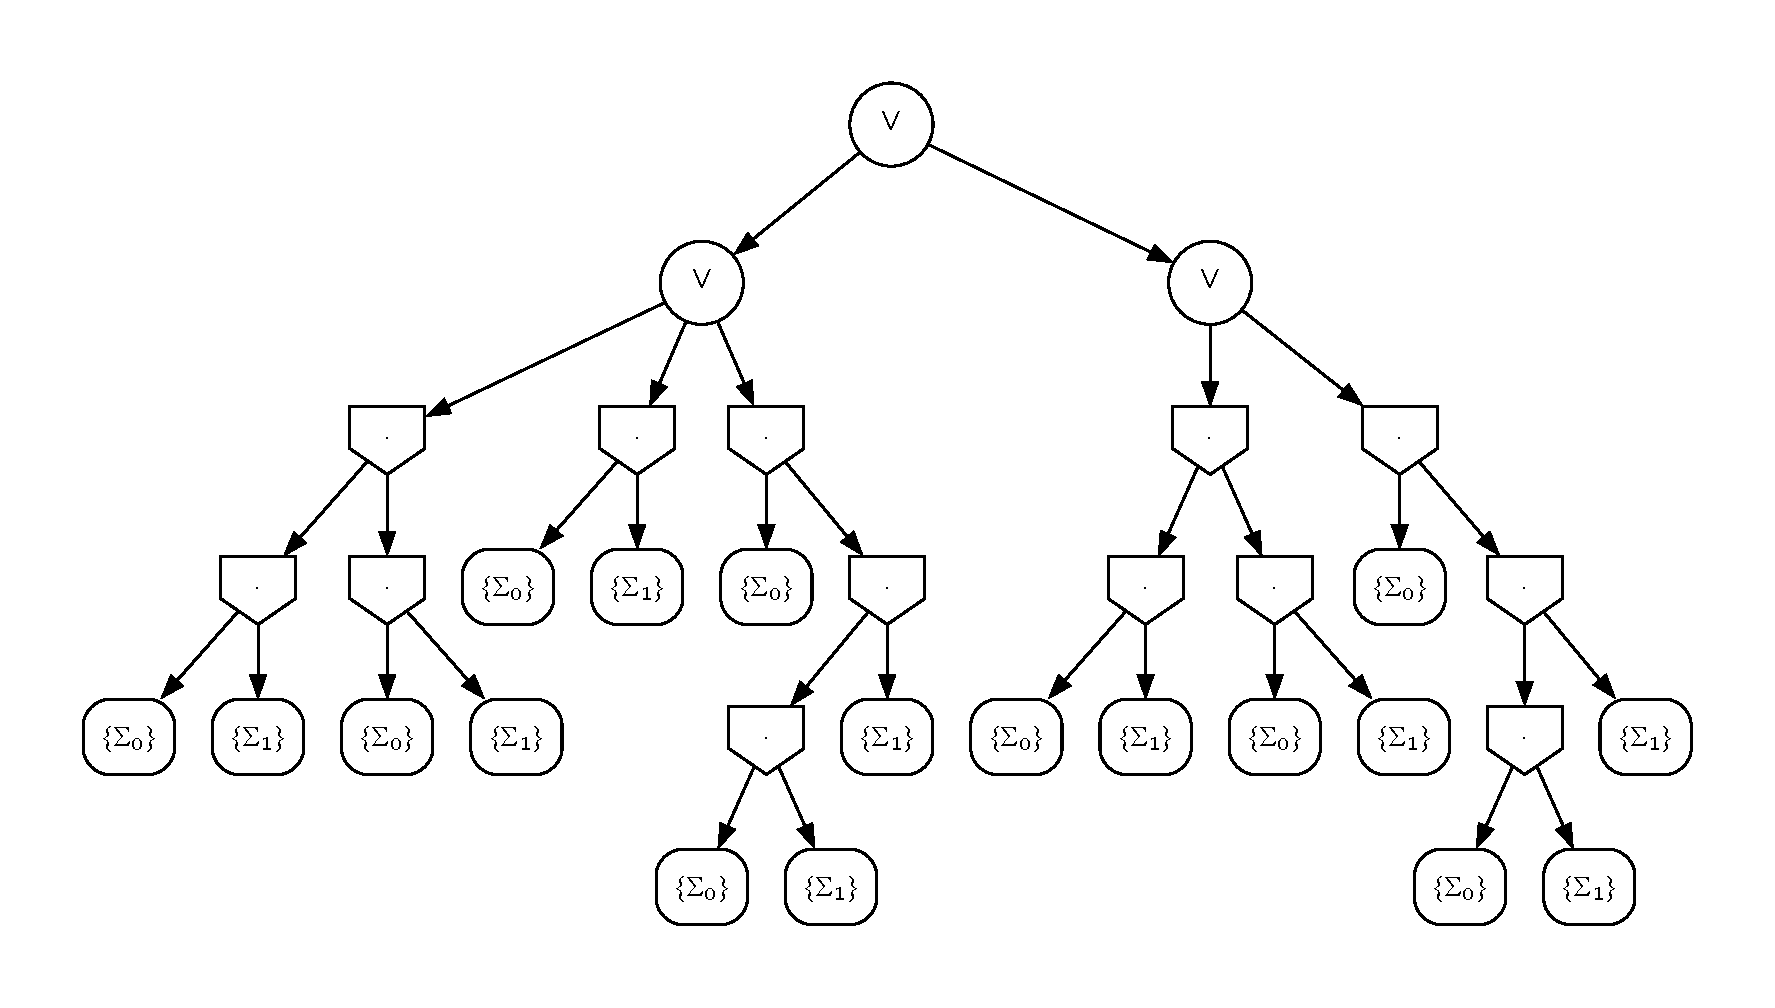
\includegraphics{figures/gre}
}
\end{center}
\vspace{-0.3cm}
\caption{Regular expression denoting $\mathcal{L}(G_\cap)$.}\label{fig:re_tree}
\end{wrapfigure}

As a concrete example, suppose we have the string, $\sigma=\texttt{( ) )}$ and wish to balance the parentheses. We will initially have the Levenshtein automaton, $A$, depicted in Fig.~\ref{fig:ex_atm}. To check for non-emptiness, we will perform the following procedure. Suppose we have a CNF CFG, $G'= \{S \rightarrow L R, S \rightarrow L F, S \rightarrow S S, F \rightarrow S R, L \rightarrow (, R \rightarrow )\}$ and let us assume an ordering of $S, F, L, R$ on $V$.

First, we need to order the automata states by increasing longest-path distance from $q_0$. One approach would be to topologically sort the adjacency matrix. While some form of sorting is unavoidable for arbitrary ANFAs, if we know ahead of time that our structure is a Levenshtein automaton, we can simply enumerate its state space by increasing Manhattan distance from the origin. % using, e.g., the Cantor pairing function to construct a valid ordering. This ordering will form the row and column indices of our intersection matrix, and each entry will represent the existence of some path between a two states yielding a given nonterminal.
So, a valid ordering on $Q$ would be $q_{00}, q_{01}, q_{10}, q_{11}, q_{20}, q_{21}, q_{30}, q_{31}$. Now, we want to compute $[\mathcal{L}(G')\cap \mathcal{L}(A) \neq \varnothing]$.

Under such an ordering, the adjacency matrix takes an upper triangular form and becomes the template for the initial parse chart, $M_0$ (Fig.~\ref{fig:initial_pc}). Each entry of this chart corresponds to a vector of expressions $E^{|V|}$ with at least one expression denoting a nonempty language. Likewise, the reachability matrix signifies a subset of state pairs which can participate in the language intersection. The adjacency and reachability matrices will always cover the expression vectors of the initial and final parse charts, respectively. In other words, we may safely ignore absent $\langle q, q'\rangle$ pairs in the reachability matrix, as these state pairs definitely cannot participate in the intersection.

From the reachability matrix we can construct the parse chart via matrix exponentiation. We note that n-step reachability constraints n-step parseability, i.e., $\sum_{i=0}^n A^i[q, q'] = \ws \vdash M_n[q, q', v] = \ws$, thus we can avoid substantial work via memoization. In this example, since $M_\infty[q_{00}, q_{31}, S] = \bs$, this implies that $\mathcal{L}(A)\cap \mathcal{L}(G') \neq \varnothing$, hence $\text{LED}(\sigma, G) = 1$. Using the same matrix, we will then perform a second pass to construct regular expressions representing finite languages for each nonempty constituent. Once again, we can skip $\langle q, q', v\rangle$ entries when $M_\infty[q, q', v] = \ws$ to hasten convergence.

Just as before, we will define $\boxplus, \boxtimes$ over GRE vectors, where $X \boxtimes Z = [X_x\cdot Z_z \mid (w\rightarrow xz) \in P]_{w\in V}$ and $X \boxplus Z= [ X_x\vee Z_z ]_{w\in V}$. Finally, we will repeat the matrix exponential, using $M_\infty$ in the binary domain as a guide. This allows us to construct the regular expression tree for $G_\cap = q_{00}Sq_{20}\vee q_{00}Sq_{31}$ shown in Fig.~\ref{fig:re_tree}. Once this regex is constructed, decoding becomes simply a matter of invoking \texttt{choose}$(G_\cap)$ to produce a concrete repair.

\clearpage

\section{Measuring the language intersection}

We will now attempt to put a probability distribution over the language intersection. We will start with a few cursory but illumative approaches, then proceed towards a more refined solution.

\subsection{Exact enumeration}

A brute force solution would be to generate every path and rank every one by its probability. It should be obvious why is unviable due its worst case complexity, but bears mentioning due to its global optimality. In certain cases, it can be realized when the intersection language is small.

To enumerate, we first need $|\mathcal{L}(e)|$, which is denoted $|e|$ for brevity.

\begin{definition}[Cardinality]
  $|e|: E \rightarrow \mathbb{N} =$ \begin{cases}
    1           & \text{if } R \in \Sigma \\
    x \times z  & \text{if } e = x \cdot z \\
    x + z       & \text{if } e = x \vee z
  \end{cases}\\
\end{definition}

\begin{theorem}[Enumeration]
  To enumerate, invoke $\bigcup_{i = 0}^{|R|}\{\texttt{enum}(R, i)\}$:\\

  $\texttt{enum}(e, n): E \times \mathbb{N} \rightarrow \Sigma^*$ = \begin{cases}
       e &\text{if } R \in \Sigma \\
       \texttt{enum}\big(x, \lfloor \frac{n}{|z|} \rfloor\big) \cdot \texttt{enum}\big(z,\, n \bmod |z|\big)  &\text{if } e = x \cdot z \\
       \texttt{enum}\big((x, z)_{\min(1, \lfloor\frac{n}{|x|}\rfloor)}, n-|x|\min(1, \lfloor\frac{n}{|x|}\rfloor)\big) &\text{if } e = x \vee z
  \end{cases}\\\\
\end{theorem}

\subsection{Mode collapse}

Ordinarily, we would use top-down PCFG sampling, however in the case of non-recursive CFGs as the case for $G_\cap$, this method is highly degenerate, exhibiting poor sample diversity. Consider an illustrative pathological case for top-down ancestral (TDA) sampling:

$$
S \rightarrow A\:B \: (0.9999) \hspace{20pt} S \rightarrow C\:C \: (0.0001)
$$

$$
A \rightarrow a \: (1) \hspace{20pt} B  \rightarrow b \: (1) \hspace{20pt} C  \rightarrow a \: \left(\frac{1}{26}\right) \mid \ldots \mid z \: \left(\frac{1}{26}\right)
$$\\

TDA sampling will almost always generate the string $a b$, but most of the language is concealed in the hidden branch, $S \rightarrow C C$. Although contrived example, it illustrates precisely why TDA sampling is unviable: we want a sampler that matches the true distribution over the finite CFL, not the PCFG's local approximation thereof.

\subsection{Ambiguity}

Another approach would be to sample trees and rerank them by their PCFG score. More pernicious is the issue of ambiguity. Since the CFG can be ambiguous, this causes certain repairs to be overrepresented, resulting in a subtle bias. Consider for example,

\begin{lemma}\label{lemma:ambiguity}
If the FSA, $\alpha$, is ambiguous, then the intersection grammar, $G_\cap$, can be ambiguous.
\end{lemma}

\begin{proof}
Let $\ell$ be the language defined by $G=\{S\rightarrow LR, L \rightarrow\texttt{(}, R \rightarrow\texttt{)}\}$, where $\alpha=L(\err\sigma, 2)$, the broken string $\err\sigma$ is $\texttt{)(}$, and $\mathcal{L}(G_\cap) = \ell \cap \mathcal{L}(\alpha)$. Then, $\mathcal{L}(G_\cap)$ contains the following two identical repairs: \texttt{\hlred{)}(\hlgreen{)}} with the parse $S \rightarrow q_{00}Lq_{21}\phantom{.}q_{21}Rq_{22}$, and \texttt{\hlorange{(}\hlorange{)}} with the parse $S \rightarrow q_{00}Lq_{11}\phantom{.}q_{11}Rq_{22}$.
\end{proof}

We would like the underlying sample space to be a proper set, \textit{not} a multiset.

\section{Implementation}

The implementation essentially consists of five stages, each dependent on its predecessor.

\begin{enumerate}
  \item $\texttt{lev\_build}: \Sigma^{|Q|-1} \times \mathbb{N}^{3} \rightarrow \text{NFA}$ -- constructs a Levenshtein NFA from the broken string.
  \item $\texttt{cfl\_fixpt}: \text{NFA} \times \text{CFG} \rightarrow \mathbb{B}^{|Q|\times |Q| \times |V|}$ -- computes the matrix exponential.
  \item $\texttt{reg\_build}: \mathbb{B}^{|Q|\times |Q| \times |V|} \times \text{CFG} \rightarrow \text{REG}$ -- constructs the regular expression for $G_\cap$.
  \item $\texttt{reg\_dcode}: \text{REG} \times \mathbb{N}^{|\Sigma|^{c\approx 3}} \hspace{-0.12cm}\rightarrow (\Sigma^* \times \mathbb{N})^{p\gg1}$ -- generates and scores a large number of repairs.
  \item $\texttt{sel\_top\_k}: (\Sigma^* \times \mathbb{N})^{p\gg1} \times \mathbb{N} \rightarrow (\Sigma^*)^{k\ll p}$ -- returns a small set of the most probable repairs.
\end{enumerate}

\noindent We will now explore the imperative pseudocode for each stage, starting with the Levenshtein automata constructor, which is a straightforward translation of the inference rules in Sec.~\ref{sec:repair_ex}.

\begin{algorithm}[H]
\caption{\texttt{lev\_build} pseudocode}
\label{alg:lev_build}
\begin{algorithmic}[1]
  \Procedure{\texttt{lev\_build}$(\sigma: \Sigma^n, d_{\max}: \mathbb{N})$}{} \Comment{Takes a string and maximum edit distance.}
  \State $Q, \delta \gets \varnothing$
  \For{$\langle h, j, i, k \rangle \textbf{ in } [0, n]^2\times[0, d_{\max}]^2$\vspace{1.34cm}}
    \State \vspace{-1.65cm}\[\hspace{0.5cm}\delta' \gets \!\left\{
        \begin{alignedat}{9}
          &\;& q_{h,i} &\hspace{-0.1cm}\overset{[\neq\sigma_{j+1}]}{\rightarrow} &q_{j,k} &\qquad& \text{if}\;& h = j   &\:\land\:& i = k-1  &\qquad& \duparrow\\[-2pt]
          && q_{h,i}   &\overset{[\neq\sigma_j]}{\rightarrow} &q_{j,k} &&       \text{if}\;& h = j-1 &\:\land\:& i = k-1  &&       \ddiagarrow\\[-2pt]
          && q_{h,i}   &\overset{[=\sigma_j]}{\rightarrow}    &q_{j,k} &&       \text{if}\;& h = j-1 &\:\land\:& i = k    &&       \drightarrow\\[-2pt]
          && q_{h,i}   &\overset{[=\sigma_j]}{\rightarrow}    &q_{j,k} &&       \text{if}\;& 1 \leq j - h - 1 \leq d_{\max} &\:\land\:& 1 \leq k - i \leq d_{\max}   && \knightarrow\;
        \end{alignedat}
      \right\phantom{\}}\]
    \State $Q \gets Q \cup \{\pi_1(\delta'), \pi_3(\delta')\}, \delta \gets \delta \cup \{\delta'\}$
  \EndFor
  \State $I \gets \{q_{0,0}\}, F \gets \{q_{i, j} \mid n - i + j \leq d_{\max}\}$
  \State \Return $\langle Q, \Sigma, \delta, I, F\rangle$  \Comment{Returns a Levenshtein automaton.}
\end{algorithmic}
\end{algorithm}

Next, the chart parser expects an acyclic NFA, a CNF grammar and returns a Boolean 3-tensor.

\begin{algorithm}[H]
\caption{\texttt{cfl\_fixpt} pseudocode}
\label{alg:cfl_fixpt}
\begin{algorithmic}[1]
\Require CFG must be in CNF and the NFA must be $\varepsilon$-free and acyclic (i.e, denote a finite langauge).
\Procedure{\texttt{cfl\_fixpt}$\big(\langle \Sigma, V, P, S\rangle: \text{CFG}, \langle Q, \Sigma, \delta, I, F\rangle: \text{NFA}\big)$}{}
\State $R: \mathbb{B}^{|Q|\times |Q|} \gets \big[\bs \textbf{ if } \exists \sigma \in \Sigma^+ \mid q \overset{\sigma}{\rightsquigarrow} q' \textbf{ else } \ws\big]_{q,\,q'\,:\, Q}$ \Comment{Solve for reachability matrix.}
\State $M: \mathbb{B}^{|Q|\times |Q| \times |V|} \gets \big[\bs \textbf{ if } \exists v: V, w: \Sigma \mid (v \rightarrow w) \in P \land (q \overset{s}{\rightarrow} q') \in \delta \textbf{ else } \ws\big]_{q,\,q'\,:\,Q,\,v\,:\,V}$
\For{$i \textbf{ in } \big[0, \lceil\log_2(|Q|)\rceil\big]$} \Comment{Solves matrix exponential, $\exp(M_0)$.}
\State $\textsc{done} \gets \bs$
\For{$\langle p, r, w \rangle \textbf{ in } Q^2\times V$} \Comment{Iterates one step of $M_{i+1} = M_i + M_i^2$.}
  \State $\textbf{if } M[p, r, w] \textbf{ or not } R[p, r] \textbf{ then continue}$
  \State $Q_{pr} \gets \{q: Q \mid R[p, q] \land R[q, r]\}$ \Comment{Consider reachable states between p and r.}
  \State $M[p, r, w] \gets \bs \textbf{ if } \exists q: Q_{pr}, x, z: V \mid M[p, q, x] \land M[q, r, z] \land (w \rightarrow x z) \in P \textbf { else } \ws$
  \State $\textbf{if } M[p, r, w] \textbf{ then } \textsc{done} \gets \ws$
\EndFor
\State $\textbf{if }\textsc{done} \textbf{ then break}$
\EndFor
\State \Return $M$ \Comment{Returns the completed parse chart.}
  \end{algorithmic}
\end{algorithm}

Note we may short-circuit in two places, if: $M_{i+1} = M_i$, or when two states $q, q'$ are unreachable. Once we obtain $M_\infty$, we can immediately tell whether $\ell_\cap \neq \varnothing$ by checking $M_\infty[q_{0,0}, q', S] = \bs$ for some $q': F$. Otherwise if no such $q'$ exists, then $\ell_\cap$ must be empty and $d_\max$ should be enlarged.

Now we can proceed to build the regular expression representing $\ell_\cap = \mathcal{L}(G_\cap)$.

\begin{algorithm}[H]
\caption{\texttt{reg\_build} pseudocode}
\label{alg:reg_build}
\begin{algorithmic}[1]
  \Procedure{\texttt{reg\_build}$\big(M_{\mathbb{B}}: \mathbb{B}^{|Q|\times |Q| \times |V|}, \langle \Sigma, V, P, S\rangle: \text{CFG}, \langle Q, \Sigma, \delta, I, F\rangle: \text{NFA}\big)$}{}
  \State $P: \mathbb{B}^{|Q|\times |Q|} \gets \big[\bs \textbf{ if } \exists q: Q, v, v': V \mid M_{\mathbb{B}}[p, q, v] \land M_{\mathbb{B}}[q, r, v'] \textbf{ else } \ws\big]_{p,\,r\,:\,Q}$
  \State $M: \text{REG}^{|Q|\times |Q| \times |V|} \gets \big[\{w \mid M[q, q', v] \land (q \overset{w}{\rightarrow} q') \in \delta \land (v\rightarrow w) \in P\}\big]_{q,\,q'\,:\, Q,\,v\,:\,V}$
  \For{$i \textbf{ in } \big[0, \lceil\log_2(|Q|)\rceil\big]$}
  \State $M' \gets M$
  \For{$\langle p, r, w \rangle \textbf{ in } Q^2\times V$}
  \State $\textbf{if not } M_\mathbb{B}[p, r, w] \textbf{ then continue}$
  \State $Q_{pr} \gets \{q: Q \mid P[p, q] \land P[q, r]\}$ \Comment{Consider parseable states between p and r.}\vspace{0.2cm}
  \State \vspace{-0.42cm}\[\hspace{0.62cm}M'[p, r, w] \gets M[p, r, w] \vee \bigvee_{\mathclap{\substack{q\,:\,Q_{pr}\\x,\,z\,:\,V}}} \big\{M[p, q, x]\cdot M[q, r, z] \mid (w \rightarrow x z) \in P\big\}\]\vspace{-0.2cm}
  \EndFor
  \State $\textbf{if } M=M' \textbf{ then break else } M \gets M'$
  \EndFor \vspace{0.2cm}
  \State \vspace{-0.42cm}\[\hspace{-8.5cm}\textbf{return }\bigvee_{\mathclap{q\,:\,I,\,q'\,:\,F}} M[q, q', S]\vspace{-0.8cm}\] \Comment{Union regexes for all total parses yielding S.}\vspace{0.31cm}
\end{algorithmic}
\end{algorithm}

Once we have the expression for $G_\cap$, we can decode it to rapidly produce a large set of candidates.

\begin{algorithm}[H]
  \caption{\texttt{reg\_dcode} pseudocode}
  \label{alg:reg_dcode}
  \begin{algorithmic}[1]
  \Require We expect the shortest word to exceed the Markov order in length, $c < |\sigma|, \forall\sigma: \mathcal{L}(e)$.
  \Procedure{\texttt{reg\_dcode}$\big(e: \text{REG}, C: \mathbb{N}^{|\Sigma|^{c\approx 3}}\big)$}{}
    \State $\mathcal{T} \gets [], \mathcal{E} \gets \big[\langle \varepsilon^{c-1}, e\cdot \varepsilon^{c-1}, 0\rangle\big]$ \Comment{Initialize total and partial trajectories.}\vspace{0.5cm}
    \State \vspace{-0.55cm}\[\hspace{-4.71cm}\textbf{let } P(s: \Sigma \mid \sigma: \Sigma^*) =_{\text{def}} \frac{C[\sigma_{|\sigma| - c + 1, |\sigma|}\cdot s]+ 1}{\sum_{s' \in \Sigma} C[\sigma_{|\sigma| - c + 1, |\sigma|}\cdot s']}\vspace{-0.7cm}\]\Comment{Define Markov transition probability.}\vspace{0.3cm}
    \Repeat
        \State $\langle\sigma, e, p\rangle \gets \textbf{pop } \mathcal{E}_0 \textbf{ off }\mathcal{E}$
        \State $\mathcal{E}' \gets \big[\langle\sigma\cdot a, \partial_a e, p + \ln P(a\mid \sigma) \rangle \mid a \in \texttt{follow}(e)\big]$
        \State $\mathcal{T}\hspace{0.05cm} \gets \mathcal{T} \texttt{++} \big[\langle \sigma, p \rangle \mid \langle \sigma, e, p\rangle \in \mathcal{E}' \land \varepsilon \in \mathcal{L}(e)\big]$
        \State $\mathcal{E}\phantom{'} \gets \big[\langle\sigma, e, p\rangle \in (\mathcal{E} \texttt{++} \mathcal{E}')\textbf{ sorted by } p\big]$
    \Until{interrupted or $\mathcal{E}$ is empty.}
    \State \Return $\mathcal{T}$
  \end{algorithmic}
\end{algorithm}

Now we are ready to skim off the highest probability repairs using a standard selection algorithm.

\begin{algorithm}[H]
  \caption{\texttt{sel\_top\_k} pseudocode}
  \label{alg:sel_top_k}
  \begin{algorithmic}[1]
    \Procedure{\texttt{sel\_top\_k}$\big(l: (\Sigma^* \times \mathbb{N})^{p\gg1}, k: \mathbb{N}\big)$}{}
    \State $\hat{A}: (\Sigma^* \times \mathbb{N})^* \gets [l_0]}$ \Comment{Initialize a priority queue of nearly-optimal repairs.}
    \For{$\langle\sigma, s\rangle \textbf{ in } l$}
      \State $\textbf{if } s < \pi_2(\hat{A}_{|\hat{A}|}) \textbf{ then insert } \langle\sigma, s\rangle \textbf{ into } \hat{A} \textbf{ and drop } \hat{A}_{|k + 1|} \textbf{ if } |\hat{A}| > k$
    \EndFor
    \State \Return $[\pi_1(a) \mid a \in \hat{A}]$ \Comment{Return top-k candidates.}
  \end{algorithmic}
\end{algorithm}

  Finally, we have our shortlist of repairs and after postprocessing, can present them to the user.

\clearpage\subsection{GPU translation}

Each stage is easily translatable to a GPU format, especially matrix multiplication which GPUs are specifically designed to accelerate.

We will make the simplifying assumption that each GPU kernel is a pure function that takes as input a coordinate triple $r, c, v: \mathbb{N}$ and one or more flat buffers $b_1: \mathbb{N}^{d_1}, \ldots b_n: \mathbb{N}^{d_n}$, does some arithmetic, and returns a single buffer $b_{\text{out}}: \mathbb{N}^{d}$.

Morally, each $\langle r, c, v\rangle$ triple will dispatch a single independent thread which reads from the input buffers and has exclusive write access to a contiguous region of the output buffer. Absent a GPU, this can be rewritten as a triply-nested loop subject to latency overhead. On a GPU, threads will effectively run simultaneously but memory must be sized ahead of time as no dynamic allocation is allowed during a GPU kernel's execution.

For CFG and NFA datatypes, we elect to use a dense representation $\mathbb{B}^{|V|\times|V|\times|V|}$ and $\mathbb{B}^{|Q|\times|Q|\times |\Sigma|}$ due to the tripartite coordinate structure and thread dispatching API. While these datatypes can be encoded sparsely as $\mathbb{N}^{3|P|}$ and $\mathbb{N}^{3|\delta|}$, for most repair instances and memory configurations representation size is not a bottleneck. It will be helpful to define two indices $\texttt{enc}: \Sigma \rightarrow 2^V$ and $\texttt{dec}: V \rightarrow 2^\Sigma$ for nonterminal encoding and decoding, and bijections $\Sigma \leftrightarrow \mathbb{N}$, $V \leftrightarrow \mathbb{N}$ for getting into and out of the integer domain -- these we omit for brevity but are trivial to define.

The REG datatype is slightly more complex to flatten, as being an algebraic datatype it can be simplified in various ways.\ldots

\clearpage\bibliography{../bib/acmart}

\pagebreak\appendix

\section{Levenshtein Automata Matrices}

These are useful for visually checking different implementations.

\begin{figure}[H]
  \begin{center}
    \resizebox{0.45\textwidth}{!}{%
      \begin{tikzpicture}[x=0.3cm, y=0.3cm, draw=gray, very thin]
  \path[fill=white] (0,13) rectangle ++(1,1);
  \path[fill=black] (1,13) rectangle ++(1,1);
  \path[fill=black] (2,13) rectangle ++(1,1);
  \path[fill=black] (3,13) rectangle ++(1,1);
  \path[fill=white] (4,13) rectangle ++(1,1);
  \path[fill=black] (5,13) rectangle ++(1,1);
  \path[fill=white] (6,13) rectangle ++(1,1);
  \path[fill=white] (7,13) rectangle ++(1,1);
  \path[fill=white] (8,13) rectangle ++(1,1);
  \path[fill=white] (9,13) rectangle ++(1,1);
  \path[fill=white] (10,13) rectangle ++(1,1);
  \path[fill=white] (11,13) rectangle ++(1,1);
  \path[fill=white] (12,13) rectangle ++(1,1);
  \path[fill=white] (13,13) rectangle ++(1,1);
  \path[fill=white] (0,12) rectangle ++(1,1);
  \path[fill=white] (1,12) rectangle ++(1,1);
  \path[fill=white] (2,12) rectangle ++(1,1);
  \path[fill=black] (3,12) rectangle ++(1,1);
  \path[fill=white] (4,12) rectangle ++(1,1);
  \path[fill=white] (5,12) rectangle ++(1,1);
  \path[fill=white] (6,12) rectangle ++(1,1);
  \path[fill=white] (7,12) rectangle ++(1,1);
  \path[fill=white] (8,12) rectangle ++(1,1);
  \path[fill=white] (9,12) rectangle ++(1,1);
  \path[fill=white] (10,12) rectangle ++(1,1);
  \path[fill=white] (11,12) rectangle ++(1,1);
  \path[fill=white] (12,12) rectangle ++(1,1);
  \path[fill=white] (13,12) rectangle ++(1,1);
  \path[fill=white] (0,11) rectangle ++(1,1);
  \path[fill=white] (1,11) rectangle ++(1,1);
  \path[fill=white] (2,11) rectangle ++(1,1);
  \path[fill=black] (3,11) rectangle ++(1,1);
  \path[fill=black] (4,11) rectangle ++(1,1);
  \path[fill=black] (5,11) rectangle ++(1,1);
  \path[fill=white] (6,11) rectangle ++(1,1);
  \path[fill=black] (7,11) rectangle ++(1,1);
  \path[fill=white] (8,11) rectangle ++(1,1);
  \path[fill=white] (9,11) rectangle ++(1,1);
  \path[fill=white] (10,11) rectangle ++(1,1);
  \path[fill=white] (11,11) rectangle ++(1,1);
  \path[fill=white] (12,11) rectangle ++(1,1);
  \path[fill=white] (13,11) rectangle ++(1,1);
  \path[fill=white] (0,10) rectangle ++(1,1);
  \path[fill=white] (1,10) rectangle ++(1,1);
  \path[fill=white] (2,10) rectangle ++(1,1);
  \path[fill=white] (3,10) rectangle ++(1,1);
  \path[fill=white] (4,10) rectangle ++(1,1);
  \path[fill=black] (5,10) rectangle ++(1,1);
  \path[fill=white] (6,10) rectangle ++(1,1);
  \path[fill=white] (7,10) rectangle ++(1,1);
  \path[fill=white] (8,10) rectangle ++(1,1);
  \path[fill=white] (9,10) rectangle ++(1,1);
  \path[fill=white] (10,10) rectangle ++(1,1);
  \path[fill=white] (11,10) rectangle ++(1,1);
  \path[fill=white] (12,10) rectangle ++(1,1);
  \path[fill=white] (13,10) rectangle ++(1,1);
  \path[fill=white] (0,9) rectangle ++(1,1);
  \path[fill=white] (1,9) rectangle ++(1,1);
  \path[fill=white] (2,9) rectangle ++(1,1);
  \path[fill=white] (3,9) rectangle ++(1,1);
  \path[fill=white] (4,9) rectangle ++(1,1);
  \path[fill=black] (5,9) rectangle ++(1,1);
  \path[fill=black] (6,9) rectangle ++(1,1);
  \path[fill=black] (7,9) rectangle ++(1,1);
  \path[fill=white] (8,9) rectangle ++(1,1);
  \path[fill=black] (9,9) rectangle ++(1,1);
  \path[fill=white] (10,9) rectangle ++(1,1);
  \path[fill=white] (11,9) rectangle ++(1,1);
  \path[fill=white] (12,9) rectangle ++(1,1);
  \path[fill=white] (13,9) rectangle ++(1,1);
  \path[fill=white] (0,8) rectangle ++(1,1);
  \path[fill=white] (1,8) rectangle ++(1,1);
  \path[fill=white] (2,8) rectangle ++(1,1);
  \path[fill=white] (3,8) rectangle ++(1,1);
  \path[fill=white] (4,8) rectangle ++(1,1);
  \path[fill=white] (5,8) rectangle ++(1,1);
  \path[fill=white] (6,8) rectangle ++(1,1);
  \path[fill=black] (7,8) rectangle ++(1,1);
  \path[fill=white] (8,8) rectangle ++(1,1);
  \path[fill=white] (9,8) rectangle ++(1,1);
  \path[fill=white] (10,8) rectangle ++(1,1);
  \path[fill=white] (11,8) rectangle ++(1,1);
  \path[fill=white] (12,8) rectangle ++(1,1);
  \path[fill=white] (13,8) rectangle ++(1,1);
  \path[fill=white] (0,7) rectangle ++(1,1);
  \path[fill=white] (1,7) rectangle ++(1,1);
  \path[fill=white] (2,7) rectangle ++(1,1);
  \path[fill=white] (3,7) rectangle ++(1,1);
  \path[fill=white] (4,7) rectangle ++(1,1);
  \path[fill=white] (5,7) rectangle ++(1,1);
  \path[fill=white] (6,7) rectangle ++(1,1);
  \path[fill=black] (7,7) rectangle ++(1,1);
  \path[fill=black] (8,7) rectangle ++(1,1);
  \path[fill=black] (9,7) rectangle ++(1,1);
  \path[fill=white] (10,7) rectangle ++(1,1);
  \path[fill=black] (11,7) rectangle ++(1,1);
  \path[fill=white] (12,7) rectangle ++(1,1);
  \path[fill=white] (13,7) rectangle ++(1,1);
  \path[fill=white] (0,6) rectangle ++(1,1);
  \path[fill=white] (1,6) rectangle ++(1,1);
  \path[fill=white] (2,6) rectangle ++(1,1);
  \path[fill=white] (3,6) rectangle ++(1,1);
  \path[fill=white] (4,6) rectangle ++(1,1);
  \path[fill=white] (5,6) rectangle ++(1,1);
  \path[fill=white] (6,6) rectangle ++(1,1);
  \path[fill=white] (7,6) rectangle ++(1,1);
  \path[fill=white] (8,6) rectangle ++(1,1);
  \path[fill=black] (9,6) rectangle ++(1,1);
  \path[fill=white] (10,6) rectangle ++(1,1);
  \path[fill=white] (11,6) rectangle ++(1,1);
  \path[fill=white] (12,6) rectangle ++(1,1);
  \path[fill=white] (13,6) rectangle ++(1,1);
  \path[fill=white] (0,5) rectangle ++(1,1);
  \path[fill=white] (1,5) rectangle ++(1,1);
  \path[fill=white] (2,5) rectangle ++(1,1);
  \path[fill=white] (3,5) rectangle ++(1,1);
  \path[fill=white] (4,5) rectangle ++(1,1);
  \path[fill=white] (5,5) rectangle ++(1,1);
  \path[fill=white] (6,5) rectangle ++(1,1);
  \path[fill=white] (7,5) rectangle ++(1,1);
  \path[fill=white] (8,5) rectangle ++(1,1);
  \path[fill=black] (9,5) rectangle ++(1,1);
  \path[fill=black] (10,5) rectangle ++(1,1);
  \path[fill=black] (11,5) rectangle ++(1,1);
  \path[fill=white] (12,5) rectangle ++(1,1);
  \path[fill=black] (13,5) rectangle ++(1,1);
  \path[fill=white] (0,4) rectangle ++(1,1);
  \path[fill=white] (1,4) rectangle ++(1,1);
  \path[fill=white] (2,4) rectangle ++(1,1);
  \path[fill=white] (3,4) rectangle ++(1,1);
  \path[fill=white] (4,4) rectangle ++(1,1);
  \path[fill=white] (5,4) rectangle ++(1,1);
  \path[fill=white] (6,4) rectangle ++(1,1);
  \path[fill=white] (7,4) rectangle ++(1,1);
  \path[fill=white] (8,4) rectangle ++(1,1);
  \path[fill=white] (9,4) rectangle ++(1,1);
  \path[fill=white] (10,4) rectangle ++(1,1);
  \path[fill=black] (11,4) rectangle ++(1,1);
  \path[fill=white] (12,4) rectangle ++(1,1);
  \path[fill=white] (13,4) rectangle ++(1,1);
  \path[fill=white] (0,3) rectangle ++(1,1);
  \path[fill=white] (1,3) rectangle ++(1,1);
  \path[fill=white] (2,3) rectangle ++(1,1);
  \path[fill=white] (3,3) rectangle ++(1,1);
  \path[fill=white] (4,3) rectangle ++(1,1);
  \path[fill=white] (5,3) rectangle ++(1,1);
  \path[fill=white] (6,3) rectangle ++(1,1);
  \path[fill=white] (7,3) rectangle ++(1,1);
  \path[fill=white] (8,3) rectangle ++(1,1);
  \path[fill=white] (9,3) rectangle ++(1,1);
  \path[fill=white] (10,3) rectangle ++(1,1);
  \path[fill=black] (11,3) rectangle ++(1,1);
  \path[fill=black] (12,3) rectangle ++(1,1);
  \path[fill=black] (13,3) rectangle ++(1,1);
  \path[fill=white] (0,2) rectangle ++(1,1);
  \path[fill=white] (1,2) rectangle ++(1,1);
  \path[fill=white] (2,2) rectangle ++(1,1);
  \path[fill=white] (3,2) rectangle ++(1,1);
  \path[fill=white] (4,2) rectangle ++(1,1);
  \path[fill=white] (5,2) rectangle ++(1,1);
  \path[fill=white] (6,2) rectangle ++(1,1);
  \path[fill=white] (7,2) rectangle ++(1,1);
  \path[fill=white] (8,2) rectangle ++(1,1);
  \path[fill=white] (9,2) rectangle ++(1,1);
  \path[fill=white] (10,2) rectangle ++(1,1);
  \path[fill=white] (11,2) rectangle ++(1,1);
  \path[fill=white] (12,2) rectangle ++(1,1);
  \path[fill=black] (13,2) rectangle ++(1,1);
  \path[fill=white] (0,1) rectangle ++(1,1);
  \path[fill=white] (1,1) rectangle ++(1,1);
  \path[fill=white] (2,1) rectangle ++(1,1);
  \path[fill=white] (3,1) rectangle ++(1,1);
  \path[fill=white] (4,1) rectangle ++(1,1);
  \path[fill=white] (5,1) rectangle ++(1,1);
  \path[fill=white] (6,1) rectangle ++(1,1);
  \path[fill=white] (7,1) rectangle ++(1,1);
  \path[fill=white] (8,1) rectangle ++(1,1);
  \path[fill=white] (9,1) rectangle ++(1,1);
  \path[fill=white] (10,1) rectangle ++(1,1);
  \path[fill=white] (11,1) rectangle ++(1,1);
  \path[fill=white] (12,1) rectangle ++(1,1);
  \path[fill=black] (13,1) rectangle ++(1,1);
  \path[fill=white] (0,0) rectangle ++(1,1);
  \path[fill=white] (1,0) rectangle ++(1,1);
  \path[fill=white] (2,0) rectangle ++(1,1);
  \path[fill=white] (3,0) rectangle ++(1,1);
  \path[fill=white] (4,0) rectangle ++(1,1);
  \path[fill=white] (5,0) rectangle ++(1,1);
  \path[fill=white] (6,0) rectangle ++(1,1);
  \path[fill=white] (7,0) rectangle ++(1,1);
  \path[fill=white] (8,0) rectangle ++(1,1);
  \path[fill=white] (9,0) rectangle ++(1,1);
  \path[fill=white] (10,0) rectangle ++(1,1);
  \path[fill=white] (11,0) rectangle ++(1,1);
  \path[fill=white] (12,0) rectangle ++(1,1);
  \path[fill=white] (13,0) rectangle ++(1,1);
\end{tikzpicture}

\begin{tikzpicture}[x=0.3cm, y=0.3cm, draw=gray, very thin]
  \path[fill=white] (0,13) rectangle ++(1,1);
  \path[fill=black] (1,13) rectangle ++(1,1);
  \path[fill=black] (2,13) rectangle ++(1,1);
  \path[fill=black] (3,13) rectangle ++(1,1);
  \path[fill=black] (4,13) rectangle ++(1,1);
  \path[fill=black] (5,13) rectangle ++(1,1);
  \path[fill=black] (6,13) rectangle ++(1,1);
  \path[fill=black] (7,13) rectangle ++(1,1);
  \path[fill=black] (8,13) rectangle ++(1,1);
  \path[fill=black] (9,13) rectangle ++(1,1);
  \path[fill=black] (10,13) rectangle ++(1,1);
  \path[fill=black] (11,13) rectangle ++(1,1);
  \path[fill=black] (12,13) rectangle ++(1,1);
  \path[fill=black] (13,13) rectangle ++(1,1);
  \path[fill=white] (0,12) rectangle ++(1,1);
  \path[fill=white] (1,12) rectangle ++(1,1);
  \path[fill=white] (2,12) rectangle ++(1,1);
  \path[fill=black] (3,12) rectangle ++(1,1);
  \path[fill=white] (4,12) rectangle ++(1,1);
  \path[fill=black] (5,12) rectangle ++(1,1);
  \path[fill=white] (6,12) rectangle ++(1,1);
  \path[fill=black] (7,12) rectangle ++(1,1);
  \path[fill=white] (8,12) rectangle ++(1,1);
  \path[fill=black] (9,12) rectangle ++(1,1);
  \path[fill=white] (10,12) rectangle ++(1,1);
  \path[fill=black] (11,12) rectangle ++(1,1);
  \path[fill=white] (12,12) rectangle ++(1,1);
  \path[fill=black] (13,12) rectangle ++(1,1);
  \path[fill=white] (0,11) rectangle ++(1,1);
  \path[fill=white] (1,11) rectangle ++(1,1);
  \path[fill=white] (2,11) rectangle ++(1,1);
  \path[fill=black] (3,11) rectangle ++(1,1);
  \path[fill=black] (4,11) rectangle ++(1,1);
  \path[fill=black] (5,11) rectangle ++(1,1);
  \path[fill=black] (6,11) rectangle ++(1,1);
  \path[fill=black] (7,11) rectangle ++(1,1);
  \path[fill=black] (8,11) rectangle ++(1,1);
  \path[fill=black] (9,11) rectangle ++(1,1);
  \path[fill=black] (10,11) rectangle ++(1,1);
  \path[fill=black] (11,11) rectangle ++(1,1);
  \path[fill=black] (12,11) rectangle ++(1,1);
  \path[fill=black] (13,11) rectangle ++(1,1);
  \path[fill=white] (0,10) rectangle ++(1,1);
  \path[fill=white] (1,10) rectangle ++(1,1);
  \path[fill=white] (2,10) rectangle ++(1,1);
  \path[fill=white] (3,10) rectangle ++(1,1);
  \path[fill=white] (4,10) rectangle ++(1,1);
  \path[fill=black] (5,10) rectangle ++(1,1);
  \path[fill=white] (6,10) rectangle ++(1,1);
  \path[fill=black] (7,10) rectangle ++(1,1);
  \path[fill=white] (8,10) rectangle ++(1,1);
  \path[fill=black] (9,10) rectangle ++(1,1);
  \path[fill=white] (10,10) rectangle ++(1,1);
  \path[fill=black] (11,10) rectangle ++(1,1);
  \path[fill=white] (12,10) rectangle ++(1,1);
  \path[fill=black] (13,10) rectangle ++(1,1);
  \path[fill=white] (0,9) rectangle ++(1,1);
  \path[fill=white] (1,9) rectangle ++(1,1);
  \path[fill=white] (2,9) rectangle ++(1,1);
  \path[fill=white] (3,9) rectangle ++(1,1);
  \path[fill=white] (4,9) rectangle ++(1,1);
  \path[fill=black] (5,9) rectangle ++(1,1);
  \path[fill=black] (6,9) rectangle ++(1,1);
  \path[fill=black] (7,9) rectangle ++(1,1);
  \path[fill=black] (8,9) rectangle ++(1,1);
  \path[fill=black] (9,9) rectangle ++(1,1);
  \path[fill=black] (10,9) rectangle ++(1,1);
  \path[fill=black] (11,9) rectangle ++(1,1);
  \path[fill=black] (12,9) rectangle ++(1,1);
  \path[fill=black] (13,9) rectangle ++(1,1);
  \path[fill=white] (0,8) rectangle ++(1,1);
  \path[fill=white] (1,8) rectangle ++(1,1);
  \path[fill=white] (2,8) rectangle ++(1,1);
  \path[fill=white] (3,8) rectangle ++(1,1);
  \path[fill=white] (4,8) rectangle ++(1,1);
  \path[fill=white] (5,8) rectangle ++(1,1);
  \path[fill=white] (6,8) rectangle ++(1,1);
  \path[fill=black] (7,8) rectangle ++(1,1);
  \path[fill=white] (8,8) rectangle ++(1,1);
  \path[fill=black] (9,8) rectangle ++(1,1);
  \path[fill=white] (10,8) rectangle ++(1,1);
  \path[fill=black] (11,8) rectangle ++(1,1);
  \path[fill=white] (12,8) rectangle ++(1,1);
  \path[fill=black] (13,8) rectangle ++(1,1);
  \path[fill=white] (0,7) rectangle ++(1,1);
  \path[fill=white] (1,7) rectangle ++(1,1);
  \path[fill=white] (2,7) rectangle ++(1,1);
  \path[fill=white] (3,7) rectangle ++(1,1);
  \path[fill=white] (4,7) rectangle ++(1,1);
  \path[fill=white] (5,7) rectangle ++(1,1);
  \path[fill=white] (6,7) rectangle ++(1,1);
  \path[fill=black] (7,7) rectangle ++(1,1);
  \path[fill=black] (8,7) rectangle ++(1,1);
  \path[fill=black] (9,7) rectangle ++(1,1);
  \path[fill=black] (10,7) rectangle ++(1,1);
  \path[fill=black] (11,7) rectangle ++(1,1);
  \path[fill=black] (12,7) rectangle ++(1,1);
  \path[fill=black] (13,7) rectangle ++(1,1);
  \path[fill=white] (0,6) rectangle ++(1,1);
  \path[fill=white] (1,6) rectangle ++(1,1);
  \path[fill=white] (2,6) rectangle ++(1,1);
  \path[fill=white] (3,6) rectangle ++(1,1);
  \path[fill=white] (4,6) rectangle ++(1,1);
  \path[fill=white] (5,6) rectangle ++(1,1);
  \path[fill=white] (6,6) rectangle ++(1,1);
  \path[fill=white] (7,6) rectangle ++(1,1);
  \path[fill=white] (8,6) rectangle ++(1,1);
  \path[fill=black] (9,6) rectangle ++(1,1);
  \path[fill=white] (10,6) rectangle ++(1,1);
  \path[fill=black] (11,6) rectangle ++(1,1);
  \path[fill=white] (12,6) rectangle ++(1,1);
  \path[fill=black] (13,6) rectangle ++(1,1);
  \path[fill=white] (0,5) rectangle ++(1,1);
  \path[fill=white] (1,5) rectangle ++(1,1);
  \path[fill=white] (2,5) rectangle ++(1,1);
  \path[fill=white] (3,5) rectangle ++(1,1);
  \path[fill=white] (4,5) rectangle ++(1,1);
  \path[fill=white] (5,5) rectangle ++(1,1);
  \path[fill=white] (6,5) rectangle ++(1,1);
  \path[fill=white] (7,5) rectangle ++(1,1);
  \path[fill=white] (8,5) rectangle ++(1,1);
  \path[fill=black] (9,5) rectangle ++(1,1);
  \path[fill=black] (10,5) rectangle ++(1,1);
  \path[fill=black] (11,5) rectangle ++(1,1);
  \path[fill=black] (12,5) rectangle ++(1,1);
  \path[fill=black] (13,5) rectangle ++(1,1);
  \path[fill=white] (0,4) rectangle ++(1,1);
  \path[fill=white] (1,4) rectangle ++(1,1);
  \path[fill=white] (2,4) rectangle ++(1,1);
  \path[fill=white] (3,4) rectangle ++(1,1);
  \path[fill=white] (4,4) rectangle ++(1,1);
  \path[fill=white] (5,4) rectangle ++(1,1);
  \path[fill=white] (6,4) rectangle ++(1,1);
  \path[fill=white] (7,4) rectangle ++(1,1);
  \path[fill=white] (8,4) rectangle ++(1,1);
  \path[fill=white] (9,4) rectangle ++(1,1);
  \path[fill=white] (10,4) rectangle ++(1,1);
  \path[fill=black] (11,4) rectangle ++(1,1);
  \path[fill=white] (12,4) rectangle ++(1,1);
  \path[fill=black] (13,4) rectangle ++(1,1);
  \path[fill=white] (0,3) rectangle ++(1,1);
  \path[fill=white] (1,3) rectangle ++(1,1);
  \path[fill=white] (2,3) rectangle ++(1,1);
  \path[fill=white] (3,3) rectangle ++(1,1);
  \path[fill=white] (4,3) rectangle ++(1,1);
  \path[fill=white] (5,3) rectangle ++(1,1);
  \path[fill=white] (6,3) rectangle ++(1,1);
  \path[fill=white] (7,3) rectangle ++(1,1);
  \path[fill=white] (8,3) rectangle ++(1,1);
  \path[fill=white] (9,3) rectangle ++(1,1);
  \path[fill=white] (10,3) rectangle ++(1,1);
  \path[fill=black] (11,3) rectangle ++(1,1);
  \path[fill=black] (12,3) rectangle ++(1,1);
  \path[fill=black] (13,3) rectangle ++(1,1);
  \path[fill=white] (0,2) rectangle ++(1,1);
  \path[fill=white] (1,2) rectangle ++(1,1);
  \path[fill=white] (2,2) rectangle ++(1,1);
  \path[fill=white] (3,2) rectangle ++(1,1);
  \path[fill=white] (4,2) rectangle ++(1,1);
  \path[fill=white] (5,2) rectangle ++(1,1);
  \path[fill=white] (6,2) rectangle ++(1,1);
  \path[fill=white] (7,2) rectangle ++(1,1);
  \path[fill=white] (8,2) rectangle ++(1,1);
  \path[fill=white] (9,2) rectangle ++(1,1);
  \path[fill=white] (10,2) rectangle ++(1,1);
  \path[fill=white] (11,2) rectangle ++(1,1);
  \path[fill=white] (12,2) rectangle ++(1,1);
  \path[fill=black] (13,2) rectangle ++(1,1);
  \path[fill=white] (0,1) rectangle ++(1,1);
  \path[fill=white] (1,1) rectangle ++(1,1);
  \path[fill=white] (2,1) rectangle ++(1,1);
  \path[fill=white] (3,1) rectangle ++(1,1);
  \path[fill=white] (4,1) rectangle ++(1,1);
  \path[fill=white] (5,1) rectangle ++(1,1);
  \path[fill=white] (6,1) rectangle ++(1,1);
  \path[fill=white] (7,1) rectangle ++(1,1);
  \path[fill=white] (8,1) rectangle ++(1,1);
  \path[fill=white] (9,1) rectangle ++(1,1);
  \path[fill=white] (10,1) rectangle ++(1,1);
  \path[fill=white] (11,1) rectangle ++(1,1);
  \path[fill=white] (12,1) rectangle ++(1,1);
  \path[fill=black] (13,1) rectangle ++(1,1);
  \path[fill=white] (0,0) rectangle ++(1,1);
  \path[fill=white] (1,0) rectangle ++(1,1);
  \path[fill=white] (2,0) rectangle ++(1,1);
  \path[fill=white] (3,0) rectangle ++(1,1);
  \path[fill=white] (4,0) rectangle ++(1,1);
  \path[fill=white] (5,0) rectangle ++(1,1);
  \path[fill=white] (6,0) rectangle ++(1,1);
  \path[fill=white] (7,0) rectangle ++(1,1);
  \path[fill=white] (8,0) rectangle ++(1,1);
  \path[fill=white] (9,0) rectangle ++(1,1);
  \path[fill=white] (10,0) rectangle ++(1,1);
  \path[fill=white] (11,0) rectangle ++(1,1);
  \path[fill=white] (12,0) rectangle ++(1,1);
  \path[fill=white] (13,0) rectangle ++(1,1);
\end{tikzpicture}
    }
  \end{center}
  \caption{Lev(|\sigma|=6, \Delta=1) adjacency and reachability matrices.}
\end{figure}

\begin{figure}[H]
  \begin{center}
    \resizebox{0.45\textwidth}{!}{%
      \begin{tikzpicture}[x=0.3cm, y=0.3cm, draw=gray, very thin]
\path[fill=white] (0,20) rectangle ++(1,1);
\path[fill=black] (1,20) rectangle ++(1,1);
\path[fill=black] (2,20) rectangle ++(1,1);
\path[fill=white] (3,20) rectangle ++(1,1);
\path[fill=black] (4,20) rectangle ++(1,1);
\path[fill=white] (5,20) rectangle ++(1,1);
\path[fill=white] (6,20) rectangle ++(1,1);
\path[fill=black] (7,20) rectangle ++(1,1);
\path[fill=white] (8,20) rectangle ++(1,1);
\path[fill=white] (9,20) rectangle ++(1,1);
\path[fill=white] (10,20) rectangle ++(1,1);
\path[fill=white] (11,20) rectangle ++(1,1);
\path[fill=black] (12,20) rectangle ++(1,1);
\path[fill=white] (13,20) rectangle ++(1,1);
\path[fill=white] (14,20) rectangle ++(1,1);
\path[fill=white] (15,20) rectangle ++(1,1);
\path[fill=white] (16,20) rectangle ++(1,1);
\path[fill=white] (17,20) rectangle ++(1,1);
\path[fill=white] (18,20) rectangle ++(1,1);
\path[fill=white] (19,20) rectangle ++(1,1);
\path[fill=white] (20,20) rectangle ++(1,1);
\path[fill=white] (0,19) rectangle ++(1,1);
\path[fill=white] (1,19) rectangle ++(1,1);
\path[fill=white] (2,19) rectangle ++(1,1);
\path[fill=black] (3,19) rectangle ++(1,1);
\path[fill=black] (4,19) rectangle ++(1,1);
\path[fill=white] (5,19) rectangle ++(1,1);
\path[fill=black] (6,19) rectangle ++(1,1);
\path[fill=white] (7,19) rectangle ++(1,1);
\path[fill=white] (8,19) rectangle ++(1,1);
\path[fill=black] (9,19) rectangle ++(1,1);
\path[fill=white] (10,19) rectangle ++(1,1);
\path[fill=white] (11,19) rectangle ++(1,1);
\path[fill=white] (12,19) rectangle ++(1,1);
\path[fill=white] (13,19) rectangle ++(1,1);
\path[fill=white] (14,19) rectangle ++(1,1);
\path[fill=white] (15,19) rectangle ++(1,1);
\path[fill=white] (16,19) rectangle ++(1,1);
\path[fill=white] (17,19) rectangle ++(1,1);
\path[fill=white] (18,19) rectangle ++(1,1);
\path[fill=white] (19,19) rectangle ++(1,1);
\path[fill=white] (20,19) rectangle ++(1,1);
\path[fill=white] (0,18) rectangle ++(1,1);
\path[fill=white] (1,18) rectangle ++(1,1);
\path[fill=white] (2,18) rectangle ++(1,1);
\path[fill=white] (3,18) rectangle ++(1,1);
\path[fill=black] (4,18) rectangle ++(1,1);
\path[fill=black] (5,18) rectangle ++(1,1);
\path[fill=white] (6,18) rectangle ++(1,1);
\path[fill=black] (7,18) rectangle ++(1,1);
\path[fill=white] (8,18) rectangle ++(1,1);
\path[fill=white] (9,18) rectangle ++(1,1);
\path[fill=black] (10,18) rectangle ++(1,1);
\path[fill=white] (11,18) rectangle ++(1,1);
\path[fill=white] (12,18) rectangle ++(1,1);
\path[fill=white] (13,18) rectangle ++(1,1);
\path[fill=white] (14,18) rectangle ++(1,1);
\path[fill=black] (15,18) rectangle ++(1,1);
\path[fill=white] (16,18) rectangle ++(1,1);
\path[fill=white] (17,18) rectangle ++(1,1);
\path[fill=white] (18,18) rectangle ++(1,1);
\path[fill=white] (19,18) rectangle ++(1,1);
\path[fill=white] (20,18) rectangle ++(1,1);
\path[fill=white] (0,17) rectangle ++(1,1);
\path[fill=white] (1,17) rectangle ++(1,1);
\path[fill=white] (2,17) rectangle ++(1,1);
\path[fill=white] (3,17) rectangle ++(1,1);
\path[fill=white] (4,17) rectangle ++(1,1);
\path[fill=white] (5,17) rectangle ++(1,1);
\path[fill=black] (6,17) rectangle ++(1,1);
\path[fill=white] (7,17) rectangle ++(1,1);
\path[fill=white] (8,17) rectangle ++(1,1);
\path[fill=white] (9,17) rectangle ++(1,1);
\path[fill=white] (10,17) rectangle ++(1,1);
\path[fill=white] (11,17) rectangle ++(1,1);
\path[fill=white] (12,17) rectangle ++(1,1);
\path[fill=white] (13,17) rectangle ++(1,1);
\path[fill=white] (14,17) rectangle ++(1,1);
\path[fill=white] (15,17) rectangle ++(1,1);
\path[fill=white] (16,17) rectangle ++(1,1);
\path[fill=white] (17,17) rectangle ++(1,1);
\path[fill=white] (18,17) rectangle ++(1,1);
\path[fill=white] (19,17) rectangle ++(1,1);
\path[fill=white] (20,17) rectangle ++(1,1);
\path[fill=white] (0,16) rectangle ++(1,1);
\path[fill=white] (1,16) rectangle ++(1,1);
\path[fill=white] (2,16) rectangle ++(1,1);
\path[fill=white] (3,16) rectangle ++(1,1);
\path[fill=white] (4,16) rectangle ++(1,1);
\path[fill=white] (5,16) rectangle ++(1,1);
\path[fill=black] (6,16) rectangle ++(1,1);
\path[fill=black] (7,16) rectangle ++(1,1);
\path[fill=white] (8,16) rectangle ++(1,1);
\path[fill=black] (9,16) rectangle ++(1,1);
\path[fill=white] (10,16) rectangle ++(1,1);
\path[fill=white] (11,16) rectangle ++(1,1);
\path[fill=black] (12,16) rectangle ++(1,1);
\path[fill=white] (13,16) rectangle ++(1,1);
\path[fill=white] (14,16) rectangle ++(1,1);
\path[fill=white] (15,16) rectangle ++(1,1);
\path[fill=white] (16,16) rectangle ++(1,1);
\path[fill=white] (17,16) rectangle ++(1,1);
\path[fill=white] (18,16) rectangle ++(1,1);
\path[fill=white] (19,16) rectangle ++(1,1);
\path[fill=white] (20,16) rectangle ++(1,1);
\path[fill=white] (0,15) rectangle ++(1,1);
\path[fill=white] (1,15) rectangle ++(1,1);
\path[fill=white] (2,15) rectangle ++(1,1);
\path[fill=white] (3,15) rectangle ++(1,1);
\path[fill=white] (4,15) rectangle ++(1,1);
\path[fill=white] (5,15) rectangle ++(1,1);
\path[fill=white] (6,15) rectangle ++(1,1);
\path[fill=black] (7,15) rectangle ++(1,1);
\path[fill=black] (8,15) rectangle ++(1,1);
\path[fill=white] (9,15) rectangle ++(1,1);
\path[fill=black] (10,15) rectangle ++(1,1);
\path[fill=white] (11,15) rectangle ++(1,1);
\path[fill=white] (12,15) rectangle ++(1,1);
\path[fill=black] (13,15) rectangle ++(1,1);
\path[fill=white] (14,15) rectangle ++(1,1);
\path[fill=white] (15,15) rectangle ++(1,1);
\path[fill=white] (16,15) rectangle ++(1,1);
\path[fill=white] (17,15) rectangle ++(1,1);
\path[fill=black] (18,15) rectangle ++(1,1);
\path[fill=white] (19,15) rectangle ++(1,1);
\path[fill=white] (20,15) rectangle ++(1,1);
\path[fill=white] (0,14) rectangle ++(1,1);
\path[fill=white] (1,14) rectangle ++(1,1);
\path[fill=white] (2,14) rectangle ++(1,1);
\path[fill=white] (3,14) rectangle ++(1,1);
\path[fill=white] (4,14) rectangle ++(1,1);
\path[fill=white] (5,14) rectangle ++(1,1);
\path[fill=white] (6,14) rectangle ++(1,1);
\path[fill=white] (7,14) rectangle ++(1,1);
\path[fill=white] (8,14) rectangle ++(1,1);
\path[fill=black] (9,14) rectangle ++(1,1);
\path[fill=white] (10,14) rectangle ++(1,1);
\path[fill=white] (11,14) rectangle ++(1,1);
\path[fill=white] (12,14) rectangle ++(1,1);
\path[fill=white] (13,14) rectangle ++(1,1);
\path[fill=white] (14,14) rectangle ++(1,1);
\path[fill=white] (15,14) rectangle ++(1,1);
\path[fill=white] (16,14) rectangle ++(1,1);
\path[fill=white] (17,14) rectangle ++(1,1);
\path[fill=white] (18,14) rectangle ++(1,1);
\path[fill=white] (19,14) rectangle ++(1,1);
\path[fill=white] (20,14) rectangle ++(1,1);
\path[fill=white] (0,13) rectangle ++(1,1);
\path[fill=white] (1,13) rectangle ++(1,1);
\path[fill=white] (2,13) rectangle ++(1,1);
\path[fill=white] (3,13) rectangle ++(1,1);
\path[fill=white] (4,13) rectangle ++(1,1);
\path[fill=white] (5,13) rectangle ++(1,1);
\path[fill=white] (6,13) rectangle ++(1,1);
\path[fill=white] (7,13) rectangle ++(1,1);
\path[fill=white] (8,13) rectangle ++(1,1);
\path[fill=black] (9,13) rectangle ++(1,1);
\path[fill=black] (10,13) rectangle ++(1,1);
\path[fill=white] (11,13) rectangle ++(1,1);
\path[fill=black] (12,13) rectangle ++(1,1);
\path[fill=white] (13,13) rectangle ++(1,1);
\path[fill=white] (14,13) rectangle ++(1,1);
\path[fill=black] (15,13) rectangle ++(1,1);
\path[fill=white] (16,13) rectangle ++(1,1);
\path[fill=white] (17,13) rectangle ++(1,1);
\path[fill=white] (18,13) rectangle ++(1,1);
\path[fill=white] (19,13) rectangle ++(1,1);
\path[fill=white] (20,13) rectangle ++(1,1);
\path[fill=white] (0,12) rectangle ++(1,1);
\path[fill=white] (1,12) rectangle ++(1,1);
\path[fill=white] (2,12) rectangle ++(1,1);
\path[fill=white] (3,12) rectangle ++(1,1);
\path[fill=white] (4,12) rectangle ++(1,1);
\path[fill=white] (5,12) rectangle ++(1,1);
\path[fill=white] (6,12) rectangle ++(1,1);
\path[fill=white] (7,12) rectangle ++(1,1);
\path[fill=white] (8,12) rectangle ++(1,1);
\path[fill=white] (9,12) rectangle ++(1,1);
\path[fill=black] (10,12) rectangle ++(1,1);
\path[fill=black] (11,12) rectangle ++(1,1);
\path[fill=white] (12,12) rectangle ++(1,1);
\path[fill=black] (13,12) rectangle ++(1,1);
\path[fill=white] (14,12) rectangle ++(1,1);
\path[fill=white] (15,12) rectangle ++(1,1);
\path[fill=black] (16,12) rectangle ++(1,1);
\path[fill=white] (17,12) rectangle ++(1,1);
\path[fill=white] (18,12) rectangle ++(1,1);
\path[fill=white] (19,12) rectangle ++(1,1);
\path[fill=black] (20,12) rectangle ++(1,1);
\path[fill=white] (0,11) rectangle ++(1,1);
\path[fill=white] (1,11) rectangle ++(1,1);
\path[fill=white] (2,11) rectangle ++(1,1);
\path[fill=white] (3,11) rectangle ++(1,1);
\path[fill=white] (4,11) rectangle ++(1,1);
\path[fill=white] (5,11) rectangle ++(1,1);
\path[fill=white] (6,11) rectangle ++(1,1);
\path[fill=white] (7,11) rectangle ++(1,1);
\path[fill=white] (8,11) rectangle ++(1,1);
\path[fill=white] (9,11) rectangle ++(1,1);
\path[fill=white] (10,11) rectangle ++(1,1);
\path[fill=white] (11,11) rectangle ++(1,1);
\path[fill=black] (12,11) rectangle ++(1,1);
\path[fill=white] (13,11) rectangle ++(1,1);
\path[fill=white] (14,11) rectangle ++(1,1);
\path[fill=white] (15,11) rectangle ++(1,1);
\path[fill=white] (16,11) rectangle ++(1,1);
\path[fill=white] (17,11) rectangle ++(1,1);
\path[fill=white] (18,11) rectangle ++(1,1);
\path[fill=white] (19,11) rectangle ++(1,1);
\path[fill=white] (20,11) rectangle ++(1,1);
\path[fill=white] (0,10) rectangle ++(1,1);
\path[fill=white] (1,10) rectangle ++(1,1);
\path[fill=white] (2,10) rectangle ++(1,1);
\path[fill=white] (3,10) rectangle ++(1,1);
\path[fill=white] (4,10) rectangle ++(1,1);
\path[fill=white] (5,10) rectangle ++(1,1);
\path[fill=white] (6,10) rectangle ++(1,1);
\path[fill=white] (7,10) rectangle ++(1,1);
\path[fill=white] (8,10) rectangle ++(1,1);
\path[fill=white] (9,10) rectangle ++(1,1);
\path[fill=white] (10,10) rectangle ++(1,1);
\path[fill=white] (11,10) rectangle ++(1,1);
\path[fill=black] (12,10) rectangle ++(1,1);
\path[fill=black] (13,10) rectangle ++(1,1);
\path[fill=white] (14,10) rectangle ++(1,1);
\path[fill=black] (15,10) rectangle ++(1,1);
\path[fill=white] (16,10) rectangle ++(1,1);
\path[fill=white] (17,10) rectangle ++(1,1);
\path[fill=black] (18,10) rectangle ++(1,1);
\path[fill=white] (19,10) rectangle ++(1,1);
\path[fill=white] (20,10) rectangle ++(1,1);
\path[fill=white] (0,9) rectangle ++(1,1);
\path[fill=white] (1,9) rectangle ++(1,1);
\path[fill=white] (2,9) rectangle ++(1,1);
\path[fill=white] (3,9) rectangle ++(1,1);
\path[fill=white] (4,9) rectangle ++(1,1);
\path[fill=white] (5,9) rectangle ++(1,1);
\path[fill=white] (6,9) rectangle ++(1,1);
\path[fill=white] (7,9) rectangle ++(1,1);
\path[fill=white] (8,9) rectangle ++(1,1);
\path[fill=white] (9,9) rectangle ++(1,1);
\path[fill=white] (10,9) rectangle ++(1,1);
\path[fill=white] (11,9) rectangle ++(1,1);
\path[fill=white] (12,9) rectangle ++(1,1);
\path[fill=black] (13,9) rectangle ++(1,1);
\path[fill=black] (14,9) rectangle ++(1,1);
\path[fill=white] (15,9) rectangle ++(1,1);
\path[fill=black] (16,9) rectangle ++(1,1);
\path[fill=white] (17,9) rectangle ++(1,1);
\path[fill=white] (18,9) rectangle ++(1,1);
\path[fill=black] (19,9) rectangle ++(1,1);
\path[fill=white] (20,9) rectangle ++(1,1);
\path[fill=white] (0,8) rectangle ++(1,1);
\path[fill=white] (1,8) rectangle ++(1,1);
\path[fill=white] (2,8) rectangle ++(1,1);
\path[fill=white] (3,8) rectangle ++(1,1);
\path[fill=white] (4,8) rectangle ++(1,1);
\path[fill=white] (5,8) rectangle ++(1,1);
\path[fill=white] (6,8) rectangle ++(1,1);
\path[fill=white] (7,8) rectangle ++(1,1);
\path[fill=white] (8,8) rectangle ++(1,1);
\path[fill=white] (9,8) rectangle ++(1,1);
\path[fill=white] (10,8) rectangle ++(1,1);
\path[fill=white] (11,8) rectangle ++(1,1);
\path[fill=white] (12,8) rectangle ++(1,1);
\path[fill=white] (13,8) rectangle ++(1,1);
\path[fill=white] (14,8) rectangle ++(1,1);
\path[fill=black] (15,8) rectangle ++(1,1);
\path[fill=white] (16,8) rectangle ++(1,1);
\path[fill=white] (17,8) rectangle ++(1,1);
\path[fill=white] (18,8) rectangle ++(1,1);
\path[fill=white] (19,8) rectangle ++(1,1);
\path[fill=white] (20,8) rectangle ++(1,1);
\path[fill=white] (0,7) rectangle ++(1,1);
\path[fill=white] (1,7) rectangle ++(1,1);
\path[fill=white] (2,7) rectangle ++(1,1);
\path[fill=white] (3,7) rectangle ++(1,1);
\path[fill=white] (4,7) rectangle ++(1,1);
\path[fill=white] (5,7) rectangle ++(1,1);
\path[fill=white] (6,7) rectangle ++(1,1);
\path[fill=white] (7,7) rectangle ++(1,1);
\path[fill=white] (8,7) rectangle ++(1,1);
\path[fill=white] (9,7) rectangle ++(1,1);
\path[fill=white] (10,7) rectangle ++(1,1);
\path[fill=white] (11,7) rectangle ++(1,1);
\path[fill=white] (12,7) rectangle ++(1,1);
\path[fill=white] (13,7) rectangle ++(1,1);
\path[fill=white] (14,7) rectangle ++(1,1);
\path[fill=black] (15,7) rectangle ++(1,1);
\path[fill=black] (16,7) rectangle ++(1,1);
\path[fill=white] (17,7) rectangle ++(1,1);
\path[fill=black] (18,7) rectangle ++(1,1);
\path[fill=white] (19,7) rectangle ++(1,1);
\path[fill=black] (20,7) rectangle ++(1,1);
\path[fill=white] (0,6) rectangle ++(1,1);
\path[fill=white] (1,6) rectangle ++(1,1);
\path[fill=white] (2,6) rectangle ++(1,1);
\path[fill=white] (3,6) rectangle ++(1,1);
\path[fill=white] (4,6) rectangle ++(1,1);
\path[fill=white] (5,6) rectangle ++(1,1);
\path[fill=white] (6,6) rectangle ++(1,1);
\path[fill=white] (7,6) rectangle ++(1,1);
\path[fill=white] (8,6) rectangle ++(1,1);
\path[fill=white] (9,6) rectangle ++(1,1);
\path[fill=white] (10,6) rectangle ++(1,1);
\path[fill=white] (11,6) rectangle ++(1,1);
\path[fill=white] (12,6) rectangle ++(1,1);
\path[fill=white] (13,6) rectangle ++(1,1);
\path[fill=white] (14,6) rectangle ++(1,1);
\path[fill=white] (15,6) rectangle ++(1,1);
\path[fill=black] (16,6) rectangle ++(1,1);
\path[fill=black] (17,6) rectangle ++(1,1);
\path[fill=white] (18,6) rectangle ++(1,1);
\path[fill=black] (19,6) rectangle ++(1,1);
\path[fill=white] (20,6) rectangle ++(1,1);
\path[fill=white] (0,5) rectangle ++(1,1);
\path[fill=white] (1,5) rectangle ++(1,1);
\path[fill=white] (2,5) rectangle ++(1,1);
\path[fill=white] (3,5) rectangle ++(1,1);
\path[fill=white] (4,5) rectangle ++(1,1);
\path[fill=white] (5,5) rectangle ++(1,1);
\path[fill=white] (6,5) rectangle ++(1,1);
\path[fill=white] (7,5) rectangle ++(1,1);
\path[fill=white] (8,5) rectangle ++(1,1);
\path[fill=white] (9,5) rectangle ++(1,1);
\path[fill=white] (10,5) rectangle ++(1,1);
\path[fill=white] (11,5) rectangle ++(1,1);
\path[fill=white] (12,5) rectangle ++(1,1);
\path[fill=white] (13,5) rectangle ++(1,1);
\path[fill=white] (14,5) rectangle ++(1,1);
\path[fill=white] (15,5) rectangle ++(1,1);
\path[fill=white] (16,5) rectangle ++(1,1);
\path[fill=white] (17,5) rectangle ++(1,1);
\path[fill=black] (18,5) rectangle ++(1,1);
\path[fill=white] (19,5) rectangle ++(1,1);
\path[fill=white] (20,5) rectangle ++(1,1);
\path[fill=white] (0,4) rectangle ++(1,1);
\path[fill=white] (1,4) rectangle ++(1,1);
\path[fill=white] (2,4) rectangle ++(1,1);
\path[fill=white] (3,4) rectangle ++(1,1);
\path[fill=white] (4,4) rectangle ++(1,1);
\path[fill=white] (5,4) rectangle ++(1,1);
\path[fill=white] (6,4) rectangle ++(1,1);
\path[fill=white] (7,4) rectangle ++(1,1);
\path[fill=white] (8,4) rectangle ++(1,1);
\path[fill=white] (9,4) rectangle ++(1,1);
\path[fill=white] (10,4) rectangle ++(1,1);
\path[fill=white] (11,4) rectangle ++(1,1);
\path[fill=white] (12,4) rectangle ++(1,1);
\path[fill=white] (13,4) rectangle ++(1,1);
\path[fill=white] (14,4) rectangle ++(1,1);
\path[fill=white] (15,4) rectangle ++(1,1);
\path[fill=white] (16,4) rectangle ++(1,1);
\path[fill=white] (17,4) rectangle ++(1,1);
\path[fill=black] (18,4) rectangle ++(1,1);
\path[fill=black] (19,4) rectangle ++(1,1);
\path[fill=black] (20,4) rectangle ++(1,1);
\path[fill=white] (0,3) rectangle ++(1,1);
\path[fill=white] (1,3) rectangle ++(1,1);
\path[fill=white] (2,3) rectangle ++(1,1);
\path[fill=white] (3,3) rectangle ++(1,1);
\path[fill=white] (4,3) rectangle ++(1,1);
\path[fill=white] (5,3) rectangle ++(1,1);
\path[fill=white] (6,3) rectangle ++(1,1);
\path[fill=white] (7,3) rectangle ++(1,1);
\path[fill=white] (8,3) rectangle ++(1,1);
\path[fill=white] (9,3) rectangle ++(1,1);
\path[fill=white] (10,3) rectangle ++(1,1);
\path[fill=white] (11,3) rectangle ++(1,1);
\path[fill=white] (12,3) rectangle ++(1,1);
\path[fill=white] (13,3) rectangle ++(1,1);
\path[fill=white] (14,3) rectangle ++(1,1);
\path[fill=white] (15,3) rectangle ++(1,1);
\path[fill=white] (16,3) rectangle ++(1,1);
\path[fill=white] (17,3) rectangle ++(1,1);
\path[fill=white] (18,3) rectangle ++(1,1);
\path[fill=black] (19,3) rectangle ++(1,1);
\path[fill=white] (20,3) rectangle ++(1,1);
\path[fill=white] (0,2) rectangle ++(1,1);
\path[fill=white] (1,2) rectangle ++(1,1);
\path[fill=white] (2,2) rectangle ++(1,1);
\path[fill=white] (3,2) rectangle ++(1,1);
\path[fill=white] (4,2) rectangle ++(1,1);
\path[fill=white] (5,2) rectangle ++(1,1);
\path[fill=white] (6,2) rectangle ++(1,1);
\path[fill=white] (7,2) rectangle ++(1,1);
\path[fill=white] (8,2) rectangle ++(1,1);
\path[fill=white] (9,2) rectangle ++(1,1);
\path[fill=white] (10,2) rectangle ++(1,1);
\path[fill=white] (11,2) rectangle ++(1,1);
\path[fill=white] (12,2) rectangle ++(1,1);
\path[fill=white] (13,2) rectangle ++(1,1);
\path[fill=white] (14,2) rectangle ++(1,1);
\path[fill=white] (15,2) rectangle ++(1,1);
\path[fill=white] (16,2) rectangle ++(1,1);
\path[fill=white] (17,2) rectangle ++(1,1);
\path[fill=white] (18,2) rectangle ++(1,1);
\path[fill=white] (19,2) rectangle ++(1,1);
\path[fill=black] (20,2) rectangle ++(1,1);
\path[fill=white] (0,1) rectangle ++(1,1);
\path[fill=white] (1,1) rectangle ++(1,1);
\path[fill=white] (2,1) rectangle ++(1,1);
\path[fill=white] (3,1) rectangle ++(1,1);
\path[fill=white] (4,1) rectangle ++(1,1);
\path[fill=white] (5,1) rectangle ++(1,1);
\path[fill=white] (6,1) rectangle ++(1,1);
\path[fill=white] (7,1) rectangle ++(1,1);
\path[fill=white] (8,1) rectangle ++(1,1);
\path[fill=white] (9,1) rectangle ++(1,1);
\path[fill=white] (10,1) rectangle ++(1,1);
\path[fill=white] (11,1) rectangle ++(1,1);
\path[fill=white] (12,1) rectangle ++(1,1);
\path[fill=white] (13,1) rectangle ++(1,1);
\path[fill=white] (14,1) rectangle ++(1,1);
\path[fill=white] (15,1) rectangle ++(1,1);
\path[fill=white] (16,1) rectangle ++(1,1);
\path[fill=white] (17,1) rectangle ++(1,1);
\path[fill=white] (18,1) rectangle ++(1,1);
\path[fill=white] (19,1) rectangle ++(1,1);
\path[fill=black] (20,1) rectangle ++(1,1);
\path[fill=white] (0,0) rectangle ++(1,1);
\path[fill=white] (1,0) rectangle ++(1,1);
\path[fill=white] (2,0) rectangle ++(1,1);
\path[fill=white] (3,0) rectangle ++(1,1);
\path[fill=white] (4,0) rectangle ++(1,1);
\path[fill=white] (5,0) rectangle ++(1,1);
\path[fill=white] (6,0) rectangle ++(1,1);
\path[fill=white] (7,0) rectangle ++(1,1);
\path[fill=white] (8,0) rectangle ++(1,1);
\path[fill=white] (9,0) rectangle ++(1,1);
\path[fill=white] (10,0) rectangle ++(1,1);
\path[fill=white] (11,0) rectangle ++(1,1);
\path[fill=white] (12,0) rectangle ++(1,1);
\path[fill=white] (13,0) rectangle ++(1,1);
\path[fill=white] (14,0) rectangle ++(1,1);
\path[fill=white] (15,0) rectangle ++(1,1);
\path[fill=white] (16,0) rectangle ++(1,1);
\path[fill=white] (17,0) rectangle ++(1,1);
\path[fill=white] (18,0) rectangle ++(1,1);
\path[fill=white] (19,0) rectangle ++(1,1);
\path[fill=white] (20,0) rectangle ++(1,1);
\end{tikzpicture}

\begin{tikzpicture}[x=0.3cm, y=0.3cm, draw=gray, very thin]
\path[fill=white] (0,20) rectangle ++(1,1);
\path[fill=black] (1,20) rectangle ++(1,1);
\path[fill=black] (2,20) rectangle ++(1,1);
\path[fill=black] (3,20) rectangle ++(1,1);
\path[fill=black] (4,20) rectangle ++(1,1);
\path[fill=black] (5,20) rectangle ++(1,1);
\path[fill=black] (6,20) rectangle ++(1,1);
\path[fill=black] (7,20) rectangle ++(1,1);
\path[fill=black] (8,20) rectangle ++(1,1);
\path[fill=black] (9,20) rectangle ++(1,1);
\path[fill=black] (10,20) rectangle ++(1,1);
\path[fill=black] (11,20) rectangle ++(1,1);
\path[fill=black] (12,20) rectangle ++(1,1);
\path[fill=black] (13,20) rectangle ++(1,1);
\path[fill=black] (14,20) rectangle ++(1,1);
\path[fill=black] (15,20) rectangle ++(1,1);
\path[fill=black] (16,20) rectangle ++(1,1);
\path[fill=black] (17,20) rectangle ++(1,1);
\path[fill=black] (18,20) rectangle ++(1,1);
\path[fill=black] (19,20) rectangle ++(1,1);
\path[fill=black] (20,20) rectangle ++(1,1);
\path[fill=white] (0,19) rectangle ++(1,1);
\path[fill=white] (1,19) rectangle ++(1,1);
\path[fill=white] (2,19) rectangle ++(1,1);
\path[fill=black] (3,19) rectangle ++(1,1);
\path[fill=black] (4,19) rectangle ++(1,1);
\path[fill=white] (5,19) rectangle ++(1,1);
\path[fill=black] (6,19) rectangle ++(1,1);
\path[fill=black] (7,19) rectangle ++(1,1);
\path[fill=white] (8,19) rectangle ++(1,1);
\path[fill=black] (9,19) rectangle ++(1,1);
\path[fill=black] (10,19) rectangle ++(1,1);
\path[fill=white] (11,19) rectangle ++(1,1);
\path[fill=black] (12,19) rectangle ++(1,1);
\path[fill=black] (13,19) rectangle ++(1,1);
\path[fill=white] (14,19) rectangle ++(1,1);
\path[fill=black] (15,19) rectangle ++(1,1);
\path[fill=black] (16,19) rectangle ++(1,1);
\path[fill=white] (17,19) rectangle ++(1,1);
\path[fill=black] (18,19) rectangle ++(1,1);
\path[fill=black] (19,19) rectangle ++(1,1);
\path[fill=black] (20,19) rectangle ++(1,1);
\path[fill=white] (0,18) rectangle ++(1,1);
\path[fill=white] (1,18) rectangle ++(1,1);
\path[fill=white] (2,18) rectangle ++(1,1);
\path[fill=white] (3,18) rectangle ++(1,1);
\path[fill=black] (4,18) rectangle ++(1,1);
\path[fill=black] (5,18) rectangle ++(1,1);
\path[fill=black] (6,18) rectangle ++(1,1);
\path[fill=black] (7,18) rectangle ++(1,1);
\path[fill=black] (8,18) rectangle ++(1,1);
\path[fill=black] (9,18) rectangle ++(1,1);
\path[fill=black] (10,18) rectangle ++(1,1);
\path[fill=black] (11,18) rectangle ++(1,1);
\path[fill=black] (12,18) rectangle ++(1,1);
\path[fill=black] (13,18) rectangle ++(1,1);
\path[fill=black] (14,18) rectangle ++(1,1);
\path[fill=black] (15,18) rectangle ++(1,1);
\path[fill=black] (16,18) rectangle ++(1,1);
\path[fill=black] (17,18) rectangle ++(1,1);
\path[fill=black] (18,18) rectangle ++(1,1);
\path[fill=black] (19,18) rectangle ++(1,1);
\path[fill=black] (20,18) rectangle ++(1,1);
\path[fill=white] (0,17) rectangle ++(1,1);
\path[fill=white] (1,17) rectangle ++(1,1);
\path[fill=white] (2,17) rectangle ++(1,1);
\path[fill=white] (3,17) rectangle ++(1,1);
\path[fill=white] (4,17) rectangle ++(1,1);
\path[fill=white] (5,17) rectangle ++(1,1);
\path[fill=black] (6,17) rectangle ++(1,1);
\path[fill=white] (7,17) rectangle ++(1,1);
\path[fill=white] (8,17) rectangle ++(1,1);
\path[fill=black] (9,17) rectangle ++(1,1);
\path[fill=white] (10,17) rectangle ++(1,1);
\path[fill=white] (11,17) rectangle ++(1,1);
\path[fill=black] (12,17) rectangle ++(1,1);
\path[fill=white] (13,17) rectangle ++(1,1);
\path[fill=white] (14,17) rectangle ++(1,1);
\path[fill=black] (15,17) rectangle ++(1,1);
\path[fill=white] (16,17) rectangle ++(1,1);
\path[fill=white] (17,17) rectangle ++(1,1);
\path[fill=black] (18,17) rectangle ++(1,1);
\path[fill=white] (19,17) rectangle ++(1,1);
\path[fill=black] (20,17) rectangle ++(1,1);
\path[fill=white] (0,16) rectangle ++(1,1);
\path[fill=white] (1,16) rectangle ++(1,1);
\path[fill=white] (2,16) rectangle ++(1,1);
\path[fill=white] (3,16) rectangle ++(1,1);
\path[fill=white] (4,16) rectangle ++(1,1);
\path[fill=white] (5,16) rectangle ++(1,1);
\path[fill=black] (6,16) rectangle ++(1,1);
\path[fill=black] (7,16) rectangle ++(1,1);
\path[fill=white] (8,16) rectangle ++(1,1);
\path[fill=black] (9,16) rectangle ++(1,1);
\path[fill=black] (10,16) rectangle ++(1,1);
\path[fill=white] (11,16) rectangle ++(1,1);
\path[fill=black] (12,16) rectangle ++(1,1);
\path[fill=black] (13,16) rectangle ++(1,1);
\path[fill=white] (14,16) rectangle ++(1,1);
\path[fill=black] (15,16) rectangle ++(1,1);
\path[fill=black] (16,16) rectangle ++(1,1);
\path[fill=white] (17,16) rectangle ++(1,1);
\path[fill=black] (18,16) rectangle ++(1,1);
\path[fill=black] (19,16) rectangle ++(1,1);
\path[fill=black] (20,16) rectangle ++(1,1);
\path[fill=white] (0,15) rectangle ++(1,1);
\path[fill=white] (1,15) rectangle ++(1,1);
\path[fill=white] (2,15) rectangle ++(1,1);
\path[fill=white] (3,15) rectangle ++(1,1);
\path[fill=white] (4,15) rectangle ++(1,1);
\path[fill=white] (5,15) rectangle ++(1,1);
\path[fill=white] (6,15) rectangle ++(1,1);
\path[fill=black] (7,15) rectangle ++(1,1);
\path[fill=black] (8,15) rectangle ++(1,1);
\path[fill=black] (9,15) rectangle ++(1,1);
\path[fill=black] (10,15) rectangle ++(1,1);
\path[fill=black] (11,15) rectangle ++(1,1);
\path[fill=black] (12,15) rectangle ++(1,1);
\path[fill=black] (13,15) rectangle ++(1,1);
\path[fill=black] (14,15) rectangle ++(1,1);
\path[fill=black] (15,15) rectangle ++(1,1);
\path[fill=black] (16,15) rectangle ++(1,1);
\path[fill=black] (17,15) rectangle ++(1,1);
\path[fill=black] (18,15) rectangle ++(1,1);
\path[fill=black] (19,15) rectangle ++(1,1);
\path[fill=black] (20,15) rectangle ++(1,1);
\path[fill=white] (0,14) rectangle ++(1,1);
\path[fill=white] (1,14) rectangle ++(1,1);
\path[fill=white] (2,14) rectangle ++(1,1);
\path[fill=white] (3,14) rectangle ++(1,1);
\path[fill=white] (4,14) rectangle ++(1,1);
\path[fill=white] (5,14) rectangle ++(1,1);
\path[fill=white] (6,14) rectangle ++(1,1);
\path[fill=white] (7,14) rectangle ++(1,1);
\path[fill=white] (8,14) rectangle ++(1,1);
\path[fill=black] (9,14) rectangle ++(1,1);
\path[fill=white] (10,14) rectangle ++(1,1);
\path[fill=white] (11,14) rectangle ++(1,1);
\path[fill=black] (12,14) rectangle ++(1,1);
\path[fill=white] (13,14) rectangle ++(1,1);
\path[fill=white] (14,14) rectangle ++(1,1);
\path[fill=black] (15,14) rectangle ++(1,1);
\path[fill=white] (16,14) rectangle ++(1,1);
\path[fill=white] (17,14) rectangle ++(1,1);
\path[fill=black] (18,14) rectangle ++(1,1);
\path[fill=white] (19,14) rectangle ++(1,1);
\path[fill=black] (20,14) rectangle ++(1,1);
\path[fill=white] (0,13) rectangle ++(1,1);
\path[fill=white] (1,13) rectangle ++(1,1);
\path[fill=white] (2,13) rectangle ++(1,1);
\path[fill=white] (3,13) rectangle ++(1,1);
\path[fill=white] (4,13) rectangle ++(1,1);
\path[fill=white] (5,13) rectangle ++(1,1);
\path[fill=white] (6,13) rectangle ++(1,1);
\path[fill=white] (7,13) rectangle ++(1,1);
\path[fill=white] (8,13) rectangle ++(1,1);
\path[fill=black] (9,13) rectangle ++(1,1);
\path[fill=black] (10,13) rectangle ++(1,1);
\path[fill=white] (11,13) rectangle ++(1,1);
\path[fill=black] (12,13) rectangle ++(1,1);
\path[fill=black] (13,13) rectangle ++(1,1);
\path[fill=white] (14,13) rectangle ++(1,1);
\path[fill=black] (15,13) rectangle ++(1,1);
\path[fill=black] (16,13) rectangle ++(1,1);
\path[fill=white] (17,13) rectangle ++(1,1);
\path[fill=black] (18,13) rectangle ++(1,1);
\path[fill=black] (19,13) rectangle ++(1,1);
\path[fill=black] (20,13) rectangle ++(1,1);
\path[fill=white] (0,12) rectangle ++(1,1);
\path[fill=white] (1,12) rectangle ++(1,1);
\path[fill=white] (2,12) rectangle ++(1,1);
\path[fill=white] (3,12) rectangle ++(1,1);
\path[fill=white] (4,12) rectangle ++(1,1);
\path[fill=white] (5,12) rectangle ++(1,1);
\path[fill=white] (6,12) rectangle ++(1,1);
\path[fill=white] (7,12) rectangle ++(1,1);
\path[fill=white] (8,12) rectangle ++(1,1);
\path[fill=white] (9,12) rectangle ++(1,1);
\path[fill=black] (10,12) rectangle ++(1,1);
\path[fill=black] (11,12) rectangle ++(1,1);
\path[fill=black] (12,12) rectangle ++(1,1);
\path[fill=black] (13,12) rectangle ++(1,1);
\path[fill=black] (14,12) rectangle ++(1,1);
\path[fill=black] (15,12) rectangle ++(1,1);
\path[fill=black] (16,12) rectangle ++(1,1);
\path[fill=black] (17,12) rectangle ++(1,1);
\path[fill=black] (18,12) rectangle ++(1,1);
\path[fill=black] (19,12) rectangle ++(1,1);
\path[fill=black] (20,12) rectangle ++(1,1);
\path[fill=white] (0,11) rectangle ++(1,1);
\path[fill=white] (1,11) rectangle ++(1,1);
\path[fill=white] (2,11) rectangle ++(1,1);
\path[fill=white] (3,11) rectangle ++(1,1);
\path[fill=white] (4,11) rectangle ++(1,1);
\path[fill=white] (5,11) rectangle ++(1,1);
\path[fill=white] (6,11) rectangle ++(1,1);
\path[fill=white] (7,11) rectangle ++(1,1);
\path[fill=white] (8,11) rectangle ++(1,1);
\path[fill=white] (9,11) rectangle ++(1,1);
\path[fill=white] (10,11) rectangle ++(1,1);
\path[fill=white] (11,11) rectangle ++(1,1);
\path[fill=black] (12,11) rectangle ++(1,1);
\path[fill=white] (13,11) rectangle ++(1,1);
\path[fill=white] (14,11) rectangle ++(1,1);
\path[fill=black] (15,11) rectangle ++(1,1);
\path[fill=white] (16,11) rectangle ++(1,1);
\path[fill=white] (17,11) rectangle ++(1,1);
\path[fill=black] (18,11) rectangle ++(1,1);
\path[fill=white] (19,11) rectangle ++(1,1);
\path[fill=black] (20,11) rectangle ++(1,1);
\path[fill=white] (0,10) rectangle ++(1,1);
\path[fill=white] (1,10) rectangle ++(1,1);
\path[fill=white] (2,10) rectangle ++(1,1);
\path[fill=white] (3,10) rectangle ++(1,1);
\path[fill=white] (4,10) rectangle ++(1,1);
\path[fill=white] (5,10) rectangle ++(1,1);
\path[fill=white] (6,10) rectangle ++(1,1);
\path[fill=white] (7,10) rectangle ++(1,1);
\path[fill=white] (8,10) rectangle ++(1,1);
\path[fill=white] (9,10) rectangle ++(1,1);
\path[fill=white] (10,10) rectangle ++(1,1);
\path[fill=white] (11,10) rectangle ++(1,1);
\path[fill=black] (12,10) rectangle ++(1,1);
\path[fill=black] (13,10) rectangle ++(1,1);
\path[fill=white] (14,10) rectangle ++(1,1);
\path[fill=black] (15,10) rectangle ++(1,1);
\path[fill=black] (16,10) rectangle ++(1,1);
\path[fill=white] (17,10) rectangle ++(1,1);
\path[fill=black] (18,10) rectangle ++(1,1);
\path[fill=black] (19,10) rectangle ++(1,1);
\path[fill=black] (20,10) rectangle ++(1,1);
\path[fill=white] (0,9) rectangle ++(1,1);
\path[fill=white] (1,9) rectangle ++(1,1);
\path[fill=white] (2,9) rectangle ++(1,1);
\path[fill=white] (3,9) rectangle ++(1,1);
\path[fill=white] (4,9) rectangle ++(1,1);
\path[fill=white] (5,9) rectangle ++(1,1);
\path[fill=white] (6,9) rectangle ++(1,1);
\path[fill=white] (7,9) rectangle ++(1,1);
\path[fill=white] (8,9) rectangle ++(1,1);
\path[fill=white] (9,9) rectangle ++(1,1);
\path[fill=white] (10,9) rectangle ++(1,1);
\path[fill=white] (11,9) rectangle ++(1,1);
\path[fill=white] (12,9) rectangle ++(1,1);
\path[fill=black] (13,9) rectangle ++(1,1);
\path[fill=black] (14,9) rectangle ++(1,1);
\path[fill=black] (15,9) rectangle ++(1,1);
\path[fill=black] (16,9) rectangle ++(1,1);
\path[fill=black] (17,9) rectangle ++(1,1);
\path[fill=black] (18,9) rectangle ++(1,1);
\path[fill=black] (19,9) rectangle ++(1,1);
\path[fill=black] (20,9) rectangle ++(1,1);
\path[fill=white] (0,8) rectangle ++(1,1);
\path[fill=white] (1,8) rectangle ++(1,1);
\path[fill=white] (2,8) rectangle ++(1,1);
\path[fill=white] (3,8) rectangle ++(1,1);
\path[fill=white] (4,8) rectangle ++(1,1);
\path[fill=white] (5,8) rectangle ++(1,1);
\path[fill=white] (6,8) rectangle ++(1,1);
\path[fill=white] (7,8) rectangle ++(1,1);
\path[fill=white] (8,8) rectangle ++(1,1);
\path[fill=white] (9,8) rectangle ++(1,1);
\path[fill=white] (10,8) rectangle ++(1,1);
\path[fill=white] (11,8) rectangle ++(1,1);
\path[fill=white] (12,8) rectangle ++(1,1);
\path[fill=white] (13,8) rectangle ++(1,1);
\path[fill=white] (14,8) rectangle ++(1,1);
\path[fill=black] (15,8) rectangle ++(1,1);
\path[fill=white] (16,8) rectangle ++(1,1);
\path[fill=white] (17,8) rectangle ++(1,1);
\path[fill=black] (18,8) rectangle ++(1,1);
\path[fill=white] (19,8) rectangle ++(1,1);
\path[fill=black] (20,8) rectangle ++(1,1);
\path[fill=white] (0,7) rectangle ++(1,1);
\path[fill=white] (1,7) rectangle ++(1,1);
\path[fill=white] (2,7) rectangle ++(1,1);
\path[fill=white] (3,7) rectangle ++(1,1);
\path[fill=white] (4,7) rectangle ++(1,1);
\path[fill=white] (5,7) rectangle ++(1,1);
\path[fill=white] (6,7) rectangle ++(1,1);
\path[fill=white] (7,7) rectangle ++(1,1);
\path[fill=white] (8,7) rectangle ++(1,1);
\path[fill=white] (9,7) rectangle ++(1,1);
\path[fill=white] (10,7) rectangle ++(1,1);
\path[fill=white] (11,7) rectangle ++(1,1);
\path[fill=white] (12,7) rectangle ++(1,1);
\path[fill=white] (13,7) rectangle ++(1,1);
\path[fill=white] (14,7) rectangle ++(1,1);
\path[fill=black] (15,7) rectangle ++(1,1);
\path[fill=black] (16,7) rectangle ++(1,1);
\path[fill=white] (17,7) rectangle ++(1,1);
\path[fill=black] (18,7) rectangle ++(1,1);
\path[fill=black] (19,7) rectangle ++(1,1);
\path[fill=black] (20,7) rectangle ++(1,1);
\path[fill=white] (0,6) rectangle ++(1,1);
\path[fill=white] (1,6) rectangle ++(1,1);
\path[fill=white] (2,6) rectangle ++(1,1);
\path[fill=white] (3,6) rectangle ++(1,1);
\path[fill=white] (4,6) rectangle ++(1,1);
\path[fill=white] (5,6) rectangle ++(1,1);
\path[fill=white] (6,6) rectangle ++(1,1);
\path[fill=white] (7,6) rectangle ++(1,1);
\path[fill=white] (8,6) rectangle ++(1,1);
\path[fill=white] (9,6) rectangle ++(1,1);
\path[fill=white] (10,6) rectangle ++(1,1);
\path[fill=white] (11,6) rectangle ++(1,1);
\path[fill=white] (12,6) rectangle ++(1,1);
\path[fill=white] (13,6) rectangle ++(1,1);
\path[fill=white] (14,6) rectangle ++(1,1);
\path[fill=white] (15,6) rectangle ++(1,1);
\path[fill=black] (16,6) rectangle ++(1,1);
\path[fill=black] (17,6) rectangle ++(1,1);
\path[fill=black] (18,6) rectangle ++(1,1);
\path[fill=black] (19,6) rectangle ++(1,1);
\path[fill=black] (20,6) rectangle ++(1,1);
\path[fill=white] (0,5) rectangle ++(1,1);
\path[fill=white] (1,5) rectangle ++(1,1);
\path[fill=white] (2,5) rectangle ++(1,1);
\path[fill=white] (3,5) rectangle ++(1,1);
\path[fill=white] (4,5) rectangle ++(1,1);
\path[fill=white] (5,5) rectangle ++(1,1);
\path[fill=white] (6,5) rectangle ++(1,1);
\path[fill=white] (7,5) rectangle ++(1,1);
\path[fill=white] (8,5) rectangle ++(1,1);
\path[fill=white] (9,5) rectangle ++(1,1);
\path[fill=white] (10,5) rectangle ++(1,1);
\path[fill=white] (11,5) rectangle ++(1,1);
\path[fill=white] (12,5) rectangle ++(1,1);
\path[fill=white] (13,5) rectangle ++(1,1);
\path[fill=white] (14,5) rectangle ++(1,1);
\path[fill=white] (15,5) rectangle ++(1,1);
\path[fill=white] (16,5) rectangle ++(1,1);
\path[fill=white] (17,5) rectangle ++(1,1);
\path[fill=black] (18,5) rectangle ++(1,1);
\path[fill=white] (19,5) rectangle ++(1,1);
\path[fill=black] (20,5) rectangle ++(1,1);
\path[fill=white] (0,4) rectangle ++(1,1);
\path[fill=white] (1,4) rectangle ++(1,1);
\path[fill=white] (2,4) rectangle ++(1,1);
\path[fill=white] (3,4) rectangle ++(1,1);
\path[fill=white] (4,4) rectangle ++(1,1);
\path[fill=white] (5,4) rectangle ++(1,1);
\path[fill=white] (6,4) rectangle ++(1,1);
\path[fill=white] (7,4) rectangle ++(1,1);
\path[fill=white] (8,4) rectangle ++(1,1);
\path[fill=white] (9,4) rectangle ++(1,1);
\path[fill=white] (10,4) rectangle ++(1,1);
\path[fill=white] (11,4) rectangle ++(1,1);
\path[fill=white] (12,4) rectangle ++(1,1);
\path[fill=white] (13,4) rectangle ++(1,1);
\path[fill=white] (14,4) rectangle ++(1,1);
\path[fill=white] (15,4) rectangle ++(1,1);
\path[fill=white] (16,4) rectangle ++(1,1);
\path[fill=white] (17,4) rectangle ++(1,1);
\path[fill=black] (18,4) rectangle ++(1,1);
\path[fill=black] (19,4) rectangle ++(1,1);
\path[fill=black] (20,4) rectangle ++(1,1);
\path[fill=white] (0,3) rectangle ++(1,1);
\path[fill=white] (1,3) rectangle ++(1,1);
\path[fill=white] (2,3) rectangle ++(1,1);
\path[fill=white] (3,3) rectangle ++(1,1);
\path[fill=white] (4,3) rectangle ++(1,1);
\path[fill=white] (5,3) rectangle ++(1,1);
\path[fill=white] (6,3) rectangle ++(1,1);
\path[fill=white] (7,3) rectangle ++(1,1);
\path[fill=white] (8,3) rectangle ++(1,1);
\path[fill=white] (9,3) rectangle ++(1,1);
\path[fill=white] (10,3) rectangle ++(1,1);
\path[fill=white] (11,3) rectangle ++(1,1);
\path[fill=white] (12,3) rectangle ++(1,1);
\path[fill=white] (13,3) rectangle ++(1,1);
\path[fill=white] (14,3) rectangle ++(1,1);
\path[fill=white] (15,3) rectangle ++(1,1);
\path[fill=white] (16,3) rectangle ++(1,1);
\path[fill=white] (17,3) rectangle ++(1,1);
\path[fill=white] (18,3) rectangle ++(1,1);
\path[fill=black] (19,3) rectangle ++(1,1);
\path[fill=black] (20,3) rectangle ++(1,1);
\path[fill=white] (0,2) rectangle ++(1,1);
\path[fill=white] (1,2) rectangle ++(1,1);
\path[fill=white] (2,2) rectangle ++(1,1);
\path[fill=white] (3,2) rectangle ++(1,1);
\path[fill=white] (4,2) rectangle ++(1,1);
\path[fill=white] (5,2) rectangle ++(1,1);
\path[fill=white] (6,2) rectangle ++(1,1);
\path[fill=white] (7,2) rectangle ++(1,1);
\path[fill=white] (8,2) rectangle ++(1,1);
\path[fill=white] (9,2) rectangle ++(1,1);
\path[fill=white] (10,2) rectangle ++(1,1);
\path[fill=white] (11,2) rectangle ++(1,1);
\path[fill=white] (12,2) rectangle ++(1,1);
\path[fill=white] (13,2) rectangle ++(1,1);
\path[fill=white] (14,2) rectangle ++(1,1);
\path[fill=white] (15,2) rectangle ++(1,1);
\path[fill=white] (16,2) rectangle ++(1,1);
\path[fill=white] (17,2) rectangle ++(1,1);
\path[fill=white] (18,2) rectangle ++(1,1);
\path[fill=white] (19,2) rectangle ++(1,1);
\path[fill=black] (20,2) rectangle ++(1,1);
\path[fill=white] (0,1) rectangle ++(1,1);
\path[fill=white] (1,1) rectangle ++(1,1);
\path[fill=white] (2,1) rectangle ++(1,1);
\path[fill=white] (3,1) rectangle ++(1,1);
\path[fill=white] (4,1) rectangle ++(1,1);
\path[fill=white] (5,1) rectangle ++(1,1);
\path[fill=white] (6,1) rectangle ++(1,1);
\path[fill=white] (7,1) rectangle ++(1,1);
\path[fill=white] (8,1) rectangle ++(1,1);
\path[fill=white] (9,1) rectangle ++(1,1);
\path[fill=white] (10,1) rectangle ++(1,1);
\path[fill=white] (11,1) rectangle ++(1,1);
\path[fill=white] (12,1) rectangle ++(1,1);
\path[fill=white] (13,1) rectangle ++(1,1);
\path[fill=white] (14,1) rectangle ++(1,1);
\path[fill=white] (15,1) rectangle ++(1,1);
\path[fill=white] (16,1) rectangle ++(1,1);
\path[fill=white] (17,1) rectangle ++(1,1);
\path[fill=white] (18,1) rectangle ++(1,1);
\path[fill=white] (19,1) rectangle ++(1,1);
\path[fill=black] (20,1) rectangle ++(1,1);
\path[fill=white] (0,0) rectangle ++(1,1);
\path[fill=white] (1,0) rectangle ++(1,1);
\path[fill=white] (2,0) rectangle ++(1,1);
\path[fill=white] (3,0) rectangle ++(1,1);
\path[fill=white] (4,0) rectangle ++(1,1);
\path[fill=white] (5,0) rectangle ++(1,1);
\path[fill=white] (6,0) rectangle ++(1,1);
\path[fill=white] (7,0) rectangle ++(1,1);
\path[fill=white] (8,0) rectangle ++(1,1);
\path[fill=white] (9,0) rectangle ++(1,1);
\path[fill=white] (10,0) rectangle ++(1,1);
\path[fill=white] (11,0) rectangle ++(1,1);
\path[fill=white] (12,0) rectangle ++(1,1);
\path[fill=white] (13,0) rectangle ++(1,1);
\path[fill=white] (14,0) rectangle ++(1,1);
\path[fill=white] (15,0) rectangle ++(1,1);
\path[fill=white] (16,0) rectangle ++(1,1);
\path[fill=white] (17,0) rectangle ++(1,1);
\path[fill=white] (18,0) rectangle ++(1,1);
\path[fill=white] (19,0) rectangle ++(1,1);
\path[fill=white] (20,0) rectangle ++(1,1);
\end{tikzpicture}
    }
  \end{center}
  \caption{Lev(|\sigma|=6, \Delta=2) adjacency and reachability matrices.}
\end{figure}

\begin{figure}[H]
\begin{center}
  \resizebox{0.45\textwidth}{!}{%
    \begin{tikzpicture}[x=0.3cm, y=0.3cm, draw=gray, very thin]
\path[fill=white] (0,27) rectangle ++(1,1);
\path[fill=black] (1,27) rectangle ++(1,1);
\path[fill=black] (2,27) rectangle ++(1,1);
\path[fill=white] (3,27) rectangle ++(1,1);
\path[fill=black] (4,27) rectangle ++(1,1);
\path[fill=white] (5,27) rectangle ++(1,1);
\path[fill=white] (6,27) rectangle ++(1,1);
\path[fill=white] (7,27) rectangle ++(1,1);
\path[fill=black] (8,27) rectangle ++(1,1);
\path[fill=white] (9,27) rectangle ++(1,1);
\path[fill=white] (10,27) rectangle ++(1,1);
\path[fill=white] (11,27) rectangle ++(1,1);
\path[fill=white] (12,27) rectangle ++(1,1);
\path[fill=white] (13,27) rectangle ++(1,1);
\path[fill=white] (14,27) rectangle ++(1,1);
\path[fill=black] (15,27) rectangle ++(1,1);
\path[fill=white] (16,27) rectangle ++(1,1);
\path[fill=white] (17,27) rectangle ++(1,1);
\path[fill=white] (18,27) rectangle ++(1,1);
\path[fill=white] (19,27) rectangle ++(1,1);
\path[fill=white] (20,27) rectangle ++(1,1);
\path[fill=white] (21,27) rectangle ++(1,1);
\path[fill=black] (22,27) rectangle ++(1,1);
\path[fill=white] (23,27) rectangle ++(1,1);
\path[fill=white] (24,27) rectangle ++(1,1);
\path[fill=white] (25,27) rectangle ++(1,1);
\path[fill=white] (26,27) rectangle ++(1,1);
\path[fill=white] (27,27) rectangle ++(1,1);
\path[fill=white] (0,26) rectangle ++(1,1);
\path[fill=white] (1,26) rectangle ++(1,1);
\path[fill=white] (2,26) rectangle ++(1,1);
\path[fill=black] (3,26) rectangle ++(1,1);
\path[fill=black] (4,26) rectangle ++(1,1);
\path[fill=white] (5,26) rectangle ++(1,1);
\path[fill=white] (6,26) rectangle ++(1,1);
\path[fill=black] (7,26) rectangle ++(1,1);
\path[fill=white] (8,26) rectangle ++(1,1);
\path[fill=white] (9,26) rectangle ++(1,1);
\path[fill=white] (10,26) rectangle ++(1,1);
\path[fill=black] (11,26) rectangle ++(1,1);
\path[fill=white] (12,26) rectangle ++(1,1);
\path[fill=white] (13,26) rectangle ++(1,1);
\path[fill=white] (14,26) rectangle ++(1,1);
\path[fill=white] (15,26) rectangle ++(1,1);
\path[fill=white] (16,26) rectangle ++(1,1);
\path[fill=white] (17,26) rectangle ++(1,1);
\path[fill=black] (18,26) rectangle ++(1,1);
\path[fill=white] (19,26) rectangle ++(1,1);
\path[fill=white] (20,26) rectangle ++(1,1);
\path[fill=white] (21,26) rectangle ++(1,1);
\path[fill=white] (22,26) rectangle ++(1,1);
\path[fill=white] (23,26) rectangle ++(1,1);
\path[fill=white] (24,26) rectangle ++(1,1);
\path[fill=white] (25,26) rectangle ++(1,1);
\path[fill=white] (26,26) rectangle ++(1,1);
\path[fill=white] (27,26) rectangle ++(1,1);
\path[fill=white] (0,25) rectangle ++(1,1);
\path[fill=white] (1,25) rectangle ++(1,1);
\path[fill=white] (2,25) rectangle ++(1,1);
\path[fill=white] (3,25) rectangle ++(1,1);
\path[fill=black] (4,25) rectangle ++(1,1);
\path[fill=black] (5,25) rectangle ++(1,1);
\path[fill=white] (6,25) rectangle ++(1,1);
\path[fill=white] (7,25) rectangle ++(1,1);
\path[fill=black] (8,25) rectangle ++(1,1);
\path[fill=white] (9,25) rectangle ++(1,1);
\path[fill=white] (10,25) rectangle ++(1,1);
\path[fill=white] (11,25) rectangle ++(1,1);
\path[fill=black] (12,25) rectangle ++(1,1);
\path[fill=white] (13,25) rectangle ++(1,1);
\path[fill=white] (14,25) rectangle ++(1,1);
\path[fill=white] (15,25) rectangle ++(1,1);
\path[fill=white] (16,25) rectangle ++(1,1);
\path[fill=white] (17,25) rectangle ++(1,1);
\path[fill=white] (18,25) rectangle ++(1,1);
\path[fill=black] (19,25) rectangle ++(1,1);
\path[fill=white] (20,25) rectangle ++(1,1);
\path[fill=white] (21,25) rectangle ++(1,1);
\path[fill=white] (22,25) rectangle ++(1,1);
\path[fill=white] (23,25) rectangle ++(1,1);
\path[fill=white] (24,25) rectangle ++(1,1);
\path[fill=black] (25,25) rectangle ++(1,1);
\path[fill=white] (26,25) rectangle ++(1,1);
\path[fill=white] (27,25) rectangle ++(1,1);
\path[fill=white] (0,24) rectangle ++(1,1);
\path[fill=white] (1,24) rectangle ++(1,1);
\path[fill=white] (2,24) rectangle ++(1,1);
\path[fill=white] (3,24) rectangle ++(1,1);
\path[fill=white] (4,24) rectangle ++(1,1);
\path[fill=white] (5,24) rectangle ++(1,1);
\path[fill=black] (6,24) rectangle ++(1,1);
\path[fill=black] (7,24) rectangle ++(1,1);
\path[fill=white] (8,24) rectangle ++(1,1);
\path[fill=white] (9,24) rectangle ++(1,1);
\path[fill=black] (10,24) rectangle ++(1,1);
\path[fill=white] (11,24) rectangle ++(1,1);
\path[fill=white] (12,24) rectangle ++(1,1);
\path[fill=white] (13,24) rectangle ++(1,1);
\path[fill=black] (14,24) rectangle ++(1,1);
\path[fill=white] (15,24) rectangle ++(1,1);
\path[fill=white] (16,24) rectangle ++(1,1);
\path[fill=white] (17,24) rectangle ++(1,1);
\path[fill=white] (18,24) rectangle ++(1,1);
\path[fill=white] (19,24) rectangle ++(1,1);
\path[fill=white] (20,24) rectangle ++(1,1);
\path[fill=white] (21,24) rectangle ++(1,1);
\path[fill=white] (22,24) rectangle ++(1,1);
\path[fill=white] (23,24) rectangle ++(1,1);
\path[fill=white] (24,24) rectangle ++(1,1);
\path[fill=white] (25,24) rectangle ++(1,1);
\path[fill=white] (26,24) rectangle ++(1,1);
\path[fill=white] (27,24) rectangle ++(1,1);
\path[fill=white] (0,23) rectangle ++(1,1);
\path[fill=white] (1,23) rectangle ++(1,1);
\path[fill=white] (2,23) rectangle ++(1,1);
\path[fill=white] (3,23) rectangle ++(1,1);
\path[fill=white] (4,23) rectangle ++(1,1);
\path[fill=white] (5,23) rectangle ++(1,1);
\path[fill=white] (6,23) rectangle ++(1,1);
\path[fill=black] (7,23) rectangle ++(1,1);
\path[fill=black] (8,23) rectangle ++(1,1);
\path[fill=white] (9,23) rectangle ++(1,1);
\path[fill=white] (10,23) rectangle ++(1,1);
\path[fill=black] (11,23) rectangle ++(1,1);
\path[fill=white] (12,23) rectangle ++(1,1);
\path[fill=white] (13,23) rectangle ++(1,1);
\path[fill=white] (14,23) rectangle ++(1,1);
\path[fill=black] (15,23) rectangle ++(1,1);
\path[fill=white] (16,23) rectangle ++(1,1);
\path[fill=white] (17,23) rectangle ++(1,1);
\path[fill=white] (18,23) rectangle ++(1,1);
\path[fill=white] (19,23) rectangle ++(1,1);
\path[fill=white] (20,23) rectangle ++(1,1);
\path[fill=white] (21,23) rectangle ++(1,1);
\path[fill=black] (22,23) rectangle ++(1,1);
\path[fill=white] (23,23) rectangle ++(1,1);
\path[fill=white] (24,23) rectangle ++(1,1);
\path[fill=white] (25,23) rectangle ++(1,1);
\path[fill=white] (26,23) rectangle ++(1,1);
\path[fill=white] (27,23) rectangle ++(1,1);
\path[fill=white] (0,22) rectangle ++(1,1);
\path[fill=white] (1,22) rectangle ++(1,1);
\path[fill=white] (2,22) rectangle ++(1,1);
\path[fill=white] (3,22) rectangle ++(1,1);
\path[fill=white] (4,22) rectangle ++(1,1);
\path[fill=white] (5,22) rectangle ++(1,1);
\path[fill=white] (6,22) rectangle ++(1,1);
\path[fill=white] (7,22) rectangle ++(1,1);
\path[fill=black] (8,22) rectangle ++(1,1);
\path[fill=black] (9,22) rectangle ++(1,1);
\path[fill=white] (10,22) rectangle ++(1,1);
\path[fill=white] (11,22) rectangle ++(1,1);
\path[fill=black] (12,22) rectangle ++(1,1);
\path[fill=white] (13,22) rectangle ++(1,1);
\path[fill=white] (14,22) rectangle ++(1,1);
\path[fill=white] (15,22) rectangle ++(1,1);
\path[fill=black] (16,22) rectangle ++(1,1);
\path[fill=white] (17,22) rectangle ++(1,1);
\path[fill=white] (18,22) rectangle ++(1,1);
\path[fill=white] (19,22) rectangle ++(1,1);
\path[fill=white] (20,22) rectangle ++(1,1);
\path[fill=white] (21,22) rectangle ++(1,1);
\path[fill=white] (22,22) rectangle ++(1,1);
\path[fill=black] (23,22) rectangle ++(1,1);
\path[fill=white] (24,22) rectangle ++(1,1);
\path[fill=white] (25,22) rectangle ++(1,1);
\path[fill=white] (26,22) rectangle ++(1,1);
\path[fill=black] (27,22) rectangle ++(1,1);
\path[fill=white] (0,21) rectangle ++(1,1);
\path[fill=white] (1,21) rectangle ++(1,1);
\path[fill=white] (2,21) rectangle ++(1,1);
\path[fill=white] (3,21) rectangle ++(1,1);
\path[fill=white] (4,21) rectangle ++(1,1);
\path[fill=white] (5,21) rectangle ++(1,1);
\path[fill=white] (6,21) rectangle ++(1,1);
\path[fill=white] (7,21) rectangle ++(1,1);
\path[fill=white] (8,21) rectangle ++(1,1);
\path[fill=white] (9,21) rectangle ++(1,1);
\path[fill=black] (10,21) rectangle ++(1,1);
\path[fill=white] (11,21) rectangle ++(1,1);
\path[fill=white] (12,21) rectangle ++(1,1);
\path[fill=white] (13,21) rectangle ++(1,1);
\path[fill=white] (14,21) rectangle ++(1,1);
\path[fill=white] (15,21) rectangle ++(1,1);
\path[fill=white] (16,21) rectangle ++(1,1);
\path[fill=white] (17,21) rectangle ++(1,1);
\path[fill=white] (18,21) rectangle ++(1,1);
\path[fill=white] (19,21) rectangle ++(1,1);
\path[fill=white] (20,21) rectangle ++(1,1);
\path[fill=white] (21,21) rectangle ++(1,1);
\path[fill=white] (22,21) rectangle ++(1,1);
\path[fill=white] (23,21) rectangle ++(1,1);
\path[fill=white] (24,21) rectangle ++(1,1);
\path[fill=white] (25,21) rectangle ++(1,1);
\path[fill=white] (26,21) rectangle ++(1,1);
\path[fill=white] (27,21) rectangle ++(1,1);
\path[fill=white] (0,20) rectangle ++(1,1);
\path[fill=white] (1,20) rectangle ++(1,1);
\path[fill=white] (2,20) rectangle ++(1,1);
\path[fill=white] (3,20) rectangle ++(1,1);
\path[fill=white] (4,20) rectangle ++(1,1);
\path[fill=white] (5,20) rectangle ++(1,1);
\path[fill=white] (6,20) rectangle ++(1,1);
\path[fill=white] (7,20) rectangle ++(1,1);
\path[fill=white] (8,20) rectangle ++(1,1);
\path[fill=white] (9,20) rectangle ++(1,1);
\path[fill=black] (10,20) rectangle ++(1,1);
\path[fill=black] (11,20) rectangle ++(1,1);
\path[fill=white] (12,20) rectangle ++(1,1);
\path[fill=white] (13,20) rectangle ++(1,1);
\path[fill=black] (14,20) rectangle ++(1,1);
\path[fill=white] (15,20) rectangle ++(1,1);
\path[fill=white] (16,20) rectangle ++(1,1);
\path[fill=white] (17,20) rectangle ++(1,1);
\path[fill=black] (18,20) rectangle ++(1,1);
\path[fill=white] (19,20) rectangle ++(1,1);
\path[fill=white] (20,20) rectangle ++(1,1);
\path[fill=white] (21,20) rectangle ++(1,1);
\path[fill=white] (22,20) rectangle ++(1,1);
\path[fill=white] (23,20) rectangle ++(1,1);
\path[fill=white] (24,20) rectangle ++(1,1);
\path[fill=white] (25,20) rectangle ++(1,1);
\path[fill=white] (26,20) rectangle ++(1,1);
\path[fill=white] (27,20) rectangle ++(1,1);
\path[fill=white] (0,19) rectangle ++(1,1);
\path[fill=white] (1,19) rectangle ++(1,1);
\path[fill=white] (2,19) rectangle ++(1,1);
\path[fill=white] (3,19) rectangle ++(1,1);
\path[fill=white] (4,19) rectangle ++(1,1);
\path[fill=white] (5,19) rectangle ++(1,1);
\path[fill=white] (6,19) rectangle ++(1,1);
\path[fill=white] (7,19) rectangle ++(1,1);
\path[fill=white] (8,19) rectangle ++(1,1);
\path[fill=white] (9,19) rectangle ++(1,1);
\path[fill=white] (10,19) rectangle ++(1,1);
\path[fill=black] (11,19) rectangle ++(1,1);
\path[fill=black] (12,19) rectangle ++(1,1);
\path[fill=white] (13,19) rectangle ++(1,1);
\path[fill=white] (14,19) rectangle ++(1,1);
\path[fill=black] (15,19) rectangle ++(1,1);
\path[fill=white] (16,19) rectangle ++(1,1);
\path[fill=white] (17,19) rectangle ++(1,1);
\path[fill=white] (18,19) rectangle ++(1,1);
\path[fill=black] (19,19) rectangle ++(1,1);
\path[fill=white] (20,19) rectangle ++(1,1);
\path[fill=white] (21,19) rectangle ++(1,1);
\path[fill=white] (22,19) rectangle ++(1,1);
\path[fill=white] (23,19) rectangle ++(1,1);
\path[fill=white] (24,19) rectangle ++(1,1);
\path[fill=black] (25,19) rectangle ++(1,1);
\path[fill=white] (26,19) rectangle ++(1,1);
\path[fill=white] (27,19) rectangle ++(1,1);
\path[fill=white] (0,18) rectangle ++(1,1);
\path[fill=white] (1,18) rectangle ++(1,1);
\path[fill=white] (2,18) rectangle ++(1,1);
\path[fill=white] (3,18) rectangle ++(1,1);
\path[fill=white] (4,18) rectangle ++(1,1);
\path[fill=white] (5,18) rectangle ++(1,1);
\path[fill=white] (6,18) rectangle ++(1,1);
\path[fill=white] (7,18) rectangle ++(1,1);
\path[fill=white] (8,18) rectangle ++(1,1);
\path[fill=white] (9,18) rectangle ++(1,1);
\path[fill=white] (10,18) rectangle ++(1,1);
\path[fill=white] (11,18) rectangle ++(1,1);
\path[fill=black] (12,18) rectangle ++(1,1);
\path[fill=black] (13,18) rectangle ++(1,1);
\path[fill=white] (14,18) rectangle ++(1,1);
\path[fill=white] (15,18) rectangle ++(1,1);
\path[fill=black] (16,18) rectangle ++(1,1);
\path[fill=white] (17,18) rectangle ++(1,1);
\path[fill=white] (18,18) rectangle ++(1,1);
\path[fill=white] (19,18) rectangle ++(1,1);
\path[fill=black] (20,18) rectangle ++(1,1);
\path[fill=white] (21,18) rectangle ++(1,1);
\path[fill=white] (22,18) rectangle ++(1,1);
\path[fill=white] (23,18) rectangle ++(1,1);
\path[fill=white] (24,18) rectangle ++(1,1);
\path[fill=white] (25,18) rectangle ++(1,1);
\path[fill=black] (26,18) rectangle ++(1,1);
\path[fill=white] (27,18) rectangle ++(1,1);
\path[fill=white] (0,17) rectangle ++(1,1);
\path[fill=white] (1,17) rectangle ++(1,1);
\path[fill=white] (2,17) rectangle ++(1,1);
\path[fill=white] (3,17) rectangle ++(1,1);
\path[fill=white] (4,17) rectangle ++(1,1);
\path[fill=white] (5,17) rectangle ++(1,1);
\path[fill=white] (6,17) rectangle ++(1,1);
\path[fill=white] (7,17) rectangle ++(1,1);
\path[fill=white] (8,17) rectangle ++(1,1);
\path[fill=white] (9,17) rectangle ++(1,1);
\path[fill=white] (10,17) rectangle ++(1,1);
\path[fill=white] (11,17) rectangle ++(1,1);
\path[fill=white] (12,17) rectangle ++(1,1);
\path[fill=white] (13,17) rectangle ++(1,1);
\path[fill=black] (14,17) rectangle ++(1,1);
\path[fill=white] (15,17) rectangle ++(1,1);
\path[fill=white] (16,17) rectangle ++(1,1);
\path[fill=white] (17,17) rectangle ++(1,1);
\path[fill=white] (18,17) rectangle ++(1,1);
\path[fill=white] (19,17) rectangle ++(1,1);
\path[fill=white] (20,17) rectangle ++(1,1);
\path[fill=white] (21,17) rectangle ++(1,1);
\path[fill=white] (22,17) rectangle ++(1,1);
\path[fill=white] (23,17) rectangle ++(1,1);
\path[fill=white] (24,17) rectangle ++(1,1);
\path[fill=white] (25,17) rectangle ++(1,1);
\path[fill=white] (26,17) rectangle ++(1,1);
\path[fill=white] (27,17) rectangle ++(1,1);
\path[fill=white] (0,16) rectangle ++(1,1);
\path[fill=white] (1,16) rectangle ++(1,1);
\path[fill=white] (2,16) rectangle ++(1,1);
\path[fill=white] (3,16) rectangle ++(1,1);
\path[fill=white] (4,16) rectangle ++(1,1);
\path[fill=white] (5,16) rectangle ++(1,1);
\path[fill=white] (6,16) rectangle ++(1,1);
\path[fill=white] (7,16) rectangle ++(1,1);
\path[fill=white] (8,16) rectangle ++(1,1);
\path[fill=white] (9,16) rectangle ++(1,1);
\path[fill=white] (10,16) rectangle ++(1,1);
\path[fill=white] (11,16) rectangle ++(1,1);
\path[fill=white] (12,16) rectangle ++(1,1);
\path[fill=white] (13,16) rectangle ++(1,1);
\path[fill=black] (14,16) rectangle ++(1,1);
\path[fill=black] (15,16) rectangle ++(1,1);
\path[fill=white] (16,16) rectangle ++(1,1);
\path[fill=white] (17,16) rectangle ++(1,1);
\path[fill=black] (18,16) rectangle ++(1,1);
\path[fill=white] (19,16) rectangle ++(1,1);
\path[fill=white] (20,16) rectangle ++(1,1);
\path[fill=white] (21,16) rectangle ++(1,1);
\path[fill=black] (22,16) rectangle ++(1,1);
\path[fill=white] (23,16) rectangle ++(1,1);
\path[fill=white] (24,16) rectangle ++(1,1);
\path[fill=white] (25,16) rectangle ++(1,1);
\path[fill=white] (26,16) rectangle ++(1,1);
\path[fill=white] (27,16) rectangle ++(1,1);
\path[fill=white] (0,15) rectangle ++(1,1);
\path[fill=white] (1,15) rectangle ++(1,1);
\path[fill=white] (2,15) rectangle ++(1,1);
\path[fill=white] (3,15) rectangle ++(1,1);
\path[fill=white] (4,15) rectangle ++(1,1);
\path[fill=white] (5,15) rectangle ++(1,1);
\path[fill=white] (6,15) rectangle ++(1,1);
\path[fill=white] (7,15) rectangle ++(1,1);
\path[fill=white] (8,15) rectangle ++(1,1);
\path[fill=white] (9,15) rectangle ++(1,1);
\path[fill=white] (10,15) rectangle ++(1,1);
\path[fill=white] (11,15) rectangle ++(1,1);
\path[fill=white] (12,15) rectangle ++(1,1);
\path[fill=white] (13,15) rectangle ++(1,1);
\path[fill=white] (14,15) rectangle ++(1,1);
\path[fill=black] (15,15) rectangle ++(1,1);
\path[fill=black] (16,15) rectangle ++(1,1);
\path[fill=white] (17,15) rectangle ++(1,1);
\path[fill=white] (18,15) rectangle ++(1,1);
\path[fill=black] (19,15) rectangle ++(1,1);
\path[fill=white] (20,15) rectangle ++(1,1);
\path[fill=white] (21,15) rectangle ++(1,1);
\path[fill=white] (22,15) rectangle ++(1,1);
\path[fill=black] (23,15) rectangle ++(1,1);
\path[fill=white] (24,15) rectangle ++(1,1);
\path[fill=white] (25,15) rectangle ++(1,1);
\path[fill=white] (26,15) rectangle ++(1,1);
\path[fill=black] (27,15) rectangle ++(1,1);
\path[fill=white] (0,14) rectangle ++(1,1);
\path[fill=white] (1,14) rectangle ++(1,1);
\path[fill=white] (2,14) rectangle ++(1,1);
\path[fill=white] (3,14) rectangle ++(1,1);
\path[fill=white] (4,14) rectangle ++(1,1);
\path[fill=white] (5,14) rectangle ++(1,1);
\path[fill=white] (6,14) rectangle ++(1,1);
\path[fill=white] (7,14) rectangle ++(1,1);
\path[fill=white] (8,14) rectangle ++(1,1);
\path[fill=white] (9,14) rectangle ++(1,1);
\path[fill=white] (10,14) rectangle ++(1,1);
\path[fill=white] (11,14) rectangle ++(1,1);
\path[fill=white] (12,14) rectangle ++(1,1);
\path[fill=white] (13,14) rectangle ++(1,1);
\path[fill=white] (14,14) rectangle ++(1,1);
\path[fill=white] (15,14) rectangle ++(1,1);
\path[fill=black] (16,14) rectangle ++(1,1);
\path[fill=black] (17,14) rectangle ++(1,1);
\path[fill=white] (18,14) rectangle ++(1,1);
\path[fill=white] (19,14) rectangle ++(1,1);
\path[fill=black] (20,14) rectangle ++(1,1);
\path[fill=white] (21,14) rectangle ++(1,1);
\path[fill=white] (22,14) rectangle ++(1,1);
\path[fill=white] (23,14) rectangle ++(1,1);
\path[fill=black] (24,14) rectangle ++(1,1);
\path[fill=white] (25,14) rectangle ++(1,1);
\path[fill=white] (26,14) rectangle ++(1,1);
\path[fill=white] (27,14) rectangle ++(1,1);
\path[fill=white] (0,13) rectangle ++(1,1);
\path[fill=white] (1,13) rectangle ++(1,1);
\path[fill=white] (2,13) rectangle ++(1,1);
\path[fill=white] (3,13) rectangle ++(1,1);
\path[fill=white] (4,13) rectangle ++(1,1);
\path[fill=white] (5,13) rectangle ++(1,1);
\path[fill=white] (6,13) rectangle ++(1,1);
\path[fill=white] (7,13) rectangle ++(1,1);
\path[fill=white] (8,13) rectangle ++(1,1);
\path[fill=white] (9,13) rectangle ++(1,1);
\path[fill=white] (10,13) rectangle ++(1,1);
\path[fill=white] (11,13) rectangle ++(1,1);
\path[fill=white] (12,13) rectangle ++(1,1);
\path[fill=white] (13,13) rectangle ++(1,1);
\path[fill=white] (14,13) rectangle ++(1,1);
\path[fill=white] (15,13) rectangle ++(1,1);
\path[fill=white] (16,13) rectangle ++(1,1);
\path[fill=white] (17,13) rectangle ++(1,1);
\path[fill=black] (18,13) rectangle ++(1,1);
\path[fill=white] (19,13) rectangle ++(1,1);
\path[fill=white] (20,13) rectangle ++(1,1);
\path[fill=white] (21,13) rectangle ++(1,1);
\path[fill=white] (22,13) rectangle ++(1,1);
\path[fill=white] (23,13) rectangle ++(1,1);
\path[fill=white] (24,13) rectangle ++(1,1);
\path[fill=white] (25,13) rectangle ++(1,1);
\path[fill=white] (26,13) rectangle ++(1,1);
\path[fill=white] (27,13) rectangle ++(1,1);
\path[fill=white] (0,12) rectangle ++(1,1);
\path[fill=white] (1,12) rectangle ++(1,1);
\path[fill=white] (2,12) rectangle ++(1,1);
\path[fill=white] (3,12) rectangle ++(1,1);
\path[fill=white] (4,12) rectangle ++(1,1);
\path[fill=white] (5,12) rectangle ++(1,1);
\path[fill=white] (6,12) rectangle ++(1,1);
\path[fill=white] (7,12) rectangle ++(1,1);
\path[fill=white] (8,12) rectangle ++(1,1);
\path[fill=white] (9,12) rectangle ++(1,1);
\path[fill=white] (10,12) rectangle ++(1,1);
\path[fill=white] (11,12) rectangle ++(1,1);
\path[fill=white] (12,12) rectangle ++(1,1);
\path[fill=white] (13,12) rectangle ++(1,1);
\path[fill=white] (14,12) rectangle ++(1,1);
\path[fill=white] (15,12) rectangle ++(1,1);
\path[fill=white] (16,12) rectangle ++(1,1);
\path[fill=white] (17,12) rectangle ++(1,1);
\path[fill=black] (18,12) rectangle ++(1,1);
\path[fill=black] (19,12) rectangle ++(1,1);
\path[fill=white] (20,12) rectangle ++(1,1);
\path[fill=white] (21,12) rectangle ++(1,1);
\path[fill=black] (22,12) rectangle ++(1,1);
\path[fill=white] (23,12) rectangle ++(1,1);
\path[fill=white] (24,12) rectangle ++(1,1);
\path[fill=black] (25,12) rectangle ++(1,1);
\path[fill=white] (26,12) rectangle ++(1,1);
\path[fill=white] (27,12) rectangle ++(1,1);
\path[fill=white] (0,11) rectangle ++(1,1);
\path[fill=white] (1,11) rectangle ++(1,1);
\path[fill=white] (2,11) rectangle ++(1,1);
\path[fill=white] (3,11) rectangle ++(1,1);
\path[fill=white] (4,11) rectangle ++(1,1);
\path[fill=white] (5,11) rectangle ++(1,1);
\path[fill=white] (6,11) rectangle ++(1,1);
\path[fill=white] (7,11) rectangle ++(1,1);
\path[fill=white] (8,11) rectangle ++(1,1);
\path[fill=white] (9,11) rectangle ++(1,1);
\path[fill=white] (10,11) rectangle ++(1,1);
\path[fill=white] (11,11) rectangle ++(1,1);
\path[fill=white] (12,11) rectangle ++(1,1);
\path[fill=white] (13,11) rectangle ++(1,1);
\path[fill=white] (14,11) rectangle ++(1,1);
\path[fill=white] (15,11) rectangle ++(1,1);
\path[fill=white] (16,11) rectangle ++(1,1);
\path[fill=white] (17,11) rectangle ++(1,1);
\path[fill=white] (18,11) rectangle ++(1,1);
\path[fill=black] (19,11) rectangle ++(1,1);
\path[fill=black] (20,11) rectangle ++(1,1);
\path[fill=white] (21,11) rectangle ++(1,1);
\path[fill=white] (22,11) rectangle ++(1,1);
\path[fill=black] (23,11) rectangle ++(1,1);
\path[fill=white] (24,11) rectangle ++(1,1);
\path[fill=white] (25,11) rectangle ++(1,1);
\path[fill=black] (26,11) rectangle ++(1,1);
\path[fill=white] (27,11) rectangle ++(1,1);
\path[fill=white] (0,10) rectangle ++(1,1);
\path[fill=white] (1,10) rectangle ++(1,1);
\path[fill=white] (2,10) rectangle ++(1,1);
\path[fill=white] (3,10) rectangle ++(1,1);
\path[fill=white] (4,10) rectangle ++(1,1);
\path[fill=white] (5,10) rectangle ++(1,1);
\path[fill=white] (6,10) rectangle ++(1,1);
\path[fill=white] (7,10) rectangle ++(1,1);
\path[fill=white] (8,10) rectangle ++(1,1);
\path[fill=white] (9,10) rectangle ++(1,1);
\path[fill=white] (10,10) rectangle ++(1,1);
\path[fill=white] (11,10) rectangle ++(1,1);
\path[fill=white] (12,10) rectangle ++(1,1);
\path[fill=white] (13,10) rectangle ++(1,1);
\path[fill=white] (14,10) rectangle ++(1,1);
\path[fill=white] (15,10) rectangle ++(1,1);
\path[fill=white] (16,10) rectangle ++(1,1);
\path[fill=white] (17,10) rectangle ++(1,1);
\path[fill=white] (18,10) rectangle ++(1,1);
\path[fill=white] (19,10) rectangle ++(1,1);
\path[fill=black] (20,10) rectangle ++(1,1);
\path[fill=black] (21,10) rectangle ++(1,1);
\path[fill=white] (22,10) rectangle ++(1,1);
\path[fill=white] (23,10) rectangle ++(1,1);
\path[fill=black] (24,10) rectangle ++(1,1);
\path[fill=white] (25,10) rectangle ++(1,1);
\path[fill=white] (26,10) rectangle ++(1,1);
\path[fill=white] (27,10) rectangle ++(1,1);
\path[fill=white] (0,9) rectangle ++(1,1);
\path[fill=white] (1,9) rectangle ++(1,1);
\path[fill=white] (2,9) rectangle ++(1,1);
\path[fill=white] (3,9) rectangle ++(1,1);
\path[fill=white] (4,9) rectangle ++(1,1);
\path[fill=white] (5,9) rectangle ++(1,1);
\path[fill=white] (6,9) rectangle ++(1,1);
\path[fill=white] (7,9) rectangle ++(1,1);
\path[fill=white] (8,9) rectangle ++(1,1);
\path[fill=white] (9,9) rectangle ++(1,1);
\path[fill=white] (10,9) rectangle ++(1,1);
\path[fill=white] (11,9) rectangle ++(1,1);
\path[fill=white] (12,9) rectangle ++(1,1);
\path[fill=white] (13,9) rectangle ++(1,1);
\path[fill=white] (14,9) rectangle ++(1,1);
\path[fill=white] (15,9) rectangle ++(1,1);
\path[fill=white] (16,9) rectangle ++(1,1);
\path[fill=white] (17,9) rectangle ++(1,1);
\path[fill=white] (18,9) rectangle ++(1,1);
\path[fill=white] (19,9) rectangle ++(1,1);
\path[fill=white] (20,9) rectangle ++(1,1);
\path[fill=white] (21,9) rectangle ++(1,1);
\path[fill=black] (22,9) rectangle ++(1,1);
\path[fill=white] (23,9) rectangle ++(1,1);
\path[fill=white] (24,9) rectangle ++(1,1);
\path[fill=white] (25,9) rectangle ++(1,1);
\path[fill=white] (26,9) rectangle ++(1,1);
\path[fill=white] (27,9) rectangle ++(1,1);
\path[fill=white] (0,8) rectangle ++(1,1);
\path[fill=white] (1,8) rectangle ++(1,1);
\path[fill=white] (2,8) rectangle ++(1,1);
\path[fill=white] (3,8) rectangle ++(1,1);
\path[fill=white] (4,8) rectangle ++(1,1);
\path[fill=white] (5,8) rectangle ++(1,1);
\path[fill=white] (6,8) rectangle ++(1,1);
\path[fill=white] (7,8) rectangle ++(1,1);
\path[fill=white] (8,8) rectangle ++(1,1);
\path[fill=white] (9,8) rectangle ++(1,1);
\path[fill=white] (10,8) rectangle ++(1,1);
\path[fill=white] (11,8) rectangle ++(1,1);
\path[fill=white] (12,8) rectangle ++(1,1);
\path[fill=white] (13,8) rectangle ++(1,1);
\path[fill=white] (14,8) rectangle ++(1,1);
\path[fill=white] (15,8) rectangle ++(1,1);
\path[fill=white] (16,8) rectangle ++(1,1);
\path[fill=white] (17,8) rectangle ++(1,1);
\path[fill=white] (18,8) rectangle ++(1,1);
\path[fill=white] (19,8) rectangle ++(1,1);
\path[fill=white] (20,8) rectangle ++(1,1);
\path[fill=white] (21,8) rectangle ++(1,1);
\path[fill=black] (22,8) rectangle ++(1,1);
\path[fill=black] (23,8) rectangle ++(1,1);
\path[fill=white] (24,8) rectangle ++(1,1);
\path[fill=black] (25,8) rectangle ++(1,1);
\path[fill=white] (26,8) rectangle ++(1,1);
\path[fill=black] (27,8) rectangle ++(1,1);
\path[fill=white] (0,7) rectangle ++(1,1);
\path[fill=white] (1,7) rectangle ++(1,1);
\path[fill=white] (2,7) rectangle ++(1,1);
\path[fill=white] (3,7) rectangle ++(1,1);
\path[fill=white] (4,7) rectangle ++(1,1);
\path[fill=white] (5,7) rectangle ++(1,1);
\path[fill=white] (6,7) rectangle ++(1,1);
\path[fill=white] (7,7) rectangle ++(1,1);
\path[fill=white] (8,7) rectangle ++(1,1);
\path[fill=white] (9,7) rectangle ++(1,1);
\path[fill=white] (10,7) rectangle ++(1,1);
\path[fill=white] (11,7) rectangle ++(1,1);
\path[fill=white] (12,7) rectangle ++(1,1);
\path[fill=white] (13,7) rectangle ++(1,1);
\path[fill=white] (14,7) rectangle ++(1,1);
\path[fill=white] (15,7) rectangle ++(1,1);
\path[fill=white] (16,7) rectangle ++(1,1);
\path[fill=white] (17,7) rectangle ++(1,1);
\path[fill=white] (18,7) rectangle ++(1,1);
\path[fill=white] (19,7) rectangle ++(1,1);
\path[fill=white] (20,7) rectangle ++(1,1);
\path[fill=white] (21,7) rectangle ++(1,1);
\path[fill=white] (22,7) rectangle ++(1,1);
\path[fill=black] (23,7) rectangle ++(1,1);
\path[fill=black] (24,7) rectangle ++(1,1);
\path[fill=white] (25,7) rectangle ++(1,1);
\path[fill=black] (26,7) rectangle ++(1,1);
\path[fill=white] (27,7) rectangle ++(1,1);
\path[fill=white] (0,6) rectangle ++(1,1);
\path[fill=white] (1,6) rectangle ++(1,1);
\path[fill=white] (2,6) rectangle ++(1,1);
\path[fill=white] (3,6) rectangle ++(1,1);
\path[fill=white] (4,6) rectangle ++(1,1);
\path[fill=white] (5,6) rectangle ++(1,1);
\path[fill=white] (6,6) rectangle ++(1,1);
\path[fill=white] (7,6) rectangle ++(1,1);
\path[fill=white] (8,6) rectangle ++(1,1);
\path[fill=white] (9,6) rectangle ++(1,1);
\path[fill=white] (10,6) rectangle ++(1,1);
\path[fill=white] (11,6) rectangle ++(1,1);
\path[fill=white] (12,6) rectangle ++(1,1);
\path[fill=white] (13,6) rectangle ++(1,1);
\path[fill=white] (14,6) rectangle ++(1,1);
\path[fill=white] (15,6) rectangle ++(1,1);
\path[fill=white] (16,6) rectangle ++(1,1);
\path[fill=white] (17,6) rectangle ++(1,1);
\path[fill=white] (18,6) rectangle ++(1,1);
\path[fill=white] (19,6) rectangle ++(1,1);
\path[fill=white] (20,6) rectangle ++(1,1);
\path[fill=white] (21,6) rectangle ++(1,1);
\path[fill=white] (22,6) rectangle ++(1,1);
\path[fill=white] (23,6) rectangle ++(1,1);
\path[fill=black] (24,6) rectangle ++(1,1);
\path[fill=white] (25,6) rectangle ++(1,1);
\path[fill=white] (26,6) rectangle ++(1,1);
\path[fill=white] (27,6) rectangle ++(1,1);
\path[fill=white] (0,5) rectangle ++(1,1);
\path[fill=white] (1,5) rectangle ++(1,1);
\path[fill=white] (2,5) rectangle ++(1,1);
\path[fill=white] (3,5) rectangle ++(1,1);
\path[fill=white] (4,5) rectangle ++(1,1);
\path[fill=white] (5,5) rectangle ++(1,1);
\path[fill=white] (6,5) rectangle ++(1,1);
\path[fill=white] (7,5) rectangle ++(1,1);
\path[fill=white] (8,5) rectangle ++(1,1);
\path[fill=white] (9,5) rectangle ++(1,1);
\path[fill=white] (10,5) rectangle ++(1,1);
\path[fill=white] (11,5) rectangle ++(1,1);
\path[fill=white] (12,5) rectangle ++(1,1);
\path[fill=white] (13,5) rectangle ++(1,1);
\path[fill=white] (14,5) rectangle ++(1,1);
\path[fill=white] (15,5) rectangle ++(1,1);
\path[fill=white] (16,5) rectangle ++(1,1);
\path[fill=white] (17,5) rectangle ++(1,1);
\path[fill=white] (18,5) rectangle ++(1,1);
\path[fill=white] (19,5) rectangle ++(1,1);
\path[fill=white] (20,5) rectangle ++(1,1);
\path[fill=white] (21,5) rectangle ++(1,1);
\path[fill=white] (22,5) rectangle ++(1,1);
\path[fill=white] (23,5) rectangle ++(1,1);
\path[fill=white] (24,5) rectangle ++(1,1);
\path[fill=black] (25,5) rectangle ++(1,1);
\path[fill=white] (26,5) rectangle ++(1,1);
\path[fill=white] (27,5) rectangle ++(1,1);
\path[fill=white] (0,4) rectangle ++(1,1);
\path[fill=white] (1,4) rectangle ++(1,1);
\path[fill=white] (2,4) rectangle ++(1,1);
\path[fill=white] (3,4) rectangle ++(1,1);
\path[fill=white] (4,4) rectangle ++(1,1);
\path[fill=white] (5,4) rectangle ++(1,1);
\path[fill=white] (6,4) rectangle ++(1,1);
\path[fill=white] (7,4) rectangle ++(1,1);
\path[fill=white] (8,4) rectangle ++(1,1);
\path[fill=white] (9,4) rectangle ++(1,1);
\path[fill=white] (10,4) rectangle ++(1,1);
\path[fill=white] (11,4) rectangle ++(1,1);
\path[fill=white] (12,4) rectangle ++(1,1);
\path[fill=white] (13,4) rectangle ++(1,1);
\path[fill=white] (14,4) rectangle ++(1,1);
\path[fill=white] (15,4) rectangle ++(1,1);
\path[fill=white] (16,4) rectangle ++(1,1);
\path[fill=white] (17,4) rectangle ++(1,1);
\path[fill=white] (18,4) rectangle ++(1,1);
\path[fill=white] (19,4) rectangle ++(1,1);
\path[fill=white] (20,4) rectangle ++(1,1);
\path[fill=white] (21,4) rectangle ++(1,1);
\path[fill=white] (22,4) rectangle ++(1,1);
\path[fill=white] (23,4) rectangle ++(1,1);
\path[fill=white] (24,4) rectangle ++(1,1);
\path[fill=black] (25,4) rectangle ++(1,1);
\path[fill=black] (26,4) rectangle ++(1,1);
\path[fill=black] (27,4) rectangle ++(1,1);
\path[fill=white] (0,3) rectangle ++(1,1);
\path[fill=white] (1,3) rectangle ++(1,1);
\path[fill=white] (2,3) rectangle ++(1,1);
\path[fill=white] (3,3) rectangle ++(1,1);
\path[fill=white] (4,3) rectangle ++(1,1);
\path[fill=white] (5,3) rectangle ++(1,1);
\path[fill=white] (6,3) rectangle ++(1,1);
\path[fill=white] (7,3) rectangle ++(1,1);
\path[fill=white] (8,3) rectangle ++(1,1);
\path[fill=white] (9,3) rectangle ++(1,1);
\path[fill=white] (10,3) rectangle ++(1,1);
\path[fill=white] (11,3) rectangle ++(1,1);
\path[fill=white] (12,3) rectangle ++(1,1);
\path[fill=white] (13,3) rectangle ++(1,1);
\path[fill=white] (14,3) rectangle ++(1,1);
\path[fill=white] (15,3) rectangle ++(1,1);
\path[fill=white] (16,3) rectangle ++(1,1);
\path[fill=white] (17,3) rectangle ++(1,1);
\path[fill=white] (18,3) rectangle ++(1,1);
\path[fill=white] (19,3) rectangle ++(1,1);
\path[fill=white] (20,3) rectangle ++(1,1);
\path[fill=white] (21,3) rectangle ++(1,1);
\path[fill=white] (22,3) rectangle ++(1,1);
\path[fill=white] (23,3) rectangle ++(1,1);
\path[fill=white] (24,3) rectangle ++(1,1);
\path[fill=white] (25,3) rectangle ++(1,1);
\path[fill=black] (26,3) rectangle ++(1,1);
\path[fill=white] (27,3) rectangle ++(1,1);
\path[fill=white] (0,2) rectangle ++(1,1);
\path[fill=white] (1,2) rectangle ++(1,1);
\path[fill=white] (2,2) rectangle ++(1,1);
\path[fill=white] (3,2) rectangle ++(1,1);
\path[fill=white] (4,2) rectangle ++(1,1);
\path[fill=white] (5,2) rectangle ++(1,1);
\path[fill=white] (6,2) rectangle ++(1,1);
\path[fill=white] (7,2) rectangle ++(1,1);
\path[fill=white] (8,2) rectangle ++(1,1);
\path[fill=white] (9,2) rectangle ++(1,1);
\path[fill=white] (10,2) rectangle ++(1,1);
\path[fill=white] (11,2) rectangle ++(1,1);
\path[fill=white] (12,2) rectangle ++(1,1);
\path[fill=white] (13,2) rectangle ++(1,1);
\path[fill=white] (14,2) rectangle ++(1,1);
\path[fill=white] (15,2) rectangle ++(1,1);
\path[fill=white] (16,2) rectangle ++(1,1);
\path[fill=white] (17,2) rectangle ++(1,1);
\path[fill=white] (18,2) rectangle ++(1,1);
\path[fill=white] (19,2) rectangle ++(1,1);
\path[fill=white] (20,2) rectangle ++(1,1);
\path[fill=white] (21,2) rectangle ++(1,1);
\path[fill=white] (22,2) rectangle ++(1,1);
\path[fill=white] (23,2) rectangle ++(1,1);
\path[fill=white] (24,2) rectangle ++(1,1);
\path[fill=white] (25,2) rectangle ++(1,1);
\path[fill=white] (26,2) rectangle ++(1,1);
\path[fill=black] (27,2) rectangle ++(1,1);
\path[fill=white] (0,1) rectangle ++(1,1);
\path[fill=white] (1,1) rectangle ++(1,1);
\path[fill=white] (2,1) rectangle ++(1,1);
\path[fill=white] (3,1) rectangle ++(1,1);
\path[fill=white] (4,1) rectangle ++(1,1);
\path[fill=white] (5,1) rectangle ++(1,1);
\path[fill=white] (6,1) rectangle ++(1,1);
\path[fill=white] (7,1) rectangle ++(1,1);
\path[fill=white] (8,1) rectangle ++(1,1);
\path[fill=white] (9,1) rectangle ++(1,1);
\path[fill=white] (10,1) rectangle ++(1,1);
\path[fill=white] (11,1) rectangle ++(1,1);
\path[fill=white] (12,1) rectangle ++(1,1);
\path[fill=white] (13,1) rectangle ++(1,1);
\path[fill=white] (14,1) rectangle ++(1,1);
\path[fill=white] (15,1) rectangle ++(1,1);
\path[fill=white] (16,1) rectangle ++(1,1);
\path[fill=white] (17,1) rectangle ++(1,1);
\path[fill=white] (18,1) rectangle ++(1,1);
\path[fill=white] (19,1) rectangle ++(1,1);
\path[fill=white] (20,1) rectangle ++(1,1);
\path[fill=white] (21,1) rectangle ++(1,1);
\path[fill=white] (22,1) rectangle ++(1,1);
\path[fill=white] (23,1) rectangle ++(1,1);
\path[fill=white] (24,1) rectangle ++(1,1);
\path[fill=white] (25,1) rectangle ++(1,1);
\path[fill=white] (26,1) rectangle ++(1,1);
\path[fill=black] (27,1) rectangle ++(1,1);
\path[fill=white] (0,0) rectangle ++(1,1);
\path[fill=white] (1,0) rectangle ++(1,1);
\path[fill=white] (2,0) rectangle ++(1,1);
\path[fill=white] (3,0) rectangle ++(1,1);
\path[fill=white] (4,0) rectangle ++(1,1);
\path[fill=white] (5,0) rectangle ++(1,1);
\path[fill=white] (6,0) rectangle ++(1,1);
\path[fill=white] (7,0) rectangle ++(1,1);
\path[fill=white] (8,0) rectangle ++(1,1);
\path[fill=white] (9,0) rectangle ++(1,1);
\path[fill=white] (10,0) rectangle ++(1,1);
\path[fill=white] (11,0) rectangle ++(1,1);
\path[fill=white] (12,0) rectangle ++(1,1);
\path[fill=white] (13,0) rectangle ++(1,1);
\path[fill=white] (14,0) rectangle ++(1,1);
\path[fill=white] (15,0) rectangle ++(1,1);
\path[fill=white] (16,0) rectangle ++(1,1);
\path[fill=white] (17,0) rectangle ++(1,1);
\path[fill=white] (18,0) rectangle ++(1,1);
\path[fill=white] (19,0) rectangle ++(1,1);
\path[fill=white] (20,0) rectangle ++(1,1);
\path[fill=white] (21,0) rectangle ++(1,1);
\path[fill=white] (22,0) rectangle ++(1,1);
\path[fill=white] (23,0) rectangle ++(1,1);
\path[fill=white] (24,0) rectangle ++(1,1);
\path[fill=white] (25,0) rectangle ++(1,1);
\path[fill=white] (26,0) rectangle ++(1,1);
\path[fill=white] (27,0) rectangle ++(1,1);
\end{tikzpicture}

\begin{tikzpicture}[x=0.3cm, y=0.3cm, draw=gray, very thin]
\path[fill=white] (0,27) rectangle ++(1,1);
\path[fill=black] (1,27) rectangle ++(1,1);
\path[fill=black] (2,27) rectangle ++(1,1);
\path[fill=black] (3,27) rectangle ++(1,1);
\path[fill=black] (4,27) rectangle ++(1,1);
\path[fill=black] (5,27) rectangle ++(1,1);
\path[fill=black] (6,27) rectangle ++(1,1);
\path[fill=black] (7,27) rectangle ++(1,1);
\path[fill=black] (8,27) rectangle ++(1,1);
\path[fill=black] (9,27) rectangle ++(1,1);
\path[fill=black] (10,27) rectangle ++(1,1);
\path[fill=black] (11,27) rectangle ++(1,1);
\path[fill=black] (12,27) rectangle ++(1,1);
\path[fill=black] (13,27) rectangle ++(1,1);
\path[fill=black] (14,27) rectangle ++(1,1);
\path[fill=black] (15,27) rectangle ++(1,1);
\path[fill=black] (16,27) rectangle ++(1,1);
\path[fill=black] (17,27) rectangle ++(1,1);
\path[fill=black] (18,27) rectangle ++(1,1);
\path[fill=black] (19,27) rectangle ++(1,1);
\path[fill=black] (20,27) rectangle ++(1,1);
\path[fill=black] (21,27) rectangle ++(1,1);
\path[fill=black] (22,27) rectangle ++(1,1);
\path[fill=black] (23,27) rectangle ++(1,1);
\path[fill=black] (24,27) rectangle ++(1,1);
\path[fill=black] (25,27) rectangle ++(1,1);
\path[fill=black] (26,27) rectangle ++(1,1);
\path[fill=black] (27,27) rectangle ++(1,1);
\path[fill=white] (0,26) rectangle ++(1,1);
\path[fill=white] (1,26) rectangle ++(1,1);
\path[fill=white] (2,26) rectangle ++(1,1);
\path[fill=black] (3,26) rectangle ++(1,1);
\path[fill=black] (4,26) rectangle ++(1,1);
\path[fill=white] (5,26) rectangle ++(1,1);
\path[fill=black] (6,26) rectangle ++(1,1);
\path[fill=black] (7,26) rectangle ++(1,1);
\path[fill=black] (8,26) rectangle ++(1,1);
\path[fill=white] (9,26) rectangle ++(1,1);
\path[fill=black] (10,26) rectangle ++(1,1);
\path[fill=black] (11,26) rectangle ++(1,1);
\path[fill=black] (12,26) rectangle ++(1,1);
\path[fill=white] (13,26) rectangle ++(1,1);
\path[fill=black] (14,26) rectangle ++(1,1);
\path[fill=black] (15,26) rectangle ++(1,1);
\path[fill=black] (16,26) rectangle ++(1,1);
\path[fill=white] (17,26) rectangle ++(1,1);
\path[fill=black] (18,26) rectangle ++(1,1);
\path[fill=black] (19,26) rectangle ++(1,1);
\path[fill=black] (20,26) rectangle ++(1,1);
\path[fill=white] (21,26) rectangle ++(1,1);
\path[fill=black] (22,26) rectangle ++(1,1);
\path[fill=black] (23,26) rectangle ++(1,1);
\path[fill=black] (24,26) rectangle ++(1,1);
\path[fill=black] (25,26) rectangle ++(1,1);
\path[fill=black] (26,26) rectangle ++(1,1);
\path[fill=black] (27,26) rectangle ++(1,1);
\path[fill=white] (0,25) rectangle ++(1,1);
\path[fill=white] (1,25) rectangle ++(1,1);
\path[fill=white] (2,25) rectangle ++(1,1);
\path[fill=white] (3,25) rectangle ++(1,1);
\path[fill=black] (4,25) rectangle ++(1,1);
\path[fill=black] (5,25) rectangle ++(1,1);
\path[fill=white] (6,25) rectangle ++(1,1);
\path[fill=black] (7,25) rectangle ++(1,1);
\path[fill=black] (8,25) rectangle ++(1,1);
\path[fill=black] (9,25) rectangle ++(1,1);
\path[fill=black] (10,25) rectangle ++(1,1);
\path[fill=black] (11,25) rectangle ++(1,1);
\path[fill=black] (12,25) rectangle ++(1,1);
\path[fill=black] (13,25) rectangle ++(1,1);
\path[fill=black] (14,25) rectangle ++(1,1);
\path[fill=black] (15,25) rectangle ++(1,1);
\path[fill=black] (16,25) rectangle ++(1,1);
\path[fill=black] (17,25) rectangle ++(1,1);
\path[fill=black] (18,25) rectangle ++(1,1);
\path[fill=black] (19,25) rectangle ++(1,1);
\path[fill=black] (20,25) rectangle ++(1,1);
\path[fill=black] (21,25) rectangle ++(1,1);
\path[fill=black] (22,25) rectangle ++(1,1);
\path[fill=black] (23,25) rectangle ++(1,1);
\path[fill=black] (24,25) rectangle ++(1,1);
\path[fill=black] (25,25) rectangle ++(1,1);
\path[fill=black] (26,25) rectangle ++(1,1);
\path[fill=black] (27,25) rectangle ++(1,1);
\path[fill=white] (0,24) rectangle ++(1,1);
\path[fill=white] (1,24) rectangle ++(1,1);
\path[fill=white] (2,24) rectangle ++(1,1);
\path[fill=white] (3,24) rectangle ++(1,1);
\path[fill=white] (4,24) rectangle ++(1,1);
\path[fill=white] (5,24) rectangle ++(1,1);
\path[fill=black] (6,24) rectangle ++(1,1);
\path[fill=black] (7,24) rectangle ++(1,1);
\path[fill=white] (8,24) rectangle ++(1,1);
\path[fill=white] (9,24) rectangle ++(1,1);
\path[fill=black] (10,24) rectangle ++(1,1);
\path[fill=black] (11,24) rectangle ++(1,1);
\path[fill=white] (12,24) rectangle ++(1,1);
\path[fill=white] (13,24) rectangle ++(1,1);
\path[fill=black] (14,24) rectangle ++(1,1);
\path[fill=black] (15,24) rectangle ++(1,1);
\path[fill=white] (16,24) rectangle ++(1,1);
\path[fill=white] (17,24) rectangle ++(1,1);
\path[fill=black] (18,24) rectangle ++(1,1);
\path[fill=black] (19,24) rectangle ++(1,1);
\path[fill=white] (20,24) rectangle ++(1,1);
\path[fill=white] (21,24) rectangle ++(1,1);
\path[fill=black] (22,24) rectangle ++(1,1);
\path[fill=black] (23,24) rectangle ++(1,1);
\path[fill=white] (24,24) rectangle ++(1,1);
\path[fill=black] (25,24) rectangle ++(1,1);
\path[fill=black] (26,24) rectangle ++(1,1);
\path[fill=black] (27,24) rectangle ++(1,1);
\path[fill=white] (0,23) rectangle ++(1,1);
\path[fill=white] (1,23) rectangle ++(1,1);
\path[fill=white] (2,23) rectangle ++(1,1);
\path[fill=white] (3,23) rectangle ++(1,1);
\path[fill=white] (4,23) rectangle ++(1,1);
\path[fill=white] (5,23) rectangle ++(1,1);
\path[fill=white] (6,23) rectangle ++(1,1);
\path[fill=black] (7,23) rectangle ++(1,1);
\path[fill=black] (8,23) rectangle ++(1,1);
\path[fill=white] (9,23) rectangle ++(1,1);
\path[fill=black] (10,23) rectangle ++(1,1);
\path[fill=black] (11,23) rectangle ++(1,1);
\path[fill=black] (12,23) rectangle ++(1,1);
\path[fill=white] (13,23) rectangle ++(1,1);
\path[fill=black] (14,23) rectangle ++(1,1);
\path[fill=black] (15,23) rectangle ++(1,1);
\path[fill=black] (16,23) rectangle ++(1,1);
\path[fill=white] (17,23) rectangle ++(1,1);
\path[fill=black] (18,23) rectangle ++(1,1);
\path[fill=black] (19,23) rectangle ++(1,1);
\path[fill=black] (20,23) rectangle ++(1,1);
\path[fill=white] (21,23) rectangle ++(1,1);
\path[fill=black] (22,23) rectangle ++(1,1);
\path[fill=black] (23,23) rectangle ++(1,1);
\path[fill=black] (24,23) rectangle ++(1,1);
\path[fill=black] (25,23) rectangle ++(1,1);
\path[fill=black] (26,23) rectangle ++(1,1);
\path[fill=black] (27,23) rectangle ++(1,1);
\path[fill=white] (0,22) rectangle ++(1,1);
\path[fill=white] (1,22) rectangle ++(1,1);
\path[fill=white] (2,22) rectangle ++(1,1);
\path[fill=white] (3,22) rectangle ++(1,1);
\path[fill=white] (4,22) rectangle ++(1,1);
\path[fill=white] (5,22) rectangle ++(1,1);
\path[fill=white] (6,22) rectangle ++(1,1);
\path[fill=white] (7,22) rectangle ++(1,1);
\path[fill=black] (8,22) rectangle ++(1,1);
\path[fill=black] (9,22) rectangle ++(1,1);
\path[fill=white] (10,22) rectangle ++(1,1);
\path[fill=black] (11,22) rectangle ++(1,1);
\path[fill=black] (12,22) rectangle ++(1,1);
\path[fill=black] (13,22) rectangle ++(1,1);
\path[fill=black] (14,22) rectangle ++(1,1);
\path[fill=black] (15,22) rectangle ++(1,1);
\path[fill=black] (16,22) rectangle ++(1,1);
\path[fill=black] (17,22) rectangle ++(1,1);
\path[fill=black] (18,22) rectangle ++(1,1);
\path[fill=black] (19,22) rectangle ++(1,1);
\path[fill=black] (20,22) rectangle ++(1,1);
\path[fill=black] (21,22) rectangle ++(1,1);
\path[fill=black] (22,22) rectangle ++(1,1);
\path[fill=black] (23,22) rectangle ++(1,1);
\path[fill=black] (24,22) rectangle ++(1,1);
\path[fill=black] (25,22) rectangle ++(1,1);
\path[fill=black] (26,22) rectangle ++(1,1);
\path[fill=black] (27,22) rectangle ++(1,1);
\path[fill=white] (0,21) rectangle ++(1,1);
\path[fill=white] (1,21) rectangle ++(1,1);
\path[fill=white] (2,21) rectangle ++(1,1);
\path[fill=white] (3,21) rectangle ++(1,1);
\path[fill=white] (4,21) rectangle ++(1,1);
\path[fill=white] (5,21) rectangle ++(1,1);
\path[fill=white] (6,21) rectangle ++(1,1);
\path[fill=white] (7,21) rectangle ++(1,1);
\path[fill=white] (8,21) rectangle ++(1,1);
\path[fill=white] (9,21) rectangle ++(1,1);
\path[fill=black] (10,21) rectangle ++(1,1);
\path[fill=white] (11,21) rectangle ++(1,1);
\path[fill=white] (12,21) rectangle ++(1,1);
\path[fill=white] (13,21) rectangle ++(1,1);
\path[fill=black] (14,21) rectangle ++(1,1);
\path[fill=white] (15,21) rectangle ++(1,1);
\path[fill=white] (16,21) rectangle ++(1,1);
\path[fill=white] (17,21) rectangle ++(1,1);
\path[fill=black] (18,21) rectangle ++(1,1);
\path[fill=white] (19,21) rectangle ++(1,1);
\path[fill=white] (20,21) rectangle ++(1,1);
\path[fill=white] (21,21) rectangle ++(1,1);
\path[fill=black] (22,21) rectangle ++(1,1);
\path[fill=white] (23,21) rectangle ++(1,1);
\path[fill=white] (24,21) rectangle ++(1,1);
\path[fill=black] (25,21) rectangle ++(1,1);
\path[fill=white] (26,21) rectangle ++(1,1);
\path[fill=black] (27,21) rectangle ++(1,1);
\path[fill=white] (0,20) rectangle ++(1,1);
\path[fill=white] (1,20) rectangle ++(1,1);
\path[fill=white] (2,20) rectangle ++(1,1);
\path[fill=white] (3,20) rectangle ++(1,1);
\path[fill=white] (4,20) rectangle ++(1,1);
\path[fill=white] (5,20) rectangle ++(1,1);
\path[fill=white] (6,20) rectangle ++(1,1);
\path[fill=white] (7,20) rectangle ++(1,1);
\path[fill=white] (8,20) rectangle ++(1,1);
\path[fill=white] (9,20) rectangle ++(1,1);
\path[fill=black] (10,20) rectangle ++(1,1);
\path[fill=black] (11,20) rectangle ++(1,1);
\path[fill=white] (12,20) rectangle ++(1,1);
\path[fill=white] (13,20) rectangle ++(1,1);
\path[fill=black] (14,20) rectangle ++(1,1);
\path[fill=black] (15,20) rectangle ++(1,1);
\path[fill=white] (16,20) rectangle ++(1,1);
\path[fill=white] (17,20) rectangle ++(1,1);
\path[fill=black] (18,20) rectangle ++(1,1);
\path[fill=black] (19,20) rectangle ++(1,1);
\path[fill=white] (20,20) rectangle ++(1,1);
\path[fill=white] (21,20) rectangle ++(1,1);
\path[fill=black] (22,20) rectangle ++(1,1);
\path[fill=black] (23,20) rectangle ++(1,1);
\path[fill=white] (24,20) rectangle ++(1,1);
\path[fill=black] (25,20) rectangle ++(1,1);
\path[fill=black] (26,20) rectangle ++(1,1);
\path[fill=black] (27,20) rectangle ++(1,1);
\path[fill=white] (0,19) rectangle ++(1,1);
\path[fill=white] (1,19) rectangle ++(1,1);
\path[fill=white] (2,19) rectangle ++(1,1);
\path[fill=white] (3,19) rectangle ++(1,1);
\path[fill=white] (4,19) rectangle ++(1,1);
\path[fill=white] (5,19) rectangle ++(1,1);
\path[fill=white] (6,19) rectangle ++(1,1);
\path[fill=white] (7,19) rectangle ++(1,1);
\path[fill=white] (8,19) rectangle ++(1,1);
\path[fill=white] (9,19) rectangle ++(1,1);
\path[fill=white] (10,19) rectangle ++(1,1);
\path[fill=black] (11,19) rectangle ++(1,1);
\path[fill=black] (12,19) rectangle ++(1,1);
\path[fill=white] (13,19) rectangle ++(1,1);
\path[fill=black] (14,19) rectangle ++(1,1);
\path[fill=black] (15,19) rectangle ++(1,1);
\path[fill=black] (16,19) rectangle ++(1,1);
\path[fill=white] (17,19) rectangle ++(1,1);
\path[fill=black] (18,19) rectangle ++(1,1);
\path[fill=black] (19,19) rectangle ++(1,1);
\path[fill=black] (20,19) rectangle ++(1,1);
\path[fill=white] (21,19) rectangle ++(1,1);
\path[fill=black] (22,19) rectangle ++(1,1);
\path[fill=black] (23,19) rectangle ++(1,1);
\path[fill=black] (24,19) rectangle ++(1,1);
\path[fill=black] (25,19) rectangle ++(1,1);
\path[fill=black] (26,19) rectangle ++(1,1);
\path[fill=black] (27,19) rectangle ++(1,1);
\path[fill=white] (0,18) rectangle ++(1,1);
\path[fill=white] (1,18) rectangle ++(1,1);
\path[fill=white] (2,18) rectangle ++(1,1);
\path[fill=white] (3,18) rectangle ++(1,1);
\path[fill=white] (4,18) rectangle ++(1,1);
\path[fill=white] (5,18) rectangle ++(1,1);
\path[fill=white] (6,18) rectangle ++(1,1);
\path[fill=white] (7,18) rectangle ++(1,1);
\path[fill=white] (8,18) rectangle ++(1,1);
\path[fill=white] (9,18) rectangle ++(1,1);
\path[fill=white] (10,18) rectangle ++(1,1);
\path[fill=white] (11,18) rectangle ++(1,1);
\path[fill=black] (12,18) rectangle ++(1,1);
\path[fill=black] (13,18) rectangle ++(1,1);
\path[fill=white] (14,18) rectangle ++(1,1);
\path[fill=black] (15,18) rectangle ++(1,1);
\path[fill=black] (16,18) rectangle ++(1,1);
\path[fill=black] (17,18) rectangle ++(1,1);
\path[fill=black] (18,18) rectangle ++(1,1);
\path[fill=black] (19,18) rectangle ++(1,1);
\path[fill=black] (20,18) rectangle ++(1,1);
\path[fill=black] (21,18) rectangle ++(1,1);
\path[fill=black] (22,18) rectangle ++(1,1);
\path[fill=black] (23,18) rectangle ++(1,1);
\path[fill=black] (24,18) rectangle ++(1,1);
\path[fill=black] (25,18) rectangle ++(1,1);
\path[fill=black] (26,18) rectangle ++(1,1);
\path[fill=black] (27,18) rectangle ++(1,1);
\path[fill=white] (0,17) rectangle ++(1,1);
\path[fill=white] (1,17) rectangle ++(1,1);
\path[fill=white] (2,17) rectangle ++(1,1);
\path[fill=white] (3,17) rectangle ++(1,1);
\path[fill=white] (4,17) rectangle ++(1,1);
\path[fill=white] (5,17) rectangle ++(1,1);
\path[fill=white] (6,17) rectangle ++(1,1);
\path[fill=white] (7,17) rectangle ++(1,1);
\path[fill=white] (8,17) rectangle ++(1,1);
\path[fill=white] (9,17) rectangle ++(1,1);
\path[fill=white] (10,17) rectangle ++(1,1);
\path[fill=white] (11,17) rectangle ++(1,1);
\path[fill=white] (12,17) rectangle ++(1,1);
\path[fill=white] (13,17) rectangle ++(1,1);
\path[fill=black] (14,17) rectangle ++(1,1);
\path[fill=white] (15,17) rectangle ++(1,1);
\path[fill=white] (16,17) rectangle ++(1,1);
\path[fill=white] (17,17) rectangle ++(1,1);
\path[fill=black] (18,17) rectangle ++(1,1);
\path[fill=white] (19,17) rectangle ++(1,1);
\path[fill=white] (20,17) rectangle ++(1,1);
\path[fill=white] (21,17) rectangle ++(1,1);
\path[fill=black] (22,17) rectangle ++(1,1);
\path[fill=white] (23,17) rectangle ++(1,1);
\path[fill=white] (24,17) rectangle ++(1,1);
\path[fill=black] (25,17) rectangle ++(1,1);
\path[fill=white] (26,17) rectangle ++(1,1);
\path[fill=black] (27,17) rectangle ++(1,1);
\path[fill=white] (0,16) rectangle ++(1,1);
\path[fill=white] (1,16) rectangle ++(1,1);
\path[fill=white] (2,16) rectangle ++(1,1);
\path[fill=white] (3,16) rectangle ++(1,1);
\path[fill=white] (4,16) rectangle ++(1,1);
\path[fill=white] (5,16) rectangle ++(1,1);
\path[fill=white] (6,16) rectangle ++(1,1);
\path[fill=white] (7,16) rectangle ++(1,1);
\path[fill=white] (8,16) rectangle ++(1,1);
\path[fill=white] (9,16) rectangle ++(1,1);
\path[fill=white] (10,16) rectangle ++(1,1);
\path[fill=white] (11,16) rectangle ++(1,1);
\path[fill=white] (12,16) rectangle ++(1,1);
\path[fill=white] (13,16) rectangle ++(1,1);
\path[fill=black] (14,16) rectangle ++(1,1);
\path[fill=black] (15,16) rectangle ++(1,1);
\path[fill=white] (16,16) rectangle ++(1,1);
\path[fill=white] (17,16) rectangle ++(1,1);
\path[fill=black] (18,16) rectangle ++(1,1);
\path[fill=black] (19,16) rectangle ++(1,1);
\path[fill=white] (20,16) rectangle ++(1,1);
\path[fill=white] (21,16) rectangle ++(1,1);
\path[fill=black] (22,16) rectangle ++(1,1);
\path[fill=black] (23,16) rectangle ++(1,1);
\path[fill=white] (24,16) rectangle ++(1,1);
\path[fill=black] (25,16) rectangle ++(1,1);
\path[fill=black] (26,16) rectangle ++(1,1);
\path[fill=black] (27,16) rectangle ++(1,1);
\path[fill=white] (0,15) rectangle ++(1,1);
\path[fill=white] (1,15) rectangle ++(1,1);
\path[fill=white] (2,15) rectangle ++(1,1);
\path[fill=white] (3,15) rectangle ++(1,1);
\path[fill=white] (4,15) rectangle ++(1,1);
\path[fill=white] (5,15) rectangle ++(1,1);
\path[fill=white] (6,15) rectangle ++(1,1);
\path[fill=white] (7,15) rectangle ++(1,1);
\path[fill=white] (8,15) rectangle ++(1,1);
\path[fill=white] (9,15) rectangle ++(1,1);
\path[fill=white] (10,15) rectangle ++(1,1);
\path[fill=white] (11,15) rectangle ++(1,1);
\path[fill=white] (12,15) rectangle ++(1,1);
\path[fill=white] (13,15) rectangle ++(1,1);
\path[fill=white] (14,15) rectangle ++(1,1);
\path[fill=black] (15,15) rectangle ++(1,1);
\path[fill=black] (16,15) rectangle ++(1,1);
\path[fill=white] (17,15) rectangle ++(1,1);
\path[fill=black] (18,15) rectangle ++(1,1);
\path[fill=black] (19,15) rectangle ++(1,1);
\path[fill=black] (20,15) rectangle ++(1,1);
\path[fill=white] (21,15) rectangle ++(1,1);
\path[fill=black] (22,15) rectangle ++(1,1);
\path[fill=black] (23,15) rectangle ++(1,1);
\path[fill=black] (24,15) rectangle ++(1,1);
\path[fill=black] (25,15) rectangle ++(1,1);
\path[fill=black] (26,15) rectangle ++(1,1);
\path[fill=black] (27,15) rectangle ++(1,1);
\path[fill=white] (0,14) rectangle ++(1,1);
\path[fill=white] (1,14) rectangle ++(1,1);
\path[fill=white] (2,14) rectangle ++(1,1);
\path[fill=white] (3,14) rectangle ++(1,1);
\path[fill=white] (4,14) rectangle ++(1,1);
\path[fill=white] (5,14) rectangle ++(1,1);
\path[fill=white] (6,14) rectangle ++(1,1);
\path[fill=white] (7,14) rectangle ++(1,1);
\path[fill=white] (8,14) rectangle ++(1,1);
\path[fill=white] (9,14) rectangle ++(1,1);
\path[fill=white] (10,14) rectangle ++(1,1);
\path[fill=white] (11,14) rectangle ++(1,1);
\path[fill=white] (12,14) rectangle ++(1,1);
\path[fill=white] (13,14) rectangle ++(1,1);
\path[fill=white] (14,14) rectangle ++(1,1);
\path[fill=white] (15,14) rectangle ++(1,1);
\path[fill=black] (16,14) rectangle ++(1,1);
\path[fill=black] (17,14) rectangle ++(1,1);
\path[fill=white] (18,14) rectangle ++(1,1);
\path[fill=black] (19,14) rectangle ++(1,1);
\path[fill=black] (20,14) rectangle ++(1,1);
\path[fill=black] (21,14) rectangle ++(1,1);
\path[fill=black] (22,14) rectangle ++(1,1);
\path[fill=black] (23,14) rectangle ++(1,1);
\path[fill=black] (24,14) rectangle ++(1,1);
\path[fill=black] (25,14) rectangle ++(1,1);
\path[fill=black] (26,14) rectangle ++(1,1);
\path[fill=black] (27,14) rectangle ++(1,1);
\path[fill=white] (0,13) rectangle ++(1,1);
\path[fill=white] (1,13) rectangle ++(1,1);
\path[fill=white] (2,13) rectangle ++(1,1);
\path[fill=white] (3,13) rectangle ++(1,1);
\path[fill=white] (4,13) rectangle ++(1,1);
\path[fill=white] (5,13) rectangle ++(1,1);
\path[fill=white] (6,13) rectangle ++(1,1);
\path[fill=white] (7,13) rectangle ++(1,1);
\path[fill=white] (8,13) rectangle ++(1,1);
\path[fill=white] (9,13) rectangle ++(1,1);
\path[fill=white] (10,13) rectangle ++(1,1);
\path[fill=white] (11,13) rectangle ++(1,1);
\path[fill=white] (12,13) rectangle ++(1,1);
\path[fill=white] (13,13) rectangle ++(1,1);
\path[fill=white] (14,13) rectangle ++(1,1);
\path[fill=white] (15,13) rectangle ++(1,1);
\path[fill=white] (16,13) rectangle ++(1,1);
\path[fill=white] (17,13) rectangle ++(1,1);
\path[fill=black] (18,13) rectangle ++(1,1);
\path[fill=white] (19,13) rectangle ++(1,1);
\path[fill=white] (20,13) rectangle ++(1,1);
\path[fill=white] (21,13) rectangle ++(1,1);
\path[fill=black] (22,13) rectangle ++(1,1);
\path[fill=white] (23,13) rectangle ++(1,1);
\path[fill=white] (24,13) rectangle ++(1,1);
\path[fill=black] (25,13) rectangle ++(1,1);
\path[fill=white] (26,13) rectangle ++(1,1);
\path[fill=black] (27,13) rectangle ++(1,1);
\path[fill=white] (0,12) rectangle ++(1,1);
\path[fill=white] (1,12) rectangle ++(1,1);
\path[fill=white] (2,12) rectangle ++(1,1);
\path[fill=white] (3,12) rectangle ++(1,1);
\path[fill=white] (4,12) rectangle ++(1,1);
\path[fill=white] (5,12) rectangle ++(1,1);
\path[fill=white] (6,12) rectangle ++(1,1);
\path[fill=white] (7,12) rectangle ++(1,1);
\path[fill=white] (8,12) rectangle ++(1,1);
\path[fill=white] (9,12) rectangle ++(1,1);
\path[fill=white] (10,12) rectangle ++(1,1);
\path[fill=white] (11,12) rectangle ++(1,1);
\path[fill=white] (12,12) rectangle ++(1,1);
\path[fill=white] (13,12) rectangle ++(1,1);
\path[fill=white] (14,12) rectangle ++(1,1);
\path[fill=white] (15,12) rectangle ++(1,1);
\path[fill=white] (16,12) rectangle ++(1,1);
\path[fill=white] (17,12) rectangle ++(1,1);
\path[fill=black] (18,12) rectangle ++(1,1);
\path[fill=black] (19,12) rectangle ++(1,1);
\path[fill=white] (20,12) rectangle ++(1,1);
\path[fill=white] (21,12) rectangle ++(1,1);
\path[fill=black] (22,12) rectangle ++(1,1);
\path[fill=black] (23,12) rectangle ++(1,1);
\path[fill=white] (24,12) rectangle ++(1,1);
\path[fill=black] (25,12) rectangle ++(1,1);
\path[fill=black] (26,12) rectangle ++(1,1);
\path[fill=black] (27,12) rectangle ++(1,1);
\path[fill=white] (0,11) rectangle ++(1,1);
\path[fill=white] (1,11) rectangle ++(1,1);
\path[fill=white] (2,11) rectangle ++(1,1);
\path[fill=white] (3,11) rectangle ++(1,1);
\path[fill=white] (4,11) rectangle ++(1,1);
\path[fill=white] (5,11) rectangle ++(1,1);
\path[fill=white] (6,11) rectangle ++(1,1);
\path[fill=white] (7,11) rectangle ++(1,1);
\path[fill=white] (8,11) rectangle ++(1,1);
\path[fill=white] (9,11) rectangle ++(1,1);
\path[fill=white] (10,11) rectangle ++(1,1);
\path[fill=white] (11,11) rectangle ++(1,1);
\path[fill=white] (12,11) rectangle ++(1,1);
\path[fill=white] (13,11) rectangle ++(1,1);
\path[fill=white] (14,11) rectangle ++(1,1);
\path[fill=white] (15,11) rectangle ++(1,1);
\path[fill=white] (16,11) rectangle ++(1,1);
\path[fill=white] (17,11) rectangle ++(1,1);
\path[fill=white] (18,11) rectangle ++(1,1);
\path[fill=black] (19,11) rectangle ++(1,1);
\path[fill=black] (20,11) rectangle ++(1,1);
\path[fill=white] (21,11) rectangle ++(1,1);
\path[fill=black] (22,11) rectangle ++(1,1);
\path[fill=black] (23,11) rectangle ++(1,1);
\path[fill=black] (24,11) rectangle ++(1,1);
\path[fill=black] (25,11) rectangle ++(1,1);
\path[fill=black] (26,11) rectangle ++(1,1);
\path[fill=black] (27,11) rectangle ++(1,1);
\path[fill=white] (0,10) rectangle ++(1,1);
\path[fill=white] (1,10) rectangle ++(1,1);
\path[fill=white] (2,10) rectangle ++(1,1);
\path[fill=white] (3,10) rectangle ++(1,1);
\path[fill=white] (4,10) rectangle ++(1,1);
\path[fill=white] (5,10) rectangle ++(1,1);
\path[fill=white] (6,10) rectangle ++(1,1);
\path[fill=white] (7,10) rectangle ++(1,1);
\path[fill=white] (8,10) rectangle ++(1,1);
\path[fill=white] (9,10) rectangle ++(1,1);
\path[fill=white] (10,10) rectangle ++(1,1);
\path[fill=white] (11,10) rectangle ++(1,1);
\path[fill=white] (12,10) rectangle ++(1,1);
\path[fill=white] (13,10) rectangle ++(1,1);
\path[fill=white] (14,10) rectangle ++(1,1);
\path[fill=white] (15,10) rectangle ++(1,1);
\path[fill=white] (16,10) rectangle ++(1,1);
\path[fill=white] (17,10) rectangle ++(1,1);
\path[fill=white] (18,10) rectangle ++(1,1);
\path[fill=white] (19,10) rectangle ++(1,1);
\path[fill=black] (20,10) rectangle ++(1,1);
\path[fill=black] (21,10) rectangle ++(1,1);
\path[fill=white] (22,10) rectangle ++(1,1);
\path[fill=black] (23,10) rectangle ++(1,1);
\path[fill=black] (24,10) rectangle ++(1,1);
\path[fill=black] (25,10) rectangle ++(1,1);
\path[fill=black] (26,10) rectangle ++(1,1);
\path[fill=black] (27,10) rectangle ++(1,1);
\path[fill=white] (0,9) rectangle ++(1,1);
\path[fill=white] (1,9) rectangle ++(1,1);
\path[fill=white] (2,9) rectangle ++(1,1);
\path[fill=white] (3,9) rectangle ++(1,1);
\path[fill=white] (4,9) rectangle ++(1,1);
\path[fill=white] (5,9) rectangle ++(1,1);
\path[fill=white] (6,9) rectangle ++(1,1);
\path[fill=white] (7,9) rectangle ++(1,1);
\path[fill=white] (8,9) rectangle ++(1,1);
\path[fill=white] (9,9) rectangle ++(1,1);
\path[fill=white] (10,9) rectangle ++(1,1);
\path[fill=white] (11,9) rectangle ++(1,1);
\path[fill=white] (12,9) rectangle ++(1,1);
\path[fill=white] (13,9) rectangle ++(1,1);
\path[fill=white] (14,9) rectangle ++(1,1);
\path[fill=white] (15,9) rectangle ++(1,1);
\path[fill=white] (16,9) rectangle ++(1,1);
\path[fill=white] (17,9) rectangle ++(1,1);
\path[fill=white] (18,9) rectangle ++(1,1);
\path[fill=white] (19,9) rectangle ++(1,1);
\path[fill=white] (20,9) rectangle ++(1,1);
\path[fill=white] (21,9) rectangle ++(1,1);
\path[fill=black] (22,9) rectangle ++(1,1);
\path[fill=white] (23,9) rectangle ++(1,1);
\path[fill=white] (24,9) rectangle ++(1,1);
\path[fill=black] (25,9) rectangle ++(1,1);
\path[fill=white] (26,9) rectangle ++(1,1);
\path[fill=black] (27,9) rectangle ++(1,1);
\path[fill=white] (0,8) rectangle ++(1,1);
\path[fill=white] (1,8) rectangle ++(1,1);
\path[fill=white] (2,8) rectangle ++(1,1);
\path[fill=white] (3,8) rectangle ++(1,1);
\path[fill=white] (4,8) rectangle ++(1,1);
\path[fill=white] (5,8) rectangle ++(1,1);
\path[fill=white] (6,8) rectangle ++(1,1);
\path[fill=white] (7,8) rectangle ++(1,1);
\path[fill=white] (8,8) rectangle ++(1,1);
\path[fill=white] (9,8) rectangle ++(1,1);
\path[fill=white] (10,8) rectangle ++(1,1);
\path[fill=white] (11,8) rectangle ++(1,1);
\path[fill=white] (12,8) rectangle ++(1,1);
\path[fill=white] (13,8) rectangle ++(1,1);
\path[fill=white] (14,8) rectangle ++(1,1);
\path[fill=white] (15,8) rectangle ++(1,1);
\path[fill=white] (16,8) rectangle ++(1,1);
\path[fill=white] (17,8) rectangle ++(1,1);
\path[fill=white] (18,8) rectangle ++(1,1);
\path[fill=white] (19,8) rectangle ++(1,1);
\path[fill=white] (20,8) rectangle ++(1,1);
\path[fill=white] (21,8) rectangle ++(1,1);
\path[fill=black] (22,8) rectangle ++(1,1);
\path[fill=black] (23,8) rectangle ++(1,1);
\path[fill=white] (24,8) rectangle ++(1,1);
\path[fill=black] (25,8) rectangle ++(1,1);
\path[fill=black] (26,8) rectangle ++(1,1);
\path[fill=black] (27,8) rectangle ++(1,1);
\path[fill=white] (0,7) rectangle ++(1,1);
\path[fill=white] (1,7) rectangle ++(1,1);
\path[fill=white] (2,7) rectangle ++(1,1);
\path[fill=white] (3,7) rectangle ++(1,1);
\path[fill=white] (4,7) rectangle ++(1,1);
\path[fill=white] (5,7) rectangle ++(1,1);
\path[fill=white] (6,7) rectangle ++(1,1);
\path[fill=white] (7,7) rectangle ++(1,1);
\path[fill=white] (8,7) rectangle ++(1,1);
\path[fill=white] (9,7) rectangle ++(1,1);
\path[fill=white] (10,7) rectangle ++(1,1);
\path[fill=white] (11,7) rectangle ++(1,1);
\path[fill=white] (12,7) rectangle ++(1,1);
\path[fill=white] (13,7) rectangle ++(1,1);
\path[fill=white] (14,7) rectangle ++(1,1);
\path[fill=white] (15,7) rectangle ++(1,1);
\path[fill=white] (16,7) rectangle ++(1,1);
\path[fill=white] (17,7) rectangle ++(1,1);
\path[fill=white] (18,7) rectangle ++(1,1);
\path[fill=white] (19,7) rectangle ++(1,1);
\path[fill=white] (20,7) rectangle ++(1,1);
\path[fill=white] (21,7) rectangle ++(1,1);
\path[fill=white] (22,7) rectangle ++(1,1);
\path[fill=black] (23,7) rectangle ++(1,1);
\path[fill=black] (24,7) rectangle ++(1,1);
\path[fill=black] (25,7) rectangle ++(1,1);
\path[fill=black] (26,7) rectangle ++(1,1);
\path[fill=black] (27,7) rectangle ++(1,1);
\path[fill=white] (0,6) rectangle ++(1,1);
\path[fill=white] (1,6) rectangle ++(1,1);
\path[fill=white] (2,6) rectangle ++(1,1);
\path[fill=white] (3,6) rectangle ++(1,1);
\path[fill=white] (4,6) rectangle ++(1,1);
\path[fill=white] (5,6) rectangle ++(1,1);
\path[fill=white] (6,6) rectangle ++(1,1);
\path[fill=white] (7,6) rectangle ++(1,1);
\path[fill=white] (8,6) rectangle ++(1,1);
\path[fill=white] (9,6) rectangle ++(1,1);
\path[fill=white] (10,6) rectangle ++(1,1);
\path[fill=white] (11,6) rectangle ++(1,1);
\path[fill=white] (12,6) rectangle ++(1,1);
\path[fill=white] (13,6) rectangle ++(1,1);
\path[fill=white] (14,6) rectangle ++(1,1);
\path[fill=white] (15,6) rectangle ++(1,1);
\path[fill=white] (16,6) rectangle ++(1,1);
\path[fill=white] (17,6) rectangle ++(1,1);
\path[fill=white] (18,6) rectangle ++(1,1);
\path[fill=white] (19,6) rectangle ++(1,1);
\path[fill=white] (20,6) rectangle ++(1,1);
\path[fill=white] (21,6) rectangle ++(1,1);
\path[fill=white] (22,6) rectangle ++(1,1);
\path[fill=white] (23,6) rectangle ++(1,1);
\path[fill=black] (24,6) rectangle ++(1,1);
\path[fill=white] (25,6) rectangle ++(1,1);
\path[fill=black] (26,6) rectangle ++(1,1);
\path[fill=black] (27,6) rectangle ++(1,1);
\path[fill=white] (0,5) rectangle ++(1,1);
\path[fill=white] (1,5) rectangle ++(1,1);
\path[fill=white] (2,5) rectangle ++(1,1);
\path[fill=white] (3,5) rectangle ++(1,1);
\path[fill=white] (4,5) rectangle ++(1,1);
\path[fill=white] (5,5) rectangle ++(1,1);
\path[fill=white] (6,5) rectangle ++(1,1);
\path[fill=white] (7,5) rectangle ++(1,1);
\path[fill=white] (8,5) rectangle ++(1,1);
\path[fill=white] (9,5) rectangle ++(1,1);
\path[fill=white] (10,5) rectangle ++(1,1);
\path[fill=white] (11,5) rectangle ++(1,1);
\path[fill=white] (12,5) rectangle ++(1,1);
\path[fill=white] (13,5) rectangle ++(1,1);
\path[fill=white] (14,5) rectangle ++(1,1);
\path[fill=white] (15,5) rectangle ++(1,1);
\path[fill=white] (16,5) rectangle ++(1,1);
\path[fill=white] (17,5) rectangle ++(1,1);
\path[fill=white] (18,5) rectangle ++(1,1);
\path[fill=white] (19,5) rectangle ++(1,1);
\path[fill=white] (20,5) rectangle ++(1,1);
\path[fill=white] (21,5) rectangle ++(1,1);
\path[fill=white] (22,5) rectangle ++(1,1);
\path[fill=white] (23,5) rectangle ++(1,1);
\path[fill=white] (24,5) rectangle ++(1,1);
\path[fill=black] (25,5) rectangle ++(1,1);
\path[fill=white] (26,5) rectangle ++(1,1);
\path[fill=black] (27,5) rectangle ++(1,1);
\path[fill=white] (0,4) rectangle ++(1,1);
\path[fill=white] (1,4) rectangle ++(1,1);
\path[fill=white] (2,4) rectangle ++(1,1);
\path[fill=white] (3,4) rectangle ++(1,1);
\path[fill=white] (4,4) rectangle ++(1,1);
\path[fill=white] (5,4) rectangle ++(1,1);
\path[fill=white] (6,4) rectangle ++(1,1);
\path[fill=white] (7,4) rectangle ++(1,1);
\path[fill=white] (8,4) rectangle ++(1,1);
\path[fill=white] (9,4) rectangle ++(1,1);
\path[fill=white] (10,4) rectangle ++(1,1);
\path[fill=white] (11,4) rectangle ++(1,1);
\path[fill=white] (12,4) rectangle ++(1,1);
\path[fill=white] (13,4) rectangle ++(1,1);
\path[fill=white] (14,4) rectangle ++(1,1);
\path[fill=white] (15,4) rectangle ++(1,1);
\path[fill=white] (16,4) rectangle ++(1,1);
\path[fill=white] (17,4) rectangle ++(1,1);
\path[fill=white] (18,4) rectangle ++(1,1);
\path[fill=white] (19,4) rectangle ++(1,1);
\path[fill=white] (20,4) rectangle ++(1,1);
\path[fill=white] (21,4) rectangle ++(1,1);
\path[fill=white] (22,4) rectangle ++(1,1);
\path[fill=white] (23,4) rectangle ++(1,1);
\path[fill=white] (24,4) rectangle ++(1,1);
\path[fill=black] (25,4) rectangle ++(1,1);
\path[fill=black] (26,4) rectangle ++(1,1);
\path[fill=black] (27,4) rectangle ++(1,1);
\path[fill=white] (0,3) rectangle ++(1,1);
\path[fill=white] (1,3) rectangle ++(1,1);
\path[fill=white] (2,3) rectangle ++(1,1);
\path[fill=white] (3,3) rectangle ++(1,1);
\path[fill=white] (4,3) rectangle ++(1,1);
\path[fill=white] (5,3) rectangle ++(1,1);
\path[fill=white] (6,3) rectangle ++(1,1);
\path[fill=white] (7,3) rectangle ++(1,1);
\path[fill=white] (8,3) rectangle ++(1,1);
\path[fill=white] (9,3) rectangle ++(1,1);
\path[fill=white] (10,3) rectangle ++(1,1);
\path[fill=white] (11,3) rectangle ++(1,1);
\path[fill=white] (12,3) rectangle ++(1,1);
\path[fill=white] (13,3) rectangle ++(1,1);
\path[fill=white] (14,3) rectangle ++(1,1);
\path[fill=white] (15,3) rectangle ++(1,1);
\path[fill=white] (16,3) rectangle ++(1,1);
\path[fill=white] (17,3) rectangle ++(1,1);
\path[fill=white] (18,3) rectangle ++(1,1);
\path[fill=white] (19,3) rectangle ++(1,1);
\path[fill=white] (20,3) rectangle ++(1,1);
\path[fill=white] (21,3) rectangle ++(1,1);
\path[fill=white] (22,3) rectangle ++(1,1);
\path[fill=white] (23,3) rectangle ++(1,1);
\path[fill=white] (24,3) rectangle ++(1,1);
\path[fill=white] (25,3) rectangle ++(1,1);
\path[fill=black] (26,3) rectangle ++(1,1);
\path[fill=black] (27,3) rectangle ++(1,1);
\path[fill=white] (0,2) rectangle ++(1,1);
\path[fill=white] (1,2) rectangle ++(1,1);
\path[fill=white] (2,2) rectangle ++(1,1);
\path[fill=white] (3,2) rectangle ++(1,1);
\path[fill=white] (4,2) rectangle ++(1,1);
\path[fill=white] (5,2) rectangle ++(1,1);
\path[fill=white] (6,2) rectangle ++(1,1);
\path[fill=white] (7,2) rectangle ++(1,1);
\path[fill=white] (8,2) rectangle ++(1,1);
\path[fill=white] (9,2) rectangle ++(1,1);
\path[fill=white] (10,2) rectangle ++(1,1);
\path[fill=white] (11,2) rectangle ++(1,1);
\path[fill=white] (12,2) rectangle ++(1,1);
\path[fill=white] (13,2) rectangle ++(1,1);
\path[fill=white] (14,2) rectangle ++(1,1);
\path[fill=white] (15,2) rectangle ++(1,1);
\path[fill=white] (16,2) rectangle ++(1,1);
\path[fill=white] (17,2) rectangle ++(1,1);
\path[fill=white] (18,2) rectangle ++(1,1);
\path[fill=white] (19,2) rectangle ++(1,1);
\path[fill=white] (20,2) rectangle ++(1,1);
\path[fill=white] (21,2) rectangle ++(1,1);
\path[fill=white] (22,2) rectangle ++(1,1);
\path[fill=white] (23,2) rectangle ++(1,1);
\path[fill=white] (24,2) rectangle ++(1,1);
\path[fill=white] (25,2) rectangle ++(1,1);
\path[fill=white] (26,2) rectangle ++(1,1);
\path[fill=black] (27,2) rectangle ++(1,1);
\path[fill=white] (0,1) rectangle ++(1,1);
\path[fill=white] (1,1) rectangle ++(1,1);
\path[fill=white] (2,1) rectangle ++(1,1);
\path[fill=white] (3,1) rectangle ++(1,1);
\path[fill=white] (4,1) rectangle ++(1,1);
\path[fill=white] (5,1) rectangle ++(1,1);
\path[fill=white] (6,1) rectangle ++(1,1);
\path[fill=white] (7,1) rectangle ++(1,1);
\path[fill=white] (8,1) rectangle ++(1,1);
\path[fill=white] (9,1) rectangle ++(1,1);
\path[fill=white] (10,1) rectangle ++(1,1);
\path[fill=white] (11,1) rectangle ++(1,1);
\path[fill=white] (12,1) rectangle ++(1,1);
\path[fill=white] (13,1) rectangle ++(1,1);
\path[fill=white] (14,1) rectangle ++(1,1);
\path[fill=white] (15,1) rectangle ++(1,1);
\path[fill=white] (16,1) rectangle ++(1,1);
\path[fill=white] (17,1) rectangle ++(1,1);
\path[fill=white] (18,1) rectangle ++(1,1);
\path[fill=white] (19,1) rectangle ++(1,1);
\path[fill=white] (20,1) rectangle ++(1,1);
\path[fill=white] (21,1) rectangle ++(1,1);
\path[fill=white] (22,1) rectangle ++(1,1);
\path[fill=white] (23,1) rectangle ++(1,1);
\path[fill=white] (24,1) rectangle ++(1,1);
\path[fill=white] (25,1) rectangle ++(1,1);
\path[fill=white] (26,1) rectangle ++(1,1);
\path[fill=black] (27,1) rectangle ++(1,1);
\path[fill=white] (0,0) rectangle ++(1,1);
\path[fill=white] (1,0) rectangle ++(1,1);
\path[fill=white] (2,0) rectangle ++(1,1);
\path[fill=white] (3,0) rectangle ++(1,1);
\path[fill=white] (4,0) rectangle ++(1,1);
\path[fill=white] (5,0) rectangle ++(1,1);
\path[fill=white] (6,0) rectangle ++(1,1);
\path[fill=white] (7,0) rectangle ++(1,1);
\path[fill=white] (8,0) rectangle ++(1,1);
\path[fill=white] (9,0) rectangle ++(1,1);
\path[fill=white] (10,0) rectangle ++(1,1);
\path[fill=white] (11,0) rectangle ++(1,1);
\path[fill=white] (12,0) rectangle ++(1,1);
\path[fill=white] (13,0) rectangle ++(1,1);
\path[fill=white] (14,0) rectangle ++(1,1);
\path[fill=white] (15,0) rectangle ++(1,1);
\path[fill=white] (16,0) rectangle ++(1,1);
\path[fill=white] (17,0) rectangle ++(1,1);
\path[fill=white] (18,0) rectangle ++(1,1);
\path[fill=white] (19,0) rectangle ++(1,1);
\path[fill=white] (20,0) rectangle ++(1,1);
\path[fill=white] (21,0) rectangle ++(1,1);
\path[fill=white] (22,0) rectangle ++(1,1);
\path[fill=white] (23,0) rectangle ++(1,1);
\path[fill=white] (24,0) rectangle ++(1,1);
\path[fill=white] (25,0) rectangle ++(1,1);
\path[fill=white] (26,0) rectangle ++(1,1);
\path[fill=white] (27,0) rectangle ++(1,1);
\end{tikzpicture}
  }
\end{center}
  \caption{Lev(|\sigma|=6, \Delta=3) adjacency and reachability matrices.}
\end{figure}

\begin{figure}[H]
  \begin{center}
    \resizebox{0.45\textwidth}{!}{%
      \begin{tikzpicture}[x=0.3cm, y=0.3cm, draw=gray, very thin]
\path[fill=white] (0,34) rectangle ++(1,1);
\path[fill=black] (1,34) rectangle ++(1,1);
\path[fill=black] (2,34) rectangle ++(1,1);
\path[fill=white] (3,34) rectangle ++(1,1);
\path[fill=black] (4,34) rectangle ++(1,1);
\path[fill=white] (5,34) rectangle ++(1,1);
\path[fill=white] (6,34) rectangle ++(1,1);
\path[fill=white] (7,34) rectangle ++(1,1);
\path[fill=black] (8,34) rectangle ++(1,1);
\path[fill=white] (9,34) rectangle ++(1,1);
\path[fill=white] (10,34) rectangle ++(1,1);
\path[fill=white] (11,34) rectangle ++(1,1);
\path[fill=white] (12,34) rectangle ++(1,1);
\path[fill=white] (13,34) rectangle ++(1,1);
\path[fill=white] (14,34) rectangle ++(1,1);
\path[fill=white] (15,34) rectangle ++(1,1);
\path[fill=white] (16,34) rectangle ++(1,1);
\path[fill=black] (17,34) rectangle ++(1,1);
\path[fill=white] (18,34) rectangle ++(1,1);
\path[fill=white] (19,34) rectangle ++(1,1);
\path[fill=white] (20,34) rectangle ++(1,1);
\path[fill=white] (21,34) rectangle ++(1,1);
\path[fill=white] (22,34) rectangle ++(1,1);
\path[fill=white] (23,34) rectangle ++(1,1);
\path[fill=white] (24,34) rectangle ++(1,1);
\path[fill=white] (25,34) rectangle ++(1,1);
\path[fill=black] (26,34) rectangle ++(1,1);
\path[fill=white] (27,34) rectangle ++(1,1);
\path[fill=white] (28,34) rectangle ++(1,1);
\path[fill=white] (29,34) rectangle ++(1,1);
\path[fill=white] (30,34) rectangle ++(1,1);
\path[fill=white] (31,34) rectangle ++(1,1);
\path[fill=black] (32,34) rectangle ++(1,1);
\path[fill=white] (33,34) rectangle ++(1,1);
\path[fill=white] (34,34) rectangle ++(1,1);
\path[fill=white] (0,33) rectangle ++(1,1);
\path[fill=white] (1,33) rectangle ++(1,1);
\path[fill=white] (2,33) rectangle ++(1,1);
\path[fill=black] (3,33) rectangle ++(1,1);
\path[fill=black] (4,33) rectangle ++(1,1);
\path[fill=white] (5,33) rectangle ++(1,1);
\path[fill=white] (6,33) rectangle ++(1,1);
\path[fill=black] (7,33) rectangle ++(1,1);
\path[fill=white] (8,33) rectangle ++(1,1);
\path[fill=white] (9,33) rectangle ++(1,1);
\path[fill=white] (10,33) rectangle ++(1,1);
\path[fill=white] (11,33) rectangle ++(1,1);
\path[fill=black] (12,33) rectangle ++(1,1);
\path[fill=white] (13,33) rectangle ++(1,1);
\path[fill=white] (14,33) rectangle ++(1,1);
\path[fill=white] (15,33) rectangle ++(1,1);
\path[fill=white] (16,33) rectangle ++(1,1);
\path[fill=white] (17,33) rectangle ++(1,1);
\path[fill=white] (18,33) rectangle ++(1,1);
\path[fill=white] (19,33) rectangle ++(1,1);
\path[fill=white] (20,33) rectangle ++(1,1);
\path[fill=black] (21,33) rectangle ++(1,1);
\path[fill=white] (22,33) rectangle ++(1,1);
\path[fill=white] (23,33) rectangle ++(1,1);
\path[fill=white] (24,33) rectangle ++(1,1);
\path[fill=white] (25,33) rectangle ++(1,1);
\path[fill=white] (26,33) rectangle ++(1,1);
\path[fill=white] (27,33) rectangle ++(1,1);
\path[fill=white] (28,33) rectangle ++(1,1);
\path[fill=black] (29,33) rectangle ++(1,1);
\path[fill=white] (30,33) rectangle ++(1,1);
\path[fill=white] (31,33) rectangle ++(1,1);
\path[fill=white] (32,33) rectangle ++(1,1);
\path[fill=white] (33,33) rectangle ++(1,1);
\path[fill=white] (34,33) rectangle ++(1,1);
\path[fill=white] (0,32) rectangle ++(1,1);
\path[fill=white] (1,32) rectangle ++(1,1);
\path[fill=white] (2,32) rectangle ++(1,1);
\path[fill=white] (3,32) rectangle ++(1,1);
\path[fill=black] (4,32) rectangle ++(1,1);
\path[fill=black] (5,32) rectangle ++(1,1);
\path[fill=white] (6,32) rectangle ++(1,1);
\path[fill=white] (7,32) rectangle ++(1,1);
\path[fill=black] (8,32) rectangle ++(1,1);
\path[fill=white] (9,32) rectangle ++(1,1);
\path[fill=white] (10,32) rectangle ++(1,1);
\path[fill=white] (11,32) rectangle ++(1,1);
\path[fill=white] (12,32) rectangle ++(1,1);
\path[fill=black] (13,32) rectangle ++(1,1);
\path[fill=white] (14,32) rectangle ++(1,1);
\path[fill=white] (15,32) rectangle ++(1,1);
\path[fill=white] (16,32) rectangle ++(1,1);
\path[fill=white] (17,32) rectangle ++(1,1);
\path[fill=white] (18,32) rectangle ++(1,1);
\path[fill=white] (19,32) rectangle ++(1,1);
\path[fill=white] (20,32) rectangle ++(1,1);
\path[fill=white] (21,32) rectangle ++(1,1);
\path[fill=black] (22,32) rectangle ++(1,1);
\path[fill=white] (23,32) rectangle ++(1,1);
\path[fill=white] (24,32) rectangle ++(1,1);
\path[fill=white] (25,32) rectangle ++(1,1);
\path[fill=white] (26,32) rectangle ++(1,1);
\path[fill=white] (27,32) rectangle ++(1,1);
\path[fill=white] (28,32) rectangle ++(1,1);
\path[fill=white] (29,32) rectangle ++(1,1);
\path[fill=black] (30,32) rectangle ++(1,1);
\path[fill=white] (31,32) rectangle ++(1,1);
\path[fill=white] (32,32) rectangle ++(1,1);
\path[fill=white] (33,32) rectangle ++(1,1);
\path[fill=black] (34,32) rectangle ++(1,1);
\path[fill=white] (0,31) rectangle ++(1,1);
\path[fill=white] (1,31) rectangle ++(1,1);
\path[fill=white] (2,31) rectangle ++(1,1);
\path[fill=white] (3,31) rectangle ++(1,1);
\path[fill=white] (4,31) rectangle ++(1,1);
\path[fill=white] (5,31) rectangle ++(1,1);
\path[fill=black] (6,31) rectangle ++(1,1);
\path[fill=black] (7,31) rectangle ++(1,1);
\path[fill=white] (8,31) rectangle ++(1,1);
\path[fill=white] (9,31) rectangle ++(1,1);
\path[fill=white] (10,31) rectangle ++(1,1);
\path[fill=black] (11,31) rectangle ++(1,1);
\path[fill=white] (12,31) rectangle ++(1,1);
\path[fill=white] (13,31) rectangle ++(1,1);
\path[fill=white] (14,31) rectangle ++(1,1);
\path[fill=white] (15,31) rectangle ++(1,1);
\path[fill=black] (16,31) rectangle ++(1,1);
\path[fill=white] (17,31) rectangle ++(1,1);
\path[fill=white] (18,31) rectangle ++(1,1);
\path[fill=white] (19,31) rectangle ++(1,1);
\path[fill=white] (20,31) rectangle ++(1,1);
\path[fill=white] (21,31) rectangle ++(1,1);
\path[fill=white] (22,31) rectangle ++(1,1);
\path[fill=white] (23,31) rectangle ++(1,1);
\path[fill=white] (24,31) rectangle ++(1,1);
\path[fill=black] (25,31) rectangle ++(1,1);
\path[fill=white] (26,31) rectangle ++(1,1);
\path[fill=white] (27,31) rectangle ++(1,1);
\path[fill=white] (28,31) rectangle ++(1,1);
\path[fill=white] (29,31) rectangle ++(1,1);
\path[fill=white] (30,31) rectangle ++(1,1);
\path[fill=white] (31,31) rectangle ++(1,1);
\path[fill=white] (32,31) rectangle ++(1,1);
\path[fill=white] (33,31) rectangle ++(1,1);
\path[fill=white] (34,31) rectangle ++(1,1);
\path[fill=white] (0,30) rectangle ++(1,1);
\path[fill=white] (1,30) rectangle ++(1,1);
\path[fill=white] (2,30) rectangle ++(1,1);
\path[fill=white] (3,30) rectangle ++(1,1);
\path[fill=white] (4,30) rectangle ++(1,1);
\path[fill=white] (5,30) rectangle ++(1,1);
\path[fill=white] (6,30) rectangle ++(1,1);
\path[fill=black] (7,30) rectangle ++(1,1);
\path[fill=black] (8,30) rectangle ++(1,1);
\path[fill=white] (9,30) rectangle ++(1,1);
\path[fill=white] (10,30) rectangle ++(1,1);
\path[fill=white] (11,30) rectangle ++(1,1);
\path[fill=black] (12,30) rectangle ++(1,1);
\path[fill=white] (13,30) rectangle ++(1,1);
\path[fill=white] (14,30) rectangle ++(1,1);
\path[fill=white] (15,30) rectangle ++(1,1);
\path[fill=white] (16,30) rectangle ++(1,1);
\path[fill=black] (17,30) rectangle ++(1,1);
\path[fill=white] (18,30) rectangle ++(1,1);
\path[fill=white] (19,30) rectangle ++(1,1);
\path[fill=white] (20,30) rectangle ++(1,1);
\path[fill=white] (21,30) rectangle ++(1,1);
\path[fill=white] (22,30) rectangle ++(1,1);
\path[fill=white] (23,30) rectangle ++(1,1);
\path[fill=white] (24,30) rectangle ++(1,1);
\path[fill=white] (25,30) rectangle ++(1,1);
\path[fill=black] (26,30) rectangle ++(1,1);
\path[fill=white] (27,30) rectangle ++(1,1);
\path[fill=white] (28,30) rectangle ++(1,1);
\path[fill=white] (29,30) rectangle ++(1,1);
\path[fill=white] (30,30) rectangle ++(1,1);
\path[fill=white] (31,30) rectangle ++(1,1);
\path[fill=black] (32,30) rectangle ++(1,1);
\path[fill=white] (33,30) rectangle ++(1,1);
\path[fill=white] (34,30) rectangle ++(1,1);
\path[fill=white] (0,29) rectangle ++(1,1);
\path[fill=white] (1,29) rectangle ++(1,1);
\path[fill=white] (2,29) rectangle ++(1,1);
\path[fill=white] (3,29) rectangle ++(1,1);
\path[fill=white] (4,29) rectangle ++(1,1);
\path[fill=white] (5,29) rectangle ++(1,1);
\path[fill=white] (6,29) rectangle ++(1,1);
\path[fill=white] (7,29) rectangle ++(1,1);
\path[fill=black] (8,29) rectangle ++(1,1);
\path[fill=black] (9,29) rectangle ++(1,1);
\path[fill=white] (10,29) rectangle ++(1,1);
\path[fill=white] (11,29) rectangle ++(1,1);
\path[fill=white] (12,29) rectangle ++(1,1);
\path[fill=black] (13,29) rectangle ++(1,1);
\path[fill=white] (14,29) rectangle ++(1,1);
\path[fill=white] (15,29) rectangle ++(1,1);
\path[fill=white] (16,29) rectangle ++(1,1);
\path[fill=white] (17,29) rectangle ++(1,1);
\path[fill=black] (18,29) rectangle ++(1,1);
\path[fill=white] (19,29) rectangle ++(1,1);
\path[fill=white] (20,29) rectangle ++(1,1);
\path[fill=white] (21,29) rectangle ++(1,1);
\path[fill=white] (22,29) rectangle ++(1,1);
\path[fill=white] (23,29) rectangle ++(1,1);
\path[fill=white] (24,29) rectangle ++(1,1);
\path[fill=white] (25,29) rectangle ++(1,1);
\path[fill=white] (26,29) rectangle ++(1,1);
\path[fill=black] (27,29) rectangle ++(1,1);
\path[fill=white] (28,29) rectangle ++(1,1);
\path[fill=white] (29,29) rectangle ++(1,1);
\path[fill=white] (30,29) rectangle ++(1,1);
\path[fill=white] (31,29) rectangle ++(1,1);
\path[fill=white] (32,29) rectangle ++(1,1);
\path[fill=black] (33,29) rectangle ++(1,1);
\path[fill=white] (34,29) rectangle ++(1,1);
\path[fill=white] (0,28) rectangle ++(1,1);
\path[fill=white] (1,28) rectangle ++(1,1);
\path[fill=white] (2,28) rectangle ++(1,1);
\path[fill=white] (3,28) rectangle ++(1,1);
\path[fill=white] (4,28) rectangle ++(1,1);
\path[fill=white] (5,28) rectangle ++(1,1);
\path[fill=white] (6,28) rectangle ++(1,1);
\path[fill=white] (7,28) rectangle ++(1,1);
\path[fill=white] (8,28) rectangle ++(1,1);
\path[fill=white] (9,28) rectangle ++(1,1);
\path[fill=black] (10,28) rectangle ++(1,1);
\path[fill=black] (11,28) rectangle ++(1,1);
\path[fill=white] (12,28) rectangle ++(1,1);
\path[fill=white] (13,28) rectangle ++(1,1);
\path[fill=white] (14,28) rectangle ++(1,1);
\path[fill=black] (15,28) rectangle ++(1,1);
\path[fill=white] (16,28) rectangle ++(1,1);
\path[fill=white] (17,28) rectangle ++(1,1);
\path[fill=white] (18,28) rectangle ++(1,1);
\path[fill=white] (19,28) rectangle ++(1,1);
\path[fill=black] (20,28) rectangle ++(1,1);
\path[fill=white] (21,28) rectangle ++(1,1);
\path[fill=white] (22,28) rectangle ++(1,1);
\path[fill=white] (23,28) rectangle ++(1,1);
\path[fill=white] (24,28) rectangle ++(1,1);
\path[fill=white] (25,28) rectangle ++(1,1);
\path[fill=white] (26,28) rectangle ++(1,1);
\path[fill=white] (27,28) rectangle ++(1,1);
\path[fill=white] (28,28) rectangle ++(1,1);
\path[fill=white] (29,28) rectangle ++(1,1);
\path[fill=white] (30,28) rectangle ++(1,1);
\path[fill=white] (31,28) rectangle ++(1,1);
\path[fill=white] (32,28) rectangle ++(1,1);
\path[fill=white] (33,28) rectangle ++(1,1);
\path[fill=white] (34,28) rectangle ++(1,1);
\path[fill=white] (0,27) rectangle ++(1,1);
\path[fill=white] (1,27) rectangle ++(1,1);
\path[fill=white] (2,27) rectangle ++(1,1);
\path[fill=white] (3,27) rectangle ++(1,1);
\path[fill=white] (4,27) rectangle ++(1,1);
\path[fill=white] (5,27) rectangle ++(1,1);
\path[fill=white] (6,27) rectangle ++(1,1);
\path[fill=white] (7,27) rectangle ++(1,1);
\path[fill=white] (8,27) rectangle ++(1,1);
\path[fill=white] (9,27) rectangle ++(1,1);
\path[fill=white] (10,27) rectangle ++(1,1);
\path[fill=black] (11,27) rectangle ++(1,1);
\path[fill=black] (12,27) rectangle ++(1,1);
\path[fill=white] (13,27) rectangle ++(1,1);
\path[fill=white] (14,27) rectangle ++(1,1);
\path[fill=white] (15,27) rectangle ++(1,1);
\path[fill=black] (16,27) rectangle ++(1,1);
\path[fill=white] (17,27) rectangle ++(1,1);
\path[fill=white] (18,27) rectangle ++(1,1);
\path[fill=white] (19,27) rectangle ++(1,1);
\path[fill=white] (20,27) rectangle ++(1,1);
\path[fill=black] (21,27) rectangle ++(1,1);
\path[fill=white] (22,27) rectangle ++(1,1);
\path[fill=white] (23,27) rectangle ++(1,1);
\path[fill=white] (24,27) rectangle ++(1,1);
\path[fill=white] (25,27) rectangle ++(1,1);
\path[fill=white] (26,27) rectangle ++(1,1);
\path[fill=white] (27,27) rectangle ++(1,1);
\path[fill=white] (28,27) rectangle ++(1,1);
\path[fill=black] (29,27) rectangle ++(1,1);
\path[fill=white] (30,27) rectangle ++(1,1);
\path[fill=white] (31,27) rectangle ++(1,1);
\path[fill=white] (32,27) rectangle ++(1,1);
\path[fill=white] (33,27) rectangle ++(1,1);
\path[fill=white] (34,27) rectangle ++(1,1);
\path[fill=white] (0,26) rectangle ++(1,1);
\path[fill=white] (1,26) rectangle ++(1,1);
\path[fill=white] (2,26) rectangle ++(1,1);
\path[fill=white] (3,26) rectangle ++(1,1);
\path[fill=white] (4,26) rectangle ++(1,1);
\path[fill=white] (5,26) rectangle ++(1,1);
\path[fill=white] (6,26) rectangle ++(1,1);
\path[fill=white] (7,26) rectangle ++(1,1);
\path[fill=white] (8,26) rectangle ++(1,1);
\path[fill=white] (9,26) rectangle ++(1,1);
\path[fill=white] (10,26) rectangle ++(1,1);
\path[fill=white] (11,26) rectangle ++(1,1);
\path[fill=black] (12,26) rectangle ++(1,1);
\path[fill=black] (13,26) rectangle ++(1,1);
\path[fill=white] (14,26) rectangle ++(1,1);
\path[fill=white] (15,26) rectangle ++(1,1);
\path[fill=white] (16,26) rectangle ++(1,1);
\path[fill=black] (17,26) rectangle ++(1,1);
\path[fill=white] (18,26) rectangle ++(1,1);
\path[fill=white] (19,26) rectangle ++(1,1);
\path[fill=white] (20,26) rectangle ++(1,1);
\path[fill=white] (21,26) rectangle ++(1,1);
\path[fill=black] (22,26) rectangle ++(1,1);
\path[fill=white] (23,26) rectangle ++(1,1);
\path[fill=white] (24,26) rectangle ++(1,1);
\path[fill=white] (25,26) rectangle ++(1,1);
\path[fill=white] (26,26) rectangle ++(1,1);
\path[fill=white] (27,26) rectangle ++(1,1);
\path[fill=white] (28,26) rectangle ++(1,1);
\path[fill=white] (29,26) rectangle ++(1,1);
\path[fill=black] (30,26) rectangle ++(1,1);
\path[fill=white] (31,26) rectangle ++(1,1);
\path[fill=white] (32,26) rectangle ++(1,1);
\path[fill=white] (33,26) rectangle ++(1,1);
\path[fill=black] (34,26) rectangle ++(1,1);
\path[fill=white] (0,25) rectangle ++(1,1);
\path[fill=white] (1,25) rectangle ++(1,1);
\path[fill=white] (2,25) rectangle ++(1,1);
\path[fill=white] (3,25) rectangle ++(1,1);
\path[fill=white] (4,25) rectangle ++(1,1);
\path[fill=white] (5,25) rectangle ++(1,1);
\path[fill=white] (6,25) rectangle ++(1,1);
\path[fill=white] (7,25) rectangle ++(1,1);
\path[fill=white] (8,25) rectangle ++(1,1);
\path[fill=white] (9,25) rectangle ++(1,1);
\path[fill=white] (10,25) rectangle ++(1,1);
\path[fill=white] (11,25) rectangle ++(1,1);
\path[fill=white] (12,25) rectangle ++(1,1);
\path[fill=black] (13,25) rectangle ++(1,1);
\path[fill=black] (14,25) rectangle ++(1,1);
\path[fill=white] (15,25) rectangle ++(1,1);
\path[fill=white] (16,25) rectangle ++(1,1);
\path[fill=white] (17,25) rectangle ++(1,1);
\path[fill=black] (18,25) rectangle ++(1,1);
\path[fill=white] (19,25) rectangle ++(1,1);
\path[fill=white] (20,25) rectangle ++(1,1);
\path[fill=white] (21,25) rectangle ++(1,1);
\path[fill=white] (22,25) rectangle ++(1,1);
\path[fill=black] (23,25) rectangle ++(1,1);
\path[fill=white] (24,25) rectangle ++(1,1);
\path[fill=white] (25,25) rectangle ++(1,1);
\path[fill=white] (26,25) rectangle ++(1,1);
\path[fill=white] (27,25) rectangle ++(1,1);
\path[fill=white] (28,25) rectangle ++(1,1);
\path[fill=white] (29,25) rectangle ++(1,1);
\path[fill=white] (30,25) rectangle ++(1,1);
\path[fill=black] (31,25) rectangle ++(1,1);
\path[fill=white] (32,25) rectangle ++(1,1);
\path[fill=white] (33,25) rectangle ++(1,1);
\path[fill=white] (34,25) rectangle ++(1,1);
\path[fill=white] (0,24) rectangle ++(1,1);
\path[fill=white] (1,24) rectangle ++(1,1);
\path[fill=white] (2,24) rectangle ++(1,1);
\path[fill=white] (3,24) rectangle ++(1,1);
\path[fill=white] (4,24) rectangle ++(1,1);
\path[fill=white] (5,24) rectangle ++(1,1);
\path[fill=white] (6,24) rectangle ++(1,1);
\path[fill=white] (7,24) rectangle ++(1,1);
\path[fill=white] (8,24) rectangle ++(1,1);
\path[fill=white] (9,24) rectangle ++(1,1);
\path[fill=white] (10,24) rectangle ++(1,1);
\path[fill=white] (11,24) rectangle ++(1,1);
\path[fill=white] (12,24) rectangle ++(1,1);
\path[fill=white] (13,24) rectangle ++(1,1);
\path[fill=white] (14,24) rectangle ++(1,1);
\path[fill=black] (15,24) rectangle ++(1,1);
\path[fill=white] (16,24) rectangle ++(1,1);
\path[fill=white] (17,24) rectangle ++(1,1);
\path[fill=white] (18,24) rectangle ++(1,1);
\path[fill=white] (19,24) rectangle ++(1,1);
\path[fill=white] (20,24) rectangle ++(1,1);
\path[fill=white] (21,24) rectangle ++(1,1);
\path[fill=white] (22,24) rectangle ++(1,1);
\path[fill=white] (23,24) rectangle ++(1,1);
\path[fill=white] (24,24) rectangle ++(1,1);
\path[fill=white] (25,24) rectangle ++(1,1);
\path[fill=white] (26,24) rectangle ++(1,1);
\path[fill=white] (27,24) rectangle ++(1,1);
\path[fill=white] (28,24) rectangle ++(1,1);
\path[fill=white] (29,24) rectangle ++(1,1);
\path[fill=white] (30,24) rectangle ++(1,1);
\path[fill=white] (31,24) rectangle ++(1,1);
\path[fill=white] (32,24) rectangle ++(1,1);
\path[fill=white] (33,24) rectangle ++(1,1);
\path[fill=white] (34,24) rectangle ++(1,1);
\path[fill=white] (0,23) rectangle ++(1,1);
\path[fill=white] (1,23) rectangle ++(1,1);
\path[fill=white] (2,23) rectangle ++(1,1);
\path[fill=white] (3,23) rectangle ++(1,1);
\path[fill=white] (4,23) rectangle ++(1,1);
\path[fill=white] (5,23) rectangle ++(1,1);
\path[fill=white] (6,23) rectangle ++(1,1);
\path[fill=white] (7,23) rectangle ++(1,1);
\path[fill=white] (8,23) rectangle ++(1,1);
\path[fill=white] (9,23) rectangle ++(1,1);
\path[fill=white] (10,23) rectangle ++(1,1);
\path[fill=white] (11,23) rectangle ++(1,1);
\path[fill=white] (12,23) rectangle ++(1,1);
\path[fill=white] (13,23) rectangle ++(1,1);
\path[fill=white] (14,23) rectangle ++(1,1);
\path[fill=black] (15,23) rectangle ++(1,1);
\path[fill=black] (16,23) rectangle ++(1,1);
\path[fill=white] (17,23) rectangle ++(1,1);
\path[fill=white] (18,23) rectangle ++(1,1);
\path[fill=white] (19,23) rectangle ++(1,1);
\path[fill=black] (20,23) rectangle ++(1,1);
\path[fill=white] (21,23) rectangle ++(1,1);
\path[fill=white] (22,23) rectangle ++(1,1);
\path[fill=white] (23,23) rectangle ++(1,1);
\path[fill=white] (24,23) rectangle ++(1,1);
\path[fill=black] (25,23) rectangle ++(1,1);
\path[fill=white] (26,23) rectangle ++(1,1);
\path[fill=white] (27,23) rectangle ++(1,1);
\path[fill=white] (28,23) rectangle ++(1,1);
\path[fill=white] (29,23) rectangle ++(1,1);
\path[fill=white] (30,23) rectangle ++(1,1);
\path[fill=white] (31,23) rectangle ++(1,1);
\path[fill=white] (32,23) rectangle ++(1,1);
\path[fill=white] (33,23) rectangle ++(1,1);
\path[fill=white] (34,23) rectangle ++(1,1);
\path[fill=white] (0,22) rectangle ++(1,1);
\path[fill=white] (1,22) rectangle ++(1,1);
\path[fill=white] (2,22) rectangle ++(1,1);
\path[fill=white] (3,22) rectangle ++(1,1);
\path[fill=white] (4,22) rectangle ++(1,1);
\path[fill=white] (5,22) rectangle ++(1,1);
\path[fill=white] (6,22) rectangle ++(1,1);
\path[fill=white] (7,22) rectangle ++(1,1);
\path[fill=white] (8,22) rectangle ++(1,1);
\path[fill=white] (9,22) rectangle ++(1,1);
\path[fill=white] (10,22) rectangle ++(1,1);
\path[fill=white] (11,22) rectangle ++(1,1);
\path[fill=white] (12,22) rectangle ++(1,1);
\path[fill=white] (13,22) rectangle ++(1,1);
\path[fill=white] (14,22) rectangle ++(1,1);
\path[fill=white] (15,22) rectangle ++(1,1);
\path[fill=black] (16,22) rectangle ++(1,1);
\path[fill=black] (17,22) rectangle ++(1,1);
\path[fill=white] (18,22) rectangle ++(1,1);
\path[fill=white] (19,22) rectangle ++(1,1);
\path[fill=white] (20,22) rectangle ++(1,1);
\path[fill=black] (21,22) rectangle ++(1,1);
\path[fill=white] (22,22) rectangle ++(1,1);
\path[fill=white] (23,22) rectangle ++(1,1);
\path[fill=white] (24,22) rectangle ++(1,1);
\path[fill=white] (25,22) rectangle ++(1,1);
\path[fill=black] (26,22) rectangle ++(1,1);
\path[fill=white] (27,22) rectangle ++(1,1);
\path[fill=white] (28,22) rectangle ++(1,1);
\path[fill=white] (29,22) rectangle ++(1,1);
\path[fill=white] (30,22) rectangle ++(1,1);
\path[fill=white] (31,22) rectangle ++(1,1);
\path[fill=black] (32,22) rectangle ++(1,1);
\path[fill=white] (33,22) rectangle ++(1,1);
\path[fill=white] (34,22) rectangle ++(1,1);
\path[fill=white] (0,21) rectangle ++(1,1);
\path[fill=white] (1,21) rectangle ++(1,1);
\path[fill=white] (2,21) rectangle ++(1,1);
\path[fill=white] (3,21) rectangle ++(1,1);
\path[fill=white] (4,21) rectangle ++(1,1);
\path[fill=white] (5,21) rectangle ++(1,1);
\path[fill=white] (6,21) rectangle ++(1,1);
\path[fill=white] (7,21) rectangle ++(1,1);
\path[fill=white] (8,21) rectangle ++(1,1);
\path[fill=white] (9,21) rectangle ++(1,1);
\path[fill=white] (10,21) rectangle ++(1,1);
\path[fill=white] (11,21) rectangle ++(1,1);
\path[fill=white] (12,21) rectangle ++(1,1);
\path[fill=white] (13,21) rectangle ++(1,1);
\path[fill=white] (14,21) rectangle ++(1,1);
\path[fill=white] (15,21) rectangle ++(1,1);
\path[fill=white] (16,21) rectangle ++(1,1);
\path[fill=black] (17,21) rectangle ++(1,1);
\path[fill=black] (18,21) rectangle ++(1,1);
\path[fill=white] (19,21) rectangle ++(1,1);
\path[fill=white] (20,21) rectangle ++(1,1);
\path[fill=white] (21,21) rectangle ++(1,1);
\path[fill=black] (22,21) rectangle ++(1,1);
\path[fill=white] (23,21) rectangle ++(1,1);
\path[fill=white] (24,21) rectangle ++(1,1);
\path[fill=white] (25,21) rectangle ++(1,1);
\path[fill=white] (26,21) rectangle ++(1,1);
\path[fill=black] (27,21) rectangle ++(1,1);
\path[fill=white] (28,21) rectangle ++(1,1);
\path[fill=white] (29,21) rectangle ++(1,1);
\path[fill=white] (30,21) rectangle ++(1,1);
\path[fill=white] (31,21) rectangle ++(1,1);
\path[fill=white] (32,21) rectangle ++(1,1);
\path[fill=black] (33,21) rectangle ++(1,1);
\path[fill=white] (34,21) rectangle ++(1,1);
\path[fill=white] (0,20) rectangle ++(1,1);
\path[fill=white] (1,20) rectangle ++(1,1);
\path[fill=white] (2,20) rectangle ++(1,1);
\path[fill=white] (3,20) rectangle ++(1,1);
\path[fill=white] (4,20) rectangle ++(1,1);
\path[fill=white] (5,20) rectangle ++(1,1);
\path[fill=white] (6,20) rectangle ++(1,1);
\path[fill=white] (7,20) rectangle ++(1,1);
\path[fill=white] (8,20) rectangle ++(1,1);
\path[fill=white] (9,20) rectangle ++(1,1);
\path[fill=white] (10,20) rectangle ++(1,1);
\path[fill=white] (11,20) rectangle ++(1,1);
\path[fill=white] (12,20) rectangle ++(1,1);
\path[fill=white] (13,20) rectangle ++(1,1);
\path[fill=white] (14,20) rectangle ++(1,1);
\path[fill=white] (15,20) rectangle ++(1,1);
\path[fill=white] (16,20) rectangle ++(1,1);
\path[fill=white] (17,20) rectangle ++(1,1);
\path[fill=black] (18,20) rectangle ++(1,1);
\path[fill=black] (19,20) rectangle ++(1,1);
\path[fill=white] (20,20) rectangle ++(1,1);
\path[fill=white] (21,20) rectangle ++(1,1);
\path[fill=white] (22,20) rectangle ++(1,1);
\path[fill=black] (23,20) rectangle ++(1,1);
\path[fill=white] (24,20) rectangle ++(1,1);
\path[fill=white] (25,20) rectangle ++(1,1);
\path[fill=white] (26,20) rectangle ++(1,1);
\path[fill=white] (27,20) rectangle ++(1,1);
\path[fill=black] (28,20) rectangle ++(1,1);
\path[fill=white] (29,20) rectangle ++(1,1);
\path[fill=white] (30,20) rectangle ++(1,1);
\path[fill=white] (31,20) rectangle ++(1,1);
\path[fill=white] (32,20) rectangle ++(1,1);
\path[fill=white] (33,20) rectangle ++(1,1);
\path[fill=white] (34,20) rectangle ++(1,1);
\path[fill=white] (0,19) rectangle ++(1,1);
\path[fill=white] (1,19) rectangle ++(1,1);
\path[fill=white] (2,19) rectangle ++(1,1);
\path[fill=white] (3,19) rectangle ++(1,1);
\path[fill=white] (4,19) rectangle ++(1,1);
\path[fill=white] (5,19) rectangle ++(1,1);
\path[fill=white] (6,19) rectangle ++(1,1);
\path[fill=white] (7,19) rectangle ++(1,1);
\path[fill=white] (8,19) rectangle ++(1,1);
\path[fill=white] (9,19) rectangle ++(1,1);
\path[fill=white] (10,19) rectangle ++(1,1);
\path[fill=white] (11,19) rectangle ++(1,1);
\path[fill=white] (12,19) rectangle ++(1,1);
\path[fill=white] (13,19) rectangle ++(1,1);
\path[fill=white] (14,19) rectangle ++(1,1);
\path[fill=white] (15,19) rectangle ++(1,1);
\path[fill=white] (16,19) rectangle ++(1,1);
\path[fill=white] (17,19) rectangle ++(1,1);
\path[fill=white] (18,19) rectangle ++(1,1);
\path[fill=white] (19,19) rectangle ++(1,1);
\path[fill=black] (20,19) rectangle ++(1,1);
\path[fill=white] (21,19) rectangle ++(1,1);
\path[fill=white] (22,19) rectangle ++(1,1);
\path[fill=white] (23,19) rectangle ++(1,1);
\path[fill=white] (24,19) rectangle ++(1,1);
\path[fill=white] (25,19) rectangle ++(1,1);
\path[fill=white] (26,19) rectangle ++(1,1);
\path[fill=white] (27,19) rectangle ++(1,1);
\path[fill=white] (28,19) rectangle ++(1,1);
\path[fill=white] (29,19) rectangle ++(1,1);
\path[fill=white] (30,19) rectangle ++(1,1);
\path[fill=white] (31,19) rectangle ++(1,1);
\path[fill=white] (32,19) rectangle ++(1,1);
\path[fill=white] (33,19) rectangle ++(1,1);
\path[fill=white] (34,19) rectangle ++(1,1);
\path[fill=white] (0,18) rectangle ++(1,1);
\path[fill=white] (1,18) rectangle ++(1,1);
\path[fill=white] (2,18) rectangle ++(1,1);
\path[fill=white] (3,18) rectangle ++(1,1);
\path[fill=white] (4,18) rectangle ++(1,1);
\path[fill=white] (5,18) rectangle ++(1,1);
\path[fill=white] (6,18) rectangle ++(1,1);
\path[fill=white] (7,18) rectangle ++(1,1);
\path[fill=white] (8,18) rectangle ++(1,1);
\path[fill=white] (9,18) rectangle ++(1,1);
\path[fill=white] (10,18) rectangle ++(1,1);
\path[fill=white] (11,18) rectangle ++(1,1);
\path[fill=white] (12,18) rectangle ++(1,1);
\path[fill=white] (13,18) rectangle ++(1,1);
\path[fill=white] (14,18) rectangle ++(1,1);
\path[fill=white] (15,18) rectangle ++(1,1);
\path[fill=white] (16,18) rectangle ++(1,1);
\path[fill=white] (17,18) rectangle ++(1,1);
\path[fill=white] (18,18) rectangle ++(1,1);
\path[fill=white] (19,18) rectangle ++(1,1);
\path[fill=black] (20,18) rectangle ++(1,1);
\path[fill=black] (21,18) rectangle ++(1,1);
\path[fill=white] (22,18) rectangle ++(1,1);
\path[fill=white] (23,18) rectangle ++(1,1);
\path[fill=white] (24,18) rectangle ++(1,1);
\path[fill=black] (25,18) rectangle ++(1,1);
\path[fill=white] (26,18) rectangle ++(1,1);
\path[fill=white] (27,18) rectangle ++(1,1);
\path[fill=white] (28,18) rectangle ++(1,1);
\path[fill=black] (29,18) rectangle ++(1,1);
\path[fill=white] (30,18) rectangle ++(1,1);
\path[fill=white] (31,18) rectangle ++(1,1);
\path[fill=white] (32,18) rectangle ++(1,1);
\path[fill=white] (33,18) rectangle ++(1,1);
\path[fill=white] (34,18) rectangle ++(1,1);
\path[fill=white] (0,17) rectangle ++(1,1);
\path[fill=white] (1,17) rectangle ++(1,1);
\path[fill=white] (2,17) rectangle ++(1,1);
\path[fill=white] (3,17) rectangle ++(1,1);
\path[fill=white] (4,17) rectangle ++(1,1);
\path[fill=white] (5,17) rectangle ++(1,1);
\path[fill=white] (6,17) rectangle ++(1,1);
\path[fill=white] (7,17) rectangle ++(1,1);
\path[fill=white] (8,17) rectangle ++(1,1);
\path[fill=white] (9,17) rectangle ++(1,1);
\path[fill=white] (10,17) rectangle ++(1,1);
\path[fill=white] (11,17) rectangle ++(1,1);
\path[fill=white] (12,17) rectangle ++(1,1);
\path[fill=white] (13,17) rectangle ++(1,1);
\path[fill=white] (14,17) rectangle ++(1,1);
\path[fill=white] (15,17) rectangle ++(1,1);
\path[fill=white] (16,17) rectangle ++(1,1);
\path[fill=white] (17,17) rectangle ++(1,1);
\path[fill=white] (18,17) rectangle ++(1,1);
\path[fill=white] (19,17) rectangle ++(1,1);
\path[fill=white] (20,17) rectangle ++(1,1);
\path[fill=black] (21,17) rectangle ++(1,1);
\path[fill=black] (22,17) rectangle ++(1,1);
\path[fill=white] (23,17) rectangle ++(1,1);
\path[fill=white] (24,17) rectangle ++(1,1);
\path[fill=white] (25,17) rectangle ++(1,1);
\path[fill=black] (26,17) rectangle ++(1,1);
\path[fill=white] (27,17) rectangle ++(1,1);
\path[fill=white] (28,17) rectangle ++(1,1);
\path[fill=white] (29,17) rectangle ++(1,1);
\path[fill=black] (30,17) rectangle ++(1,1);
\path[fill=white] (31,17) rectangle ++(1,1);
\path[fill=white] (32,17) rectangle ++(1,1);
\path[fill=white] (33,17) rectangle ++(1,1);
\path[fill=black] (34,17) rectangle ++(1,1);
\path[fill=white] (0,16) rectangle ++(1,1);
\path[fill=white] (1,16) rectangle ++(1,1);
\path[fill=white] (2,16) rectangle ++(1,1);
\path[fill=white] (3,16) rectangle ++(1,1);
\path[fill=white] (4,16) rectangle ++(1,1);
\path[fill=white] (5,16) rectangle ++(1,1);
\path[fill=white] (6,16) rectangle ++(1,1);
\path[fill=white] (7,16) rectangle ++(1,1);
\path[fill=white] (8,16) rectangle ++(1,1);
\path[fill=white] (9,16) rectangle ++(1,1);
\path[fill=white] (10,16) rectangle ++(1,1);
\path[fill=white] (11,16) rectangle ++(1,1);
\path[fill=white] (12,16) rectangle ++(1,1);
\path[fill=white] (13,16) rectangle ++(1,1);
\path[fill=white] (14,16) rectangle ++(1,1);
\path[fill=white] (15,16) rectangle ++(1,1);
\path[fill=white] (16,16) rectangle ++(1,1);
\path[fill=white] (17,16) rectangle ++(1,1);
\path[fill=white] (18,16) rectangle ++(1,1);
\path[fill=white] (19,16) rectangle ++(1,1);
\path[fill=white] (20,16) rectangle ++(1,1);
\path[fill=white] (21,16) rectangle ++(1,1);
\path[fill=black] (22,16) rectangle ++(1,1);
\path[fill=black] (23,16) rectangle ++(1,1);
\path[fill=white] (24,16) rectangle ++(1,1);
\path[fill=white] (25,16) rectangle ++(1,1);
\path[fill=white] (26,16) rectangle ++(1,1);
\path[fill=black] (27,16) rectangle ++(1,1);
\path[fill=white] (28,16) rectangle ++(1,1);
\path[fill=white] (29,16) rectangle ++(1,1);
\path[fill=white] (30,16) rectangle ++(1,1);
\path[fill=black] (31,16) rectangle ++(1,1);
\path[fill=white] (32,16) rectangle ++(1,1);
\path[fill=white] (33,16) rectangle ++(1,1);
\path[fill=white] (34,16) rectangle ++(1,1);
\path[fill=white] (0,15) rectangle ++(1,1);
\path[fill=white] (1,15) rectangle ++(1,1);
\path[fill=white] (2,15) rectangle ++(1,1);
\path[fill=white] (3,15) rectangle ++(1,1);
\path[fill=white] (4,15) rectangle ++(1,1);
\path[fill=white] (5,15) rectangle ++(1,1);
\path[fill=white] (6,15) rectangle ++(1,1);
\path[fill=white] (7,15) rectangle ++(1,1);
\path[fill=white] (8,15) rectangle ++(1,1);
\path[fill=white] (9,15) rectangle ++(1,1);
\path[fill=white] (10,15) rectangle ++(1,1);
\path[fill=white] (11,15) rectangle ++(1,1);
\path[fill=white] (12,15) rectangle ++(1,1);
\path[fill=white] (13,15) rectangle ++(1,1);
\path[fill=white] (14,15) rectangle ++(1,1);
\path[fill=white] (15,15) rectangle ++(1,1);
\path[fill=white] (16,15) rectangle ++(1,1);
\path[fill=white] (17,15) rectangle ++(1,1);
\path[fill=white] (18,15) rectangle ++(1,1);
\path[fill=white] (19,15) rectangle ++(1,1);
\path[fill=white] (20,15) rectangle ++(1,1);
\path[fill=white] (21,15) rectangle ++(1,1);
\path[fill=white] (22,15) rectangle ++(1,1);
\path[fill=black] (23,15) rectangle ++(1,1);
\path[fill=black] (24,15) rectangle ++(1,1);
\path[fill=white] (25,15) rectangle ++(1,1);
\path[fill=white] (26,15) rectangle ++(1,1);
\path[fill=white] (27,15) rectangle ++(1,1);
\path[fill=black] (28,15) rectangle ++(1,1);
\path[fill=white] (29,15) rectangle ++(1,1);
\path[fill=white] (30,15) rectangle ++(1,1);
\path[fill=white] (31,15) rectangle ++(1,1);
\path[fill=white] (32,15) rectangle ++(1,1);
\path[fill=white] (33,15) rectangle ++(1,1);
\path[fill=white] (34,15) rectangle ++(1,1);
\path[fill=white] (0,14) rectangle ++(1,1);
\path[fill=white] (1,14) rectangle ++(1,1);
\path[fill=white] (2,14) rectangle ++(1,1);
\path[fill=white] (3,14) rectangle ++(1,1);
\path[fill=white] (4,14) rectangle ++(1,1);
\path[fill=white] (5,14) rectangle ++(1,1);
\path[fill=white] (6,14) rectangle ++(1,1);
\path[fill=white] (7,14) rectangle ++(1,1);
\path[fill=white] (8,14) rectangle ++(1,1);
\path[fill=white] (9,14) rectangle ++(1,1);
\path[fill=white] (10,14) rectangle ++(1,1);
\path[fill=white] (11,14) rectangle ++(1,1);
\path[fill=white] (12,14) rectangle ++(1,1);
\path[fill=white] (13,14) rectangle ++(1,1);
\path[fill=white] (14,14) rectangle ++(1,1);
\path[fill=white] (15,14) rectangle ++(1,1);
\path[fill=white] (16,14) rectangle ++(1,1);
\path[fill=white] (17,14) rectangle ++(1,1);
\path[fill=white] (18,14) rectangle ++(1,1);
\path[fill=white] (19,14) rectangle ++(1,1);
\path[fill=white] (20,14) rectangle ++(1,1);
\path[fill=white] (21,14) rectangle ++(1,1);
\path[fill=white] (22,14) rectangle ++(1,1);
\path[fill=white] (23,14) rectangle ++(1,1);
\path[fill=white] (24,14) rectangle ++(1,1);
\path[fill=black] (25,14) rectangle ++(1,1);
\path[fill=white] (26,14) rectangle ++(1,1);
\path[fill=white] (27,14) rectangle ++(1,1);
\path[fill=white] (28,14) rectangle ++(1,1);
\path[fill=white] (29,14) rectangle ++(1,1);
\path[fill=white] (30,14) rectangle ++(1,1);
\path[fill=white] (31,14) rectangle ++(1,1);
\path[fill=white] (32,14) rectangle ++(1,1);
\path[fill=white] (33,14) rectangle ++(1,1);
\path[fill=white] (34,14) rectangle ++(1,1);
\path[fill=white] (0,13) rectangle ++(1,1);
\path[fill=white] (1,13) rectangle ++(1,1);
\path[fill=white] (2,13) rectangle ++(1,1);
\path[fill=white] (3,13) rectangle ++(1,1);
\path[fill=white] (4,13) rectangle ++(1,1);
\path[fill=white] (5,13) rectangle ++(1,1);
\path[fill=white] (6,13) rectangle ++(1,1);
\path[fill=white] (7,13) rectangle ++(1,1);
\path[fill=white] (8,13) rectangle ++(1,1);
\path[fill=white] (9,13) rectangle ++(1,1);
\path[fill=white] (10,13) rectangle ++(1,1);
\path[fill=white] (11,13) rectangle ++(1,1);
\path[fill=white] (12,13) rectangle ++(1,1);
\path[fill=white] (13,13) rectangle ++(1,1);
\path[fill=white] (14,13) rectangle ++(1,1);
\path[fill=white] (15,13) rectangle ++(1,1);
\path[fill=white] (16,13) rectangle ++(1,1);
\path[fill=white] (17,13) rectangle ++(1,1);
\path[fill=white] (18,13) rectangle ++(1,1);
\path[fill=white] (19,13) rectangle ++(1,1);
\path[fill=white] (20,13) rectangle ++(1,1);
\path[fill=white] (21,13) rectangle ++(1,1);
\path[fill=white] (22,13) rectangle ++(1,1);
\path[fill=white] (23,13) rectangle ++(1,1);
\path[fill=white] (24,13) rectangle ++(1,1);
\path[fill=black] (25,13) rectangle ++(1,1);
\path[fill=black] (26,13) rectangle ++(1,1);
\path[fill=white] (27,13) rectangle ++(1,1);
\path[fill=white] (28,13) rectangle ++(1,1);
\path[fill=black] (29,13) rectangle ++(1,1);
\path[fill=white] (30,13) rectangle ++(1,1);
\path[fill=white] (31,13) rectangle ++(1,1);
\path[fill=black] (32,13) rectangle ++(1,1);
\path[fill=white] (33,13) rectangle ++(1,1);
\path[fill=white] (34,13) rectangle ++(1,1);
\path[fill=white] (0,12) rectangle ++(1,1);
\path[fill=white] (1,12) rectangle ++(1,1);
\path[fill=white] (2,12) rectangle ++(1,1);
\path[fill=white] (3,12) rectangle ++(1,1);
\path[fill=white] (4,12) rectangle ++(1,1);
\path[fill=white] (5,12) rectangle ++(1,1);
\path[fill=white] (6,12) rectangle ++(1,1);
\path[fill=white] (7,12) rectangle ++(1,1);
\path[fill=white] (8,12) rectangle ++(1,1);
\path[fill=white] (9,12) rectangle ++(1,1);
\path[fill=white] (10,12) rectangle ++(1,1);
\path[fill=white] (11,12) rectangle ++(1,1);
\path[fill=white] (12,12) rectangle ++(1,1);
\path[fill=white] (13,12) rectangle ++(1,1);
\path[fill=white] (14,12) rectangle ++(1,1);
\path[fill=white] (15,12) rectangle ++(1,1);
\path[fill=white] (16,12) rectangle ++(1,1);
\path[fill=white] (17,12) rectangle ++(1,1);
\path[fill=white] (18,12) rectangle ++(1,1);
\path[fill=white] (19,12) rectangle ++(1,1);
\path[fill=white] (20,12) rectangle ++(1,1);
\path[fill=white] (21,12) rectangle ++(1,1);
\path[fill=white] (22,12) rectangle ++(1,1);
\path[fill=white] (23,12) rectangle ++(1,1);
\path[fill=white] (24,12) rectangle ++(1,1);
\path[fill=white] (25,12) rectangle ++(1,1);
\path[fill=black] (26,12) rectangle ++(1,1);
\path[fill=black] (27,12) rectangle ++(1,1);
\path[fill=white] (28,12) rectangle ++(1,1);
\path[fill=white] (29,12) rectangle ++(1,1);
\path[fill=black] (30,12) rectangle ++(1,1);
\path[fill=white] (31,12) rectangle ++(1,1);
\path[fill=white] (32,12) rectangle ++(1,1);
\path[fill=black] (33,12) rectangle ++(1,1);
\path[fill=white] (34,12) rectangle ++(1,1);
\path[fill=white] (0,11) rectangle ++(1,1);
\path[fill=white] (1,11) rectangle ++(1,1);
\path[fill=white] (2,11) rectangle ++(1,1);
\path[fill=white] (3,11) rectangle ++(1,1);
\path[fill=white] (4,11) rectangle ++(1,1);
\path[fill=white] (5,11) rectangle ++(1,1);
\path[fill=white] (6,11) rectangle ++(1,1);
\path[fill=white] (7,11) rectangle ++(1,1);
\path[fill=white] (8,11) rectangle ++(1,1);
\path[fill=white] (9,11) rectangle ++(1,1);
\path[fill=white] (10,11) rectangle ++(1,1);
\path[fill=white] (11,11) rectangle ++(1,1);
\path[fill=white] (12,11) rectangle ++(1,1);
\path[fill=white] (13,11) rectangle ++(1,1);
\path[fill=white] (14,11) rectangle ++(1,1);
\path[fill=white] (15,11) rectangle ++(1,1);
\path[fill=white] (16,11) rectangle ++(1,1);
\path[fill=white] (17,11) rectangle ++(1,1);
\path[fill=white] (18,11) rectangle ++(1,1);
\path[fill=white] (19,11) rectangle ++(1,1);
\path[fill=white] (20,11) rectangle ++(1,1);
\path[fill=white] (21,11) rectangle ++(1,1);
\path[fill=white] (22,11) rectangle ++(1,1);
\path[fill=white] (23,11) rectangle ++(1,1);
\path[fill=white] (24,11) rectangle ++(1,1);
\path[fill=white] (25,11) rectangle ++(1,1);
\path[fill=white] (26,11) rectangle ++(1,1);
\path[fill=black] (27,11) rectangle ++(1,1);
\path[fill=black] (28,11) rectangle ++(1,1);
\path[fill=white] (29,11) rectangle ++(1,1);
\path[fill=white] (30,11) rectangle ++(1,1);
\path[fill=black] (31,11) rectangle ++(1,1);
\path[fill=white] (32,11) rectangle ++(1,1);
\path[fill=white] (33,11) rectangle ++(1,1);
\path[fill=white] (34,11) rectangle ++(1,1);
\path[fill=white] (0,10) rectangle ++(1,1);
\path[fill=white] (1,10) rectangle ++(1,1);
\path[fill=white] (2,10) rectangle ++(1,1);
\path[fill=white] (3,10) rectangle ++(1,1);
\path[fill=white] (4,10) rectangle ++(1,1);
\path[fill=white] (5,10) rectangle ++(1,1);
\path[fill=white] (6,10) rectangle ++(1,1);
\path[fill=white] (7,10) rectangle ++(1,1);
\path[fill=white] (8,10) rectangle ++(1,1);
\path[fill=white] (9,10) rectangle ++(1,1);
\path[fill=white] (10,10) rectangle ++(1,1);
\path[fill=white] (11,10) rectangle ++(1,1);
\path[fill=white] (12,10) rectangle ++(1,1);
\path[fill=white] (13,10) rectangle ++(1,1);
\path[fill=white] (14,10) rectangle ++(1,1);
\path[fill=white] (15,10) rectangle ++(1,1);
\path[fill=white] (16,10) rectangle ++(1,1);
\path[fill=white] (17,10) rectangle ++(1,1);
\path[fill=white] (18,10) rectangle ++(1,1);
\path[fill=white] (19,10) rectangle ++(1,1);
\path[fill=white] (20,10) rectangle ++(1,1);
\path[fill=white] (21,10) rectangle ++(1,1);
\path[fill=white] (22,10) rectangle ++(1,1);
\path[fill=white] (23,10) rectangle ++(1,1);
\path[fill=white] (24,10) rectangle ++(1,1);
\path[fill=white] (25,10) rectangle ++(1,1);
\path[fill=white] (26,10) rectangle ++(1,1);
\path[fill=white] (27,10) rectangle ++(1,1);
\path[fill=black] (28,10) rectangle ++(1,1);
\path[fill=white] (29,10) rectangle ++(1,1);
\path[fill=white] (30,10) rectangle ++(1,1);
\path[fill=white] (31,10) rectangle ++(1,1);
\path[fill=white] (32,10) rectangle ++(1,1);
\path[fill=white] (33,10) rectangle ++(1,1);
\path[fill=white] (34,10) rectangle ++(1,1);
\path[fill=white] (0,9) rectangle ++(1,1);
\path[fill=white] (1,9) rectangle ++(1,1);
\path[fill=white] (2,9) rectangle ++(1,1);
\path[fill=white] (3,9) rectangle ++(1,1);
\path[fill=white] (4,9) rectangle ++(1,1);
\path[fill=white] (5,9) rectangle ++(1,1);
\path[fill=white] (6,9) rectangle ++(1,1);
\path[fill=white] (7,9) rectangle ++(1,1);
\path[fill=white] (8,9) rectangle ++(1,1);
\path[fill=white] (9,9) rectangle ++(1,1);
\path[fill=white] (10,9) rectangle ++(1,1);
\path[fill=white] (11,9) rectangle ++(1,1);
\path[fill=white] (12,9) rectangle ++(1,1);
\path[fill=white] (13,9) rectangle ++(1,1);
\path[fill=white] (14,9) rectangle ++(1,1);
\path[fill=white] (15,9) rectangle ++(1,1);
\path[fill=white] (16,9) rectangle ++(1,1);
\path[fill=white] (17,9) rectangle ++(1,1);
\path[fill=white] (18,9) rectangle ++(1,1);
\path[fill=white] (19,9) rectangle ++(1,1);
\path[fill=white] (20,9) rectangle ++(1,1);
\path[fill=white] (21,9) rectangle ++(1,1);
\path[fill=white] (22,9) rectangle ++(1,1);
\path[fill=white] (23,9) rectangle ++(1,1);
\path[fill=white] (24,9) rectangle ++(1,1);
\path[fill=white] (25,9) rectangle ++(1,1);
\path[fill=white] (26,9) rectangle ++(1,1);
\path[fill=white] (27,9) rectangle ++(1,1);
\path[fill=white] (28,9) rectangle ++(1,1);
\path[fill=black] (29,9) rectangle ++(1,1);
\path[fill=white] (30,9) rectangle ++(1,1);
\path[fill=white] (31,9) rectangle ++(1,1);
\path[fill=white] (32,9) rectangle ++(1,1);
\path[fill=white] (33,9) rectangle ++(1,1);
\path[fill=white] (34,9) rectangle ++(1,1);
\path[fill=white] (0,8) rectangle ++(1,1);
\path[fill=white] (1,8) rectangle ++(1,1);
\path[fill=white] (2,8) rectangle ++(1,1);
\path[fill=white] (3,8) rectangle ++(1,1);
\path[fill=white] (4,8) rectangle ++(1,1);
\path[fill=white] (5,8) rectangle ++(1,1);
\path[fill=white] (6,8) rectangle ++(1,1);
\path[fill=white] (7,8) rectangle ++(1,1);
\path[fill=white] (8,8) rectangle ++(1,1);
\path[fill=white] (9,8) rectangle ++(1,1);
\path[fill=white] (10,8) rectangle ++(1,1);
\path[fill=white] (11,8) rectangle ++(1,1);
\path[fill=white] (12,8) rectangle ++(1,1);
\path[fill=white] (13,8) rectangle ++(1,1);
\path[fill=white] (14,8) rectangle ++(1,1);
\path[fill=white] (15,8) rectangle ++(1,1);
\path[fill=white] (16,8) rectangle ++(1,1);
\path[fill=white] (17,8) rectangle ++(1,1);
\path[fill=white] (18,8) rectangle ++(1,1);
\path[fill=white] (19,8) rectangle ++(1,1);
\path[fill=white] (20,8) rectangle ++(1,1);
\path[fill=white] (21,8) rectangle ++(1,1);
\path[fill=white] (22,8) rectangle ++(1,1);
\path[fill=white] (23,8) rectangle ++(1,1);
\path[fill=white] (24,8) rectangle ++(1,1);
\path[fill=white] (25,8) rectangle ++(1,1);
\path[fill=white] (26,8) rectangle ++(1,1);
\path[fill=white] (27,8) rectangle ++(1,1);
\path[fill=white] (28,8) rectangle ++(1,1);
\path[fill=black] (29,8) rectangle ++(1,1);
\path[fill=black] (30,8) rectangle ++(1,1);
\path[fill=white] (31,8) rectangle ++(1,1);
\path[fill=black] (32,8) rectangle ++(1,1);
\path[fill=white] (33,8) rectangle ++(1,1);
\path[fill=black] (34,8) rectangle ++(1,1);
\path[fill=white] (0,7) rectangle ++(1,1);
\path[fill=white] (1,7) rectangle ++(1,1);
\path[fill=white] (2,7) rectangle ++(1,1);
\path[fill=white] (3,7) rectangle ++(1,1);
\path[fill=white] (4,7) rectangle ++(1,1);
\path[fill=white] (5,7) rectangle ++(1,1);
\path[fill=white] (6,7) rectangle ++(1,1);
\path[fill=white] (7,7) rectangle ++(1,1);
\path[fill=white] (8,7) rectangle ++(1,1);
\path[fill=white] (9,7) rectangle ++(1,1);
\path[fill=white] (10,7) rectangle ++(1,1);
\path[fill=white] (11,7) rectangle ++(1,1);
\path[fill=white] (12,7) rectangle ++(1,1);
\path[fill=white] (13,7) rectangle ++(1,1);
\path[fill=white] (14,7) rectangle ++(1,1);
\path[fill=white] (15,7) rectangle ++(1,1);
\path[fill=white] (16,7) rectangle ++(1,1);
\path[fill=white] (17,7) rectangle ++(1,1);
\path[fill=white] (18,7) rectangle ++(1,1);
\path[fill=white] (19,7) rectangle ++(1,1);
\path[fill=white] (20,7) rectangle ++(1,1);
\path[fill=white] (21,7) rectangle ++(1,1);
\path[fill=white] (22,7) rectangle ++(1,1);
\path[fill=white] (23,7) rectangle ++(1,1);
\path[fill=white] (24,7) rectangle ++(1,1);
\path[fill=white] (25,7) rectangle ++(1,1);
\path[fill=white] (26,7) rectangle ++(1,1);
\path[fill=white] (27,7) rectangle ++(1,1);
\path[fill=white] (28,7) rectangle ++(1,1);
\path[fill=white] (29,7) rectangle ++(1,1);
\path[fill=black] (30,7) rectangle ++(1,1);
\path[fill=black] (31,7) rectangle ++(1,1);
\path[fill=white] (32,7) rectangle ++(1,1);
\path[fill=black] (33,7) rectangle ++(1,1);
\path[fill=white] (34,7) rectangle ++(1,1);
\path[fill=white] (0,6) rectangle ++(1,1);
\path[fill=white] (1,6) rectangle ++(1,1);
\path[fill=white] (2,6) rectangle ++(1,1);
\path[fill=white] (3,6) rectangle ++(1,1);
\path[fill=white] (4,6) rectangle ++(1,1);
\path[fill=white] (5,6) rectangle ++(1,1);
\path[fill=white] (6,6) rectangle ++(1,1);
\path[fill=white] (7,6) rectangle ++(1,1);
\path[fill=white] (8,6) rectangle ++(1,1);
\path[fill=white] (9,6) rectangle ++(1,1);
\path[fill=white] (10,6) rectangle ++(1,1);
\path[fill=white] (11,6) rectangle ++(1,1);
\path[fill=white] (12,6) rectangle ++(1,1);
\path[fill=white] (13,6) rectangle ++(1,1);
\path[fill=white] (14,6) rectangle ++(1,1);
\path[fill=white] (15,6) rectangle ++(1,1);
\path[fill=white] (16,6) rectangle ++(1,1);
\path[fill=white] (17,6) rectangle ++(1,1);
\path[fill=white] (18,6) rectangle ++(1,1);
\path[fill=white] (19,6) rectangle ++(1,1);
\path[fill=white] (20,6) rectangle ++(1,1);
\path[fill=white] (21,6) rectangle ++(1,1);
\path[fill=white] (22,6) rectangle ++(1,1);
\path[fill=white] (23,6) rectangle ++(1,1);
\path[fill=white] (24,6) rectangle ++(1,1);
\path[fill=white] (25,6) rectangle ++(1,1);
\path[fill=white] (26,6) rectangle ++(1,1);
\path[fill=white] (27,6) rectangle ++(1,1);
\path[fill=white] (28,6) rectangle ++(1,1);
\path[fill=white] (29,6) rectangle ++(1,1);
\path[fill=white] (30,6) rectangle ++(1,1);
\path[fill=black] (31,6) rectangle ++(1,1);
\path[fill=white] (32,6) rectangle ++(1,1);
\path[fill=white] (33,6) rectangle ++(1,1);
\path[fill=white] (34,6) rectangle ++(1,1);
\path[fill=white] (0,5) rectangle ++(1,1);
\path[fill=white] (1,5) rectangle ++(1,1);
\path[fill=white] (2,5) rectangle ++(1,1);
\path[fill=white] (3,5) rectangle ++(1,1);
\path[fill=white] (4,5) rectangle ++(1,1);
\path[fill=white] (5,5) rectangle ++(1,1);
\path[fill=white] (6,5) rectangle ++(1,1);
\path[fill=white] (7,5) rectangle ++(1,1);
\path[fill=white] (8,5) rectangle ++(1,1);
\path[fill=white] (9,5) rectangle ++(1,1);
\path[fill=white] (10,5) rectangle ++(1,1);
\path[fill=white] (11,5) rectangle ++(1,1);
\path[fill=white] (12,5) rectangle ++(1,1);
\path[fill=white] (13,5) rectangle ++(1,1);
\path[fill=white] (14,5) rectangle ++(1,1);
\path[fill=white] (15,5) rectangle ++(1,1);
\path[fill=white] (16,5) rectangle ++(1,1);
\path[fill=white] (17,5) rectangle ++(1,1);
\path[fill=white] (18,5) rectangle ++(1,1);
\path[fill=white] (19,5) rectangle ++(1,1);
\path[fill=white] (20,5) rectangle ++(1,1);
\path[fill=white] (21,5) rectangle ++(1,1);
\path[fill=white] (22,5) rectangle ++(1,1);
\path[fill=white] (23,5) rectangle ++(1,1);
\path[fill=white] (24,5) rectangle ++(1,1);
\path[fill=white] (25,5) rectangle ++(1,1);
\path[fill=white] (26,5) rectangle ++(1,1);
\path[fill=white] (27,5) rectangle ++(1,1);
\path[fill=white] (28,5) rectangle ++(1,1);
\path[fill=white] (29,5) rectangle ++(1,1);
\path[fill=white] (30,5) rectangle ++(1,1);
\path[fill=white] (31,5) rectangle ++(1,1);
\path[fill=black] (32,5) rectangle ++(1,1);
\path[fill=white] (33,5) rectangle ++(1,1);
\path[fill=white] (34,5) rectangle ++(1,1);
\path[fill=white] (0,4) rectangle ++(1,1);
\path[fill=white] (1,4) rectangle ++(1,1);
\path[fill=white] (2,4) rectangle ++(1,1);
\path[fill=white] (3,4) rectangle ++(1,1);
\path[fill=white] (4,4) rectangle ++(1,1);
\path[fill=white] (5,4) rectangle ++(1,1);
\path[fill=white] (6,4) rectangle ++(1,1);
\path[fill=white] (7,4) rectangle ++(1,1);
\path[fill=white] (8,4) rectangle ++(1,1);
\path[fill=white] (9,4) rectangle ++(1,1);
\path[fill=white] (10,4) rectangle ++(1,1);
\path[fill=white] (11,4) rectangle ++(1,1);
\path[fill=white] (12,4) rectangle ++(1,1);
\path[fill=white] (13,4) rectangle ++(1,1);
\path[fill=white] (14,4) rectangle ++(1,1);
\path[fill=white] (15,4) rectangle ++(1,1);
\path[fill=white] (16,4) rectangle ++(1,1);
\path[fill=white] (17,4) rectangle ++(1,1);
\path[fill=white] (18,4) rectangle ++(1,1);
\path[fill=white] (19,4) rectangle ++(1,1);
\path[fill=white] (20,4) rectangle ++(1,1);
\path[fill=white] (21,4) rectangle ++(1,1);
\path[fill=white] (22,4) rectangle ++(1,1);
\path[fill=white] (23,4) rectangle ++(1,1);
\path[fill=white] (24,4) rectangle ++(1,1);
\path[fill=white] (25,4) rectangle ++(1,1);
\path[fill=white] (26,4) rectangle ++(1,1);
\path[fill=white] (27,4) rectangle ++(1,1);
\path[fill=white] (28,4) rectangle ++(1,1);
\path[fill=white] (29,4) rectangle ++(1,1);
\path[fill=white] (30,4) rectangle ++(1,1);
\path[fill=white] (31,4) rectangle ++(1,1);
\path[fill=black] (32,4) rectangle ++(1,1);
\path[fill=black] (33,4) rectangle ++(1,1);
\path[fill=black] (34,4) rectangle ++(1,1);
\path[fill=white] (0,3) rectangle ++(1,1);
\path[fill=white] (1,3) rectangle ++(1,1);
\path[fill=white] (2,3) rectangle ++(1,1);
\path[fill=white] (3,3) rectangle ++(1,1);
\path[fill=white] (4,3) rectangle ++(1,1);
\path[fill=white] (5,3) rectangle ++(1,1);
\path[fill=white] (6,3) rectangle ++(1,1);
\path[fill=white] (7,3) rectangle ++(1,1);
\path[fill=white] (8,3) rectangle ++(1,1);
\path[fill=white] (9,3) rectangle ++(1,1);
\path[fill=white] (10,3) rectangle ++(1,1);
\path[fill=white] (11,3) rectangle ++(1,1);
\path[fill=white] (12,3) rectangle ++(1,1);
\path[fill=white] (13,3) rectangle ++(1,1);
\path[fill=white] (14,3) rectangle ++(1,1);
\path[fill=white] (15,3) rectangle ++(1,1);
\path[fill=white] (16,3) rectangle ++(1,1);
\path[fill=white] (17,3) rectangle ++(1,1);
\path[fill=white] (18,3) rectangle ++(1,1);
\path[fill=white] (19,3) rectangle ++(1,1);
\path[fill=white] (20,3) rectangle ++(1,1);
\path[fill=white] (21,3) rectangle ++(1,1);
\path[fill=white] (22,3) rectangle ++(1,1);
\path[fill=white] (23,3) rectangle ++(1,1);
\path[fill=white] (24,3) rectangle ++(1,1);
\path[fill=white] (25,3) rectangle ++(1,1);
\path[fill=white] (26,3) rectangle ++(1,1);
\path[fill=white] (27,3) rectangle ++(1,1);
\path[fill=white] (28,3) rectangle ++(1,1);
\path[fill=white] (29,3) rectangle ++(1,1);
\path[fill=white] (30,3) rectangle ++(1,1);
\path[fill=white] (31,3) rectangle ++(1,1);
\path[fill=white] (32,3) rectangle ++(1,1);
\path[fill=black] (33,3) rectangle ++(1,1);
\path[fill=white] (34,3) rectangle ++(1,1);
\path[fill=white] (0,2) rectangle ++(1,1);
\path[fill=white] (1,2) rectangle ++(1,1);
\path[fill=white] (2,2) rectangle ++(1,1);
\path[fill=white] (3,2) rectangle ++(1,1);
\path[fill=white] (4,2) rectangle ++(1,1);
\path[fill=white] (5,2) rectangle ++(1,1);
\path[fill=white] (6,2) rectangle ++(1,1);
\path[fill=white] (7,2) rectangle ++(1,1);
\path[fill=white] (8,2) rectangle ++(1,1);
\path[fill=white] (9,2) rectangle ++(1,1);
\path[fill=white] (10,2) rectangle ++(1,1);
\path[fill=white] (11,2) rectangle ++(1,1);
\path[fill=white] (12,2) rectangle ++(1,1);
\path[fill=white] (13,2) rectangle ++(1,1);
\path[fill=white] (14,2) rectangle ++(1,1);
\path[fill=white] (15,2) rectangle ++(1,1);
\path[fill=white] (16,2) rectangle ++(1,1);
\path[fill=white] (17,2) rectangle ++(1,1);
\path[fill=white] (18,2) rectangle ++(1,1);
\path[fill=white] (19,2) rectangle ++(1,1);
\path[fill=white] (20,2) rectangle ++(1,1);
\path[fill=white] (21,2) rectangle ++(1,1);
\path[fill=white] (22,2) rectangle ++(1,1);
\path[fill=white] (23,2) rectangle ++(1,1);
\path[fill=white] (24,2) rectangle ++(1,1);
\path[fill=white] (25,2) rectangle ++(1,1);
\path[fill=white] (26,2) rectangle ++(1,1);
\path[fill=white] (27,2) rectangle ++(1,1);
\path[fill=white] (28,2) rectangle ++(1,1);
\path[fill=white] (29,2) rectangle ++(1,1);
\path[fill=white] (30,2) rectangle ++(1,1);
\path[fill=white] (31,2) rectangle ++(1,1);
\path[fill=white] (32,2) rectangle ++(1,1);
\path[fill=white] (33,2) rectangle ++(1,1);
\path[fill=black] (34,2) rectangle ++(1,1);
\path[fill=white] (0,1) rectangle ++(1,1);
\path[fill=white] (1,1) rectangle ++(1,1);
\path[fill=white] (2,1) rectangle ++(1,1);
\path[fill=white] (3,1) rectangle ++(1,1);
\path[fill=white] (4,1) rectangle ++(1,1);
\path[fill=white] (5,1) rectangle ++(1,1);
\path[fill=white] (6,1) rectangle ++(1,1);
\path[fill=white] (7,1) rectangle ++(1,1);
\path[fill=white] (8,1) rectangle ++(1,1);
\path[fill=white] (9,1) rectangle ++(1,1);
\path[fill=white] (10,1) rectangle ++(1,1);
\path[fill=white] (11,1) rectangle ++(1,1);
\path[fill=white] (12,1) rectangle ++(1,1);
\path[fill=white] (13,1) rectangle ++(1,1);
\path[fill=white] (14,1) rectangle ++(1,1);
\path[fill=white] (15,1) rectangle ++(1,1);
\path[fill=white] (16,1) rectangle ++(1,1);
\path[fill=white] (17,1) rectangle ++(1,1);
\path[fill=white] (18,1) rectangle ++(1,1);
\path[fill=white] (19,1) rectangle ++(1,1);
\path[fill=white] (20,1) rectangle ++(1,1);
\path[fill=white] (21,1) rectangle ++(1,1);
\path[fill=white] (22,1) rectangle ++(1,1);
\path[fill=white] (23,1) rectangle ++(1,1);
\path[fill=white] (24,1) rectangle ++(1,1);
\path[fill=white] (25,1) rectangle ++(1,1);
\path[fill=white] (26,1) rectangle ++(1,1);
\path[fill=white] (27,1) rectangle ++(1,1);
\path[fill=white] (28,1) rectangle ++(1,1);
\path[fill=white] (29,1) rectangle ++(1,1);
\path[fill=white] (30,1) rectangle ++(1,1);
\path[fill=white] (31,1) rectangle ++(1,1);
\path[fill=white] (32,1) rectangle ++(1,1);
\path[fill=white] (33,1) rectangle ++(1,1);
\path[fill=black] (34,1) rectangle ++(1,1);
\path[fill=white] (0,0) rectangle ++(1,1);
\path[fill=white] (1,0) rectangle ++(1,1);
\path[fill=white] (2,0) rectangle ++(1,1);
\path[fill=white] (3,0) rectangle ++(1,1);
\path[fill=white] (4,0) rectangle ++(1,1);
\path[fill=white] (5,0) rectangle ++(1,1);
\path[fill=white] (6,0) rectangle ++(1,1);
\path[fill=white] (7,0) rectangle ++(1,1);
\path[fill=white] (8,0) rectangle ++(1,1);
\path[fill=white] (9,0) rectangle ++(1,1);
\path[fill=white] (10,0) rectangle ++(1,1);
\path[fill=white] (11,0) rectangle ++(1,1);
\path[fill=white] (12,0) rectangle ++(1,1);
\path[fill=white] (13,0) rectangle ++(1,1);
\path[fill=white] (14,0) rectangle ++(1,1);
\path[fill=white] (15,0) rectangle ++(1,1);
\path[fill=white] (16,0) rectangle ++(1,1);
\path[fill=white] (17,0) rectangle ++(1,1);
\path[fill=white] (18,0) rectangle ++(1,1);
\path[fill=white] (19,0) rectangle ++(1,1);
\path[fill=white] (20,0) rectangle ++(1,1);
\path[fill=white] (21,0) rectangle ++(1,1);
\path[fill=white] (22,0) rectangle ++(1,1);
\path[fill=white] (23,0) rectangle ++(1,1);
\path[fill=white] (24,0) rectangle ++(1,1);
\path[fill=white] (25,0) rectangle ++(1,1);
\path[fill=white] (26,0) rectangle ++(1,1);
\path[fill=white] (27,0) rectangle ++(1,1);
\path[fill=white] (28,0) rectangle ++(1,1);
\path[fill=white] (29,0) rectangle ++(1,1);
\path[fill=white] (30,0) rectangle ++(1,1);
\path[fill=white] (31,0) rectangle ++(1,1);
\path[fill=white] (32,0) rectangle ++(1,1);
\path[fill=white] (33,0) rectangle ++(1,1);
\path[fill=white] (34,0) rectangle ++(1,1);
\end{tikzpicture}

\begin{tikzpicture}[x=0.3cm, y=0.3cm, draw=gray, very thin]
\path[fill=white] (0,34) rectangle ++(1,1);
\path[fill=black] (1,34) rectangle ++(1,1);
\path[fill=black] (2,34) rectangle ++(1,1);
\path[fill=black] (3,34) rectangle ++(1,1);
\path[fill=black] (4,34) rectangle ++(1,1);
\path[fill=black] (5,34) rectangle ++(1,1);
\path[fill=black] (6,34) rectangle ++(1,1);
\path[fill=black] (7,34) rectangle ++(1,1);
\path[fill=black] (8,34) rectangle ++(1,1);
\path[fill=black] (9,34) rectangle ++(1,1);
\path[fill=black] (10,34) rectangle ++(1,1);
\path[fill=black] (11,34) rectangle ++(1,1);
\path[fill=black] (12,34) rectangle ++(1,1);
\path[fill=black] (13,34) rectangle ++(1,1);
\path[fill=black] (14,34) rectangle ++(1,1);
\path[fill=black] (15,34) rectangle ++(1,1);
\path[fill=black] (16,34) rectangle ++(1,1);
\path[fill=black] (17,34) rectangle ++(1,1);
\path[fill=black] (18,34) rectangle ++(1,1);
\path[fill=black] (19,34) rectangle ++(1,1);
\path[fill=black] (20,34) rectangle ++(1,1);
\path[fill=black] (21,34) rectangle ++(1,1);
\path[fill=black] (22,34) rectangle ++(1,1);
\path[fill=black] (23,34) rectangle ++(1,1);
\path[fill=black] (24,34) rectangle ++(1,1);
\path[fill=black] (25,34) rectangle ++(1,1);
\path[fill=black] (26,34) rectangle ++(1,1);
\path[fill=black] (27,34) rectangle ++(1,1);
\path[fill=black] (28,34) rectangle ++(1,1);
\path[fill=black] (29,34) rectangle ++(1,1);
\path[fill=black] (30,34) rectangle ++(1,1);
\path[fill=black] (31,34) rectangle ++(1,1);
\path[fill=black] (32,34) rectangle ++(1,1);
\path[fill=black] (33,34) rectangle ++(1,1);
\path[fill=black] (34,34) rectangle ++(1,1);
\path[fill=white] (0,33) rectangle ++(1,1);
\path[fill=white] (1,33) rectangle ++(1,1);
\path[fill=white] (2,33) rectangle ++(1,1);
\path[fill=black] (3,33) rectangle ++(1,1);
\path[fill=black] (4,33) rectangle ++(1,1);
\path[fill=white] (5,33) rectangle ++(1,1);
\path[fill=black] (6,33) rectangle ++(1,1);
\path[fill=black] (7,33) rectangle ++(1,1);
\path[fill=black] (8,33) rectangle ++(1,1);
\path[fill=white] (9,33) rectangle ++(1,1);
\path[fill=black] (10,33) rectangle ++(1,1);
\path[fill=black] (11,33) rectangle ++(1,1);
\path[fill=black] (12,33) rectangle ++(1,1);
\path[fill=black] (13,33) rectangle ++(1,1);
\path[fill=white] (14,33) rectangle ++(1,1);
\path[fill=black] (15,33) rectangle ++(1,1);
\path[fill=black] (16,33) rectangle ++(1,1);
\path[fill=black] (17,33) rectangle ++(1,1);
\path[fill=black] (18,33) rectangle ++(1,1);
\path[fill=white] (19,33) rectangle ++(1,1);
\path[fill=black] (20,33) rectangle ++(1,1);
\path[fill=black] (21,33) rectangle ++(1,1);
\path[fill=black] (22,33) rectangle ++(1,1);
\path[fill=black] (23,33) rectangle ++(1,1);
\path[fill=white] (24,33) rectangle ++(1,1);
\path[fill=black] (25,33) rectangle ++(1,1);
\path[fill=black] (26,33) rectangle ++(1,1);
\path[fill=black] (27,33) rectangle ++(1,1);
\path[fill=black] (28,33) rectangle ++(1,1);
\path[fill=black] (29,33) rectangle ++(1,1);
\path[fill=black] (30,33) rectangle ++(1,1);
\path[fill=black] (31,33) rectangle ++(1,1);
\path[fill=black] (32,33) rectangle ++(1,1);
\path[fill=black] (33,33) rectangle ++(1,1);
\path[fill=black] (34,33) rectangle ++(1,1);
\path[fill=white] (0,32) rectangle ++(1,1);
\path[fill=white] (1,32) rectangle ++(1,1);
\path[fill=white] (2,32) rectangle ++(1,1);
\path[fill=white] (3,32) rectangle ++(1,1);
\path[fill=black] (4,32) rectangle ++(1,1);
\path[fill=black] (5,32) rectangle ++(1,1);
\path[fill=white] (6,32) rectangle ++(1,1);
\path[fill=black] (7,32) rectangle ++(1,1);
\path[fill=black] (8,32) rectangle ++(1,1);
\path[fill=black] (9,32) rectangle ++(1,1);
\path[fill=white] (10,32) rectangle ++(1,1);
\path[fill=black] (11,32) rectangle ++(1,1);
\path[fill=black] (12,32) rectangle ++(1,1);
\path[fill=black] (13,32) rectangle ++(1,1);
\path[fill=black] (14,32) rectangle ++(1,1);
\path[fill=black] (15,32) rectangle ++(1,1);
\path[fill=black] (16,32) rectangle ++(1,1);
\path[fill=black] (17,32) rectangle ++(1,1);
\path[fill=black] (18,32) rectangle ++(1,1);
\path[fill=black] (19,32) rectangle ++(1,1);
\path[fill=black] (20,32) rectangle ++(1,1);
\path[fill=black] (21,32) rectangle ++(1,1);
\path[fill=black] (22,32) rectangle ++(1,1);
\path[fill=black] (23,32) rectangle ++(1,1);
\path[fill=black] (24,32) rectangle ++(1,1);
\path[fill=black] (25,32) rectangle ++(1,1);
\path[fill=black] (26,32) rectangle ++(1,1);
\path[fill=black] (27,32) rectangle ++(1,1);
\path[fill=black] (28,32) rectangle ++(1,1);
\path[fill=black] (29,32) rectangle ++(1,1);
\path[fill=black] (30,32) rectangle ++(1,1);
\path[fill=black] (31,32) rectangle ++(1,1);
\path[fill=black] (32,32) rectangle ++(1,1);
\path[fill=black] (33,32) rectangle ++(1,1);
\path[fill=black] (34,32) rectangle ++(1,1);
\path[fill=white] (0,31) rectangle ++(1,1);
\path[fill=white] (1,31) rectangle ++(1,1);
\path[fill=white] (2,31) rectangle ++(1,1);
\path[fill=white] (3,31) rectangle ++(1,1);
\path[fill=white] (4,31) rectangle ++(1,1);
\path[fill=white] (5,31) rectangle ++(1,1);
\path[fill=black] (6,31) rectangle ++(1,1);
\path[fill=black] (7,31) rectangle ++(1,1);
\path[fill=white] (8,31) rectangle ++(1,1);
\path[fill=white] (9,31) rectangle ++(1,1);
\path[fill=black] (10,31) rectangle ++(1,1);
\path[fill=black] (11,31) rectangle ++(1,1);
\path[fill=black] (12,31) rectangle ++(1,1);
\path[fill=white] (13,31) rectangle ++(1,1);
\path[fill=white] (14,31) rectangle ++(1,1);
\path[fill=black] (15,31) rectangle ++(1,1);
\path[fill=black] (16,31) rectangle ++(1,1);
\path[fill=black] (17,31) rectangle ++(1,1);
\path[fill=white] (18,31) rectangle ++(1,1);
\path[fill=white] (19,31) rectangle ++(1,1);
\path[fill=black] (20,31) rectangle ++(1,1);
\path[fill=black] (21,31) rectangle ++(1,1);
\path[fill=black] (22,31) rectangle ++(1,1);
\path[fill=white] (23,31) rectangle ++(1,1);
\path[fill=white] (24,31) rectangle ++(1,1);
\path[fill=black] (25,31) rectangle ++(1,1);
\path[fill=black] (26,31) rectangle ++(1,1);
\path[fill=black] (27,31) rectangle ++(1,1);
\path[fill=white] (28,31) rectangle ++(1,1);
\path[fill=black] (29,31) rectangle ++(1,1);
\path[fill=black] (30,31) rectangle ++(1,1);
\path[fill=black] (31,31) rectangle ++(1,1);
\path[fill=black] (32,31) rectangle ++(1,1);
\path[fill=black] (33,31) rectangle ++(1,1);
\path[fill=black] (34,31) rectangle ++(1,1);
\path[fill=white] (0,30) rectangle ++(1,1);
\path[fill=white] (1,30) rectangle ++(1,1);
\path[fill=white] (2,30) rectangle ++(1,1);
\path[fill=white] (3,30) rectangle ++(1,1);
\path[fill=white] (4,30) rectangle ++(1,1);
\path[fill=white] (5,30) rectangle ++(1,1);
\path[fill=white] (6,30) rectangle ++(1,1);
\path[fill=black] (7,30) rectangle ++(1,1);
\path[fill=black] (8,30) rectangle ++(1,1);
\path[fill=white] (9,30) rectangle ++(1,1);
\path[fill=white] (10,30) rectangle ++(1,1);
\path[fill=black] (11,30) rectangle ++(1,1);
\path[fill=black] (12,30) rectangle ++(1,1);
\path[fill=black] (13,30) rectangle ++(1,1);
\path[fill=white] (14,30) rectangle ++(1,1);
\path[fill=black] (15,30) rectangle ++(1,1);
\path[fill=black] (16,30) rectangle ++(1,1);
\path[fill=black] (17,30) rectangle ++(1,1);
\path[fill=black] (18,30) rectangle ++(1,1);
\path[fill=white] (19,30) rectangle ++(1,1);
\path[fill=black] (20,30) rectangle ++(1,1);
\path[fill=black] (21,30) rectangle ++(1,1);
\path[fill=black] (22,30) rectangle ++(1,1);
\path[fill=black] (23,30) rectangle ++(1,1);
\path[fill=white] (24,30) rectangle ++(1,1);
\path[fill=black] (25,30) rectangle ++(1,1);
\path[fill=black] (26,30) rectangle ++(1,1);
\path[fill=black] (27,30) rectangle ++(1,1);
\path[fill=black] (28,30) rectangle ++(1,1);
\path[fill=black] (29,30) rectangle ++(1,1);
\path[fill=black] (30,30) rectangle ++(1,1);
\path[fill=black] (31,30) rectangle ++(1,1);
\path[fill=black] (32,30) rectangle ++(1,1);
\path[fill=black] (33,30) rectangle ++(1,1);
\path[fill=black] (34,30) rectangle ++(1,1);
\path[fill=white] (0,29) rectangle ++(1,1);
\path[fill=white] (1,29) rectangle ++(1,1);
\path[fill=white] (2,29) rectangle ++(1,1);
\path[fill=white] (3,29) rectangle ++(1,1);
\path[fill=white] (4,29) rectangle ++(1,1);
\path[fill=white] (5,29) rectangle ++(1,1);
\path[fill=white] (6,29) rectangle ++(1,1);
\path[fill=white] (7,29) rectangle ++(1,1);
\path[fill=black] (8,29) rectangle ++(1,1);
\path[fill=black] (9,29) rectangle ++(1,1);
\path[fill=white] (10,29) rectangle ++(1,1);
\path[fill=white] (11,29) rectangle ++(1,1);
\path[fill=black] (12,29) rectangle ++(1,1);
\path[fill=black] (13,29) rectangle ++(1,1);
\path[fill=black] (14,29) rectangle ++(1,1);
\path[fill=white] (15,29) rectangle ++(1,1);
\path[fill=black] (16,29) rectangle ++(1,1);
\path[fill=black] (17,29) rectangle ++(1,1);
\path[fill=black] (18,29) rectangle ++(1,1);
\path[fill=black] (19,29) rectangle ++(1,1);
\path[fill=black] (20,29) rectangle ++(1,1);
\path[fill=black] (21,29) rectangle ++(1,1);
\path[fill=black] (22,29) rectangle ++(1,1);
\path[fill=black] (23,29) rectangle ++(1,1);
\path[fill=black] (24,29) rectangle ++(1,1);
\path[fill=black] (25,29) rectangle ++(1,1);
\path[fill=black] (26,29) rectangle ++(1,1);
\path[fill=black] (27,29) rectangle ++(1,1);
\path[fill=black] (28,29) rectangle ++(1,1);
\path[fill=black] (29,29) rectangle ++(1,1);
\path[fill=black] (30,29) rectangle ++(1,1);
\path[fill=black] (31,29) rectangle ++(1,1);
\path[fill=black] (32,29) rectangle ++(1,1);
\path[fill=black] (33,29) rectangle ++(1,1);
\path[fill=black] (34,29) rectangle ++(1,1);
\path[fill=white] (0,28) rectangle ++(1,1);
\path[fill=white] (1,28) rectangle ++(1,1);
\path[fill=white] (2,28) rectangle ++(1,1);
\path[fill=white] (3,28) rectangle ++(1,1);
\path[fill=white] (4,28) rectangle ++(1,1);
\path[fill=white] (5,28) rectangle ++(1,1);
\path[fill=white] (6,28) rectangle ++(1,1);
\path[fill=white] (7,28) rectangle ++(1,1);
\path[fill=white] (8,28) rectangle ++(1,1);
\path[fill=white] (9,28) rectangle ++(1,1);
\path[fill=black] (10,28) rectangle ++(1,1);
\path[fill=black] (11,28) rectangle ++(1,1);
\path[fill=white] (12,28) rectangle ++(1,1);
\path[fill=white] (13,28) rectangle ++(1,1);
\path[fill=white] (14,28) rectangle ++(1,1);
\path[fill=black] (15,28) rectangle ++(1,1);
\path[fill=black] (16,28) rectangle ++(1,1);
\path[fill=white] (17,28) rectangle ++(1,1);
\path[fill=white] (18,28) rectangle ++(1,1);
\path[fill=white] (19,28) rectangle ++(1,1);
\path[fill=black] (20,28) rectangle ++(1,1);
\path[fill=black] (21,28) rectangle ++(1,1);
\path[fill=white] (22,28) rectangle ++(1,1);
\path[fill=white] (23,28) rectangle ++(1,1);
\path[fill=white] (24,28) rectangle ++(1,1);
\path[fill=black] (25,28) rectangle ++(1,1);
\path[fill=black] (26,28) rectangle ++(1,1);
\path[fill=white] (27,28) rectangle ++(1,1);
\path[fill=white] (28,28) rectangle ++(1,1);
\path[fill=black] (29,28) rectangle ++(1,1);
\path[fill=black] (30,28) rectangle ++(1,1);
\path[fill=white] (31,28) rectangle ++(1,1);
\path[fill=black] (32,28) rectangle ++(1,1);
\path[fill=black] (33,28) rectangle ++(1,1);
\path[fill=black] (34,28) rectangle ++(1,1);
\path[fill=white] (0,27) rectangle ++(1,1);
\path[fill=white] (1,27) rectangle ++(1,1);
\path[fill=white] (2,27) rectangle ++(1,1);
\path[fill=white] (3,27) rectangle ++(1,1);
\path[fill=white] (4,27) rectangle ++(1,1);
\path[fill=white] (5,27) rectangle ++(1,1);
\path[fill=white] (6,27) rectangle ++(1,1);
\path[fill=white] (7,27) rectangle ++(1,1);
\path[fill=white] (8,27) rectangle ++(1,1);
\path[fill=white] (9,27) rectangle ++(1,1);
\path[fill=white] (10,27) rectangle ++(1,1);
\path[fill=black] (11,27) rectangle ++(1,1);
\path[fill=black] (12,27) rectangle ++(1,1);
\path[fill=white] (13,27) rectangle ++(1,1);
\path[fill=white] (14,27) rectangle ++(1,1);
\path[fill=black] (15,27) rectangle ++(1,1);
\path[fill=black] (16,27) rectangle ++(1,1);
\path[fill=black] (17,27) rectangle ++(1,1);
\path[fill=white] (18,27) rectangle ++(1,1);
\path[fill=white] (19,27) rectangle ++(1,1);
\path[fill=black] (20,27) rectangle ++(1,1);
\path[fill=black] (21,27) rectangle ++(1,1);
\path[fill=black] (22,27) rectangle ++(1,1);
\path[fill=white] (23,27) rectangle ++(1,1);
\path[fill=white] (24,27) rectangle ++(1,1);
\path[fill=black] (25,27) rectangle ++(1,1);
\path[fill=black] (26,27) rectangle ++(1,1);
\path[fill=black] (27,27) rectangle ++(1,1);
\path[fill=white] (28,27) rectangle ++(1,1);
\path[fill=black] (29,27) rectangle ++(1,1);
\path[fill=black] (30,27) rectangle ++(1,1);
\path[fill=black] (31,27) rectangle ++(1,1);
\path[fill=black] (32,27) rectangle ++(1,1);
\path[fill=black] (33,27) rectangle ++(1,1);
\path[fill=black] (34,27) rectangle ++(1,1);
\path[fill=white] (0,26) rectangle ++(1,1);
\path[fill=white] (1,26) rectangle ++(1,1);
\path[fill=white] (2,26) rectangle ++(1,1);
\path[fill=white] (3,26) rectangle ++(1,1);
\path[fill=white] (4,26) rectangle ++(1,1);
\path[fill=white] (5,26) rectangle ++(1,1);
\path[fill=white] (6,26) rectangle ++(1,1);
\path[fill=white] (7,26) rectangle ++(1,1);
\path[fill=white] (8,26) rectangle ++(1,1);
\path[fill=white] (9,26) rectangle ++(1,1);
\path[fill=white] (10,26) rectangle ++(1,1);
\path[fill=white] (11,26) rectangle ++(1,1);
\path[fill=black] (12,26) rectangle ++(1,1);
\path[fill=black] (13,26) rectangle ++(1,1);
\path[fill=white] (14,26) rectangle ++(1,1);
\path[fill=white] (15,26) rectangle ++(1,1);
\path[fill=black] (16,26) rectangle ++(1,1);
\path[fill=black] (17,26) rectangle ++(1,1);
\path[fill=black] (18,26) rectangle ++(1,1);
\path[fill=white] (19,26) rectangle ++(1,1);
\path[fill=black] (20,26) rectangle ++(1,1);
\path[fill=black] (21,26) rectangle ++(1,1);
\path[fill=black] (22,26) rectangle ++(1,1);
\path[fill=black] (23,26) rectangle ++(1,1);
\path[fill=white] (24,26) rectangle ++(1,1);
\path[fill=black] (25,26) rectangle ++(1,1);
\path[fill=black] (26,26) rectangle ++(1,1);
\path[fill=black] (27,26) rectangle ++(1,1);
\path[fill=black] (28,26) rectangle ++(1,1);
\path[fill=black] (29,26) rectangle ++(1,1);
\path[fill=black] (30,26) rectangle ++(1,1);
\path[fill=black] (31,26) rectangle ++(1,1);
\path[fill=black] (32,26) rectangle ++(1,1);
\path[fill=black] (33,26) rectangle ++(1,1);
\path[fill=black] (34,26) rectangle ++(1,1);
\path[fill=white] (0,25) rectangle ++(1,1);
\path[fill=white] (1,25) rectangle ++(1,1);
\path[fill=white] (2,25) rectangle ++(1,1);
\path[fill=white] (3,25) rectangle ++(1,1);
\path[fill=white] (4,25) rectangle ++(1,1);
\path[fill=white] (5,25) rectangle ++(1,1);
\path[fill=white] (6,25) rectangle ++(1,1);
\path[fill=white] (7,25) rectangle ++(1,1);
\path[fill=white] (8,25) rectangle ++(1,1);
\path[fill=white] (9,25) rectangle ++(1,1);
\path[fill=white] (10,25) rectangle ++(1,1);
\path[fill=white] (11,25) rectangle ++(1,1);
\path[fill=white] (12,25) rectangle ++(1,1);
\path[fill=black] (13,25) rectangle ++(1,1);
\path[fill=black] (14,25) rectangle ++(1,1);
\path[fill=white] (15,25) rectangle ++(1,1);
\path[fill=white] (16,25) rectangle ++(1,1);
\path[fill=black] (17,25) rectangle ++(1,1);
\path[fill=black] (18,25) rectangle ++(1,1);
\path[fill=black] (19,25) rectangle ++(1,1);
\path[fill=white] (20,25) rectangle ++(1,1);
\path[fill=black] (21,25) rectangle ++(1,1);
\path[fill=black] (22,25) rectangle ++(1,1);
\path[fill=black] (23,25) rectangle ++(1,1);
\path[fill=black] (24,25) rectangle ++(1,1);
\path[fill=black] (25,25) rectangle ++(1,1);
\path[fill=black] (26,25) rectangle ++(1,1);
\path[fill=black] (27,25) rectangle ++(1,1);
\path[fill=black] (28,25) rectangle ++(1,1);
\path[fill=black] (29,25) rectangle ++(1,1);
\path[fill=black] (30,25) rectangle ++(1,1);
\path[fill=black] (31,25) rectangle ++(1,1);
\path[fill=black] (32,25) rectangle ++(1,1);
\path[fill=black] (33,25) rectangle ++(1,1);
\path[fill=black] (34,25) rectangle ++(1,1);
\path[fill=white] (0,24) rectangle ++(1,1);
\path[fill=white] (1,24) rectangle ++(1,1);
\path[fill=white] (2,24) rectangle ++(1,1);
\path[fill=white] (3,24) rectangle ++(1,1);
\path[fill=white] (4,24) rectangle ++(1,1);
\path[fill=white] (5,24) rectangle ++(1,1);
\path[fill=white] (6,24) rectangle ++(1,1);
\path[fill=white] (7,24) rectangle ++(1,1);
\path[fill=white] (8,24) rectangle ++(1,1);
\path[fill=white] (9,24) rectangle ++(1,1);
\path[fill=white] (10,24) rectangle ++(1,1);
\path[fill=white] (11,24) rectangle ++(1,1);
\path[fill=white] (12,24) rectangle ++(1,1);
\path[fill=white] (13,24) rectangle ++(1,1);
\path[fill=white] (14,24) rectangle ++(1,1);
\path[fill=black] (15,24) rectangle ++(1,1);
\path[fill=white] (16,24) rectangle ++(1,1);
\path[fill=white] (17,24) rectangle ++(1,1);
\path[fill=white] (18,24) rectangle ++(1,1);
\path[fill=white] (19,24) rectangle ++(1,1);
\path[fill=black] (20,24) rectangle ++(1,1);
\path[fill=white] (21,24) rectangle ++(1,1);
\path[fill=white] (22,24) rectangle ++(1,1);
\path[fill=white] (23,24) rectangle ++(1,1);
\path[fill=white] (24,24) rectangle ++(1,1);
\path[fill=black] (25,24) rectangle ++(1,1);
\path[fill=white] (26,24) rectangle ++(1,1);
\path[fill=white] (27,24) rectangle ++(1,1);
\path[fill=white] (28,24) rectangle ++(1,1);
\path[fill=black] (29,24) rectangle ++(1,1);
\path[fill=white] (30,24) rectangle ++(1,1);
\path[fill=white] (31,24) rectangle ++(1,1);
\path[fill=black] (32,24) rectangle ++(1,1);
\path[fill=white] (33,24) rectangle ++(1,1);
\path[fill=black] (34,24) rectangle ++(1,1);
\path[fill=white] (0,23) rectangle ++(1,1);
\path[fill=white] (1,23) rectangle ++(1,1);
\path[fill=white] (2,23) rectangle ++(1,1);
\path[fill=white] (3,23) rectangle ++(1,1);
\path[fill=white] (4,23) rectangle ++(1,1);
\path[fill=white] (5,23) rectangle ++(1,1);
\path[fill=white] (6,23) rectangle ++(1,1);
\path[fill=white] (7,23) rectangle ++(1,1);
\path[fill=white] (8,23) rectangle ++(1,1);
\path[fill=white] (9,23) rectangle ++(1,1);
\path[fill=white] (10,23) rectangle ++(1,1);
\path[fill=white] (11,23) rectangle ++(1,1);
\path[fill=white] (12,23) rectangle ++(1,1);
\path[fill=white] (13,23) rectangle ++(1,1);
\path[fill=white] (14,23) rectangle ++(1,1);
\path[fill=black] (15,23) rectangle ++(1,1);
\path[fill=black] (16,23) rectangle ++(1,1);
\path[fill=white] (17,23) rectangle ++(1,1);
\path[fill=white] (18,23) rectangle ++(1,1);
\path[fill=white] (19,23) rectangle ++(1,1);
\path[fill=black] (20,23) rectangle ++(1,1);
\path[fill=black] (21,23) rectangle ++(1,1);
\path[fill=white] (22,23) rectangle ++(1,1);
\path[fill=white] (23,23) rectangle ++(1,1);
\path[fill=white] (24,23) rectangle ++(1,1);
\path[fill=black] (25,23) rectangle ++(1,1);
\path[fill=black] (26,23) rectangle ++(1,1);
\path[fill=white] (27,23) rectangle ++(1,1);
\path[fill=white] (28,23) rectangle ++(1,1);
\path[fill=black] (29,23) rectangle ++(1,1);
\path[fill=black] (30,23) rectangle ++(1,1);
\path[fill=white] (31,23) rectangle ++(1,1);
\path[fill=black] (32,23) rectangle ++(1,1);
\path[fill=black] (33,23) rectangle ++(1,1);
\path[fill=black] (34,23) rectangle ++(1,1);
\path[fill=white] (0,22) rectangle ++(1,1);
\path[fill=white] (1,22) rectangle ++(1,1);
\path[fill=white] (2,22) rectangle ++(1,1);
\path[fill=white] (3,22) rectangle ++(1,1);
\path[fill=white] (4,22) rectangle ++(1,1);
\path[fill=white] (5,22) rectangle ++(1,1);
\path[fill=white] (6,22) rectangle ++(1,1);
\path[fill=white] (7,22) rectangle ++(1,1);
\path[fill=white] (8,22) rectangle ++(1,1);
\path[fill=white] (9,22) rectangle ++(1,1);
\path[fill=white] (10,22) rectangle ++(1,1);
\path[fill=white] (11,22) rectangle ++(1,1);
\path[fill=white] (12,22) rectangle ++(1,1);
\path[fill=white] (13,22) rectangle ++(1,1);
\path[fill=white] (14,22) rectangle ++(1,1);
\path[fill=white] (15,22) rectangle ++(1,1);
\path[fill=black] (16,22) rectangle ++(1,1);
\path[fill=black] (17,22) rectangle ++(1,1);
\path[fill=white] (18,22) rectangle ++(1,1);
\path[fill=white] (19,22) rectangle ++(1,1);
\path[fill=black] (20,22) rectangle ++(1,1);
\path[fill=black] (21,22) rectangle ++(1,1);
\path[fill=black] (22,22) rectangle ++(1,1);
\path[fill=white] (23,22) rectangle ++(1,1);
\path[fill=white] (24,22) rectangle ++(1,1);
\path[fill=black] (25,22) rectangle ++(1,1);
\path[fill=black] (26,22) rectangle ++(1,1);
\path[fill=black] (27,22) rectangle ++(1,1);
\path[fill=white] (28,22) rectangle ++(1,1);
\path[fill=black] (29,22) rectangle ++(1,1);
\path[fill=black] (30,22) rectangle ++(1,1);
\path[fill=black] (31,22) rectangle ++(1,1);
\path[fill=black] (32,22) rectangle ++(1,1);
\path[fill=black] (33,22) rectangle ++(1,1);
\path[fill=black] (34,22) rectangle ++(1,1);
\path[fill=white] (0,21) rectangle ++(1,1);
\path[fill=white] (1,21) rectangle ++(1,1);
\path[fill=white] (2,21) rectangle ++(1,1);
\path[fill=white] (3,21) rectangle ++(1,1);
\path[fill=white] (4,21) rectangle ++(1,1);
\path[fill=white] (5,21) rectangle ++(1,1);
\path[fill=white] (6,21) rectangle ++(1,1);
\path[fill=white] (7,21) rectangle ++(1,1);
\path[fill=white] (8,21) rectangle ++(1,1);
\path[fill=white] (9,21) rectangle ++(1,1);
\path[fill=white] (10,21) rectangle ++(1,1);
\path[fill=white] (11,21) rectangle ++(1,1);
\path[fill=white] (12,21) rectangle ++(1,1);
\path[fill=white] (13,21) rectangle ++(1,1);
\path[fill=white] (14,21) rectangle ++(1,1);
\path[fill=white] (15,21) rectangle ++(1,1);
\path[fill=white] (16,21) rectangle ++(1,1);
\path[fill=black] (17,21) rectangle ++(1,1);
\path[fill=black] (18,21) rectangle ++(1,1);
\path[fill=white] (19,21) rectangle ++(1,1);
\path[fill=white] (20,21) rectangle ++(1,1);
\path[fill=black] (21,21) rectangle ++(1,1);
\path[fill=black] (22,21) rectangle ++(1,1);
\path[fill=black] (23,21) rectangle ++(1,1);
\path[fill=white] (24,21) rectangle ++(1,1);
\path[fill=black] (25,21) rectangle ++(1,1);
\path[fill=black] (26,21) rectangle ++(1,1);
\path[fill=black] (27,21) rectangle ++(1,1);
\path[fill=black] (28,21) rectangle ++(1,1);
\path[fill=black] (29,21) rectangle ++(1,1);
\path[fill=black] (30,21) rectangle ++(1,1);
\path[fill=black] (31,21) rectangle ++(1,1);
\path[fill=black] (32,21) rectangle ++(1,1);
\path[fill=black] (33,21) rectangle ++(1,1);
\path[fill=black] (34,21) rectangle ++(1,1);
\path[fill=white] (0,20) rectangle ++(1,1);
\path[fill=white] (1,20) rectangle ++(1,1);
\path[fill=white] (2,20) rectangle ++(1,1);
\path[fill=white] (3,20) rectangle ++(1,1);
\path[fill=white] (4,20) rectangle ++(1,1);
\path[fill=white] (5,20) rectangle ++(1,1);
\path[fill=white] (6,20) rectangle ++(1,1);
\path[fill=white] (7,20) rectangle ++(1,1);
\path[fill=white] (8,20) rectangle ++(1,1);
\path[fill=white] (9,20) rectangle ++(1,1);
\path[fill=white] (10,20) rectangle ++(1,1);
\path[fill=white] (11,20) rectangle ++(1,1);
\path[fill=white] (12,20) rectangle ++(1,1);
\path[fill=white] (13,20) rectangle ++(1,1);
\path[fill=white] (14,20) rectangle ++(1,1);
\path[fill=white] (15,20) rectangle ++(1,1);
\path[fill=white] (16,20) rectangle ++(1,1);
\path[fill=white] (17,20) rectangle ++(1,1);
\path[fill=black] (18,20) rectangle ++(1,1);
\path[fill=black] (19,20) rectangle ++(1,1);
\path[fill=white] (20,20) rectangle ++(1,1);
\path[fill=white] (21,20) rectangle ++(1,1);
\path[fill=black] (22,20) rectangle ++(1,1);
\path[fill=black] (23,20) rectangle ++(1,1);
\path[fill=black] (24,20) rectangle ++(1,1);
\path[fill=white] (25,20) rectangle ++(1,1);
\path[fill=black] (26,20) rectangle ++(1,1);
\path[fill=black] (27,20) rectangle ++(1,1);
\path[fill=black] (28,20) rectangle ++(1,1);
\path[fill=black] (29,20) rectangle ++(1,1);
\path[fill=black] (30,20) rectangle ++(1,1);
\path[fill=black] (31,20) rectangle ++(1,1);
\path[fill=black] (32,20) rectangle ++(1,1);
\path[fill=black] (33,20) rectangle ++(1,1);
\path[fill=black] (34,20) rectangle ++(1,1);
\path[fill=white] (0,19) rectangle ++(1,1);
\path[fill=white] (1,19) rectangle ++(1,1);
\path[fill=white] (2,19) rectangle ++(1,1);
\path[fill=white] (3,19) rectangle ++(1,1);
\path[fill=white] (4,19) rectangle ++(1,1);
\path[fill=white] (5,19) rectangle ++(1,1);
\path[fill=white] (6,19) rectangle ++(1,1);
\path[fill=white] (7,19) rectangle ++(1,1);
\path[fill=white] (8,19) rectangle ++(1,1);
\path[fill=white] (9,19) rectangle ++(1,1);
\path[fill=white] (10,19) rectangle ++(1,1);
\path[fill=white] (11,19) rectangle ++(1,1);
\path[fill=white] (12,19) rectangle ++(1,1);
\path[fill=white] (13,19) rectangle ++(1,1);
\path[fill=white] (14,19) rectangle ++(1,1);
\path[fill=white] (15,19) rectangle ++(1,1);
\path[fill=white] (16,19) rectangle ++(1,1);
\path[fill=white] (17,19) rectangle ++(1,1);
\path[fill=white] (18,19) rectangle ++(1,1);
\path[fill=white] (19,19) rectangle ++(1,1);
\path[fill=black] (20,19) rectangle ++(1,1);
\path[fill=white] (21,19) rectangle ++(1,1);
\path[fill=white] (22,19) rectangle ++(1,1);
\path[fill=white] (23,19) rectangle ++(1,1);
\path[fill=white] (24,19) rectangle ++(1,1);
\path[fill=black] (25,19) rectangle ++(1,1);
\path[fill=white] (26,19) rectangle ++(1,1);
\path[fill=white] (27,19) rectangle ++(1,1);
\path[fill=white] (28,19) rectangle ++(1,1);
\path[fill=black] (29,19) rectangle ++(1,1);
\path[fill=white] (30,19) rectangle ++(1,1);
\path[fill=white] (31,19) rectangle ++(1,1);
\path[fill=black] (32,19) rectangle ++(1,1);
\path[fill=white] (33,19) rectangle ++(1,1);
\path[fill=black] (34,19) rectangle ++(1,1);
\path[fill=white] (0,18) rectangle ++(1,1);
\path[fill=white] (1,18) rectangle ++(1,1);
\path[fill=white] (2,18) rectangle ++(1,1);
\path[fill=white] (3,18) rectangle ++(1,1);
\path[fill=white] (4,18) rectangle ++(1,1);
\path[fill=white] (5,18) rectangle ++(1,1);
\path[fill=white] (6,18) rectangle ++(1,1);
\path[fill=white] (7,18) rectangle ++(1,1);
\path[fill=white] (8,18) rectangle ++(1,1);
\path[fill=white] (9,18) rectangle ++(1,1);
\path[fill=white] (10,18) rectangle ++(1,1);
\path[fill=white] (11,18) rectangle ++(1,1);
\path[fill=white] (12,18) rectangle ++(1,1);
\path[fill=white] (13,18) rectangle ++(1,1);
\path[fill=white] (14,18) rectangle ++(1,1);
\path[fill=white] (15,18) rectangle ++(1,1);
\path[fill=white] (16,18) rectangle ++(1,1);
\path[fill=white] (17,18) rectangle ++(1,1);
\path[fill=white] (18,18) rectangle ++(1,1);
\path[fill=white] (19,18) rectangle ++(1,1);
\path[fill=black] (20,18) rectangle ++(1,1);
\path[fill=black] (21,18) rectangle ++(1,1);
\path[fill=white] (22,18) rectangle ++(1,1);
\path[fill=white] (23,18) rectangle ++(1,1);
\path[fill=white] (24,18) rectangle ++(1,1);
\path[fill=black] (25,18) rectangle ++(1,1);
\path[fill=black] (26,18) rectangle ++(1,1);
\path[fill=white] (27,18) rectangle ++(1,1);
\path[fill=white] (28,18) rectangle ++(1,1);
\path[fill=black] (29,18) rectangle ++(1,1);
\path[fill=black] (30,18) rectangle ++(1,1);
\path[fill=white] (31,18) rectangle ++(1,1);
\path[fill=black] (32,18) rectangle ++(1,1);
\path[fill=black] (33,18) rectangle ++(1,1);
\path[fill=black] (34,18) rectangle ++(1,1);
\path[fill=white] (0,17) rectangle ++(1,1);
\path[fill=white] (1,17) rectangle ++(1,1);
\path[fill=white] (2,17) rectangle ++(1,1);
\path[fill=white] (3,17) rectangle ++(1,1);
\path[fill=white] (4,17) rectangle ++(1,1);
\path[fill=white] (5,17) rectangle ++(1,1);
\path[fill=white] (6,17) rectangle ++(1,1);
\path[fill=white] (7,17) rectangle ++(1,1);
\path[fill=white] (8,17) rectangle ++(1,1);
\path[fill=white] (9,17) rectangle ++(1,1);
\path[fill=white] (10,17) rectangle ++(1,1);
\path[fill=white] (11,17) rectangle ++(1,1);
\path[fill=white] (12,17) rectangle ++(1,1);
\path[fill=white] (13,17) rectangle ++(1,1);
\path[fill=white] (14,17) rectangle ++(1,1);
\path[fill=white] (15,17) rectangle ++(1,1);
\path[fill=white] (16,17) rectangle ++(1,1);
\path[fill=white] (17,17) rectangle ++(1,1);
\path[fill=white] (18,17) rectangle ++(1,1);
\path[fill=white] (19,17) rectangle ++(1,1);
\path[fill=white] (20,17) rectangle ++(1,1);
\path[fill=black] (21,17) rectangle ++(1,1);
\path[fill=black] (22,17) rectangle ++(1,1);
\path[fill=white] (23,17) rectangle ++(1,1);
\path[fill=white] (24,17) rectangle ++(1,1);
\path[fill=black] (25,17) rectangle ++(1,1);
\path[fill=black] (26,17) rectangle ++(1,1);
\path[fill=black] (27,17) rectangle ++(1,1);
\path[fill=white] (28,17) rectangle ++(1,1);
\path[fill=black] (29,17) rectangle ++(1,1);
\path[fill=black] (30,17) rectangle ++(1,1);
\path[fill=black] (31,17) rectangle ++(1,1);
\path[fill=black] (32,17) rectangle ++(1,1);
\path[fill=black] (33,17) rectangle ++(1,1);
\path[fill=black] (34,17) rectangle ++(1,1);
\path[fill=white] (0,16) rectangle ++(1,1);
\path[fill=white] (1,16) rectangle ++(1,1);
\path[fill=white] (2,16) rectangle ++(1,1);
\path[fill=white] (3,16) rectangle ++(1,1);
\path[fill=white] (4,16) rectangle ++(1,1);
\path[fill=white] (5,16) rectangle ++(1,1);
\path[fill=white] (6,16) rectangle ++(1,1);
\path[fill=white] (7,16) rectangle ++(1,1);
\path[fill=white] (8,16) rectangle ++(1,1);
\path[fill=white] (9,16) rectangle ++(1,1);
\path[fill=white] (10,16) rectangle ++(1,1);
\path[fill=white] (11,16) rectangle ++(1,1);
\path[fill=white] (12,16) rectangle ++(1,1);
\path[fill=white] (13,16) rectangle ++(1,1);
\path[fill=white] (14,16) rectangle ++(1,1);
\path[fill=white] (15,16) rectangle ++(1,1);
\path[fill=white] (16,16) rectangle ++(1,1);
\path[fill=white] (17,16) rectangle ++(1,1);
\path[fill=white] (18,16) rectangle ++(1,1);
\path[fill=white] (19,16) rectangle ++(1,1);
\path[fill=white] (20,16) rectangle ++(1,1);
\path[fill=white] (21,16) rectangle ++(1,1);
\path[fill=black] (22,16) rectangle ++(1,1);
\path[fill=black] (23,16) rectangle ++(1,1);
\path[fill=white] (24,16) rectangle ++(1,1);
\path[fill=white] (25,16) rectangle ++(1,1);
\path[fill=black] (26,16) rectangle ++(1,1);
\path[fill=black] (27,16) rectangle ++(1,1);
\path[fill=black] (28,16) rectangle ++(1,1);
\path[fill=black] (29,16) rectangle ++(1,1);
\path[fill=black] (30,16) rectangle ++(1,1);
\path[fill=black] (31,16) rectangle ++(1,1);
\path[fill=black] (32,16) rectangle ++(1,1);
\path[fill=black] (33,16) rectangle ++(1,1);
\path[fill=black] (34,16) rectangle ++(1,1);
\path[fill=white] (0,15) rectangle ++(1,1);
\path[fill=white] (1,15) rectangle ++(1,1);
\path[fill=white] (2,15) rectangle ++(1,1);
\path[fill=white] (3,15) rectangle ++(1,1);
\path[fill=white] (4,15) rectangle ++(1,1);
\path[fill=white] (5,15) rectangle ++(1,1);
\path[fill=white] (6,15) rectangle ++(1,1);
\path[fill=white] (7,15) rectangle ++(1,1);
\path[fill=white] (8,15) rectangle ++(1,1);
\path[fill=white] (9,15) rectangle ++(1,1);
\path[fill=white] (10,15) rectangle ++(1,1);
\path[fill=white] (11,15) rectangle ++(1,1);
\path[fill=white] (12,15) rectangle ++(1,1);
\path[fill=white] (13,15) rectangle ++(1,1);
\path[fill=white] (14,15) rectangle ++(1,1);
\path[fill=white] (15,15) rectangle ++(1,1);
\path[fill=white] (16,15) rectangle ++(1,1);
\path[fill=white] (17,15) rectangle ++(1,1);
\path[fill=white] (18,15) rectangle ++(1,1);
\path[fill=white] (19,15) rectangle ++(1,1);
\path[fill=white] (20,15) rectangle ++(1,1);
\path[fill=white] (21,15) rectangle ++(1,1);
\path[fill=white] (22,15) rectangle ++(1,1);
\path[fill=black] (23,15) rectangle ++(1,1);
\path[fill=black] (24,15) rectangle ++(1,1);
\path[fill=white] (25,15) rectangle ++(1,1);
\path[fill=white] (26,15) rectangle ++(1,1);
\path[fill=black] (27,15) rectangle ++(1,1);
\path[fill=black] (28,15) rectangle ++(1,1);
\path[fill=white] (29,15) rectangle ++(1,1);
\path[fill=black] (30,15) rectangle ++(1,1);
\path[fill=black] (31,15) rectangle ++(1,1);
\path[fill=black] (32,15) rectangle ++(1,1);
\path[fill=black] (33,15) rectangle ++(1,1);
\path[fill=black] (34,15) rectangle ++(1,1);
\path[fill=white] (0,14) rectangle ++(1,1);
\path[fill=white] (1,14) rectangle ++(1,1);
\path[fill=white] (2,14) rectangle ++(1,1);
\path[fill=white] (3,14) rectangle ++(1,1);
\path[fill=white] (4,14) rectangle ++(1,1);
\path[fill=white] (5,14) rectangle ++(1,1);
\path[fill=white] (6,14) rectangle ++(1,1);
\path[fill=white] (7,14) rectangle ++(1,1);
\path[fill=white] (8,14) rectangle ++(1,1);
\path[fill=white] (9,14) rectangle ++(1,1);
\path[fill=white] (10,14) rectangle ++(1,1);
\path[fill=white] (11,14) rectangle ++(1,1);
\path[fill=white] (12,14) rectangle ++(1,1);
\path[fill=white] (13,14) rectangle ++(1,1);
\path[fill=white] (14,14) rectangle ++(1,1);
\path[fill=white] (15,14) rectangle ++(1,1);
\path[fill=white] (16,14) rectangle ++(1,1);
\path[fill=white] (17,14) rectangle ++(1,1);
\path[fill=white] (18,14) rectangle ++(1,1);
\path[fill=white] (19,14) rectangle ++(1,1);
\path[fill=white] (20,14) rectangle ++(1,1);
\path[fill=white] (21,14) rectangle ++(1,1);
\path[fill=white] (22,14) rectangle ++(1,1);
\path[fill=white] (23,14) rectangle ++(1,1);
\path[fill=white] (24,14) rectangle ++(1,1);
\path[fill=black] (25,14) rectangle ++(1,1);
\path[fill=white] (26,14) rectangle ++(1,1);
\path[fill=white] (27,14) rectangle ++(1,1);
\path[fill=white] (28,14) rectangle ++(1,1);
\path[fill=black] (29,14) rectangle ++(1,1);
\path[fill=white] (30,14) rectangle ++(1,1);
\path[fill=white] (31,14) rectangle ++(1,1);
\path[fill=black] (32,14) rectangle ++(1,1);
\path[fill=white] (33,14) rectangle ++(1,1);
\path[fill=black] (34,14) rectangle ++(1,1);
\path[fill=white] (0,13) rectangle ++(1,1);
\path[fill=white] (1,13) rectangle ++(1,1);
\path[fill=white] (2,13) rectangle ++(1,1);
\path[fill=white] (3,13) rectangle ++(1,1);
\path[fill=white] (4,13) rectangle ++(1,1);
\path[fill=white] (5,13) rectangle ++(1,1);
\path[fill=white] (6,13) rectangle ++(1,1);
\path[fill=white] (7,13) rectangle ++(1,1);
\path[fill=white] (8,13) rectangle ++(1,1);
\path[fill=white] (9,13) rectangle ++(1,1);
\path[fill=white] (10,13) rectangle ++(1,1);
\path[fill=white] (11,13) rectangle ++(1,1);
\path[fill=white] (12,13) rectangle ++(1,1);
\path[fill=white] (13,13) rectangle ++(1,1);
\path[fill=white] (14,13) rectangle ++(1,1);
\path[fill=white] (15,13) rectangle ++(1,1);
\path[fill=white] (16,13) rectangle ++(1,1);
\path[fill=white] (17,13) rectangle ++(1,1);
\path[fill=white] (18,13) rectangle ++(1,1);
\path[fill=white] (19,13) rectangle ++(1,1);
\path[fill=white] (20,13) rectangle ++(1,1);
\path[fill=white] (21,13) rectangle ++(1,1);
\path[fill=white] (22,13) rectangle ++(1,1);
\path[fill=white] (23,13) rectangle ++(1,1);
\path[fill=white] (24,13) rectangle ++(1,1);
\path[fill=black] (25,13) rectangle ++(1,1);
\path[fill=black] (26,13) rectangle ++(1,1);
\path[fill=white] (27,13) rectangle ++(1,1);
\path[fill=white] (28,13) rectangle ++(1,1);
\path[fill=black] (29,13) rectangle ++(1,1);
\path[fill=black] (30,13) rectangle ++(1,1);
\path[fill=white] (31,13) rectangle ++(1,1);
\path[fill=black] (32,13) rectangle ++(1,1);
\path[fill=black] (33,13) rectangle ++(1,1);
\path[fill=black] (34,13) rectangle ++(1,1);
\path[fill=white] (0,12) rectangle ++(1,1);
\path[fill=white] (1,12) rectangle ++(1,1);
\path[fill=white] (2,12) rectangle ++(1,1);
\path[fill=white] (3,12) rectangle ++(1,1);
\path[fill=white] (4,12) rectangle ++(1,1);
\path[fill=white] (5,12) rectangle ++(1,1);
\path[fill=white] (6,12) rectangle ++(1,1);
\path[fill=white] (7,12) rectangle ++(1,1);
\path[fill=white] (8,12) rectangle ++(1,1);
\path[fill=white] (9,12) rectangle ++(1,1);
\path[fill=white] (10,12) rectangle ++(1,1);
\path[fill=white] (11,12) rectangle ++(1,1);
\path[fill=white] (12,12) rectangle ++(1,1);
\path[fill=white] (13,12) rectangle ++(1,1);
\path[fill=white] (14,12) rectangle ++(1,1);
\path[fill=white] (15,12) rectangle ++(1,1);
\path[fill=white] (16,12) rectangle ++(1,1);
\path[fill=white] (17,12) rectangle ++(1,1);
\path[fill=white] (18,12) rectangle ++(1,1);
\path[fill=white] (19,12) rectangle ++(1,1);
\path[fill=white] (20,12) rectangle ++(1,1);
\path[fill=white] (21,12) rectangle ++(1,1);
\path[fill=white] (22,12) rectangle ++(1,1);
\path[fill=white] (23,12) rectangle ++(1,1);
\path[fill=white] (24,12) rectangle ++(1,1);
\path[fill=white] (25,12) rectangle ++(1,1);
\path[fill=black] (26,12) rectangle ++(1,1);
\path[fill=black] (27,12) rectangle ++(1,1);
\path[fill=white] (28,12) rectangle ++(1,1);
\path[fill=black] (29,12) rectangle ++(1,1);
\path[fill=black] (30,12) rectangle ++(1,1);
\path[fill=black] (31,12) rectangle ++(1,1);
\path[fill=black] (32,12) rectangle ++(1,1);
\path[fill=black] (33,12) rectangle ++(1,1);
\path[fill=black] (34,12) rectangle ++(1,1);
\path[fill=white] (0,11) rectangle ++(1,1);
\path[fill=white] (1,11) rectangle ++(1,1);
\path[fill=white] (2,11) rectangle ++(1,1);
\path[fill=white] (3,11) rectangle ++(1,1);
\path[fill=white] (4,11) rectangle ++(1,1);
\path[fill=white] (5,11) rectangle ++(1,1);
\path[fill=white] (6,11) rectangle ++(1,1);
\path[fill=white] (7,11) rectangle ++(1,1);
\path[fill=white] (8,11) rectangle ++(1,1);
\path[fill=white] (9,11) rectangle ++(1,1);
\path[fill=white] (10,11) rectangle ++(1,1);
\path[fill=white] (11,11) rectangle ++(1,1);
\path[fill=white] (12,11) rectangle ++(1,1);
\path[fill=white] (13,11) rectangle ++(1,1);
\path[fill=white] (14,11) rectangle ++(1,1);
\path[fill=white] (15,11) rectangle ++(1,1);
\path[fill=white] (16,11) rectangle ++(1,1);
\path[fill=white] (17,11) rectangle ++(1,1);
\path[fill=white] (18,11) rectangle ++(1,1);
\path[fill=white] (19,11) rectangle ++(1,1);
\path[fill=white] (20,11) rectangle ++(1,1);
\path[fill=white] (21,11) rectangle ++(1,1);
\path[fill=white] (22,11) rectangle ++(1,1);
\path[fill=white] (23,11) rectangle ++(1,1);
\path[fill=white] (24,11) rectangle ++(1,1);
\path[fill=white] (25,11) rectangle ++(1,1);
\path[fill=white] (26,11) rectangle ++(1,1);
\path[fill=black] (27,11) rectangle ++(1,1);
\path[fill=black] (28,11) rectangle ++(1,1);
\path[fill=white] (29,11) rectangle ++(1,1);
\path[fill=black] (30,11) rectangle ++(1,1);
\path[fill=black] (31,11) rectangle ++(1,1);
\path[fill=black] (32,11) rectangle ++(1,1);
\path[fill=black] (33,11) rectangle ++(1,1);
\path[fill=black] (34,11) rectangle ++(1,1);
\path[fill=white] (0,10) rectangle ++(1,1);
\path[fill=white] (1,10) rectangle ++(1,1);
\path[fill=white] (2,10) rectangle ++(1,1);
\path[fill=white] (3,10) rectangle ++(1,1);
\path[fill=white] (4,10) rectangle ++(1,1);
\path[fill=white] (5,10) rectangle ++(1,1);
\path[fill=white] (6,10) rectangle ++(1,1);
\path[fill=white] (7,10) rectangle ++(1,1);
\path[fill=white] (8,10) rectangle ++(1,1);
\path[fill=white] (9,10) rectangle ++(1,1);
\path[fill=white] (10,10) rectangle ++(1,1);
\path[fill=white] (11,10) rectangle ++(1,1);
\path[fill=white] (12,10) rectangle ++(1,1);
\path[fill=white] (13,10) rectangle ++(1,1);
\path[fill=white] (14,10) rectangle ++(1,1);
\path[fill=white] (15,10) rectangle ++(1,1);
\path[fill=white] (16,10) rectangle ++(1,1);
\path[fill=white] (17,10) rectangle ++(1,1);
\path[fill=white] (18,10) rectangle ++(1,1);
\path[fill=white] (19,10) rectangle ++(1,1);
\path[fill=white] (20,10) rectangle ++(1,1);
\path[fill=white] (21,10) rectangle ++(1,1);
\path[fill=white] (22,10) rectangle ++(1,1);
\path[fill=white] (23,10) rectangle ++(1,1);
\path[fill=white] (24,10) rectangle ++(1,1);
\path[fill=white] (25,10) rectangle ++(1,1);
\path[fill=white] (26,10) rectangle ++(1,1);
\path[fill=white] (27,10) rectangle ++(1,1);
\path[fill=black] (28,10) rectangle ++(1,1);
\path[fill=white] (29,10) rectangle ++(1,1);
\path[fill=white] (30,10) rectangle ++(1,1);
\path[fill=black] (31,10) rectangle ++(1,1);
\path[fill=white] (32,10) rectangle ++(1,1);
\path[fill=black] (33,10) rectangle ++(1,1);
\path[fill=black] (34,10) rectangle ++(1,1);
\path[fill=white] (0,9) rectangle ++(1,1);
\path[fill=white] (1,9) rectangle ++(1,1);
\path[fill=white] (2,9) rectangle ++(1,1);
\path[fill=white] (3,9) rectangle ++(1,1);
\path[fill=white] (4,9) rectangle ++(1,1);
\path[fill=white] (5,9) rectangle ++(1,1);
\path[fill=white] (6,9) rectangle ++(1,1);
\path[fill=white] (7,9) rectangle ++(1,1);
\path[fill=white] (8,9) rectangle ++(1,1);
\path[fill=white] (9,9) rectangle ++(1,1);
\path[fill=white] (10,9) rectangle ++(1,1);
\path[fill=white] (11,9) rectangle ++(1,1);
\path[fill=white] (12,9) rectangle ++(1,1);
\path[fill=white] (13,9) rectangle ++(1,1);
\path[fill=white] (14,9) rectangle ++(1,1);
\path[fill=white] (15,9) rectangle ++(1,1);
\path[fill=white] (16,9) rectangle ++(1,1);
\path[fill=white] (17,9) rectangle ++(1,1);
\path[fill=white] (18,9) rectangle ++(1,1);
\path[fill=white] (19,9) rectangle ++(1,1);
\path[fill=white] (20,9) rectangle ++(1,1);
\path[fill=white] (21,9) rectangle ++(1,1);
\path[fill=white] (22,9) rectangle ++(1,1);
\path[fill=white] (23,9) rectangle ++(1,1);
\path[fill=white] (24,9) rectangle ++(1,1);
\path[fill=white] (25,9) rectangle ++(1,1);
\path[fill=white] (26,9) rectangle ++(1,1);
\path[fill=white] (27,9) rectangle ++(1,1);
\path[fill=white] (28,9) rectangle ++(1,1);
\path[fill=black] (29,9) rectangle ++(1,1);
\path[fill=white] (30,9) rectangle ++(1,1);
\path[fill=white] (31,9) rectangle ++(1,1);
\path[fill=black] (32,9) rectangle ++(1,1);
\path[fill=white] (33,9) rectangle ++(1,1);
\path[fill=black] (34,9) rectangle ++(1,1);
\path[fill=white] (0,8) rectangle ++(1,1);
\path[fill=white] (1,8) rectangle ++(1,1);
\path[fill=white] (2,8) rectangle ++(1,1);
\path[fill=white] (3,8) rectangle ++(1,1);
\path[fill=white] (4,8) rectangle ++(1,1);
\path[fill=white] (5,8) rectangle ++(1,1);
\path[fill=white] (6,8) rectangle ++(1,1);
\path[fill=white] (7,8) rectangle ++(1,1);
\path[fill=white] (8,8) rectangle ++(1,1);
\path[fill=white] (9,8) rectangle ++(1,1);
\path[fill=white] (10,8) rectangle ++(1,1);
\path[fill=white] (11,8) rectangle ++(1,1);
\path[fill=white] (12,8) rectangle ++(1,1);
\path[fill=white] (13,8) rectangle ++(1,1);
\path[fill=white] (14,8) rectangle ++(1,1);
\path[fill=white] (15,8) rectangle ++(1,1);
\path[fill=white] (16,8) rectangle ++(1,1);
\path[fill=white] (17,8) rectangle ++(1,1);
\path[fill=white] (18,8) rectangle ++(1,1);
\path[fill=white] (19,8) rectangle ++(1,1);
\path[fill=white] (20,8) rectangle ++(1,1);
\path[fill=white] (21,8) rectangle ++(1,1);
\path[fill=white] (22,8) rectangle ++(1,1);
\path[fill=white] (23,8) rectangle ++(1,1);
\path[fill=white] (24,8) rectangle ++(1,1);
\path[fill=white] (25,8) rectangle ++(1,1);
\path[fill=white] (26,8) rectangle ++(1,1);
\path[fill=white] (27,8) rectangle ++(1,1);
\path[fill=white] (28,8) rectangle ++(1,1);
\path[fill=black] (29,8) rectangle ++(1,1);
\path[fill=black] (30,8) rectangle ++(1,1);
\path[fill=white] (31,8) rectangle ++(1,1);
\path[fill=black] (32,8) rectangle ++(1,1);
\path[fill=black] (33,8) rectangle ++(1,1);
\path[fill=black] (34,8) rectangle ++(1,1);
\path[fill=white] (0,7) rectangle ++(1,1);
\path[fill=white] (1,7) rectangle ++(1,1);
\path[fill=white] (2,7) rectangle ++(1,1);
\path[fill=white] (3,7) rectangle ++(1,1);
\path[fill=white] (4,7) rectangle ++(1,1);
\path[fill=white] (5,7) rectangle ++(1,1);
\path[fill=white] (6,7) rectangle ++(1,1);
\path[fill=white] (7,7) rectangle ++(1,1);
\path[fill=white] (8,7) rectangle ++(1,1);
\path[fill=white] (9,7) rectangle ++(1,1);
\path[fill=white] (10,7) rectangle ++(1,1);
\path[fill=white] (11,7) rectangle ++(1,1);
\path[fill=white] (12,7) rectangle ++(1,1);
\path[fill=white] (13,7) rectangle ++(1,1);
\path[fill=white] (14,7) rectangle ++(1,1);
\path[fill=white] (15,7) rectangle ++(1,1);
\path[fill=white] (16,7) rectangle ++(1,1);
\path[fill=white] (17,7) rectangle ++(1,1);
\path[fill=white] (18,7) rectangle ++(1,1);
\path[fill=white] (19,7) rectangle ++(1,1);
\path[fill=white] (20,7) rectangle ++(1,1);
\path[fill=white] (21,7) rectangle ++(1,1);
\path[fill=white] (22,7) rectangle ++(1,1);
\path[fill=white] (23,7) rectangle ++(1,1);
\path[fill=white] (24,7) rectangle ++(1,1);
\path[fill=white] (25,7) rectangle ++(1,1);
\path[fill=white] (26,7) rectangle ++(1,1);
\path[fill=white] (27,7) rectangle ++(1,1);
\path[fill=white] (28,7) rectangle ++(1,1);
\path[fill=white] (29,7) rectangle ++(1,1);
\path[fill=black] (30,7) rectangle ++(1,1);
\path[fill=black] (31,7) rectangle ++(1,1);
\path[fill=black] (32,7) rectangle ++(1,1);
\path[fill=black] (33,7) rectangle ++(1,1);
\path[fill=black] (34,7) rectangle ++(1,1);
\path[fill=white] (0,6) rectangle ++(1,1);
\path[fill=white] (1,6) rectangle ++(1,1);
\path[fill=white] (2,6) rectangle ++(1,1);
\path[fill=white] (3,6) rectangle ++(1,1);
\path[fill=white] (4,6) rectangle ++(1,1);
\path[fill=white] (5,6) rectangle ++(1,1);
\path[fill=white] (6,6) rectangle ++(1,1);
\path[fill=white] (7,6) rectangle ++(1,1);
\path[fill=white] (8,6) rectangle ++(1,1);
\path[fill=white] (9,6) rectangle ++(1,1);
\path[fill=white] (10,6) rectangle ++(1,1);
\path[fill=white] (11,6) rectangle ++(1,1);
\path[fill=white] (12,6) rectangle ++(1,1);
\path[fill=white] (13,6) rectangle ++(1,1);
\path[fill=white] (14,6) rectangle ++(1,1);
\path[fill=white] (15,6) rectangle ++(1,1);
\path[fill=white] (16,6) rectangle ++(1,1);
\path[fill=white] (17,6) rectangle ++(1,1);
\path[fill=white] (18,6) rectangle ++(1,1);
\path[fill=white] (19,6) rectangle ++(1,1);
\path[fill=white] (20,6) rectangle ++(1,1);
\path[fill=white] (21,6) rectangle ++(1,1);
\path[fill=white] (22,6) rectangle ++(1,1);
\path[fill=white] (23,6) rectangle ++(1,1);
\path[fill=white] (24,6) rectangle ++(1,1);
\path[fill=white] (25,6) rectangle ++(1,1);
\path[fill=white] (26,6) rectangle ++(1,1);
\path[fill=white] (27,6) rectangle ++(1,1);
\path[fill=white] (28,6) rectangle ++(1,1);
\path[fill=white] (29,6) rectangle ++(1,1);
\path[fill=white] (30,6) rectangle ++(1,1);
\path[fill=black] (31,6) rectangle ++(1,1);
\path[fill=white] (32,6) rectangle ++(1,1);
\path[fill=black] (33,6) rectangle ++(1,1);
\path[fill=black] (34,6) rectangle ++(1,1);
\path[fill=white] (0,5) rectangle ++(1,1);
\path[fill=white] (1,5) rectangle ++(1,1);
\path[fill=white] (2,5) rectangle ++(1,1);
\path[fill=white] (3,5) rectangle ++(1,1);
\path[fill=white] (4,5) rectangle ++(1,1);
\path[fill=white] (5,5) rectangle ++(1,1);
\path[fill=white] (6,5) rectangle ++(1,1);
\path[fill=white] (7,5) rectangle ++(1,1);
\path[fill=white] (8,5) rectangle ++(1,1);
\path[fill=white] (9,5) rectangle ++(1,1);
\path[fill=white] (10,5) rectangle ++(1,1);
\path[fill=white] (11,5) rectangle ++(1,1);
\path[fill=white] (12,5) rectangle ++(1,1);
\path[fill=white] (13,5) rectangle ++(1,1);
\path[fill=white] (14,5) rectangle ++(1,1);
\path[fill=white] (15,5) rectangle ++(1,1);
\path[fill=white] (16,5) rectangle ++(1,1);
\path[fill=white] (17,5) rectangle ++(1,1);
\path[fill=white] (18,5) rectangle ++(1,1);
\path[fill=white] (19,5) rectangle ++(1,1);
\path[fill=white] (20,5) rectangle ++(1,1);
\path[fill=white] (21,5) rectangle ++(1,1);
\path[fill=white] (22,5) rectangle ++(1,1);
\path[fill=white] (23,5) rectangle ++(1,1);
\path[fill=white] (24,5) rectangle ++(1,1);
\path[fill=white] (25,5) rectangle ++(1,1);
\path[fill=white] (26,5) rectangle ++(1,1);
\path[fill=white] (27,5) rectangle ++(1,1);
\path[fill=white] (28,5) rectangle ++(1,1);
\path[fill=white] (29,5) rectangle ++(1,1);
\path[fill=white] (30,5) rectangle ++(1,1);
\path[fill=white] (31,5) rectangle ++(1,1);
\path[fill=black] (32,5) rectangle ++(1,1);
\path[fill=white] (33,5) rectangle ++(1,1);
\path[fill=black] (34,5) rectangle ++(1,1);
\path[fill=white] (0,4) rectangle ++(1,1);
\path[fill=white] (1,4) rectangle ++(1,1);
\path[fill=white] (2,4) rectangle ++(1,1);
\path[fill=white] (3,4) rectangle ++(1,1);
\path[fill=white] (4,4) rectangle ++(1,1);
\path[fill=white] (5,4) rectangle ++(1,1);
\path[fill=white] (6,4) rectangle ++(1,1);
\path[fill=white] (7,4) rectangle ++(1,1);
\path[fill=white] (8,4) rectangle ++(1,1);
\path[fill=white] (9,4) rectangle ++(1,1);
\path[fill=white] (10,4) rectangle ++(1,1);
\path[fill=white] (11,4) rectangle ++(1,1);
\path[fill=white] (12,4) rectangle ++(1,1);
\path[fill=white] (13,4) rectangle ++(1,1);
\path[fill=white] (14,4) rectangle ++(1,1);
\path[fill=white] (15,4) rectangle ++(1,1);
\path[fill=white] (16,4) rectangle ++(1,1);
\path[fill=white] (17,4) rectangle ++(1,1);
\path[fill=white] (18,4) rectangle ++(1,1);
\path[fill=white] (19,4) rectangle ++(1,1);
\path[fill=white] (20,4) rectangle ++(1,1);
\path[fill=white] (21,4) rectangle ++(1,1);
\path[fill=white] (22,4) rectangle ++(1,1);
\path[fill=white] (23,4) rectangle ++(1,1);
\path[fill=white] (24,4) rectangle ++(1,1);
\path[fill=white] (25,4) rectangle ++(1,1);
\path[fill=white] (26,4) rectangle ++(1,1);
\path[fill=white] (27,4) rectangle ++(1,1);
\path[fill=white] (28,4) rectangle ++(1,1);
\path[fill=white] (29,4) rectangle ++(1,1);
\path[fill=white] (30,4) rectangle ++(1,1);
\path[fill=white] (31,4) rectangle ++(1,1);
\path[fill=black] (32,4) rectangle ++(1,1);
\path[fill=black] (33,4) rectangle ++(1,1);
\path[fill=black] (34,4) rectangle ++(1,1);
\path[fill=white] (0,3) rectangle ++(1,1);
\path[fill=white] (1,3) rectangle ++(1,1);
\path[fill=white] (2,3) rectangle ++(1,1);
\path[fill=white] (3,3) rectangle ++(1,1);
\path[fill=white] (4,3) rectangle ++(1,1);
\path[fill=white] (5,3) rectangle ++(1,1);
\path[fill=white] (6,3) rectangle ++(1,1);
\path[fill=white] (7,3) rectangle ++(1,1);
\path[fill=white] (8,3) rectangle ++(1,1);
\path[fill=white] (9,3) rectangle ++(1,1);
\path[fill=white] (10,3) rectangle ++(1,1);
\path[fill=white] (11,3) rectangle ++(1,1);
\path[fill=white] (12,3) rectangle ++(1,1);
\path[fill=white] (13,3) rectangle ++(1,1);
\path[fill=white] (14,3) rectangle ++(1,1);
\path[fill=white] (15,3) rectangle ++(1,1);
\path[fill=white] (16,3) rectangle ++(1,1);
\path[fill=white] (17,3) rectangle ++(1,1);
\path[fill=white] (18,3) rectangle ++(1,1);
\path[fill=white] (19,3) rectangle ++(1,1);
\path[fill=white] (20,3) rectangle ++(1,1);
\path[fill=white] (21,3) rectangle ++(1,1);
\path[fill=white] (22,3) rectangle ++(1,1);
\path[fill=white] (23,3) rectangle ++(1,1);
\path[fill=white] (24,3) rectangle ++(1,1);
\path[fill=white] (25,3) rectangle ++(1,1);
\path[fill=white] (26,3) rectangle ++(1,1);
\path[fill=white] (27,3) rectangle ++(1,1);
\path[fill=white] (28,3) rectangle ++(1,1);
\path[fill=white] (29,3) rectangle ++(1,1);
\path[fill=white] (30,3) rectangle ++(1,1);
\path[fill=white] (31,3) rectangle ++(1,1);
\path[fill=white] (32,3) rectangle ++(1,1);
\path[fill=black] (33,3) rectangle ++(1,1);
\path[fill=black] (34,3) rectangle ++(1,1);
\path[fill=white] (0,2) rectangle ++(1,1);
\path[fill=white] (1,2) rectangle ++(1,1);
\path[fill=white] (2,2) rectangle ++(1,1);
\path[fill=white] (3,2) rectangle ++(1,1);
\path[fill=white] (4,2) rectangle ++(1,1);
\path[fill=white] (5,2) rectangle ++(1,1);
\path[fill=white] (6,2) rectangle ++(1,1);
\path[fill=white] (7,2) rectangle ++(1,1);
\path[fill=white] (8,2) rectangle ++(1,1);
\path[fill=white] (9,2) rectangle ++(1,1);
\path[fill=white] (10,2) rectangle ++(1,1);
\path[fill=white] (11,2) rectangle ++(1,1);
\path[fill=white] (12,2) rectangle ++(1,1);
\path[fill=white] (13,2) rectangle ++(1,1);
\path[fill=white] (14,2) rectangle ++(1,1);
\path[fill=white] (15,2) rectangle ++(1,1);
\path[fill=white] (16,2) rectangle ++(1,1);
\path[fill=white] (17,2) rectangle ++(1,1);
\path[fill=white] (18,2) rectangle ++(1,1);
\path[fill=white] (19,2) rectangle ++(1,1);
\path[fill=white] (20,2) rectangle ++(1,1);
\path[fill=white] (21,2) rectangle ++(1,1);
\path[fill=white] (22,2) rectangle ++(1,1);
\path[fill=white] (23,2) rectangle ++(1,1);
\path[fill=white] (24,2) rectangle ++(1,1);
\path[fill=white] (25,2) rectangle ++(1,1);
\path[fill=white] (26,2) rectangle ++(1,1);
\path[fill=white] (27,2) rectangle ++(1,1);
\path[fill=white] (28,2) rectangle ++(1,1);
\path[fill=white] (29,2) rectangle ++(1,1);
\path[fill=white] (30,2) rectangle ++(1,1);
\path[fill=white] (31,2) rectangle ++(1,1);
\path[fill=white] (32,2) rectangle ++(1,1);
\path[fill=white] (33,2) rectangle ++(1,1);
\path[fill=black] (34,2) rectangle ++(1,1);
\path[fill=white] (0,1) rectangle ++(1,1);
\path[fill=white] (1,1) rectangle ++(1,1);
\path[fill=white] (2,1) rectangle ++(1,1);
\path[fill=white] (3,1) rectangle ++(1,1);
\path[fill=white] (4,1) rectangle ++(1,1);
\path[fill=white] (5,1) rectangle ++(1,1);
\path[fill=white] (6,1) rectangle ++(1,1);
\path[fill=white] (7,1) rectangle ++(1,1);
\path[fill=white] (8,1) rectangle ++(1,1);
\path[fill=white] (9,1) rectangle ++(1,1);
\path[fill=white] (10,1) rectangle ++(1,1);
\path[fill=white] (11,1) rectangle ++(1,1);
\path[fill=white] (12,1) rectangle ++(1,1);
\path[fill=white] (13,1) rectangle ++(1,1);
\path[fill=white] (14,1) rectangle ++(1,1);
\path[fill=white] (15,1) rectangle ++(1,1);
\path[fill=white] (16,1) rectangle ++(1,1);
\path[fill=white] (17,1) rectangle ++(1,1);
\path[fill=white] (18,1) rectangle ++(1,1);
\path[fill=white] (19,1) rectangle ++(1,1);
\path[fill=white] (20,1) rectangle ++(1,1);
\path[fill=white] (21,1) rectangle ++(1,1);
\path[fill=white] (22,1) rectangle ++(1,1);
\path[fill=white] (23,1) rectangle ++(1,1);
\path[fill=white] (24,1) rectangle ++(1,1);
\path[fill=white] (25,1) rectangle ++(1,1);
\path[fill=white] (26,1) rectangle ++(1,1);
\path[fill=white] (27,1) rectangle ++(1,1);
\path[fill=white] (28,1) rectangle ++(1,1);
\path[fill=white] (29,1) rectangle ++(1,1);
\path[fill=white] (30,1) rectangle ++(1,1);
\path[fill=white] (31,1) rectangle ++(1,1);
\path[fill=white] (32,1) rectangle ++(1,1);
\path[fill=white] (33,1) rectangle ++(1,1);
\path[fill=black] (34,1) rectangle ++(1,1);
\path[fill=white] (0,0) rectangle ++(1,1);
\path[fill=white] (1,0) rectangle ++(1,1);
\path[fill=white] (2,0) rectangle ++(1,1);
\path[fill=white] (3,0) rectangle ++(1,1);
\path[fill=white] (4,0) rectangle ++(1,1);
\path[fill=white] (5,0) rectangle ++(1,1);
\path[fill=white] (6,0) rectangle ++(1,1);
\path[fill=white] (7,0) rectangle ++(1,1);
\path[fill=white] (8,0) rectangle ++(1,1);
\path[fill=white] (9,0) rectangle ++(1,1);
\path[fill=white] (10,0) rectangle ++(1,1);
\path[fill=white] (11,0) rectangle ++(1,1);
\path[fill=white] (12,0) rectangle ++(1,1);
\path[fill=white] (13,0) rectangle ++(1,1);
\path[fill=white] (14,0) rectangle ++(1,1);
\path[fill=white] (15,0) rectangle ++(1,1);
\path[fill=white] (16,0) rectangle ++(1,1);
\path[fill=white] (17,0) rectangle ++(1,1);
\path[fill=white] (18,0) rectangle ++(1,1);
\path[fill=white] (19,0) rectangle ++(1,1);
\path[fill=white] (20,0) rectangle ++(1,1);
\path[fill=white] (21,0) rectangle ++(1,1);
\path[fill=white] (22,0) rectangle ++(1,1);
\path[fill=white] (23,0) rectangle ++(1,1);
\path[fill=white] (24,0) rectangle ++(1,1);
\path[fill=white] (25,0) rectangle ++(1,1);
\path[fill=white] (26,0) rectangle ++(1,1);
\path[fill=white] (27,0) rectangle ++(1,1);
\path[fill=white] (28,0) rectangle ++(1,1);
\path[fill=white] (29,0) rectangle ++(1,1);
\path[fill=white] (30,0) rectangle ++(1,1);
\path[fill=white] (31,0) rectangle ++(1,1);
\path[fill=white] (32,0) rectangle ++(1,1);
\path[fill=white] (33,0) rectangle ++(1,1);
\path[fill=white] (34,0) rectangle ++(1,1);
\end{tikzpicture}
    }
  \end{center}
  \caption{Lev(|\sigma|=6, \Delta=4) adjacency and reachability matrices.}
\end{figure}


\section{Levenshtein Automata Minimality}

It is reasonable to ask whether the Levenshtein automaton defined is minimal, in the sense of whether there exists an automaton with fewer states than $A$ yet still generates $\mathcal{L}(G_\cap)$ when intersected with $\mathcal{L}(G)$. In other words, given $G$ and $\err\sigma$, is there an $A'$ such that $|Q_{A'}| < |Q_{A}|$ yet $\mathcal{L}(G) \cap \mathcal{L}(A') = \mathcal{L}(G) \cap \mathcal{L}(A)$ still holds? In fact, there is a trivial example:

\begin{theorem}
  Let $Q_{A'}$ be defined as $Q_A \setminus \{q_{n, 0}\}$.
\end{theorem}

Since $q_{n, 0}$ accepts the original string $\err\sigma$ which is by definition outside $\mathcal{L}(G)$, we can immediately rule out this state. Moreover, we can define a family of automata with strictly fewer states than the full LBH construction by making the following observation: if we can prove one edit must occur before the last $s$ tokens, we can rule out the last $s$ states absorbing editless trajectories.

\begin{theorem}
  $\varnothing = \mathcal{L}(\err\sigma_{1 \ldots (n-s)}\cdot\Sigma^s)\cap \mathcal{L}(G)$ implies the states $[q_{n-i, 0}]_{i \in 1\ldots s}$ are unnecessary.
\end{theorem}

Likewise, if we expend our entire edit budget in the first $p$ tokens, we will be unable to recover in a string where at least one repair must occur after the first $p$ tokens.

\begin{theorem}
  $\varnothing = \mathcal{L}(\Sigma^p\cdot\err\sigma_p)\cap \mathcal{L}(G)$ implies the states $[q_{i, d_{\max}}]_{i \in 0\ldots p}$ are unnecessary.
\end{theorem}

Therefor, we can eliminate $p+s$ states from $A$ by proving emptiness of $\mathcal{L}(\Sigma^p\cdot\err\sigma_{p\ldots (n-s)}\cdot\Sigma^s) \cap \mathcal{L}(G)$, without affecting $\mathcal{L}(G_\cap)$. Pictorially,

\begin{figure}[H]
  \resizebox{0.47\textwidth}{!}{
    \begin{tikzpicture}[
%->, % makes the edges directed
>=stealth',
node distance=2.5cm, % specifies the minimum distance between two nodes. Change if necessary.
%  every state/.style={thick, fill=gray!10}, % sets the properties for each ’state’ node
initial text=$ $, % sets the text that appears on the start arrow
]
\node[state, initial]                (00) {$q_{0,0}$};
\node[state, right of=00]            (10) {$q_{1,0}$};
\node[accepting, state, right of=10] (20) {$q_{2,0}$};
\node[accepting, state, right of=20] (30) {$q_{3,0}$};
\node[accepting, state, right of=30] (40) {$q_{4,0}$};
\node[accepting, state, right of=40] (50) {$q_{5,0}$};

\node[state, above of=00, shift={(-2cm,0cm)}] (01) {$q_{0,1}$};
\node[state, right of=01]                          (11) {$q_{1,1}$};
\node[state, right of=11]                          (21) {$q_{2,1}$};
\node[accepting, state, right of=21]               (31) {$q_{3,1}$};
\node[accepting, state, right of=31]               (41) {$q_{4,1}$};
\node[accepting, state, right of=41]               (51) {$q_{5,1}$};

\node[state, above of=01, shift={(-2cm,0cm)}] (0j) {$q_{0,2}$};
\node[state, right of=0j]                          (1j) {$q_{1,2}$};
\node[state, right of=1j]                          (2j) {$q_{2,2}$};
\node[state, right of=2j]                          (3j) {$q_{3,2}$};
\node[accepting, state, right of=3j]               (4j) {$q_{4,2}$};
\node[accepting, state, right of=4j]               (5j) {$q_{5,2}$};

\node[state, above of=0j, shift={(-2cm,0cm)}] (0k) {$q_{0,3}$};
\node[state, right of=0k]                         (1k) {$q_{1,3}$};
\node[state, right of=1k]                         (2k) {$q_{2,3}$};
\node[state, right of=2k]                         (3k) {$q_{3,3}$};
\node[state, right of=3k]                         (4k) {$q_{4,3}$};
\node[accepting, state, right of=4k]              (5k) {$q_{5,3}$};

\draw [->] (00) edge[below] node{$\sigma_1$} (10);
\draw [->] (10) edge[below] node{$\sigma_2$} (20);
\draw [->] (20) edge[below] node{$\sigma_3$} (30);
\draw [->] (30) edge[below] node{$\sigma_4$} (40);
\draw [->] (40) edge[below] node{$\sigma_5$} (50);

\draw [->] (01) edge[below] node{$\sigma_1$} (11);
\draw [->] (11) edge[below] node[shift={(-0.2cm,0cm)}]{$\sigma_2$} (21);
\draw [->] (21) edge[below] node[shift={(-0.2cm,0cm)}]{$\sigma_3$} (31);
\draw [->] (31) edge[below] node[shift={(-0.2cm,0cm)}]{$\sigma_4$} (41);
\draw [->] (41) edge[below] node{$\sigma_5$} (51);

\draw [->] (0j) edge[below] node{$\sigma_1$} (1j);
\draw [->] (1j) edge[below] node{$\sigma_2$} (2j);
\draw [->] (2j) edge[below] node{$\sigma_3$} (3j);
\draw [->] (3j) edge[below] node{$\sigma_4$} (4j);
\draw [->] (4j) edge[below] node{$\sigma_5$} (5j);

\draw [->] (0k) edge[below] node{$\sigma_1$} (1k);
\draw [->] (1k) edge[below] node{$\sigma_2$} (2k);
\draw [->] (2k) edge[below] node{$\sigma_3$} (3k);
\draw [->] (3k) edge[below] node{$\sigma_4$} (4k);
\draw [->] (4k) edge[below] node{$\sigma_5$} (5k);

\draw [->] (00) edge[left] node{$\phantom{\cdot}$} (11);
\draw [->] (10) edge[left] node{$\phantom{\cdot}$} (21);
\draw [->] (20) edge[left] node{$\phantom{\cdot}$} (31);
\draw [->] (30) edge[left] node{$\phantom{\cdot}$} (41);
\draw [->] (40) edge[left] node{$\phantom{\cdot}$} (51);

% Super-knight arcs
\draw [->, red] (00) edge[bend right=8] node[east, shift={(-0.2cm,-0.7cm)}]{$\color{red}\sigma_3$}         (3j);
\draw [->, red] (10) edge[bend right=8] node[east, shift={(-0.2cm,-0.7cm)}]{$\color{red}\sigma_4$}         (4j);
\draw [->, red] (20) edge[bend right=8] node[east, shift={(-0.2cm,-0.7cm)}]{$\color{red}\sigma_5$}         (5j);

\draw [->, red] (01) edge[bend left=8] node[east, shift={(-0.2cm,-0.7cm)}]{$\color{red}\sigma_3$}         (3k);
\draw [->, red] (11) edge[bend left=8] node[east, shift={(-0.2cm,-0.7cm)}]{$\color{red}\sigma_4$}         (4k);
\draw [->, red] (21) edge[bend left=8] node[east, shift={(-0.2cm,-0.7cm)}]{$\color{red}\sigma_5$}         (5k);

\draw [->, violet] (00) edge node[east, shift={(-0.1cm,-0.8cm)}]{$\color{violet}\sigma_4$}  (4k);
\draw [->, violet] (10) edge node[east, shift={(-0.1cm,-0.8cm)}]{$\color{violet}\sigma_5$}  (5k);

\draw [->] (01) edge[left] node{$\phantom{\cdot}$} (1j);
\draw [->] (11) edge[left] node{$\phantom{\cdot}$} (2j);
\draw [->] (21) edge[left] node{$\phantom{\cdot}$} (3j);
\draw [->] (31) edge[left] node{$\phantom{\cdot}$} (4j);
\draw [->] (41) edge[left] node{$\phantom{\cdot}$} (5j);

\draw [->] (0j) edge[left] node{$\phantom{\cdot}$} (1k);
\draw [->] (1j) edge[left] node{$\phantom{\cdot}$} (2k);
\draw [->] (2j) edge[left] node{$\phantom{\cdot}$} (3k);
\draw [->] (3j) edge[left] node{$\phantom{\cdot}$} (4k);
\draw [->] (4j) edge[left] node{$\phantom{\cdot}$} (5k);

\draw [->] (00) edge[bend left=10, left] node{$\phantom{\cdot}$} (01);
\draw [->] (10) edge[bend left=10, left] node{$\phantom{\cdot}$} (11);
\draw [->] (20) edge[bend left=10, left] node{$\phantom{\cdot}$} (21);
\draw [->] (30) edge[bend left=10, left] node{$\phantom{\cdot}$} (31);
\draw [->] (40) edge[bend left=10, left] node{$\phantom{\cdot}$} (41);
\draw [->] (50) edge[bend left=10, left] node{$\phantom{\cdot}$} (51);

\draw [->] (01) edge[bend left=10, left] node{$\phantom{\cdot}$} (0j);
\draw [->] (11) edge[bend left=10, left] node{$\phantom{\cdot}$} (1j);
\draw [->] (21) edge[bend left=10, left] node{$\phantom{\cdot}$} (2j);
\draw [->] (31) edge[bend left=10, left] node{$\phantom{\cdot}$} (3j);
\draw [->] (41) edge[bend left=10, left] node{$\phantom{\cdot}$} (4j);
\draw [->] (51) edge[bend left=10, left] node{$\phantom{\cdot}$} (5j);

\draw [->] (0j) edge[bend left=10, left] node{$\phantom{\cdot}$} (0k);
\draw [->] (1j) edge[bend left=10, left] node{$\phantom{\cdot}$} (1k);
\draw [->] (2j) edge[bend left=10, left] node{$\phantom{\cdot}$} (2k);
\draw [->] (3j) edge[bend left=10, left] node{$\phantom{\cdot}$} (3k);
\draw [->] (4j) edge[bend left=10, left] node{$\phantom{\cdot}$} (4k);
\draw [->] (5j) edge[bend left=10, left] node{$\phantom{\cdot}$} (5k);

\draw [->, blue] (00) edge[bend right=11,below] node[shift={(0.5cm,0.3cm)}]{$\color{blue}\sigma_2$}    (21);
\draw [->, blue] (10) edge[bend right=11,below] node[shift={(0.5cm,0.3cm)}]{$\color{blue}\sigma_3$}    (31);
\draw [->, blue] (20) edge[bend right=11,below] node[shift={(0.5cm,0.3cm)}]{$\color{blue}\sigma_4$}    (41);
\draw [->, blue] (30) edge[bend right=11,below] node[shift={(0.5cm,0.3cm)}]{$\color{blue}\sigma_5$}    (51);

\draw [->, blue] (01) edge[bend right=3,below] node[shift={(0.3cm,0.2cm)}]{$\color{blue}\sigma_2$}    (2j);
\draw [->, blue] (11) edge[bend right=3,below] node[shift={(0.3cm,0.2cm)}]{$\color{blue}\sigma_3$}    (3j);
\draw [->, blue] (21) edge[bend right=3,below] node[shift={(0.3cm,0.2cm)}]{$\color{blue}\sigma_4$}    (4j);
\draw [->, blue] (31) edge[bend right=3,below] node[shift={(0.3cm,0.2cm)}]{$\color{blue}\sigma_4$}    (5j);

\draw [->, blue] (0j) edge[bend left=8,below] node[shift={(-0.45cm,-0.55cm)}]{$\color{blue}\sigma_2$}    (2k);
\draw [->, blue] (1j) edge[bend left=8,below] node[shift={(-0.45cm,-0.55cm)}]{$\color{blue}\sigma_3$}    (3k);
\draw [->, blue] (2j) edge[bend left=8,below] node[shift={(-0.45cm,-0.55cm)}]{$\color{blue}\sigma_4$}    (4k);
\draw [->, blue] (3j) edge[bend left=8,below] node[shift={(-0.45cm,-0.55cm)}]{$\color{blue}\sigma_5$}    (5k);

%https://tex.stackexchange.com/a/20986/139648
%        \draw [decorate,decoration={brace,amplitude=10pt,raise=10pt,mirror}] (00.south west) -- (50.south east) node[midway,yshift=-3em]{\textbf{String length}};
%        \draw [decorate,decoration={brace,amplitude=10pt,raise=20pt}] (00.south west) -- (0k.north west) node[midway,xshift=-1cm,yshift=-1cm,rotate=-54]{\textbf{Edit distance}};
\end{tikzpicture}
  }
  \resizebox{0.47\textwidth}{!}{
    \begin{tikzpicture}[
%->, % makes the edges directed
>=stealth',
node distance=2.5cm, % specifies the minimum distance between two nodes. Change if necessary.
%  every state/.style={thick, fill=gray!10}, % sets the properties for each ’state’ node
initial text=$ $, % sets the text that appears on the start arrow
]
\node[state, initial]                (00) {$q_{0,0}$};
\node[state, right of=00]            (10) {$q_{1,0}$};
\node[accepting, state, right of=10] (20) {$q_{2,0}$};
\phantom{\node[accepting, state, right of=20] (30) {$q_{3,0}$};}
\phantom{\node[accepting, state, right of=30] (40) {$q_{4,0}$};}
\phantom{\node[accepting, state, right of=40] (50) {$q_{5,0}$};}

\node[state, above of=00, shift={(-2cm,0cm)}] (01) {$q_{0,1}$};
\node[state, right of=01]                          (11) {$q_{1,1}$};
\node[state, right of=11]                          (21) {$q_{2,1}$};
\node[accepting, state, right of=21]               (31) {$q_{3,1}$};
\node[accepting, state, right of=31]               (41) {$q_{4,1}$};
\node[accepting, state, right of=41]               (51) {$q_{5,1}$};

\node[state, above of=01, shift={(-2cm,0cm)}] (0j) {$q_{0,2}$};
\node[state, right of=0j]                          (1j) {$q_{1,2}$};
\node[state, right of=1j]                          (2j) {$q_{2,2}$};
\node[state, right of=2j]                          (3j) {$q_{3,2}$};
\node[accepting, state, right of=3j]               (4j) {$q_{4,2}$};
\node[accepting, state, right of=4j]               (5j) {$q_{5,2}$};

\phantom{\node[state, above of=0j, shift={(-2cm,0cm)}] (0k) {$q_{0,3}$};}
\phantom{\node[state, right of=0k]                         (1k) {$q_{1,3}$};}
\phantom{\node[state, right of=1k]                         (2k) {$q_{2,3}$};}
\node[state, right of=2k]                         (3k) {$q_{3,3}$};
\node[state, right of=3k]                         (4k) {$q_{4,3}$};
\node[accepting, state, right of=4k]              (5k) {$q_{5,3}$};

\draw [->] (00) edge[below] node{$\sigma_1$} (10);
\draw [->] (10) edge[below] node{$\sigma_2$} (20);
%        \draw [->] (20) edge[below] node{$\sigma_3$} (30);
%        \draw [->] (30) edge[below] node{$\sigma_4$} (40);
%        \draw [->] (40) edge[below] node{$\sigma_5$} (50);

\draw [->] (01) edge[below] node{$\sigma_1$} (11);
\draw [->] (11) edge[below] node[shift={(-0.2cm,0cm)}]{$\sigma_2$} (21);
\draw [->] (21) edge[below] node[shift={(-0.2cm,0cm)}]{$\sigma_3$} (31);
\draw [->] (31) edge[below] node[shift={(-0.2cm,0cm)}]{$\sigma_4$} (41);
\draw [->] (41) edge[below] node{$\sigma_5$} (51);

\draw [->] (0j) edge[below] node{$\sigma_1$} (1j);
\draw [->] (1j) edge[below] node{$\sigma_2$} (2j);
\draw [->] (2j) edge[below] node{$\sigma_3$} (3j);
\draw [->] (3j) edge[below] node{$\sigma_4$} (4j);
\draw [->] (4j) edge[below] node{$\sigma_5$} (5j);

%        \draw [->] (0k) edge[below] node{$\sigma_1$} (1k);
%        \draw [->] (1k) edge[below] node{$\sigma_2$} (2k);
%        \draw [->] (2k) edge[below] node{$\sigma_3$} (3k);
\draw [->] (3k) edge[below] node{$\sigma_4$} (4k);
\draw [->] (4k) edge[below] node{$\sigma_5$} (5k);

\draw [->] (00) edge[left] node{$\phantom{\cdot}$} (11);
\draw [->] (10) edge[left] node{$\phantom{\cdot}$} (21);
\draw [->] (20) edge[left] node{$\phantom{\cdot}$} (31);
%        \draw [->] (30) edge[left] node{$\phantom{\cdot}$} (41);
%        \draw [->] (40) edge[left] node{$\phantom{\cdot}$} (51);

% Super-knight arcs
\draw [->, red] (00) edge[bend right=8] node[east, shift={(-0.2cm,-0.7cm)}]{$\color{red}\sigma_3$}         (3j);
\draw [->, red] (10) edge[bend right=8] node[east, shift={(-0.2cm,-0.7cm)}]{$\color{red}\sigma_4$}         (4j);
\draw [->, red] (20) edge[bend right=8] node[east, shift={(-0.2cm,-0.7cm)}]{$\color{red}\sigma_5$}         (5j);

\draw [->, red] (01) edge[bend left=8] node[east, shift={(-0.2cm,-0.7cm)}]{$\color{red}\sigma_3$}         (3k);
\draw [->, red] (11) edge[bend left=8] node[east, shift={(-0.2cm,-0.7cm)}]{$\color{red}\sigma_4$}         (4k);
\draw [->, red] (21) edge[bend left=8] node[east, shift={(-0.2cm,-0.7cm)}]{$\color{red}\sigma_5$}         (5k);

\draw [->, violet] (00) edge node[east, shift={(-0.1cm,-0.8cm)}]{$\color{violet}\sigma_4$}  (4k);
\draw [->, violet] (10) edge node[east, shift={(-0.1cm,-0.8cm)}]{$\color{violet}\sigma_5$}  (5k);

\draw [->] (01) edge[left] node{$\phantom{\cdot}$} (1j);
\draw [->] (11) edge[left] node{$\phantom{\cdot}$} (2j);
\draw [->] (21) edge[left] node{$\phantom{\cdot}$} (3j);
\draw [->] (31) edge[left] node{$\phantom{\cdot}$} (4j);
\draw [->] (41) edge[left] node{$\phantom{\cdot}$} (5j);

%        \draw [->] (0j) edge[left] node{$\phantom{\cdot}$} (1k);
%        \draw [->] (1j) edge[left] node{$\phantom{\cdot}$} (2k);
\draw [->] (2j) edge[left] node{$\phantom{\cdot}$} (3k);
\draw [->] (3j) edge[left] node{$\phantom{\cdot}$} (4k);
\draw [->] (4j) edge[left] node{$\phantom{\cdot}$} (5k);

\draw [->] (00) edge[bend left=10, left] node{$\phantom{\cdot}$} (01);
\draw [->] (10) edge[bend left=10, left] node{$\phantom{\cdot}$} (11);
\draw [->] (20) edge[bend left=10, left] node{$\phantom{\cdot}$} (21);
%        \draw [->] (30) edge[bend left=10, left] node{$\phantom{\cdot}$} (31);
%        \draw [->] (40) edge[bend left=10, left] node{$\phantom{\cdot}$} (41);
%        \draw [->] (50) edge[bend left=10, left] node{$\phantom{\cdot}$} (51);

\draw [->] (01) edge[bend left=10, left] node{$\phantom{\cdot}$} (0j);
\draw [->] (11) edge[bend left=10, left] node{$\phantom{\cdot}$} (1j);
\draw [->] (21) edge[bend left=10, left] node{$\phantom{\cdot}$} (2j);
\draw [->] (31) edge[bend left=10, left] node{$\phantom{\cdot}$} (3j);
\draw [->] (41) edge[bend left=10, left] node{$\phantom{\cdot}$} (4j);
\draw [->] (51) edge[bend left=10, left] node{$\phantom{\cdot}$} (5j);

%        \draw [->] (0j) edge[bend left=10, left] node{$\phantom{\cdot}$} (0k);
%        \draw [->] (1j) edge[bend left=10, left] node{$\phantom{\cdot}$} (1k);
%        \draw [->] (2j) edge[bend left=10, left] node{$\phantom{\cdot}$} (2k);
\draw [->] (3j) edge[bend left=10, left] node{$\phantom{\cdot}$} (3k);
\draw [->] (4j) edge[bend left=10, left] node{$\phantom{\cdot}$} (4k);
\draw [->] (5j) edge[bend left=10, left] node{$\phantom{\cdot}$} (5k);

\draw [->, blue] (00) edge[bend right=11,below] node[shift={(0.5cm,0.3cm)}]{$\color{blue}\sigma_2$}    (21);
\draw [->, blue] (10) edge[bend right=11,below] node[shift={(0.5cm,0.3cm)}]{$\color{blue}\sigma_3$}    (31);
\draw [->, blue] (20) edge[bend right=11,below] node[shift={(0.5cm,0.3cm)}]{$\color{blue}\sigma_4$}    (41);
%        \draw [->, blue] (30) edge[bend right=11,below] node[shift={(0.5cm,0.3cm)}]{$\color{blue}\sigma_5$}    (51);

\draw [->, blue] (01) edge[bend right=3,below] node[shift={(0.3cm,0.2cm)}]{$\color{blue}\sigma_2$}    (2j);
\draw [->, blue] (11) edge[bend right=3,below] node[shift={(0.3cm,0.2cm)}]{$\color{blue}\sigma_3$}    (3j);
\draw [->, blue] (21) edge[bend right=3,below] node[shift={(0.3cm,0.2cm)}]{$\color{blue}\sigma_4$}    (4j);
\draw [->, blue] (31) edge[bend right=3,below] node[shift={(0.3cm,0.2cm)}]{$\color{blue}\sigma_4$}    (5j);

%        \draw [->, blue] (0j) edge[bend left=8,below] node[shift={(-0.45cm,-0.55cm)}]{$\color{blue}\sigma_2$}    (2k);
\draw [->, blue] (1j) edge[bend left=8,below] node[shift={(-0.45cm,-0.55cm)}]{$\color{blue}\sigma_3$}    (3k);
\draw [->, blue] (2j) edge[bend left=8,below] node[shift={(-0.45cm,-0.55cm)}]{$\color{blue}\sigma_4$}    (4k);
\draw [->, blue] (3j) edge[bend left=8,below] node[shift={(-0.45cm,-0.55cm)}]{$\color{blue}\sigma_5$}    (5k);

%https://tex.stackexchange.com/a/20986/139648
%        \draw [decorate,decoration={brace,amplitude=10pt,raise=10pt,mirror}] (00.south west) -- (50.south east) node[midway,yshift=-3em]{\textbf{String length}};
%        \draw [decorate,decoration={brace,amplitude=10pt,raise=20pt}] (00.south west) -- (0k.north west) node[midway,xshift=-1cm,yshift=-1cm,rotate=-54]{\textbf{Edit distance}};
\end{tikzpicture}
  }
  \caption{Levenshtein NFA before and after pruning.}
\end{figure}\vspace{-0.175cm}
Pruned L-NFA for the broken string $\err\sigma = \texttt{[ ( + ) ]}$ with $G = \{S \rightarrow ( S ) \mid [ S ] \mid S + S \mid 1\}$.

\noindent\phantom{$\sigma$: }\texttt{\_ \_ + ) ]}\phantom{...}\emoji{cross-mark}\phantom{...} $\land$ \phantom{...}\texttt{\_ \_ \_ ) ]}\phantom{...}\emoji{check-mark-button}\\
\phantom{$\sigma$: }\texttt{[ ( + \_ \_}\phantom{...}\emoji{cross-mark}\phantom{...} $\land$ \phantom{...}\texttt{[ ( \_ \_ \_}\phantom{...}\emoji{check-mark-button}

\end{document}